% This file is part of the GROMACS molecular simulation package.
%
% Copyright (c) 2013, by the GROMACS development team, led by
% David van der Spoel, Berk Hess, Erik Lindahl, and including many
% others, as listed in the AUTHORS file in the top-level source
% directory and at http://www.gromacs.org.
%
% GROMACS is free software; you can redistribute it and/or
% modify it under the terms of the GNU Lesser General Public License
% as published by the Free Software Foundation; either version 2.1
% of the License, or (at your option) any later version.
%
% GROMACS is distributed in the hope that it will be useful,
% but WITHOUT ANY WARRANTY; without even the implied warranty of
% MERCHANTABILITY or FITNESS FOR A PARTICULAR PURPOSE. See the GNU
% Lesser General Public License for more details.
%
% You should have received a copy of the GNU Lesser General Public
% License along with GROMACS; if not, see
% http://www.gnu.org/licenses, or write to the Free Software Foundation,
% Inc., 51 Franklin Street, Fifth Floor, Boston, MA  02110-1301  USA.
%
% If you want to redistribute modifications to GROMACS, please
% consider that scientific software is very special. Version
% control is crucial - bugs must be traceable. We will be happy to
% consider code for inclusion in the official distribution, but
% derived work must not be called official GROMACS. Details are found
% in the README & COPYING files - if they are missing, get the
% official version at http://www.gromacs.org.
%
% To help us fund GROMACS development, we humbly ask that you cite
% the research papers on the package. Check out http://www.gromacs.org

\documentclass[11pt,a4paper,twoside]{gmxmanual}
\usepackage{here,picins,fancy,array,tabularx,multicol,dcolumn,makeidx,times,ifthen,enumitem,longtable,pdflscape}
%citesort was old, deprecated in tex, and doesn't work with hyperref/pdftex.
%it is rumored you could achieve the same functionality with natbib, but
%after a couple of hours of trial I gave up... /EL
%
% $Id$
% 
%       This source code is part of
% 
%        G   R   O   M   A   C   S
% 
% GROningen MAchine for Chemical Simulations
% 
%               VERSION 2.0
% 
% Copyright (c) 1991-1999
% BIOSON Research Institute, Dept. of Biophysical Chemistry
% University of Groningen, The Netherlands
% 
% Please refer to:
% GROMACS: A message-passing parallel molecular dynamics implementation
% H.J.C. Berendsen, D. van der Spoel and R. van Drunen
% Comp. Phys. Comm. 91, 43-56 (1995)
% 
% Also check out our WWW page:
% http://md.chem.rug.nl/~gmx
% or e-mail to:
% gromacs@chem.rug.nl
% 
% And Hey:
% Gnomes, ROck Monsters And Chili Sauce
%

\setlength {\parindent}{0.0cm}
\setlength {\parskip}{1ex}
\newcommand{\ve}[1]{\mbox{\boldmath ${#1}$}} 
  % defines bold italic vectors. To be used in text or math mode.
  % Example: \ve{F}
\newcommand{\de}{\mbox{d}} 
  % defines a straight d for derivatives.
\newcommand{\intel}{Intel {\em i\/}860}
\newcommand{\gromacs}{{\sl GROMACS\/}}
\newcommand{\gromosv}[1]{{\sl GROMOS-#1\/}}
\newcommand{\gromos}{{\sl GROMOS\/}}
\newcommand{\dline}{\hline\hline}
\newcommand{\etal}{{\em et al.}}
\newcommand{\beq}{\begin{equation}}
\newcommand{\eeq}{\end{equation}}
\newcommand{\bea}{\begin{eqnarray}}
\newcommand{\eea}{\end{eqnarray}}
\newcommand{\Dt}{{\Delta t}}
\newcommand{\hDt}{{\frac {\Delta t}{2}}}
\newcommand{\half}{\frac{1}{2}}
\newcommand{\rvi}{\ve{r}_i}
\newcommand{\rvj}{\ve{r}_j}
\newcommand{\rvk}{\ve{r}_k}
\newcommand{\rij}{r_{ij}}
\newcommand{\rvij}{\ve{r}_{ij}}
\newcommand{\rnorm}{\frac{\rvij}{\rij}}
\newcommand{\Fvi}{\ve{F}_i}
\newcommand{\Fvj}{\ve{F}_j}
\newcommand{\Fvk}{\ve{F}_k}
\newcommand{\Fvij}{\ve{F}_{ij}}
\newcommand{\Fvji}{\ve{F}_{ji}}
\newcommand{\vvi}{\ve{v}_i}
\newcommand{\al}{\alpha}
\newcommand{\be}{\beta}
\newcommand{\ab}{\alpha\beta}
\newcommand{\rnij}{\ve{r}_{ij}^n}
\newcommand{\rni}{\ve{r}_i^n}
\newcommand{\hdt}{\frac{\Delta t}{2}}
\newcommand{\type}[1]{\\ {\tt \% #1}\\}
\newcommand{\normindex}[1]{#1\lowercase{\index{#1}}}
\newcommand{\boldindex}[1]{#1\index{#1@\textbf{#1}}}
\newcommand{\seeindex}[2]{#1\lowercase{\index{#1|see{#2}}}}
\newcommand{\eg}{e.g.\@}
\newcommand{\ie}{i.e.\@}
\newcommand{\mc}[3]{\multicolumn{#1}{#2}{#3}}

% Commands for correct spacing in tables
% 	TeX and TUG News, Vol.2, No.3, p10, 1993. 
%
\newcommand\T{\rule{0pt}{2.6ex}}         % Top strut
\newcommand\B{\rule[-1.2ex]{0pt}{0pt}}   % Bottom strut
\newcommand{\Ts}{\rule{0pt}{2.4ex}}      % Smaller top strut (To be used in 
                                         % math mode in \frac, together with 
                                         % \displaystyle

\newcommand{\captspace}{\vspace{2mm}}


% If you set gmxlite to 1 a very much shortened version of the manual 
% will be generated, which may be useful for teaching.
\newcommand{\gmxlite}{0}

\begin{document}

%roman pagenumbers for the preamble stuff
\pagenumbering{roman}

% Adjust margins on front page to make it
% symmetrical. It is reset on the next page.
\addtolength{\oddsidemargin}{-5mm}

%
%       F R O N T P A G E       
%
\pagestyle{empty}
\begin{center}

\textcolor{blue}{\fontsize{84}{96} \selectfont GROMACS}
\vspace{4mm}

\textcolor{blue}{\LARGE \em Groningen Machine for Chemical Simulations}
\vspace{4mm}

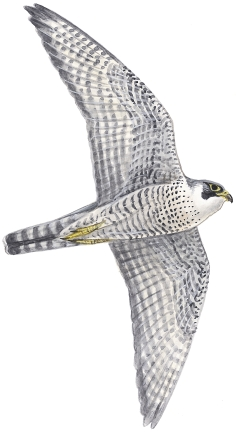
\includegraphics[height=5in]{plots/peregrine}
\vspace{4mm}

\ifthenelse{\equal{\gmxlite}{1}}
{
\fcolorbox{blue}{blue}{\textcolor{white}{\fontsize{56}{64} \selectfont User Manual {\em ~Lite~}}}
}
{
\fcolorbox{blue}{blue}{\textcolor{white}{\fontsize{56}{64} \selectfont ~USER MANUAL~}}
} % Brace matches ifthenelse test for gmxlite
\vspace{4mm}

\textcolor{blue}{\fontsize{48}{56} \selectfont ~Version \gmxver~}


%\vspace{0.25cm}
%{\fontsize{30}{36} \selectfont \bf Version \gmxver}

\end{center}
\vfill

\ifthenelse{\equal{\gmxlite}{1}} 
{
\newpage
{\bf
This text is a shortened version of the full {\gromacs} manual, written
by David van der Spoel, Berk Hess, Erik Lindahl and others. Please
find further information on our website {\wwwpage}.}

\vspace{2cm}

\noindent \copyright\ 1991--2000: 
Department of Biophysical Chemistry, University of Groningen. 
Nijenborgh 4, 9747 AG Groningen, The Netherlands.\\
\medskip

\noindent \copyright\ 2001--{\gmxyear}:
The {\gromacs} development teams at the Royal Institute of Technology and \\
Uppsala University, Sweden.
} 
{ 
\cleardoublepage
} % Brace matches ifthenelse test for gmxlite
%reset to normal margins
\addtolength{\oddsidemargin}{5mm}

%
%       P R E F A C E
%
\renewcommand{\chaptermark}[1]{\markboth{#1}{#1}} % remember chapter title
\renewcommand{\sectionmark}[1]{\markright{\thesection\ #1}}
                                                % section number and title
\lhead[\fancyplain{}{\em\thepage}]{\fancyplain{}{\em\rightmark}}
\rhead[\fancyplain{}{\em\leftmark}]{\fancyplain{}{\em\thepage}}
\cfoot{}

\ifthenelse{\equal{\gmxlite}{1}}{}{
\begin{center}
\phantom{ }
\vspace{1cm}
{\fontsize{40}{50} \selectfont 
GROMACS\\
USER MANUAL\\[1cm]
}
{\LARGE\bf Version \gmxver}\\[1cm]

{\Large 
Contributions from \\
\vspace{5mm}

Mark Abraham, Emile Apol, Rossen Apostolov, \\
Herman J.C. Berendsen, Aldert van Buuren, P\"ar Bjelkmar, \\
Rudi van Drunen, Anton Feenstra, Sebastian Fritsch, \\
Gerrit Groenhof, Christoph Junghans, Jochen Hub, Peter Kasson, \\
Carsten Kutzner, Brad Lambeth, Per Larsson, Justin A. Lemkul, \\
Erik Marklund, Peiter Meulenhoff, Teemu Murtola, \\
Szil\'ard P\'all, Sander Pronk, Roland Schulz, \\
Michael Shirts, Alfons Sijbers, Peter Tieleman and Maarten Wolf. \\}
\vspace{5mm}

{\LARGE Berk Hess, David van der Spoel, and Erik Lindahl.}
\vspace{10mm}
\end{center}

\vfill


\noindent \copyright\ 1991--2000: 
Department of Biophysical Chemistry, University of Groningen. \\
Nijenborgh 4, 9747 AG Groningen, The Netherlands.\\
\medskip

\noindent \copyright\ 2001--{\gmxyear}:
The {\gromacs} development teams at the Royal Institute of Technology and \\
Uppsala University, Sweden.

\vspace{5mm}

More information can be found on our website: {\wwwpage}.


\newpage
\pagestyle{fancyplain}

\subsection*{Preface \& Disclaimer}
This manual is not complete and has no pretention to be so due
to lack of time of the contributors -- our first priority is to improve
the software. It is worked on continuously,
which in some cases might mean the information is not entirely correct.

Comments are welcome, please send them by e-mail to {\email}, or to
one of the mailing lists (see \wwwpage).

We try to release an updated version of the manual whenever
we release a new version of the software, so in general 
it is a good idea to use a manual with the same major and
minor release number as your {\gromacs} installation. 
Any revision numbers (like 3.1.1) are however independent, 
to make it possible to implement bug fixes and manual
improvements if necessary. 

\subsection*{On-line Resources}
You can find more documentation and other material at our homepage
\wwwpage. Among other things there is an on-line reference, several
{\gromacs} mailing lists with archives and contributed
topologies/force fields.

\subsection*{Citation information}
When \normindex{citing} this document in any scientific publication
please refer to it as:
\begin{quote}
\raggedright
D. van der Spoel, E. Lindahl, B. Hess, and the GROMACS development team,
\hspace{0.3em} {\em {\gromacs} {U}ser {M}anual version \gmxver},
\hspace{0.3em} {\wwwpage} ({\gmxyear})
\end{quote}
However, we prefer that you cite (some of) the {\gromacs}
papers~\cite{Bekker93a,Berendsen95a,Lindahl2001a,Spoel2005a,Hess2008b} when you publish
your results. Any future development depends on academic research
grants, since the package is distributed as free software!

\subsection*{Current development}
{\gromacs} is a joint effort, with contributions from lots of developers around
the world. The core development is currently taking place at
\begin{itemize}
\item Department of Cellular and Molecular Biology, Uppsala University, Sweden.\\ 
(David van der Spoel).
\item Stockholm Bioinformatics Center, Stockholm University, Sweden \\
(Erik Lindahl).
\item Stockholm Bioinformatics Center, Stockholm University, Sweden \\
(Berk Hess)
\end{itemize}

\subsection*{{\gromacs} is {\em Free Software}}
The entire {\gromacs} package is available under the GNU Lesser
General Public License, version 2.1. This means it's free as in free
speech, not just that you can use it without paying us money. For
details, check the COPYING file in the source code or consult
\href{http://www.gnu.org/licenses/old-licenses/lgpl-2.1.html}{http://www.gnu.org/licenses/old-licenses/lgpl-2.1.html}.

The {\gromacs} source code and and selected set of binary packages are
available on our homepage, \wwwpage. Have fun.
} % Brace matches ifthenelse test for gmxlite

\newpage
%       C O N T E N T S
%
\tableofcontents
%\listoffigures
%\listoftables

%
%       R E A L   M A N U A L
%
\cleardoublepage
\pagenumbering{arabic}

%
% $Id$
% 
%       This source code is part of
% 
%        G   R   O   M   A   C   S
% 
% GROningen MAchine for Chemical Simulations
% 
%               VERSION 2.0
% 
% Copyright (c) 1991-1999
% BIOSON Research Institute, Dept. of Biophysical Chemistry
% University of Groningen, The Netherlands
% 
% Please refer to:
% GROMACS: A message-passing parallel molecular dynamics implementation
% H.J.C. Berendsen, D. van der Spoel and R. van Drunen
% Comp. Phys. Comm. 91, 43-56 (1995)
% 
% Also check out our WWW page:
% http://md.chem.rug.nl/~gmx
% or e-mail to:
% gromacs@chem.rug.nl
% 
% And Hey:
% Gnomes, ROck Monsters And Chili Sauce
%

\chapter{Introduction}

\section{Computational Chemistry and Molecular Modeling}

\label{sec:Compchem}

{\gromacs} is an engine to perform molecular dynamics simulations and 
energy minimization. These are two of the many techniques that belong 
to the realm of \swapindex{computational}{chemistry} and 
\swapindex{molecular}{modeling}. 
{\em Computational Chemistry} is just a name to indicate the use of 
computational techniques in chemistry, ranging from quantum mechanics 
of molecules to dynamics of large complex molecular aggregates. {\em 
Molecular modeling} indicates the general process of describing 
complex chemical systems in terms of a realistic atomic model, with the 
aim to understand and predict macroscopic properties based on detailed 
knowledge on an atomic scale. Often molecular modeling is used to 
design new materials, for which the accurate prediction of physical 
properties of realistic systems is required. 

Macroscopic physical properties can be distinguished in ($a$) {\em static 
equilibrium properties}, such as the binding constant  of an inhibitor to an 
enzyme, the average potential energy of a system, or the radial distribution  
function in a liquid, and ($b$) {\em
dynamic or non-equilibrium properties}, such as the viscosity of a 
liquid, diffusion processes in membranes, the dynamics of phase 
changes, reaction kinetics, or the dynamics of defects in crystals.  
The choice of technique depends on the question asked and on the 
feasibility of the method to yield reliable results at the present 
state of the art. Ideally, the (relativistic) time-dependent 
\swapindex{Schr{\"o}dinger}{equation} 
describes the properties of molecular systems 
with high accuracy, but anything more complex than the equilibrium 
state of a few atoms cannot be handled at this {\em ab initio} level. 
Thus approximations are necessary; the higher the complexity of a 
system and the longer the time span of the processes of interest is, 
the more severe the required approximations are. At a certain point 
(reached very much earlier than one would wish) the {\em ab initio} 
approach must be augmented or replaced by {\em empirical} 
parameterization of the model used. Where simulations based on physical 
principles of atomic interactions still fail  due to the complexity of the 
system 
molecular modeling is based entirely on a similarity analysis of known 
structural and chemical data. The \normindex{QSAR} methods (Quantitative 
Structure-Activity Relations) and many homology-based protein structure  
predictions belong to the latter category.

Macroscopic properties are always \swapindex{ensemble}{average}s over a 
representative statistical ensemble (either equilibrium or 
non-equilibrium) of molecular systems. For molecular modeling this has 
two important consequences:
\begin{itemize}
\item   The knowledge of a single structure, even if it is the structure 
        of the global energy minimum, is not sufficient. It is necessary to 
        generate a representative ensemble at a given temperature, in order to 
        compute macroscopic properties. But this is not enough to compute 
        thermodynamic equilibrium properties that are based on free energies, 
        such as phase equilibria, binding constants, solubilities,  relative 
        stability of molecular conformations, etc. The computation of free 
        energies and thermodynamic potentials requires special extensions of 
        molecular simulation techniques.
\item   While molecular simulations in principle provide atomic details 
        of the structures and motions, such details are often not relevant for 
        the macroscopic properties of interest. This opens the way to simplify 
        the description of interactions and average over irrelevant details. 
        The science of \swapindex{statistical}{mechanics} 
        provides the theoretical framework 
        for such simplifications. There is a hierarchy of methods ranging from 
        considering groups of atoms as one unit, describing motion in a 
        reduced 
        number of collective coordinates, averaging over solvent molecules 
        with 
        potentials of mean force combined with 
        \swapindex{stochastic}{dynamics}~\cite{Gunsteren90}, to {\em 
        \swapindex{mesoscopic}{dynamics}} 
        describing densities rather than atoms and fluxes 
        as response to thermodynamic gradients rather than velocities or 
        accelerations as response to forces~\cite{Fraaije93}.
\end{itemize}

For the generation of a representative equilibrium ensemble two methods 
are available: ($a$) {\em Monte Carlo simulations} and ($b$) {\em Molecular 
Dynamics simulations}. For the generation of non-equilibrium ensembles 
and for the analysis of dynamic events, only the second method is 
appropriate. While Monte Carlo simulations are more simple than MD (they 
do not require the computation of forces), they do not yield 
significantly better statistics than MD in a given amount of computer time. 
Therefore MD is the more universal technique. If a starting 
configuration is very far from equilibrium, the forces may be 
excessively large and the MD simulation may fail. In those cases a 
robust {\em energy minimization} is required. Another reason to perform 
an energy minimization is the removal of all kinetic energy from the 
system: if several 'snapshots' from dynamic simulations must be compared, 
energy minimization reduces the thermal noise in the structures and  
potential energies,  so that they can be compared better.

\section{Molecular Dynamics Simulations}
\label{sec:MDsimulations}
MD simulations solve Newton's \swapindex{equations of}{motion} 
for a system of $N$ interacting atoms:
\beq
  m_i \frac{\partial^2 \ve{r}_i}{\partial t^2}  = \ve{F}_i, \;i=1 \ldots N.
\eeq
The forces are the negative derivatives of a potential function $V(\ve{r}_1, 
\ve{r}_2, \ldots, \ve{r}_N)$:
\beq
  \ve{F}_i = - \frac{\partial V}{\partial \ve{r}_i}
\eeq
The equations are solved simultaneously in small time steps. The
system is followed for some time, taking care that the temperature and
pressure remain at the required values, and the coordinates are
written to an output file at regular intervals. The coordinates as a
function of time represent a {\em trajectory} of the system. After
initial changes, the system will usually reach an {\em equilibrium
state}. By averaging over an equilibrium trajectory many macroscopic
properties can be extracted from the output file.

It is useful at this point to consider the \normindex{limitations} of MD
simulations. The user should be aware of those limitations and always
perform checks on known experimental properties to assess the accuracy
of the simulation. We list the approximations below.

\begin{description}
\item[{\bf The simulations are classical}]\mbox{}\\
Using Newton's equation of motion automatically implies the use of
{\em classical mechanics} to describe the motion of atoms. This is
all right for most atoms at normal temperatures, but there are
exceptions. Hydrogen atoms are quite light and the motion of protons
is sometimes of essential quantum mechanical character. For example, a
proton may {\em tunnel} through a potential barrier in the course of a
transfer over a hydrogen bond. Such processes cannot be properly
treated by classical dynamics! Helium liquid at low temperature is
another example where classical mechanics breaks down. While helium
may not deeply concern us, the high frequency vibrations of covalent
bonds should make us worry! The statistical mechanics of a classical
harmonic oscillator differs appreciably from that of a real quantum
oscillator, when the resonance frequency $\nu$ approximates or exceeds
$k_BT/h$. Now at room temperature the wavenumber $\sigma = 1/\lambda =
\nu/c$ at which $h
\nu = k_BT$ is approximately 200 cm$^{-1}$. Thus all frequencies
higher than, say, 100 cm$^{-1}$ may misbehave in
classical simulations. This means that practically all bond and
bond-angle vibrations are suspect, and even hydrogen-bonded motions as
translational or librational H-bond vibrations are beyond the
classical limit (see \tabref{vibrations}). What can we do?

\begin{table}
\begin{center} 
\begin{tabular}{|l|l|r@{--}rl|}
\dline
                & \mcc{1}{type of}   & \mcc{3}{wavenumber}  \\
type of bond    & \mcc{1}{vibration} & \mcc{3}{(cm$^{-1}$)} \\
\hline
C-H, O-H, N-H   & stretch       & 3000  & 3500  & \\
C=C, C=O,       & stretch       & 1700  & 2000  & \\
HOH             & bending       & \mcl{2}{1600} & \\
C-C             & stretch       & 1400  & 1600  & \\
H$_2$CX         & sciss, rock   & 1000  & 1500  & \\ 
CCC             & bending       &  800  & 1000  & \\
O-H$\cdots$O    & libration     &  400  & 700   & \\
O-H$\cdots$O    & stretch       &   50  & 200   & \\
\dline
\end{tabular} 
\end{center} 
\caption[Typical vibrational frequencies.]{Typical vibrational
frequencies (wavenumbers) in molecules and hydrogen-bonded
liquids. Compare $kT/h = 200$ cm$^{-1}$ at 300~K.}
\label{tab:vibrations}
\end{table}

Well, apart from real quantum-dynamical simulations, we can do one
of two things: \\ (a) If we perform MD simulations using harmonic
oscillators for bonds, we should make corrections to the total
internal energy $U = E_{kin} + E_{pot}$ and specific heat $C_V$ (and
to entropy $S$ and free energy $A$ or $G$ if those are
calculated). The corrections to the energy and specific heat of a
one-dimensional oscillator with frequency $\nu$
are:~\cite{McQuarrie76}
\beq
 U^{QM} = U^{cl} +kT \left( \half x - 1 + \frac{x}{e^x-1} \right)
\eeq
\beq
 C_V^{QM} = C_V^{cl} + k \left( \frac{x^2e^x}{(e^x-1)^2} - 1 \right), 
\eeq
where $x=h\nu /kT$. The classical oscillator absorbs too much energy
($kT$), while the high-frequency quantum oscillator is in its ground
state at the zero-point energy level of $\frac{1}{2} h\nu$. \\ (b) We
can treat the bonds (and bond angles) as {\em \normindex{constraint}s}
in the equation of motion. The rational behind this is that a quantum
oscillator in its ground state resembles a constrained bond more
closely than a classical oscillator. A good practical reason for this
choice is that the algorithm can use larger time steps when the
highest frequencies are removed. In practice the time step can be made
four times as large when bonds are constrained than when they are
oscillators~\cite{Gunsteren77}. {\gromacs} has this option for the
bonds and bond angles.  The flexibility of the latter is
rather essential to allow for the realistic motion and coverage of
configurational space~\cite{Gunsteren77}.

\item[{\bf Electrons are in the ground state}]\mbox{}\\
In MD we use a {\em conservative} force field that is a
function of the positions of atoms only.  This means that the
electronic motions are not considered: the electrons are supposed to
adjust their dynamics instantly when the atomic positions change
(the {\em \normindex{Born-Oppenheimer}} approximation), and remain in
their ground state. This is really all right, almost always. But of
course, electron transfer processes and electronically excited states
can not be treated. Neither can chemical reactions be treated
properly, but there are other reasons to shy away from reactions for
the time being.

\item[{\bf Force fields are approximate}]\mbox{}\\
Force fields \index{force-field} provide the forces.
They are not really a part of the
simulation method and their parameters can be user-modified as the
need arises or knowledge improves. But the form of the forces that can
be used in a particular program is subject to limitations. The force
field that is incorporated in {\gromacs} is described in Chapter 4. In
the present version the force field is pair-additive (apart from
long-range coulomb forces), it cannot incorporate
polarizabilities, and it does not contain fine-tuning of bonded
interactions. This urges the inclusion of some limitations in this
list below.  For the rest it is quite useful and fairly reliable for
bio macro-molecules in aqueous solution!

\item[{\bf The force field is pair-additive}]\mbox{}\\
This means that all {\em non-bonded} forces result from the sum of
non-bonded pair interactions. Non pair-additive interactions, the most
important example of which is interaction through atomic
polarizability, are represented by {\em effective pair
potentials}. Only average non pair-additive contributions are
incorporated. This also means that the pair interactions are not pure,
{\ie}, they are not valid for isolated pairs or for situations
that differ appreciably from the test systems on which the models were
parameterized. In fact, the effective pair potentials are not that bad
in practice. But the omission of polarizability also means that
electrons in atoms do not provide a dielectric constant as they
should. For example, real liquid alkanes have a dielectric constant of
slightly more than 2, which reduce the long-range electrostatic
interaction between (partial) charges. Thus the simulations will
exaggerate the long-range Coulomb terms. Luckily, the next item
compensates this effect a bit.

\item[{\bf Long-range interactions are cut off}]\mbox{}\\
In this version {\gromacs} always uses a cut-off radius for the
Lennard-Jones interactions and sometimes for the Coulomb interactions
as well.  Due to the minimum-image convention (only one image of each
particle in the periodic boundary conditions is considered for a pair
interaction), the cut-off range can not exceed half the box size. That
is still pretty big for large systems, and trouble is only expected
for systems containing charged particles. But then truly bad things can
happen, like accumulation of charges at the cut-off boundary or very
wrong energies! For such systems you should consider using one of the
implemented long-range electrostatic algorithms, such as 
particle-mesh Ewald~\cite{Darden93,Essmann95}.

\item[{\bf Boundary conditions are unnatural}]\mbox{}\\
Since system size is small (even 10,000 particles is small), a cluster
of particles will have a lot of unwanted boundary with its environment
(vacuum). This we must avoid if we wish to simulate a bulk system. So
we use periodic boundary conditions, to avoid real phase
boundaries. But liquids are not crystals, so something unnatural
remains. This item is mentioned last because it is the
least of the evils. For large systems the errors are small, but for
small systems with a lot of internal spatial correlation, the periodic
boundaries may enhance internal correlation. In that case, beware and
test the influence of system size. This is especially important when
using lattice sums for long-range electrostatics, since these are known
to sometimes introduce extra ordering.
\end{description}

\section{Energy Minimization and Search Methods}

As mentioned in \secref{Compchem}, in many cases energy minimization
is required. {\gromacs} provides a number of methods for local energy
minimization, as detailed in \secref{EM}.

The potential energy function of a (macro)molecular system is a very
complex landscape (or {\em hyper surface}) in a large number of
dimensions. It has one deepest point, the {\em global minimum} and a
very large number of {\em local minima}, where all derivatives of the
potential energy function with respect to the coordinates are zero and
all second derivatives are nonnegative. The matrix of second
derivatives, which is called the {\em Hessian matrix}, has nonnegative
eigenvalues; only the collective coordinates that correspond to
translation and rotation (for an isolated molecule) have zero
eigenvalues. In between the local minima there are {\em saddle
points}, where the Hessian matrix has only one negative
eigenvalue. These points are the mountain passes through which the
system can migrate from one local minimum to another.

Knowledge of all local minima, including the global one, and of all
saddle points would enable us to describe the relevant structures and
conformations and their free energies, as well as the dynamics of
structural transitions. Unfortunately, the dimensionality of the
configurational space and the number of local minima is so high that
it is impossible to sample the space at a sufficient number of points
to obtain a complete survey. In particular, no minimization method
exists that guarantees the determination of the global minimum in any
practical amount of time [Impractical methods exist, some much faster
than others~\cite{Geman84}].  However, given a starting configuration,
it is possible to find the {\em nearest local minimum}. Nearest in
this context does not always imply nearest in a geometrical sense
({\ie}, the least sum of square coordinate differences), but means the
minimum that can be reached by systematically moving down the steepest
local gradient. Finding this nearest local minimum is all that
{\gromacs} can do for you, sorry! If you want to find other minima and
hope to discover the global minimum in the process, the best advice is
to experiment with temperature-coupled MD: run your system at a high
temperature for a while and then quench it slowly down to the required
temperature; do this repeatedly!  If something as a melting or glass
transition temperature exists, it is wise to stay for some time
slightly below that temperature and cool down slowly according to some
clever scheme, a process called {\em simulated annealing}. Since no
physical truth is required, you can use your imagination to speed up this
process. One trick that often works is to make hydrogen atoms heavier
(mass 10 or so): although that will slow down the otherwise very rapid
motions of hydrogen atoms, it will hardly influence the slower motions
in the system while enabling you to increase the time step by a factor
of 3 or 4. You can also modify the potential energy function during
the search procedure, {\eg} by removing barriers (remove dihedral
angle functions or replace repulsive potentials by {\em soft core}
potentials~\cite{Nilges88}), but always take care to restore the
correct functions slowly. The best search method that allows rather
drastic structural changes is to allow excursions into
four-dimensional space~\cite{Schaik93}, but this requires some extra
programming beyond the standard capabilities of {\gromacs}.

Three possible energy minimization methods are:
\begin{itemize}
\item   Those that require only function evaluations. Examples are the 
        simplex method and its variants. A step is made on the basis of the 
        results of previous evaluations. If derivative information is 
        available, such methods are inferior to those that use 
        this information.
\item   Those that use derivative information. Since the partial 
        derivatives of the potential energy with respect to all 
        coordinates are known in MD programs (these are equal to minus 
        the forces) this class of methods is very suitable as modification 
        of MD programs.
\item   Those that use second derivative information as well. These methods 
        are superior in their convergence properties near the minimum: a 
        quadratic potential function is minimized in one step! The problem 
        is that for $N$ particles a $3N\times 3N$ matrix must be computed, 
        stored and inverted. Apart from the extra programming to obtain 
        second derivatives, for most systems of interest this is beyond the 
        available capacity. There are intermediate methods building up the 
        Hessian matrix on the fly, but they also suffer from excessive 
        storage requirements. So {\gromacs} will shy away from this class 
        of methods.
\end{itemize}


The {\em steepest descent} method, available in {\gromacs}, is of the
second class. It simply takes a step in the direction of the negative
gradient (hence in the direction of the force), without any
consideration of the history built up in previous steps. The step size
is adjusted such that the search is fast but the motion is always
downhill. This is a simple and sturdy, but somewhat stupid, method:
its convergence can be quite slow, especially in the vicinity of the
local minimum! The faster converging {\em conjugate gradient method}
(see {\eg} \cite{Zimmerman91}) uses gradient information from previous
steps. In general, steepest descents will bring you close to the
nearest local minimum very quickly, while conjugate gradients brings
you {\em very} close to the local minimum, but performs worse far away
from the minimum. {\gromacs} also supports the L-BFGS minimizer, which
is mostly comparable to {\em conjugate gradient method}, but in some 
cases converges faster.

%
% This file is part of the GROMACS molecular simulation package.
%
% Copyright (c) 2013,2014,2015, by the GROMACS development team, led by
% Mark Abraham, David van der Spoel, Berk Hess, and Erik Lindahl,
% and including many others, as listed in the AUTHORS file in the
% top-level source directory and at http://www.gromacs.org.
%
% GROMACS is free software; you can redistribute it and/or
% modify it under the terms of the GNU Lesser General Public License
% as published by the Free Software Foundation; either version 2.1
% of the License, or (at your option) any later version.
%
% GROMACS is distributed in the hope that it will be useful,
% but WITHOUT ANY WARRANTY; without even the implied warranty of
% MERCHANTABILITY or FITNESS FOR A PARTICULAR PURPOSE.  See the GNU
% Lesser General Public License for more details.
%
% You should have received a copy of the GNU Lesser General Public
% License along with GROMACS; if not, see
% http://www.gnu.org/licenses, or write to the Free Software Foundation,
% Inc., 51 Franklin Street, Fifth Floor, Boston, MA  02110-1301  USA.
%
% If you want to redistribute modifications to GROMACS, please
% consider that scientific software is very special. Version
% control is crucial - bugs must be traceable. We will be happy to
% consider code for inclusion in the official distribution, but
% derived work must not be called official GROMACS. Details are found
% in the README & COPYING files - if they are missing, get the
% official version at http://www.gromacs.org.
%
% To help us fund GROMACS development, we humbly ask that you cite
% the research papers on the package. Check out http://www.gromacs.org.

\chapter{Definitions and Units}
\label{ch:defunits}
\section{Notation}
The following conventions for mathematical typesetting 
are used throughout this document:

\centerline{
\begin{tabular}{l|l|c}
Item		&	Notation	& Example	\\
\hline	
Vector		&	Bold italic	& $\rvi$	\\
Vector Length	&	Italic		& $r_i$		\\
\end{tabular}
}

We define the {\em lowercase} subscripts 
$i$, $j$, $k$ and $l$ to denote particles:
$\rvi$ is the {\em position vector} of particle $i$, and using this 
notation:
\bea
\rvij	=	\rvj-\rvi	\\
\rij	=	| \rvij |
\eea
The force on particle $i$ is denoted by $\ve{F}_i$ and 
\beq
\ve{F}_{ij} = \mbox{force on $i$ exerted by $j$}
\eeq
Please note that we changed notation as of version 2.0 to $\rvij=\rvj-\rvi$ since this
is the notation commonly used. If you encounter an error, let us know.

\section{\normindex{MD units}\index{units}}
{\gromacs} uses a consistent set of units that produce values in the
vicinity of unity for most relevant molecular quantities. Let us call
them {\em MD units}. The basic units in this system are nm, ps, K,
electron charge (e) and atomic mass unit (u), see
\tabref{basicunits}. The values used in {\gromacs}  are taken from the
CODATA Internationally recommended 2010 values of 
fundamental physical constants (see \verb+http://nist.gov+).
\begin{table}
\centerline{
\begin{tabular}{|l|c|l|}
\dline
Quantity	& Symbol&  Unit						\\
\hline			
length		&  r	&  nm $= 10^{-9}$ m				\\
mass		&  m	&  u (unified atomic mass unit)	$=$ 
				$1.660\,538\,921(73) \times 10^{-27}$ kg	\\
time		&  t	&  ps $= 10^{-12}$ s				\\
charge		&  q	&  {\it e} $=$ elementary charge $=
				1.602\,176\,565(35)\times 10^{-19}$ C	\\
temperature	&  T	&  K  						\\
\dline
\end{tabular}
}
\caption[Basic units used in {\gromacs}.]{Basic units used in
{\gromacs}. Numbers in parentheses give accuracy.}
\label{tab:basicunits}
\end{table}

Consistent with these units are a set of derived units, given in
\tabref{derivedunits}.
\begin{table}
\centerline{
\begin{tabular}{|l|c|l|}
\dline
Quantity	& Symbol   & Unit				\\
\hline
energy		& $E,V$	   & kJ~mol$^{-1}$			\\
Force		& $\ve{F}$ & kJ~mol$^{-1}$~nm$^{-1}$		\\
pressure	& $p$	   & kJ~mol$^{-1}$~nm$^{-3} =
				10^{30}/N_{AV}$~Pa		\\
        	&	   & $1.660\,538\,921\times 10^6$~Pa $= 
				16.605\,389\,21$~bar         		\\
velocity	& $v$	   & nm~ps$^{-1} = 1000$ m s$^{-1}$		\\
dipole moment   & $\mu$	   & \emph{e}~nm                		\\ 
electric potential& $\Phi$ & kJ~mol$^{-1}$~\emph{e}$^{-1} = 
				0.010\,364\,269\,19(32)$ Volt   	\\
electric field	& $E$	   & kJ~mol$^{-1}$~nm$^{-1}$~\emph{e}$^{-1} =
 				1.036\,426\,919(32) \times 10^7$~V m$^{-1}$	\\
\dline
\end{tabular}
}
\caption{Derived units}
\label{tab:derivedunits}
\end{table}

The {\bf electric conversion factor} $f=\frac{1}{4 \pi
\varepsilon_o}=138.935\,457\,8(39)$ kJ~mol$^{-1}$~nm~e$^{-2}$. It relates
the mechanical quantities to the electrical quantities as in
\beq
 V = f \frac{q^2}{r} \mbox{\ \ or\ \ } F = f \frac{q^2}{r^2}
\eeq

Electric potentials $\Phi$ and electric fields $\ve{E}$ are
intermediate quantities in the calculation of energies and
forces. They do not occur inside {\gromacs}. If they are used in
evaluations, there is a choice of equations and related units. We
strongly recommend following the usual practice of including the factor
$f$ in expressions that evaluate $\Phi$ and $\ve{E}$:
\bea
\Phi(\ve{r}) = f \sum_j \frac{q_j}{|\ve{r}-\ve{r}_j|} 	\\
\ve{E}(\ve{r}) = f \sum_j q_j \frac{(\ve{r}-\ve{r}_j)}{|\ve{r}-\ve{r}_j|^3}
\eea
With these definitions, $q\Phi$ is an energy and $q\ve{E}$ is a
force. The units are those given in \tabref{derivedunits}:
about 10 mV for potential. Thus, the potential of an electronic charge
at a distance of 1 nm equals $f \approx 140$ units $\approx
1.4$~V. (exact value: $1.439\,964\,5$ V)

{\bf Note} that these units are mutually consistent; changing any of the
units is likely to produce inconsistencies and is therefore {\em
strongly discouraged\/}! In particular: if \AA \ are used instead of
nm, the unit of time changes to 0.1 ps. If kcal mol$^{-1}$ (= 4.184
kJ mol$^{-1}$) is used instead of kJ mol$^{-1}$ for energy, the unit of time becomes
0.488882 ps and the unit of temperature changes to 4.184 K. But in
both cases all electrical energies go wrong, because they will still
be computed in kJ mol$^{-1}$, expecting nm as the unit of length. Although
careful rescaling of charges may still yield consistency, it is clear
that such confusions must be rigidly avoided.
  
In terms of the MD units, the usual physical constants take on
different values (see \tabref{consts}). All quantities are per mol rather than per
molecule. There is no distinction between Boltzmann's constant $k$ and
the gas constant $R$: their value is
$0.008\,314\,462\,1$~kJ~mol$^{-1}$~K$^{-1}$.
\begin{table}
\centerline{
\begin{tabular}{|c|l|l|}
\dline
Symbol	& Name			& Value					\\
\hline
$N_{AV}$& Avogadro's number 	& $6.022\,141\,29(27)\times 10^{23}$  mol$^{-1}$	\\
$R$   	& gas constant 	& $8.314\,462\,1(75)\times 10^{-3}$~kJ~mol$^{-1}$~K$^{-1}$	\\
$k_B$  	& Boltzmann's constant  & \emph{idem}	\\
$h$	& Planck's constant	& $0.399\,031\,271(17)$~kJ~mol$^{-1}$~ps \\
$\hbar$	& Dirac's constant	& $0.063\,507\,799\,3(28)$~kJ~mol$^{-1}$~ps \\
$c$	& velocity of light	& $299\,792.458$~nm~ps$^{-1}$ \\
\dline
\end{tabular}
}
\caption{Some Physical Constants}
\label{tab:consts}
\end{table}

\section{Reduced units\index{reduced units}}
When simulating Lennard-Jones (LJ) systems, it might be advantageous to
use reduced units ({\ie}, setting
$\epsilon_{ii}=\sigma_{ii}=m_i=k_B=1$ for one type of atoms). This is
possible. When specifying the input in reduced units, the output will
also be in reduced units. The one exception is the {\em
temperature}, which is expressed in $0.008\,314\,462\,1$ reduced
units. This is a consequence of using Boltzmann's constant in the
evaluation of temperature in the code. Thus not $T$, but $k_BT$, is the
reduced temperature. A {\gromacs} temperature $T=1$ means a reduced
temperature of $0.008\ldots$ units; if a reduced temperature of 1 is
required, the {\gromacs} temperature should be $120.272\,36$.

In \tabref{reduced} quantities are given for LJ potentials:
\beq
V_{LJ} = 4\epsilon \left[ \left(\frac{\sigma}{r}\right)^{12} - \left(\frac{\sigma}{r}\right)^{6} \right]
\eeq

\begin{table}
\centerline{
\begin{tabular}{|l|c|l|}
\dline
Quantity	& Symbol	& Relation to SI			\\
\hline
Length		& r$^*$  	& r $\sigma^{-1}$			\\
Mass		& m$^*$  	& m M$^{-1}$				\\
Time		& t$^*$  	& t $\sigma^{-1}$ $\sqrt{\epsilon/M}$ \\
Temperature  	& T$^*$  	& k$_B$T $\epsilon^{-1}$ 		\\
Energy		& E$^*$  	& E $\epsilon^{-1}$           	\\
Force		& F$^*$  	& F $\sigma~\epsilon^{-1}$		\\
Pressure	& P$^*$  	& P $\sigma ^3 \epsilon^{-1}$		\\
Velocity	& v$^*$  	& v $\sqrt{M/\epsilon}$		\\
Density		& $\rho^*$  	& N $\sigma ^3~V^{-1}$		\\
\dline
\end{tabular}
}
\caption{Reduced Lennard-Jones quantities}
\label{tab:reduced}
\end{table}


\section{Mixed or Double precision}
{\gromacs} can be compiled in either mixed\index{mixed
precision|see{precision, mixed}}\index{precision, mixed} or
\pawsindex{double}{precision}. Documentation of previous {\gromacs}
versions referred to ``single precision'', but the implementation
has made selective use of double precision for many years.
Using single precision
for all variables would lead to a significant reduction in accuracy.
Although in ``mixed precision'' all state vectors, i.e. particle coordinates,
velocities and forces, are stored in single precision, critical variables
are double precision. A typical example of the latter is the virial,
which is a sum over all forces in the system, which have varying signs.
In addition, in many parts of the code we managed to avoid double precision
for arithmetic, by paying attention to summation order or reorganization
of mathematical expressions. The default configuration uses mixed precision,
but it is easy to turn on double precision by adding the option
{\tt -DGMX_DOUBLE=on} to {\tt cmake}. Double precision
will be 20 to 100\% slower than mixed precision depending on the
architecture you are running on. Double precision will use somewhat
more memory and run input, energy and full-precision trajectory files
will be almost twice as large.

The energies in mixed precision are accurate up to the last decimal,
the last one or two decimals of the forces are non-significant.
The virial is less accurate than the forces, since the virial is only one
order of magnitude larger than the size of each element in the sum over
all atoms (\secref{virial}).
In most cases this is not really a problem, since the fluctuations in the
virial can be two orders of magnitude larger than the average.
Using cut-offs for the Coulomb interactions cause large errors
in the energies, forces, and virial.
Even when using a reaction-field or lattice sum method, the errors
are larger than, or comparable to, the errors due to the partial use of
single precision.
Since MD is chaotic, trajectories with very similar starting conditions will
diverge rapidly, the divergence is faster in mixed precision than in double
precision.

For most simulations, mixed precision is accurate enough.
In some cases double precision is required to get reasonable results:
\begin{itemize}
\item normal mode analysis,
for the conjugate gradient or l-bfgs minimization and the calculation and
diagonalization of the Hessian
\item long-term energy conservation, especially for large systems
\end{itemize}


% LocalWords:  ij basicunits derivedunits kJ mol mV kcal consts LJ BT
% LocalWords:  nm ps

\chapter{Algorithms}
\label{ch:algorithms}
\section{Introduction}
In this chapter we first give describe two general concepts used in
\gromacs:  {\em periodic boundary conditions} (section~\ref{sec:pbc})
and  the {\em group concept} (section~\ref{sec:group}). The MD algorithm
is desribed in section~\ref{sec:MD}: first a global form of the
algorithm is given, which is refined in subsequent subsections. The
(simple)  EM (Energy Minimization) algorithm is described in
section~\ref{sec:EM}.
Some other algorithms for special purpose dynamics are described after this.
In the final section~\ref{sec:par} of this chapter a few principles
are  given on which parallelization of {\gromacs} is based. The
parallelization  is hardly visible for the user and is therefore not
treated in detail.

A few issues are of general interest. In all cases the {\em system}
must be defined, consisting of molecules. Molecules again consist of
particles  with defined interaction functions. The detailed
description of the {\em topology} of the molecules and of the {\em force
field} and the calculation of forces is given in
chapter~\ref{ch:ff}. In the present chapter we describe
other aspects of the algorithm, such as pair list generation, update of
velocities  and positions, coupling to external temperature and
pressure,  conservation of constraints. The {\em analysis} of the data
generated by an MD simulation is treated in chapter~\ref{ch:analysis}.


\section{Periodic boundary conditions}
\label{sec:pbc}
The classical way to minimise edge effects in a finite system is to
apply {\em periodic boundary conditions}. The atoms of the system to be simulated are put into a space-filling box, which is
surrounded by translated copies of itself (Figure~\ref{fig:pbc}). 
Thus there are no
boundaries of the system; the artefact caused by unwanted
boundaries in an isolated cluster is now replaced by the artefact of
periodic conditions. If a crystal is simulated, such boundary conditions
are desired (although motions are naturally restricted to periodic
motions with wavelengths fitting into the box). If one wishes to
simulate  non-periodic systems, as liquids or solutions, the
periodicity by  itself causes errors. The errors can be evaluated by
comparing various system sizes; they are expected to be less severe than
the errors resulting from an unnatural boundary with vacuum.
\begin {figure}
\centerline{\psfig {figure=plots/pbc.eps,width=8cm,angle=270}}
\caption {Periodic boundary conditions in two dimensions.}
\label{fig:pbc}
\end {figure}

There are several possible shapes for space-filling unit cells. Some,
as the {\em truncated octahedron}~\cite{Adams79} approach a spherical
shape better than a cubic box and are therefore more economical for
studying an (approximately spherical) macromolecule in solution, since
less solvent molecules are required to fill the box given a minimum
distance between macromolecular images. However, a periodic system
based on the truncated octahedron is equivalent to a periodic system
based on a {\em triclinic} unit cell. The latter shape is the most
general space-filling unit cell; it comprises all possible
space-filling shapes~\cite{Bekker95}. Therefore {\gromacs} will in
future versions be based on the triclinic unit and will not contain
other unit cell shapes. However, in the present version
only rectangular boxes are allowed.
  

\gromacs uses exclusively periodic boundary conditions, combined
with the {\em minimum image convention:} only one - the nearest -
image of each particle is considered for non-bonded interaction terms.
The present version of \gromacs has no provisions to extend
interactions beyond the minimum image convention, e.g. to complete
lattice sums. Thus Ewald summation, Poisson solvers, or hierarchical
long-range summation methods are not implemented. We intend to
incorporate a lattice-sum method in a later version, after the best
method has been evaluated and parallelized.
  
The box can be of arbitrary dimensions, but must be rectangular. An
isolated cluster of molecules can of course be simulated as well within these
restrictions by defining the periodic box size to be much larger than
the cluster size.

The minimum image convention implies that the cut-off radius used to
truncate non-bonded interactions must not exceed half the smallest box
size:
\beq
  R_c < \half min(a,b,c),
\eeq
otherwise more than one image would be within the cut-off distance of
the force. When a macromolecule, such as a protein, is studied in
solution,  this restriction does not suffice. In principle a single
solvent  molecule should not be able
to `see' both sides of the macromolecule. This means that an edge $a$
of the box must exceed the length of the macromolecule in the
direction of that edge {\em plus} two times the cut-off radius $R_c$.
It is common to compromise in this respect, and make the solvent layer
somewhat smaller in order to reduce the computational cost.

Each unit cell (cubic, rectangular or triclinic, the latter not being
implemented in \gromacs) is surrounded by 26
translated images. Thus a particular image can always be identified by an index
pointing to one of 27 {\em translation vectors} and constructed by
applying a translation with the indexed vector (see
subsection~\ref{subsec:forces}). 

\section{The group concept}
\label{sec:group}
In the {\gromacs} MD and analysis programs one uses {\em groups} of atoms
to perform certain actions on. The maximum number of groups is 256,
but every atom can only belong to four different groups, one of each
of the following kinds:
\begin{description}
\item[T-coupling group]
The \myindex{temperature coupling} parameters (reference temperature, time
constant, number of degrees of freedom, see
subsection~\ref{subsec:update}) can be defined for each T-coupling
group separately. For example, in a solvated macromolecule the
solvent (that  tends to produce more heating by force and integration
errors)  can be coupled with a shorter time constant to a bath than a
macromolecule, or a surface can be kept cooler than an adsorbing
molecule. Many different T-coupling groups may be defined.
\item[\myindex{Freeze group}]
Atoms that belong to a freeze group are kept stationary in the
dynamics. This is useful during equilibration, e.g. to avoid that badly
placed solvent molecules will give unreasonable kicks to  protein atoms,
although the same effect can also be obtained by putting a restraining
potential on the atoms that must be protected. The freeze option can be
used on one or two coordinates of an atom, thereby freezing the atoms
in a plane or on a line. Many freeze groups can be defined.
\item[Accelerate group]
On each atom in an '\myindex{accelerate group}' an acceleration $\ve{a}^g$ will
be imposed. This is equivalent to an external force. This feature
makes it possible to drive the system into a non-equilibrium state and
enables to perform NEMD (non-equilibrium MD) to obtain transport
properties. 
\item[\myindex{Energy monitor group}]
Mutual interactions between all energy monitor
groups are compiled during
the simulation. This is done for Lennard Jones and Coulomb terms separately.
In principle up to 256 groups could be defined, but that would lead to
256$\times$256 items! Better use this concept sparingly.  
\end{description}
The use of groups in analysis programs is described in
chapter~\ref{ch:analysis}.

\section{Molecular Dynamics}
\label{sec:MD}
A global flow scheme for MD is given in Figure~\ref{fig:global}. Each
MD or  EM run requires as input a set of initial coordinates and -
optionally - initial velocities of all particles involved. This
chapter does not describe how these are obtained; for the setup of an
actual MD run check the online manual at {\wwwpage}.
\begin{figure}
\begin{center}
\addtolength{\fboxsep}{0.5cm}
\begin{shadowenv}[12cm]
{\large \bf THE GLOBAL MD ALGORITHM}
\rule{\textwidth}{2pt} \\
{\bf 1. Input initial conditions}\\[2ex]
Potential interaction $V$ as a function of atom positions\\
Positions $\ve{r}$ of all atoms in the system\\
Velocities $\ve{v}$ of all atoms in the system \\
$\Downarrow$\\
\rule{\textwidth}{1pt}\\
{\bf repeat 2,3,4} required number of steps:\\
\rule{\textwidth}{1pt}\\
{\bf 2. Compute forces} \\[1ex]
The force on any atom  \\[1ex]
$\ve{F}_i = - \frac{\partial V}{\partial \ve{r}_i}$ \\[1ex]
is computed by calculating the force between non-bonded atom pairs: \\
$\ve{F}_i = \sum_j \ve{F}_{ij}$ \\
plus the forces due to bonded interactions (which may depend on 1, 2,
3, or 4 atoms), plus restraining and/or external forces. \\
The potential and kinetic energies and the pressure tensor are computed. \\   
$\Downarrow$\\
{\bf 3. Update configuration} \\[1ex]
The movement of the atoms is simulated by numerically solving Newton's
equations of motion \\[1ex]
$\displaystyle
\frac {\de^2\ve{r}_i}{\de t^2} = \frac{\ve{F}_i}{m_i} $ \\
or \\
$\displaystyle
\frac{\de\ve{r}_i}{\de t} = \ve{v}_i ; \;\;
\frac{\de\ve{v}_i}{\de t} = \frac{\ve{F}_i}{m_i} $ \\[1ex]
$\Downarrow$ \\
{\bf 4.} if required: {\bf Output step} \\
write positions, velocities, energies, temperature, pressure, etc. \\
\end{shadowenv}
\caption{The global MD algorithm}
\label{fig:global}
\end{center}
\end{figure}

\subsection{Initial conditions}
\subsubsection*{Topology and force field}
The system topology, including a description of the force field, must
be loaded. These items are described in Chapter~\ref{ch:ff}.
All this information is static; it is never modified during the run.

\subsubsection*{Coordinates and velocities}
Then, before a run starts, the box size and the coordinates and
velocities of  all particles are required. The box size is determined
by three vectors (nine numbers) $\ve{b}_1, \ve{b}_2, \ve{b}_3$, which
represent the three basis vectors of the periodic box. While in the
present version of \gromacs only rectangular boxes are allowed, three
numbers  suffice, but the use of three vectors already
prepares for arbitrary triclinic boxes to be implemented in a later
version. 

If the run starts at $t=t_0$, the  coordinates
at $t=t_0$ must be known. The {\em leap-frog algorithm,} used to
update the time step with $\Dt$ (see subsection~\ref{subsec:update}), requires
that the velocities must be known at $t=t_0 - \hDt$. If
velocities are not available, the program can generate initial atomic
velocities $v_i, i=1\ldots 3N$ from a \myindex{Maxwellian distribution}
(Figure~\ref{fig:maxwell}) at a
given absolute temperature $T$:
\beq 
p(v_i) = \sqrt{\frac{m_i}{2 \pi kT}}\exp(-\frac{m_i v_i^2}{2kT})
\eeq
where $k$ is Boltzmann's constant (see Chapter~\ref{ch:defunits}).
\begin{figure}
\centerline{\psfig{figure=plots/maxwell.eps,angle=270,width=8cm}}
\caption{A Maxwellian distribution, generated from random numbers.}
\label{fig:maxwell}
\end{figure}
To accomplish this, normally distributed random numbers are generated
by adding twelve random numbers $R_k$ in the range $0 \le R_k < 1$ and
subtracting 6.0 from their sum. The result is then multiplied by the
standard deviation of the velocity distribution $\sqrt{kT/m_i}$. Since
the resulting total energy will not correspond exactly  to the
required temperature $T$, a correction is made: first the
centre-of-mass motion is removed and then all velocities are scaled
such that the total energy corresponds exactly to $T$ (see
eq.~\ref{eq:E-T}). 

\subsubsection*{Centre-of-mass motion}
The \myindex{centre-of-mass velocity} (c.o.m.)is normally set to zero at every step. 
Normally there is no net external force acting on the system and the c.o.m.
velocity should remain constant. In practice, however, the update
algorithm develops a very slow change in the c.o.m. velocity, and thus
in the total kinetic energy of the system, 
specially when temperature coupling is used. If such changes are not
quenched, an appreciable c.o.m. motion develops eventually in long
runs, and the temperature will be significantly misinterpreted. The
same may happen due to overall rotational motion, but only when an
isolated cluster is simulated. In periodic systems with filled boxes,
the overall rotational motion is coupled to other degrees of freedom
and does not give any problems.

\subsection{Compute forces}
\label{subsec:forces}
As mentioned in chapter~\ref{ch:ff}, internal forces are
either generated from fixed (static) lists, or from dynamics lists.
The latter concern non-bonded interactions between any pair of particles.

\subsubsection*{Pair lists generation}
The non-bonded pair forces need to be calculated only for those pairs
$i,j$  for which the distance $r_{ij}$ between $i$ and the 
\myindex{nearest image} 
of  $j$ is less than a given cut-off radius $r_c$. Some of the
particle pairs that fulfil this criterium are excluded, when their
interaction is already fully accounted for by bonded interactions. {\gromacs}
employs  a {\em pair list} that contains 
those  particle pairs for which non-bonded forces must be calculated.
The  pair list contains the particle numbers and an index for the image
displacement vectors that must be applied to  obtain the nearest
image, for  all particle pairs that
have a  nearest-image distance less than \verb'rshort'. The list is
updated  every \verb'nstlist' steps, where \verb'nstlist' is typically
10 or  20. There is an option to calculate the total non-bonded force
on each  particle due to all particle in a shell around the
list-cutoff, {\em  i.e}, at a distance between \verb'rshort' and
\verb'rlong'.  This force is calculated during the pair list update
and  retained during \verb'nstlist' steps.

The vector $\rvij = \ve{r}_j - \ve{r}_i$ connecting nearest
images is  found by constructing
\bea
x_{ij} & = & x_{ij} - a*\verb'round'(x_{ij}/a) \\
y_{ij} & = & y_{ij} - b*\verb'round'(y_{ij}/b) \\
z_{ij} & = & z_{ij} - c*\verb'round'(z_{ij}/c)
\eea
where the length of the box edges are denoted by $a,b,c$, and the
function \verb'round'($x$)  delivers the integer number that is nearest
to $x$. The translation vector index is determined by the 27
combinations of the -1, 0, or +1 values of the three \verb'round'
function results (assuming that all primary particles are in the central box).

The particles will move during the simulation, and may move outside
the primary box. Before a new pair list is made up, all particles will
be reset to the primary box, which lies in the positive quadrant with
respect to an origin at $\ve{r}_0$, by applying
\bea
x_i & = & x_i - a*\verb'round'([x_i-x_0-a/2]/a) \\
y_i & = & y_i - b*\verb'round'([y_i-y_0-b/2]/b) \\
z_i & = & z_i - c*\verb'round'([z_i-z_0-c/2]/c)
\eea

\subsubsection{Charge groups}
Where applicable, \myindex{neighbour searching} is carried out on the basis of
{\em  charge groups}. A \myindex{charge group} is a small set of nearby atoms
that  have net charge zero. Charge groups are defined in the molecular
topology. If the nearest image  distance between the {\em geometrical
centers} of the atoms of two charge groups is less than the cutoff
radius,  all atom pairs between the charge groups are included in the
pair list. This procedure avoids the creation of charges due to
the use  of a cut-off (when one charge of a dipole is within range and
the  other not), which can have disastrous consequences for the
behaviour of  the Coulomb interaction function at distances near the
cut-off  radius. If molecular groups have full charges (ions), charge
groups  do not avoid adverse cut-off effects, and the inclusing of
lattice  sums for long-range interactions must be considered (not
supplied  by {\gromacs})~\cite{Berendsen93a}. 

If appropriately
constructed \myindex{shift function}s are used for the 
\myindex{electrostatic force}s, no
charge groups are needed. Such shift functions are already implemented
in {\gromacs} (see chapter~\ref{ch:ff}) but must be used with
care: in principle they should be combined with proper computation of
long-range interactions, which is not yet implemented in \gromacs.  

The actual neighbour search is performed on a grid. The details of the
algorithm are not relevant for the user and are not given here.

\subsubsection*{Potential energy}
When forces are computed, the \myindex{potential energy} of each interaction
term is computed as well. The total potential energy is summed for
various contributions, such as Lennard Jones, Coulomb, and bonded
terms. It is also possible to compute these contributions for {\em
groups} of atoms that are separately defined (see section~\ref{sec:group}).

\subsubsection*{Kinetic energy and temperature}
The \myindex{temperature} is given by the total \myindex{kinetic energy} of the
$N$-particle system:
\beq
E_{kin} = \half \sum_{i=1}^N m_i v_i^2
\eeq
From this the absolute temperature $T$ can be computed using:
\beq
\half N_{df} kT = E_{kin}
\label{eq:E-T}
\eeq
where $k$ is Boltzmann's constant and $N_{df}$ is the number of
degrees of freedom which can be computed from:
\beq
N_{df}	~=~	3 N - N_c - 3
\eeq
Here $N_c$ is the number of {\em constraints} imposed on the system.
The additional 3 degrees of freedom must be removed because the three
centre-of-mass velocities are constants of the motion, which are usually
set to zero.  This correction is small; in the current version of
{\gromacs} it is ignored.

The kinetic energy can also be written as a tensor, which is necessary
for pressure calculation in a triclinic system, or systems where shear
forces  are imposed:
\beq
{\bf E}_{kin} = \half \sum_i^N m_i \vvi \otimes \vvi
\eeq

\subsubsection*{Pressure and virial}
The \myindex{pressure} 
tensor {\bf P} is calculated from the difference between 
kinetic energy $E_{kin}$ and the \myindex{virial} ${\bf \Xi}$
\beq
{\bf P} = \frac{2}{3 V} ({\bf E}_{kin}-{\bf \Xi})
\label{eq:P}
\eeq
where $V$ is the volume of the computational box. 
The scalar pressure $P$, which can be used for pressure coupling in the case
of isotropic systems, is computed as:
\beq
P	= {\rm trace}({\bf P})/3
\eeq

The virial ${\bf \Xi}$ tensor is defined as 
\beq
{\bf \Xi} = -\half \sum_{i<j} \rvij \otimes \Fvij 
\eeq

In Appendix~\ref{sec:virial} the
implementation  in {\gromacs} of the virial computation is described.

\subsection{Update configuration}
\label{subsec:update}

The {\gromacs} MD program utilises the so-called {\em leap-frog} 
algorithm~\cite{Hockney74} for the integration of the equations of
motion.  The \myindex{leap-frog} 
algorithm uses positions $\ve{r}$ at time $t$ and
velocities $\ve{v}$ at time $t-\hDt$; it updates positions and
velocities using the forces
$\ve{F}(t)$ determined by the positions at time $t$: 
\bea
\ve{v}(t+\hDt)	&~=~&	\ve{v}(t-\hDt)+\frac{\ve{F}(t)}{m}\Dt	\\
\ve{r}(t+\Dt)	&~=~&	\ve{r}(t)+\ve{v}(t+\hDt)\Dt
\eea
The algorithm is visualised in Figure~\ref{fig:leapfrog}.
It is equivalent to the Verlet~\cite{Verlet67} algorithm:
\beq
\ve{r}(t+\Dt)~=~2\ve{r}(t) - \ve{r}(t-\Dt) + \frac{\ve{F}(t)}{m}\Dt^2+O(\Dt^4)
\eeq
The algorithm is of third order in $\ve{r}$ and is time-reversible.
See ref.~\cite{Berendsen86b} for the merits of this algorithm and comparison
with other time integration algorithms.
 
The \myindex{equations of motion} are modified for temperature coupling
 and pressure coupling, and extended to include the conservation of
constraints, all of which are described below.
\begin {figure}
\centerline{\psfig {figure=plots/leapfrog.eps,width=8cm}}
\caption[The Leap-Frog integration method.]{The Leap-Frog integration method. The algorithm is called
Leap-Frog  (Haasje Over), because r and v are leaping
like  frogs over each others back.}
\label{fig:leapfrog}
\end {figure}

\subsubsection{Temperature coupling}
For several reasons (drift during equilibration, drift as a result of
force truncation and integration errors, heating due to external or
frictional forces), it is necessary to control the temperature of the
system. \gromacs uses the {\em weak coupling} scheme~\cite{Berendsen84}
that mimics weak coupling with first-order kinetics to an external
heat bath with given temperature $T_0$. See ref~\cite{Berendsen91} for
a comparison of this temperature control method with the
Nos\'{e}-Hoover scheme~\cite{Nose84,Hoover85}. The effect of the algorithm is
that a deviation of the system temperature from $T_0$ is slowly
corrected according to
\beq
\frac{\de T}{\de t} = \frac{T_0-T}{\tau}
\label{eq:Tcoupling}
\eeq
which means that a temperature deviation decays exponentially with a
time constant $\tau$.
This method of coupling has the advantage that the strength of the
coupling can be varied and adapted to the user requirement: for
equilibration purposes the coupling time can be taken quite short
(e.g. 0.01 ps), but for reliable equilibrium runs it can be taken much
longer (e.g. 0.5 ps) in which case it hardly influences the
conservative dynamics.
 
The heat flow into or out of the system is effected by scaling the
velocities of each particle every step with a time-dependent factor
$\lambda$, given by
\beq 
\lambda = \left[ 1 + \frac{\Delta t}{\tau_T}
\left\{\frac{T_0}{T(t -  \hDt)} - 1 \right\} \right]^{1/2}
\label{eq:lambda}
\eeq
The parameter $\tau_T$ is close to, but not exactly equal to the time constant
$\tau$ of the \myindex{temperature coupling} (eq.~\ref{eq:Tcoupling}):
\beq
\tau = 2 C_V \tau_T / N_{df} k
\eeq
where $C_V$ is the total heat capacity of the system, $k$ is Boltzmann's
constant, and $N_{df}$ is the total number of degrees of freedom. The
reason that $\tau \neq \tau_T$ is that the kinetic energy change
caused by scaling the velocities is partly redistributed between
kinetic and potential energy and hence the change in temperature is
less than the scaling energy.  In practice, the ratio $\tau / \tau_T$
ranges from 1 (gas) to 2 (harmonic solid) to 3 (water). When we use
the term 'temperature coupling time constant', we mean the parameter
\normindex{$\tau_T$}.  
{\bf Note} that in practice the scaling factor $\lambda$ is limited to 
the range of 0.8 $<= \lambda <=$ 1.25, to avoid scaling by very large
numbers which may crash the simulation. In normal use, 
$\lambda$ will allways be much closer to 1.0.
  
Strictly,  for computing the scaling factor the temperature $T$ is
needed at time $t$, but this is not available in the algorithm. In
practice, the temperature at the previous time step is used (as
indicated in eq.~\ref{eq:lambda}), which is
perfectly allright since the coupling time constant is much longer
than one time step. The algorithm is stable up to $\tau_T \approx \Dt$.

\subsubsection*{Pressure coupling}
In the same spirit as the temperature coupling, the system can also be
coupled to a '\myindex{pressure bath}'. 
This is accomplished~\cite{Berendsen84} by scaling
coordinates and box size every step with a parameter $\mu$, which has
the effect of a first-order kinetic relaxation of the pressure towards
a given reference pressure $P_0$:
\beq
\frac{\de P}{\de t} = \frac{P_0-P}{\tau_p}
\eeq
The scaling factor is given by
\beq
\mu = \left[ 1 + \frac{\Delta t}{\tau_p} \beta \{P(t) - P_0 \}
\right]^{1/3}
\label{eq:mu}
\eeq
Here $\beta$ is the isothermal compressibility of the system. In general
this is not known. It suffices to take a rough estimate because the
value of $\beta$ only influences the non-critical time constant of the
pressure relaxation without affecting the average pressure itself. For
water at 300 K $\beta = 4.6 \times 10^{-10}$ Pa$^{-1}$, which is $7.6
\times 10^{-4}$ MD units (see chapter~\ref{ch:defunits}). Most other
liquids have similar values.

In the present version of \gromacs the pressure coupling can be done
anisotropically: the $x,y,z$ dimensions are scaled separately, based
on the diagonal elements of the pressure tensor. This allows e.g.  to couple
one dimension to an external pressure, while keeping a fixed surface
area in the other two dimensions (useful in membrane simulations). The
system  axes remain orthogonal (the scaling method allows in principle
also  dynamic changes in box angles, but this is not implemented yet).

Since the pressure fluctuates heavily, it is recommended to take
$\tau_p$ not too small; a value between 0.4 and 1 ps will often be
satisfactory.

\subsubsection*{The complete update algorithm}
The complete algorithm for the update of velocities and coordinates is
given in figure~\ref{fig:complete-update}. The SHAKE algorithm of step
4 is explained below. 
\begin{figure}
\begin{center}
\addtolength{\fboxsep}{0.5cm}
\begin{shadowenv}[12cm]
{\large \bf THE UPDATE ALGORITHM}
\rule{\textwidth}{2pt} \\
Given:\\
Positions $\ve{r}$ of all atoms at time $t$ \\
Velocities $\ve{v}$ of all atoms at time $t-\hDt$ \\
Accelerations $\ve{F}/m$ on all atoms at time $t$.\\
(Forces are computed disregarding any constraints)\\
Total kinetic energy and virial \\
$\Downarrow$ \\
{\bf 1.} Compute the scaling factors $\lambda$ and $\mu$\\
according to eqs~\ref{eq:lambda} and \ref{eq:mu}\\   
$\Downarrow$ \\
{\bf 2.} Update and scale velocities: $\ve{v}' =  \lambda (\ve{v} +
\ve{a} \Delta t)$ \\
$\Downarrow$ \\
{\bf 3.} Compute new unconstrained coordinates: $\ve{r}' = \ve{r} + \ve{v}'
\Delta t$ \\
$\Downarrow$ \\
{\bf 4.} Apply constraint algorithm to coordinates: constrain($\ve{r}^{'} \rightarrow  \ve{r}'';
\,  \ve{r}$) \\
$\Downarrow$ \\
{\bf 5.} Correct velocities for constraints: $\ve{v} = (\ve{r}'' -
\ve{r}) / \Delta t$ \\
$\Downarrow$ \\
{\bf 6.} Scale coordinates and box: $\ve{r} = \mu \ve{r}''; \ve{b} =
\mu  \ve{b}$ \\
\end{shadowenv}
\caption{The MD update algorithm}
\label{fig:complete-update}
\end{center}
\end{figure}

\gromacs has a provision to ''freeze''  (prevent motion of) selected
particles, which must be defined as a 'freeze group'. This is implemented
using a {\em freezefactor $\ve{f}_g$}, which is a vector, and differs for each
{\em freezegroup} (see section~\ref{sec:group}). This vector contains only
zero (freeze) or one (don't freeze).
When we take this freezefactor and the external acceleration $\ve{a}_h$ into 
account the update algorithm for the velocities becomes:
\beq
\ve{v}(t+\hdt)~=~\ve{f}_g * \lambda * \left[ \ve{v}(t-\hdt) +\frac{\ve{F}(t)}{m}\Delta t + \ve{a}_h \Delta t \right]
\eeq
where $g$ and $h$ are group indices which differ per atom.

\subsection{Constraint algorithms}

\subsubsection*{SHAKE}
\myindex{Constraints} can be imposed in {\gromacs} using the traditional 
\myindex{SHAKE}
method~\cite{Ryckaert77}. The SHAKE routine changes a set of unconstrained
coordinates $\ve{r}^{'}$ to a set of coordinates $\ve{r}''$ that
fulfil a  list of distance constraints, using a set $\ve{r}$ as
reference: \\[1ex] 
\hspace*{5em} SHAKE($\ve{r}^{'} \rightarrow  \ve{r}'';\,  \ve{r}$) \\[1ex]
This action is consistent with solving a set of Lagrange multipliers
in the constrained equations of motion. SHAKE needs a {\em tolerance}
\verb'TOL'; it will continue until all constraints are satisfied
within a {\em relative} tolerance \verb'TOL'. An error message is
given if SHAKE cannot reset the coordinates because the deviation is
too large, or if a given number of iterations is surpassed. 

Assume the equations of motion must fulfil $K$ holonomic constraints,
expressed as
\beq
\sigma_k(\ve{r}_1 \ldots \ve{r}_N) = 0; \;\; k=1 \ldots K
\eeq
(e.g. $(\ve{r}_1 - \ve{r}_2)^2 - b^2 = 0$). 
Then the forces are defined as 
\beq
- \frac{\partial}{\partial \ve{r}_i} \left( V + \sum_{k=1}^K \lambda_k
\sigma_k \right)
\eeq
where $\lambda_k$ are Lagrange multipliers which must be solved to
fulfil the constraint equations. The second part of this sum
determines the {\em constraint forces} $\ve{G}_i$, defined by
\beq
\ve{G}_i = -\sum_{k=1}^K \lambda_k \frac{\partial \sigma_k}{\partial
\ve{r}_i}
\eeq
The displacement due to the constraint forces in the leap frog or
Verlet algorithm is equal to $(\ve{G}_i/m_i)(\Dt)^2$. Solving the
Lagrange multipliers (and hence the displacements) requires the
solution of a set of coupled equations of the second degree. These are
solved iteratively by SHAKE.
For the special case of rigid water molecules, that often make up more
than 80\% of the simulation system we have implemented the 
\myindex{SETTLE}
algorithm~\cite{Miyamoto92} (Sec~\ref{sec:settle}).


\newcommand{\fs}{\begin{equation} \label}
\newcommand{\fe}{\end{equation}}
\newcommand{\p}{\partial}
\newcommand{\Bm}{\ve{B}}
\newcommand{\M}{\ve{M}}
\newcommand{\iM}{\M^{-1}}
\newcommand{\Tm}{\ve{T}}
\newcommand{\Sm}{\ve{S}}
\newcommand{\fo}{\ve{f}}
\newcommand{\con}{\ve{g}}
\newcommand{\lenc}{\ve{d}}

\subsubsection*{The LINCS algorithm}
\myindex{LINCS} is an algorithm that resets bonds to their correct lengths
after an unconstrained update~\cite{Hess97}. 
The method is non-iterative, as it always uses two steps.
Altough LINCS is based on matrices, no matrix-matrix multiplications are 
needed. The method is more stable and faster than SHAKE, 
but it can only be used with bond \myindex{constraints} and 
isolated angle constraints, such as the proton angle in OH. 
Because of its stability LINCS is especially useful for Langevin Dynamics. 
LINCS has two parameters, which are explained in the subsection parameters.
 
\subsubsection*{The LINCS formulas}
We consider a system of $N$ particles, with positions given by a
$3N$ vector $\ve{r}(t)$.
For Molecular Dynamics the equations of motion are given by Newton's law
\fs{c1}
{\de^2 \ve{r} \over \de t^2} = \iM \ve{F}
\fe
where $\ve{F}$ is the $3N$ force vector 
and $\M$ is a $3N \times 3N$ diagonal matrix,
containing the masses of the particles.
The system is constrained by $K$ time-independent constraint equations
\fs{c2}
g_i(\ve{r}) = | \ve{r}_{i_1}-\ve{r}_{i_2} | - d_i = 0 ~~~~~~i=1,\ldots,K
\fe

In a numerical integration scheme LINCS is applied after an 
unconstrained update, just like SHAKE.
The algorithm works in two steps (see figure \ref{lincs_fig}).
In the first step the projections of the new bonds on the old
bonds are set to zero. In the second step a correction is 
applied for the lengthening of the bonds due to rotation.
The numerics for the first step and the second step are very similar. 
A complete derivation of the algorithm can be found in \cite{Hess97}.
Only a short description of the first step is given here.
\begin{figure}
\centerline{\psfig{figure=plots/lincs.eps,height=50mm}}
\caption{
\label{lincs_fig}Schematic picture showing the three position updates needed 
for one timestep. 
The dashed line is the old bond of length $d$, 
the solid lines are the new bonds.
$l=d \cos \theta$ 
and $p=(2 d^2 - l^2)^{1 \over 2}$.
}
\end{figure}

A new notation is introduced for the gradient matrix of the constraint 
equations which appears on the right hand side of the equation
\fs{c3}
B_{hi} = {\p g_h \over \p r_i}
\fe
Notice that $\Bm$ is a $K \times 3N$ matrix, it contains the directions
of the constraints.
The following equation shows how the new constrained coordinates 
$\ve{r}_{n+1}$ are related to the unconstrained coordinates
$\ve{r}_{n+1}^{unc}$
\fs{m0}
\begin{array}{c}
  \ve{r}_{n+1}=(\ve{I}-\Tm_n \ve{B}_n) \ve{r}_{n+1}^{unc} + \Tm_n \lenc=  
  \\[2mm]
  \ve{r}_{n+1}^{unc} - 
\iM \Bm_n (\Bm_n \iM \Bm_n^T)^{-1} (\Bm_n \ve{r}_{n+1}^{unc} - \lenc) 
\end{array}
\fe
where $\Tm = \iM \Bm^T (\Bm \iM \Bm^T)^{-1}$.
The derivation of this equation from \ref{c1} and \ref{c2} can be found
in \cite{Hess97}.

Half of the CPU time goes to inverting the constraint coupling 
matrix $\Bm_n \iM \Bm_n^T$, which has to be done every time step.
This $K \times K$ matrix
has $1/m_{i_1} + 1/m_{i_2}$ on the diagonal.
The off-diagonal elements are only non-zero when two bonds are connected,
then the element is 
$\cos \phi /m_c$,  where $m_c$ is 
the mass of the atom connecting the
two bonds and $\phi$ is the angle between the bonds.

The matrix $\Tm$ is inverted through a power expansion.
A $K \times K$ matrix $\ve{S}$ is 
introduced which is the inverse square root of 
the diagonal of $\Bm_n \iM \Bm_n^T$.
This matrix is used to convert the diagonal elements 
of the coupling matrix to one
\fs{m2}
\begin{array}{c}
(\Bm_n \iM \Bm_n^T)^{-1}
= \Sm \Sm^{-1} (\Bm_n \iM \Bm_n^T)^{-1} \Sm^{-1} \Sm  \\[2mm]
= \Sm (\Sm \Bm_n \iM \Bm_n^T \Sm)^{-1} \Sm =
  \Sm (\ve{I} - \ve{A}_n)^{-1} \Sm
\end{array}
\fe
The matrix $\ve{A}_n$ is symmetric and sparse and has zeros on the diagonal.
Thus a simple trick can be used to calculate the inverse
\fs{m3}
(\ve{I}-\ve{A}_n)^{-1}= 
	\ve{I} + \ve{A}_n + \ve{A}_n^2 + \ve{A}_n^3 + \ldots
\fe

This inversion method is only valid if the absolute values of all the
eigenvalues of $\ve{A}_n$ are smaller than one.
In molecules with only bond constraints the connectivity is so low
that this will always be true, even if ring structures are present.
Problems can arise in angle-constrained molecules.
By constraining angles with additional distance constraints
multiple small ring structures are introduced.
This gives a high connectivity, leading to large eigenvalues.
Therefore LINCS should NOT be used with coupled angle-constraints.

\subsubsection*{The LINCS Parameters}
The accuracy of LINCS depends on the number of matrices used
in the expansion \ref{m3}. For MD calculations a fourth order
expansion is enough. For Position Langevin Dynamics with
large timesteps an eighth order expansion may be neccesary.
The order is a parameter in the input file for \verb'mdrun'.
The implementation of LINCS is done in such a way that the 
algorithm will never crash. Even when it is impossible to
to reset the constraints LINCS will generate a conformation
which fulfills the constraints as well as possible.
However, LINCS will generate a warning when in one step a bond 
rotates over more than a predefined angle.
This angle is set by the user in the input file for \verb'mdrun'.


\subsection{Output step}
The important output of the MD run is the {\em
\myindex{trajectory file}} \verb'name.trj' which contains particle coordinates
and -optionally- velocities at regular intervals. Since the trajectory
files are lengthy, one should not save every step! To retain all
information it suffices to write a frame every 15 steps, since at
least 30 steps are made per period of the highest frequency in the
system, and Shannon's \myindex{sampling} theorem states that two samples per
period of the highest frequency in a band-limited signal contain all
available information. But that still gives very long files! So, if
the highest frequencies are not of interest, 10 or 20 samples per ps
may suffice. Be aware of the distortion of high-frequency motions by
the {\em stroboscopic effect}, called {\em aliasing}: higher frequencies
are  mirrored with respect to the sampling frequency and appear as
lower frequencies. 

A more detailed flow sheet of the MD algorithm is given in
fig.~\ref{fig:flowdetail}. 

\begin{figure}
\begin{center}
\addtolength{\fboxsep}{0.5cm}
\begin{shadowenv}[12cm]
{\large \bf THE MD ALGORITHM}
\rule{\textwidth}{2pt} \\
{\bf Input initial conditions} \\[2ex]
Potential interaction $V$ as a function of atom positions \\
Positions $\ve{r}$ of all atoms at time $t$ \\
(Velocities $\ve{v}$ of all atoms at time $t-\hDt$) \\
$\Downarrow$ \\
(if required:) Generate initial velocities; reset c.o.m. velocity to
zero; correct velocities for exact temperature \\
$\Downarrow$ \\
{\bf repeat} required number of blocks of $n$ steps:
\begin{shadowenv}[10cm]
reset particles into primary box \\
$\Downarrow$ \\
generate pair list and compute shell forces\\
$\Downarrow$ \\
{\bf repeat} $n$ times:
\begin{shadowenv}[8cm]
reset c.o.m. velocities \\
$\Downarrow$ \\
update configuration \\
(if required:) output step
\end{shadowenv}
\end{shadowenv}
\end{shadowenv}
\caption{the MD algorithm}
\label{fig:flowdetail}
\end{center}  
\end{figure}

\section{Simulated Annealing}
\label{sec:SA}
The well known \myindex{simulated annealing}
(SA) protocol is implemented
in a simple way into {\gromacs}. A modification of the temperature coupling
scheme is used as a very basic implementation of the SA algorithm. The
method works as follows: the reference temperature for coupling $T_0$
(eq.~\ref{eq:Tcoupling})
is not constant but can be varied linearly:
\beq
T_0({\rm step}) = T_0 * (\lambda_0 + \Delta\lambda * {\rm step})
\label{eq:SA}
\eeq
if $\lambda_0$ = 1 and $\Delta\lambda$ is 0 this is the plain MD
algorithm. Note that for standard SA $\Delta\lambda$  must be negative.
When $T_0$(step) $<$ 0 it is set to 0, as negative temperatures do not have
a physical meaning. This ``feature'' 
allows for an annealing strategy in which
at first the temperature is scaled down linearly until 0 K, 
and when more steps
are taken the simulation proceeds at 0 K. Since the weak coupling scheme
does not couple instantaneously, the actual temperature will
always be slightly higher than 0 K.

\section{Langevin Dynamics}
\newcommand{\vrond}{\stackrel{\circ}{\ve{r}}}
\newcommand{\rond}{\stackrel{\circ}{r}}
\newcommand{\ruis}{\ve{r}^G}
\label{sec:LD}
The Position Langevin Dynamics algorithm is implemented in {\gromacs} is 
(note: NOT {\em Velocity} Langevin Dynamics). 
This applies to overdamped systems, 
i.e. systems in which the inertia effects are negligible.
The equations are
\beq
{\de \ve{r} \over \de t} = {\ve{F}(\ve{r}) \over \gamma} + \vrond
\eeq 
where $\gamma$ is the friction coefficient $[\mbox{amu/ps}]$ and
$\vrond(t)$  is a noise process with 
$\langle \rond_i\!(t) \rond_j\!(0) \rangle = 
    2 \delta(t) \delta_{ij} k_b T / \gamma$.
In {\gromacs} the equations are integrated with an explicit scheme
\beq
\ve{r}_{n+1} = \ve{r}_{n} +
	{\Delta t \over \gamma} \ve{F}(\ve{r}_n) 
	+ \sqrt{2 k_b T {\Delta t \over \gamma}}\, \ruis 
\eeq
where $\ruis$ is  Gaussian distributed noise with $\mu = 0$, $\sigma = 1$.
Because the system is assumed to be overdamped, large timesteps
can be used. LINCS should be used for the constraints since SHAKE
will not converge for large atomic displacements.
LD is an option of the \verb'mdrun' program.

\section{Energy Minimisation}
\label{sec:EM}
Energy minimisation in {\gromacs} can be done using a  simple 
\myindex{steepest descent} method. 
\myindex{Conjugate gradient} minimization is planned for the
next release. EM is just an option of the \verb'mdrun' program.

\subsection{Steepest Descents.}
Although Steepest Descents is certainly not the most efficient
algorithm for searching, it is robust and easy to implement.
It can not be used with SHAKE, so explicit bond interactions must be
specified in the topology.

We define the vector $\ve{r}$ as the vector of all $3N$ coordinates.
Initially a maximum displacement $h_0$ (e.g. 0.01 nm) must be given. 

First the forces $\ve{F}$ and potential energy are calculated.
New positions are calculated by
\beq
\ve{r}_{n+1} =	\ve{r}_n + \frac{\ve{F}_n}{\max (|\ve{F}_n|)} h_n
\eeq
where $h_n$ is the maximum displacement and $\ve{F}_n$ is the force,
or the negative gradient of the  potential $V$. The notation $\max
(|\ve{F}_n|)$ means the largest of the absolute values of the force
components.  The forces and energy are again computed for the new positions \\
If ($V_{n+1} < V_n$) the new positions are accepted and $h_{n+1} = 1.2
h_n$. \\
If ($V_{n+1} \geq V_n$) the new positions are rejected and $h_n = 0.2 h_n$.

The algorithm stops when either a user specified number of force 
evaluations has been performed (e.g. 100), or when the maximum of the absolute
values of the force (gradient) components is smaller than a specified
value $\epsilon$.
Since force truncation produces some noise in the
energy evaluation, the stopping criterium should not be made too tight
to avoid endless iterations. A reasonable value for $\epsilon$ can be
estimated from the rms force $f$ a harmonic oscillator would exhibit at a
temperature $T$ This value is 
\beq
  f = 2 \pi \nu \sqrt{ 2mkT}
\eeq
where $\nu$ is the oscillator frequency, $m$ the (reduced) mass, and
$k$ Boltzmann's constant. For a weak oscillator with a wave number of
100 cm$^{-1}$ and a mass of 10 atomic units, at a temperature of 1 K,
$f=7.7$ kJ~mol$^{-1}$~nm$^{-1}$. A value for $\epsilon$ between 1 and
10 is acceptable.   

%\subsection{Conjugate Gradients}
%\NI

\section{Normal Mode Analysis}
\myindex{Normal mode analysis}~\cite{Levitt83,Go83,BBrooks83b} 
can be performed using {\gromacs}, by diagonalization of the mass-weighted
\myindex{Hessian}:
\beq
M^{-1/2} H M^{-1/2} Q	~=~	\omega^2 Q
\eeq
where $M$ contains the atomic masses, $Q$ contains eigenvectors, and $\omega$
contains the corresponding eigenvalues (frequencies).

First, the Hessian matrix, which is a 3N x 3N matrix where N is the number
of atoms, has to be calculated:
\beq
H_{ij}	~=~	\frac{\partial^2 V}{\partial x_i \partial x_j}
\eeq
where $x_i$ and $x_j$ denote the atomic x,y or z coordinates.
In practice, these equations have not been developed analytically, but
the force is used
\beq
F_i	~=~	\frac{\partial V}{\partial x_i}
\eeq
from which the Hessian is computed numerically. It should be noted that
for a usual Normal Mode calculation, it is necessary to completely minimize 
the energy prior to computation
of the Hessian. A number of {\gromacs} programs are involved in these
calculations. First \myindex{nmrun}, which computes the Hessian,
and secondly \myindex{g\_nmeig} which does the diagonalization and
sorting of normal modes according to frequencies. Both these programs
should be run in double precision. An overview of normal mode analysis
and the related \myindex{essential dynamics} or
\myindex{principal component analysis} can be found in ~\cite{Hayward95b}.

\section{Free energy perturbation}
\label{sec:fepalg}
\normindex{Free energy perturbation} calculations can be performed
in {\gromacs} using slow-growth methods. An example problem might be:
calculate the difference in free energy of binding of an inhibitor {\bf I}
to an enzyme {\bf E} and to a mutated enzyme {\bf E'}.
It is not feasible with computer simulations to perform a docking
calculation for such a large complex, or even releasing the inhibitor from
the enzyme in a reasonable amount of computer time with reasonable accuracy.
However, if we consider the free energy cycle in (\figref{free}A)
we can write
\beq
\Delta G_1 - \Delta G_2	=	\Delta G_3 - \Delta G_4
\label{eqn:ddg}
\eeq
If we are interested in the left-hand term we can equally well compute
the right-hand term.
\begin{figure}
\centerline{\psfig{figure=plots/free1.eps,width=6cm,angle=270}\hspace{2cm}\psfig{figure=plots/free2.eps,width=6cm,angle=270}}
\caption{Free energy cycles. {\bf A:} to calculate $\Delta G_{12}$ or the free energy difference between the binding of inhibitor {\bf I} to enzymes {\bf E} respectively {\bf E'}. {\bf B:} to calculate $\Delta G_{12}$ which is the free energy difference for binding of inhibitors {\bf I} respectively {\bf I'} to enzyme {\bf E}.}
\label{fig:free}
\end{figure}

If we want to compute the difference in free energy of binding of two
inhibitors {\bf I} and {\bf I'} to an enzyme {\bf E} (\figref{free}B)
we can again use \eqnref{ddg} to compute the desired property.

\section{Essential Dynamics Sampling}
The results from an Essential Dynamics (ED) analysis \cite{Amadei93}
of a protein can be used to guide MD simulations. The idea is that
from an initial MD simulation (or from other sources) a definition of
the collective fluctuations with largest amplitude is obtained. The
position along one or more of these collective modes can be
constrained in a (second) MD simulation in a number of ways for
several purposes. For example, the position along a certain mode may
be kept fixed to monitor the average force (free-energy gradient) on
that coordinate in that posistion. Another application is to enhance
sampling efficiency with respect to usual MD
\cite{Degroot96a,Degroot96b}. In this case, the system is encouraged
to sample its available configuration space more systematically than
in a diffusion-like path that proteins usually take.

All available constraint types are described in the appropriate chapter
of the WHAT IF \cite{Whatif} manual.


\section{Parallelization}
\label{sec:par}

\newcommand{\abs}[1]{\mid \! {#1} \! \mid}

The purpose of this section is to discuss the 
\myindex{parallelisation} of the 
principle MD algorithm and not to describe the algorithms that are in 
practical use for molecular systems with their complex variety of atoms 
and terms in the force field descriptions. We shall therefore consider 
as an example a simple system consisting only of a single type of atoms 
with a simple form of the interaction potential. The emphasis will be 
on the special problems that arise when the algorithm is implemented on 
a parallel computer. 

The simple model problem already contains the bottleneck of all MD 
simulations: the computationally intensive evaluation of the 
{\em nonbonded} forces between pairs of atoms, based on the distance 
between particles. Complex molecular systems will in addition 
involve many different kinds of {\em bonded} forces between designated 
atoms. Such interactions add to the complexity of the algorithm but do 
not modify the basic considerations concerning parallelization.


\subsection{Methods of parallelisation}
There are a number of methods to parallelise the MD algorithm, each of
them with their own advantages and disadvantages. The method to 
choose depends on the hardware and compilers available.
We list them here:
\begin{enumerate}
\item[1]	{\em \myindex{Message Passing}.}\\
		In this method, which is more or less the traditional
		way of parallel programming, all the parallelism is
		explicitly programmed by the user. The disadvantage
		is that it takes extra code and effort, the advantage
		is that the programmer keeps full control over the data
		flow and can do optimisations a compiler could not come 
		up with. 

		The implementation is typically done by calling a set of 
		library routines to send and receive data to and from 
		other processors. Almost all hardware vendors support 
		this way of
		parallellism in their C and Fortran compilers.
		
\item[2]	{\em \myindex{Data Parallel}.}\\
		This method lets the user define arrays on which to
		operate in parallel. Programming this way is much
		like vectorising: recurrence is not parallelised
		(eg. {\tt for(i=1; (i<MAX); i++) a[i] = a[i-1] + 1;}
		does not vectorise and not parallelise, because for
		every i the result from the previous step is needed).

		The advantage of data parallellism is that it is
		easier for the user; the compiler takes care of the
		parallellism. The disadvantage is that it is supported
		by a small (though growing) number of hardware vendors,
		and that it is much harder to maintain a program that has to
		run on both parallel and sequential machines, because
		the only standard language that supports it is Fortran-90
		which is not available on many platforms.
\end{enumerate}
Both methods allow for the MD algorithm to be implemented without much
trouble. Message passing MD algorithms have been published
since the mid 80's (\cite{Fincham87}, \cite{Raine89}) 
and development is still continuing. 
Data parallel programming is newer,
but starting from a well vectorised program it is not hard to do.

Our implementation of MD is a message passing one, the reason for which
is partly historical: the project to develop a parallel MD progam started
when Fortran-90 was still in the making, and no compilers were
expected to be available. 
At current, we still believe that message passing is the way
to go, after having done some experiments with data parallel programming on a
Connection Machine (CM-5), because of portability to other hardware,
the poor performance of the code produced by the compilers 
and because this way of programming
has the same drawback as vectorisation: the part of the program that is
not vectorised or parallellised determines the runtime of the program
(\myindex{Amdahl's law}).

The approach we took to parallellism was a minimalist one: use as little
non-standard elements in the software as possible, and use the
simplest \myindex{processor topology} that does the job. We therefore 
decided to use a standard language (Ansi-C) with as little non-standard
routines as possible. We only use 5 communication routines that are
non-standard. It is therefore very easy to port our code to other machines.

For an $O(N^2)$ problem like MD, one of the best schemes for the 
interprocessor connections is a ring, so our software demands that
a ring is present in the interprocessor connections. A ring can 
almost always be mapped onto another network like a \myindex{hypercube}, a bus
interface (ethernet eg. using Parallel Virtual Machines PVM~\cite{pvm3})
or a \myindex{tree} (CM-5). Some hardware vendors
have very luxurious connection schemes that connect every processor
to every other processor, but we do not really need it and so do not use
it even though it might come in handy at times.

When using a message passing scheme one has to divide the particles 
over processors, which can be done in two ways:
\begin{itemize}
\item	{\em \myindex{Space Decomposition}.}\\
	An element of space is allocated to each processor, when dividing
	a cubic box with edge $b$ over $P$ processors this can be done 
	by giving
	each processor a slab of length $b/P$. This method 
	has the advantage
	that each processor has about the same number of interactions
	to calculate (at least when the simulated system has a homogeneous
	density, like a liquid or a gas). The disadvantage is that a lot of
	bookkeeping is necessary for particles that move over processor
	boundaries. When using more complex systems like macromolecules there
	are also 3- and 4-atom interactions that would 
	complicate the bookkeeping so much that this method is not used
	in our program.
\item	{\em \myindex{Particle Decomposition}.}\\
	Every processor is allocated a number of particles. When
	dividing $N$ particles over $P$ processors each processor will
	get $N/P$ particles. The implementation of this method
	is described in the next section.
\end{itemize}

\subsection{MD on a ring of processors}
When a neighbourlist is not used the MD problem is in principle an $O(N^2)$ 
problem as each particle can interact
with every other. This can be simplified using Newtons third law
\beq
F_{ij}	~=~	-F_{ji}
\label{Eq:Newt3}
\eeq
This implies that there is half a matrix of interactions (without diagonal, 
a particle does not interact with itself) to consider 
(Figure~\ref{Fig:int_mat}).
\begin {figure}
\centerline{\psfig{figure=plots/int_mat.eps,width=10cm}}
\caption {The interaction matrix (left) and the same using action=-reaction (right).}
\label{Fig:int_mat}
\end {figure}
When we reflect the upper right triangle of interactions to the lower left
triangle of the matrix, we still cover all possible interactions, but now
every row in the matrix has almost
the same number of points or possible interactions.
We can now assign a (preferrably equal) number of rows to each processor
to compute the forces and at the same time a number of particles to
do the update on, the {\em home} particles. The number of interactions
per particle is dependent on the {\em total number} $N$ of particles
(see Figure~\ref{Fig:decomp}) and on the {\em particle number} $i$.
The exact formulae are given in Table~\ref{Tab:decomp}
\begin{table}
\caption{The number of $j$ particles per $i$ particle is a function of the total number of particles $N$ and particle number $i$. Note that the / operator implies integer division, ie. with truncation.}
\captspace
\label{Tab:decomp}
\centerline{
\begin{tabular}{l|c|c|c|c}
\dline
	   & i mod 2 = 0 & i mod 2 = 0 	& i mod 2 = 1	& i mod 2 = 1 \T \\
	   & i $<$ N/2& i $\ge$ N/2 	& i $<$ N/2	& i $\ge$ N/2 \B \\
\hline
N mod 2 = 1 & N/2	& N/2		& N/2		& N/2	\T	\\
N mod 4 = 2 & N/2	& N/2 		& N/2 - 1	& N/2 - 1	\\
N mod 4 = 0 & N/2	& N/2 - 1	& N/2 - 1	& N/2 	\B	\\
\dline
\end{tabular}
}
\end{table}

\begin {figure}
\centerline{\psfig {figure=plots/decomp.eps,width=\linewidth}}
\caption[Interaction matrices for different $N$.]{Interaction matrices for different $N$. The number of $j$-particles an $i$-particle interacts with depends on the {\em total} number of particles and on the {\em particle number}.}
\label{Fig:decomp}
\end {figure}

A flow chart of the algorithm is given in Figure~\ref{Fig:mdpar}.
\begin {figure}
\centerline{\psfig {figure=plots/mdpar.eps,width=6cm}}
\caption {The (Parallel) MD algorithm. If the steps marked * are left out we have the sequential algorithm again.}
\label{Fig:mdpar}
\end {figure}
It is the same as the sequential algorithm, except for two communication
steps. After the particles have been reset in the box, each processor
sends its coordinates left and then starts computation of the forces.
After this step each processor holds the {\em partial forces} for the 
available particles, eg. processor 0 holds forces acting on home particles
from processor 0, 1, 2 and 3. These forces must be accumulated and sent back
(right) to the home processor. Finally the update of the velocity and 
coordinates is done on the home processor. 

The {\tt communicate\_r} routine is given below in the full C-code:
\begin{footnotesize}
\begin{verbatim}
void communicate_r(int nprocs,int pid,rvec vecs[],int start[],int homenr[])
/* 
 * nprocs = number of processors
 * pid    = processor id (0..nprocs-1)
 * vecs   = vectors
 * start  = starting index in vecs for each processor
 * homenr = number of home particles for each processor
 */
{
  int i;        /* processor counter */
  int shift;    /* the amount of processors to communicate with */
  int cur;      /* current processor to send data from */
  int next;     /* next processor on a ring (using modulo) */

  cur   = pid;
  shift = nprocs/2;

  for (i=0; (i<shift); i++) {
    next=(cur+1) % nprocs;	
    send   (left,  vecs[start[cur]],  homenr[cur]);
    receive(right, vecs[start[next]], homenr[next]);
    cur=next;
  }
}
\end{verbatim}

\end{footnotesize}

The data flow around the ring is visualised in Figure~\ref{Fig:ring}. 
Note that because of the ring topology each processor automatically 
gets the proper particles to interact with.
\begin {figure}
\centerline{\psfig {figure=plots/ring.eps,width=6cm}}
\caption {Data flow in a ring of processors.}
\label{Fig:ring}
\end {figure}

%\section {Shake}

%\begin {figure}
%\centerline{\psfig {figure=plots/shake.eps,height=15cm,width=8cm}}
%\caption {The Parallel Shake algorithm.}
%\label{fig:pshake}
%\end {figure}



% 
%       This source code is part of
% 
%        G   R   O   M   A   C   S
% 
% GROningen MAchine for Chemical Simulations
% 
%               VERSION 2.0
% 
% Copyright (c) 1991-1999
% BIOSON Research Institute, Dept. of Biophysical Chemistry
% University of Groningen, The Netherlands
% 
% Please refer to:
% GROMACS: A message-passing parallel molecular dynamics implementation
% H.J.C. Berendsen, D. van der Spoel and R. van Drunen
% Comp. Phys. Comm. 91, 43-56 (1995)
% 
% Also check out our WWW page:
% http://md.chem.rug.nl/~gmx
% or e-mail to:
% gromacs@chem.rug.nl
% 
% And Hey:
% Gnomes, ROck Monsters And Chili Sauce
%

\chapter{Interaction function and force field\index{force-field}}
\label{ch:ff}
To accommodate the potential functions used
in some popular force fields (see \ref{sec:ff}), {\gromacs} offers a choice of functions,
both for non-bonded interaction and for dihedral interactions. They
are described in the appropriate subsections.

The potential functions can be subdivided into three parts
\begin{enumerate}
\item   {\em Non-bonded}: Lennard-Jones or Buckingham, and Coulomb or
modified Coulomb. The non-bonded interactions are computed on the
basis of a neighbor list (a list of non-bonded atoms within a certain
radius), in which exclusions are already removed.
\item   {\em Bonded}: covalent bond-stretching, angle-bending,
improper dihedrals, and proper dihedrals. These are computed on the
basis of fixed lists. 
\item   {\em Restraints}: position restraints, angle restraints,
distance restraints, orientation restraints and dihedral restraints, all
based on fixed lists. 
\end{enumerate}

\section{Non-bonded interactions}
Non-bonded interactions in {\gromacs} are pair-additive and centro-symmetric:
\beq
V(\ve{r}_1,\ldots \ve{r}_N) = \sum_{i<j}V_{ij}(\rvij);
\eeq
\beq
\ve{F}_i = -\sum_j \frac{dV_{ij}(r_{ij})}{dr_{ij}} \frac{\rvij}{r_{ij}} = -\ve{F}_j
\eeq
The non-bonded interactions contain a \normindex{repulsion} term, 
a \normindex{dispersion}
term, and a Coulomb term. The repulsion and dispersion term are
combined in either the Lennard-Jones (or 6-12 interaction), or the
Buckingham (or exp-6 potential). In addition, (partially) charged atoms
act through the Coulomb term. 

\subsection{The Lennard-Jones interaction}
\label{sec:lj}
The \normindex{Lennard-Jones} potential $V_{LJ}$ between two atoms equals
\beq
V_{LJ}(\rij) =  \frac{C_{ij}^{(12)}}{\rij^{12}} -
                        \frac{C_{ij}^{(6)}}{\rij^6}     
\eeq
see also \figref{lj}
The parameters $C^{(12)}_{ij}$ and $C^{(6)}_{ij}$  depend on pairs of
{\em atom types}; consequently they are taken from a matrix of
LJ-parameters.

\begin{figure}
\centerline{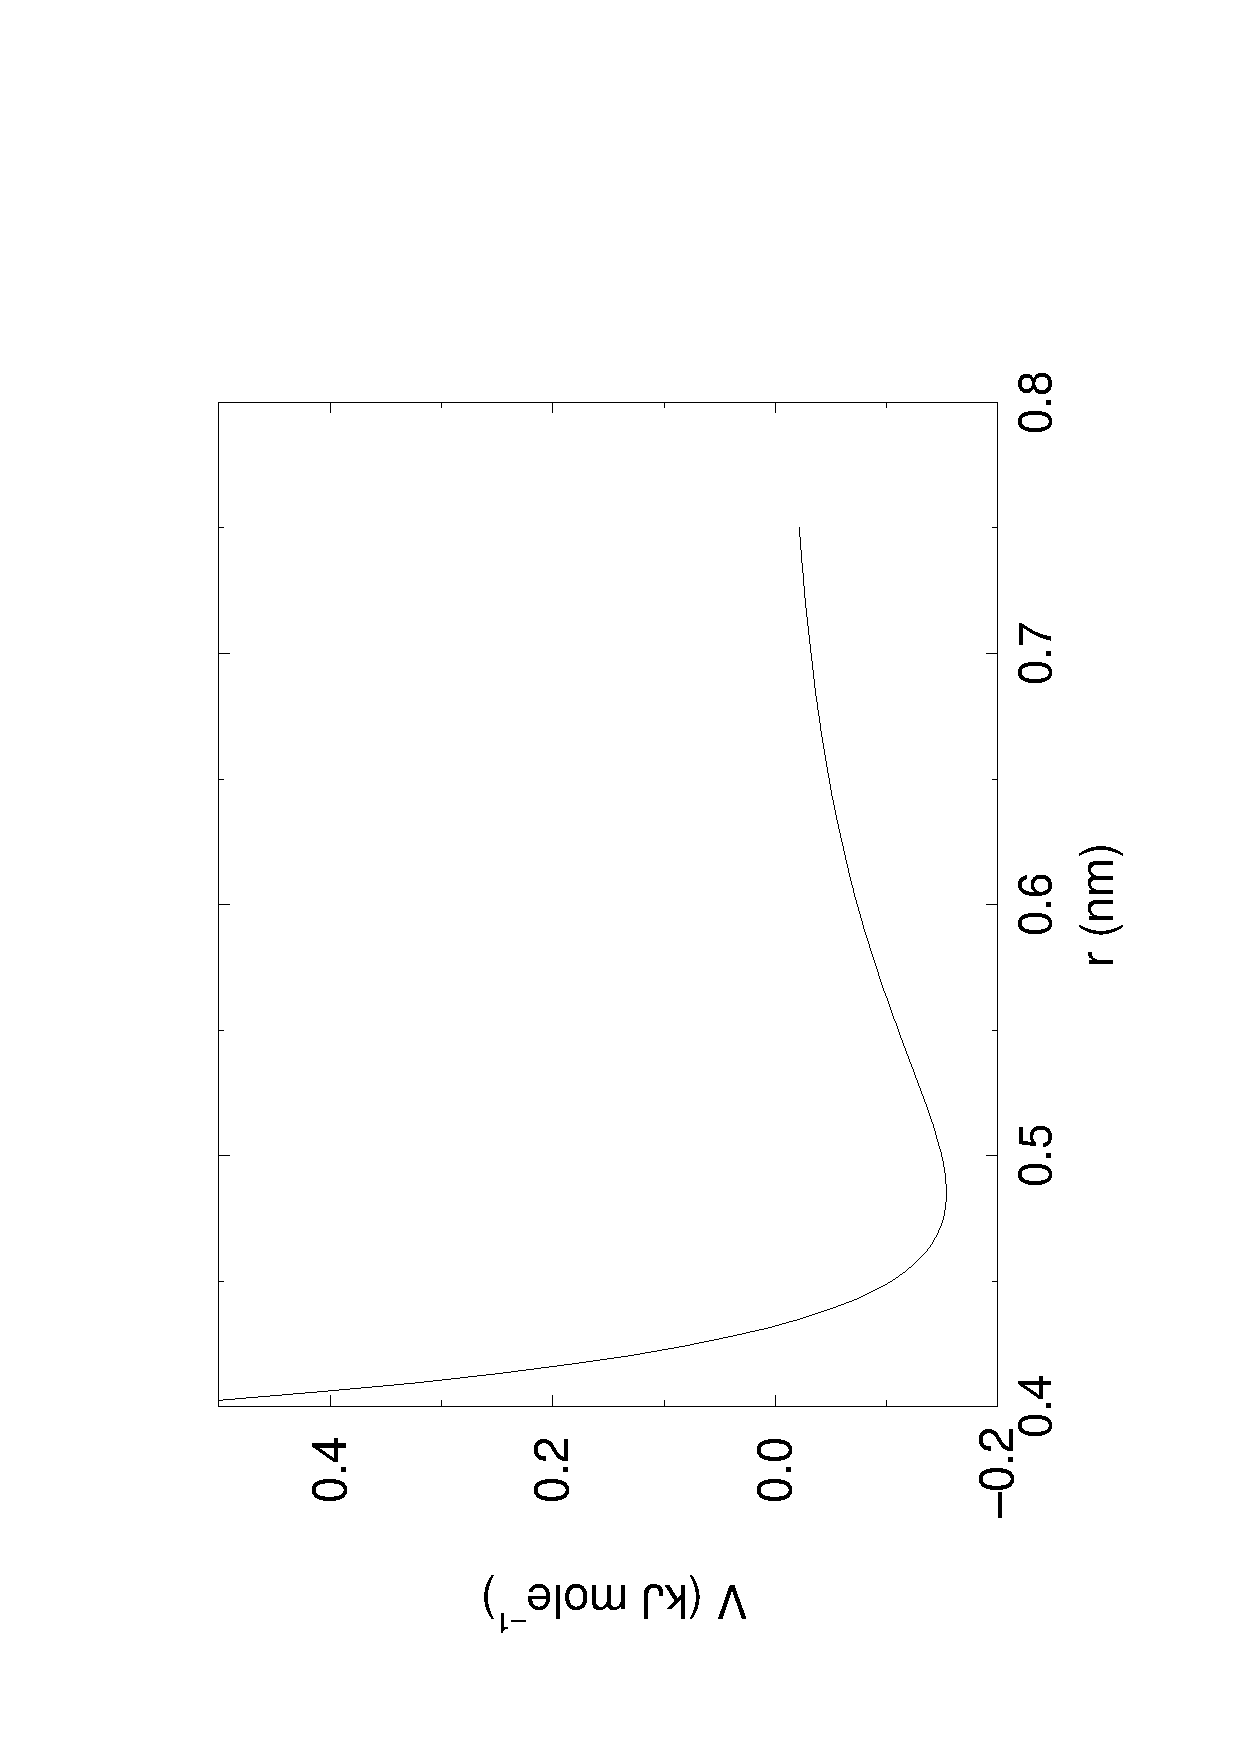
\includegraphics[width=8cm]{plots/f_lj}}
\caption {The Lennard-Jones interaction.}
\label{fig:lj}
\end{figure}
 
The force derived from this potential is:
\beq
\ve{F}_i(\rvij) = \left( 12~\frac{C_{ij}^{(12)}}{\rij^{13}} -
                                 6~\frac{C_{ij}^{(6)}}{\rij^7} \right) \rnorm 
\eeq

The LJ potential may also be written in the following form :
\beq
V_{LJ}(\rvij) = 4\epsilon_{ij}\left(\left(\frac{\sigma_{ij}} {\rij}\right)^{12}
                - \left(\frac{\sigma_{ij}}{\rij}\right)^{6} \right)
\label{eqn:sigeps}      
\eeq

In constructing the parameter matrix for the non-bonded LJ-parameters,
two types of \normindex{combination rule}s can be used within {\gromacs},
only geometric averages (type 1 in the input section of the force field file):
\beq
\begin{array}{rcl}
C_{ij}^{(6)}    &=& \left({C_{ii}^{(6)} \, C_{jj}^{(6)}}\right)^{1/2}    \\
C_{ij}^{(12)}   &=& \left({C_{ii}^{(12)} \, C_{jj}^{(12)}}\right)^{1/2}
\label{eqn:comb}
\end{array}
\eeq
or, alternatively the Lorentz-Bertelot rules can be used. An arithmetic average is used to calculate $\sigma_{ij}$, while a geometric average is used to calculate $\epsilon_{ij}$ (type 2):
\beq
\begin{array}{rcl}
 \sigma_{ij}   &=& \frac{1}{ 2}(\sigma_{ii} + \sigma_{jj})        \\
 \epsilon_{ij} &=& \left({\epsilon_{ii} \, \epsilon_{jj}}\right)^{1/2}
\end{array}
\eeq
finally an geometric average for both parameters can be used (type 3):
\beq
\begin{array}{rcl}
 \sigma_{ij}   &=& \left({\sigma_{ii} \, \sigma_{jj}}\right)^{1/2}        \\
 \epsilon_{ij} &=& \left({\epsilon_{ii} \, \epsilon_{jj}}\right)^{1/2}
\end{array}
\eeq
this last rule is used by the OPLS force field.


\ifthenelse{\equal{\gmxlite}{1}}{}{
\subsection{Buckingham potential}
The \normindex{Buckingham} 
potential has a more flexible and realistic repulsion term
than the Lennard-Jones interaction, but is also more expensive to
compute. The potential form is:
\beq
V_{bh}(\rij) = A_{ij} \exp(-B_{ij} \rij) -
                        \frac{C_{ij}}{\rij^6}
\eeq
\begin{figure}
\centerline{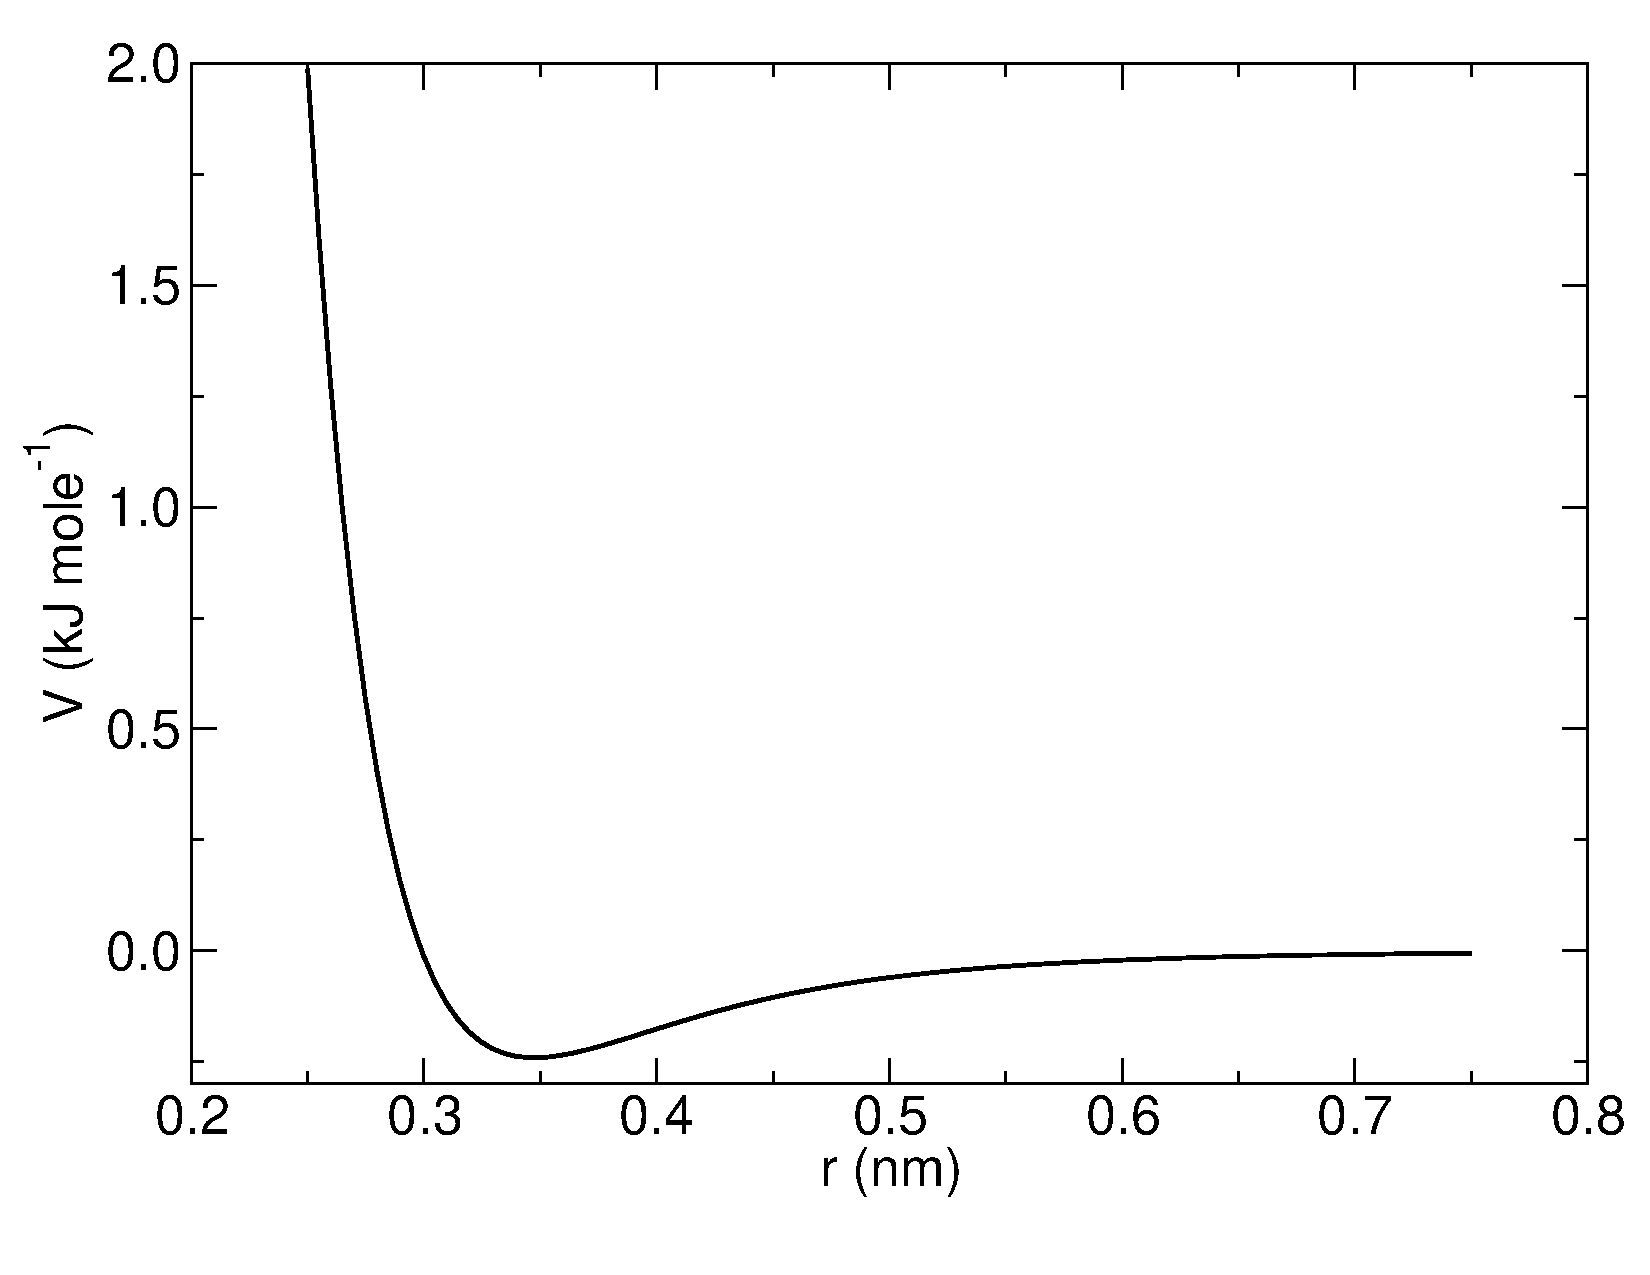
\includegraphics[width=8cm]{plots/f_bham}}
\caption {The Buckingham interaction.}
\label{fig:bham}
\end{figure}

see also \figref{bham}, the force derived from this is:
\beq
 \ve{F}_i(\rij) = \left[ A_{ij}B_{ij}\exp(-B_{ij} \rij) -
                                 6\frac{C_{ij}}{\rij^7} \right] \rnorm
\eeq

There is only one set of \normindex{combination rule}s
for Buckingham potentials:
\beq
\begin{array}{rcl}
A_{ij}   &=& \left(A_{ii} \, A_{jj}\right)^{1/2}    \\
B_{ij}   &=& \frac{1}{ 2}(B_{ii} + B_{jj})        \\
C_{ij}   &=& \left(C_{ii} \, C_{jj}\right)^{1/2}
\end{array}
\eeq
} % Brace matches ifthenelse test for gmxlite

\subsection{Coulomb interaction}
\label{sec:coul}
\newcommand{\epsr}{\varepsilon_r}
\newcommand{\epsrf}{\varepsilon_{rf}}
The \normindex{Coulomb} interaction between two charge particles is given by:
\beq
V_c(\rij) = f \frac{q_i q_j}{\epsr \rij}
\label{eqn:vcoul}
\eeq
see also \figref{coul}, where $f = \frac{1}{4\pi \varepsilon_0} =
138.935\,485$ (see \chref{defunits})

\begin{figure}
\centerline{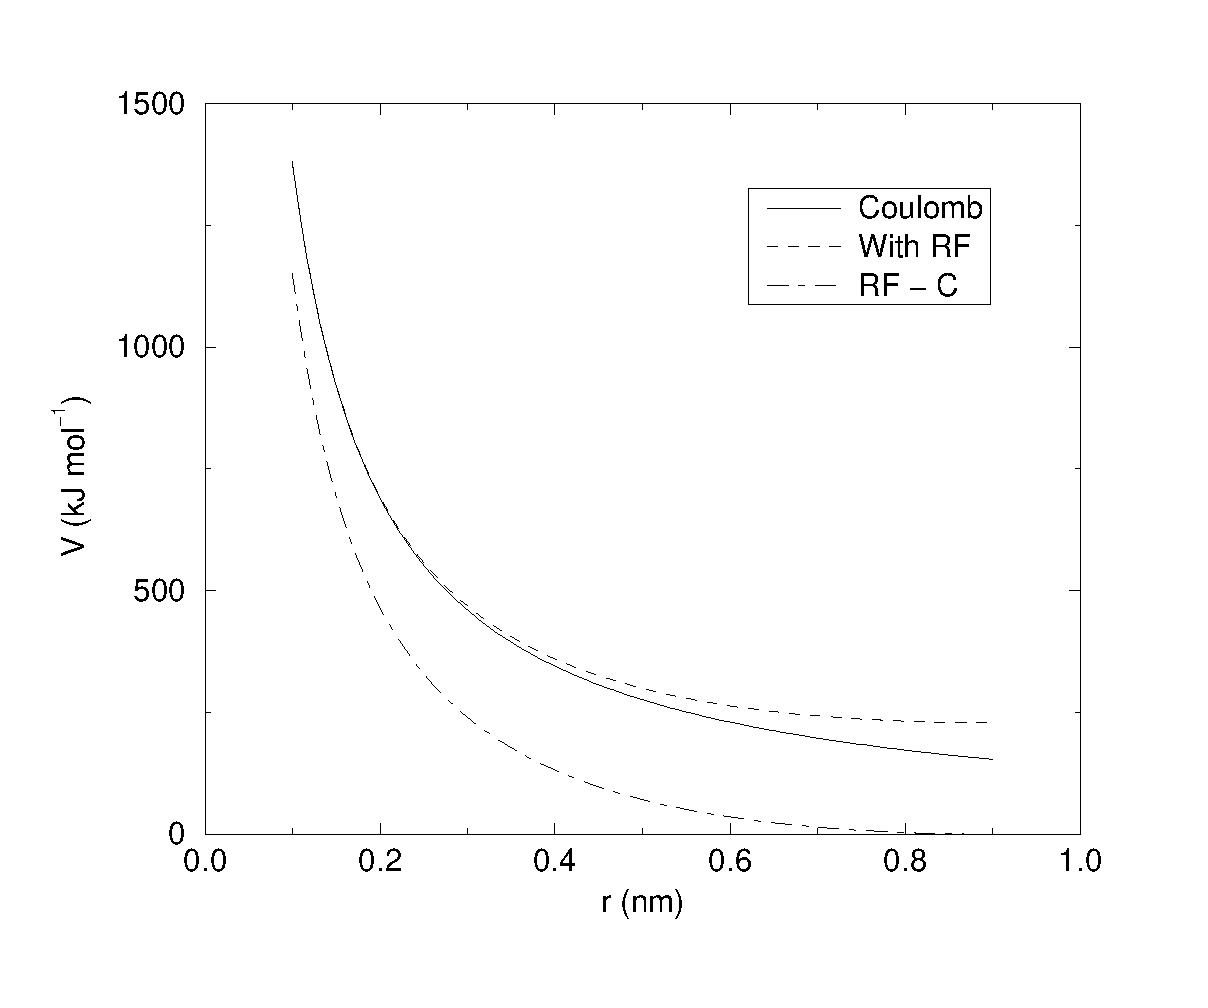
\includegraphics[width=8cm]{plots/vcrf}}
\caption[The Coulomb interaction with and without reaction field.]{The
Coulomb interaction (for particles with equal signed charge) with and
without reaction field. In the latter case $\epsr$ was 1, $\epsrf$ was 78,
and $r_c$ was 0.9 nm.
The dot-dashed line is the same as the dashed line, except for a constant.}
\label{fig:coul}
\end{figure}

The force derived from this potential is:
\beq
\ve{F}_i(\rvij) = f \frac{q_i q_j}{\epsr\rij^2}\rnorm
\eeq

In {\gromacs} the  relative \swapindex{dielectric}{constant} 
\normindex{$\epsr$}
may be set in the in the input for {\tt grompp}. 

\ifthenelse{\equal{\gmxlite}{1}}{}{
\subsection{Coulomb interaction with \normindex{reaction field}}
\label{sec:coulrf}
The coulomb interaction can be modified for homogeneous systems, by
assuming a constant dielectric environment beyond the cut-off $r_c$
with a dielectric constant of {$\epsrf$}. The interaction then reads:
\beq
V_{crf} ~=~
  f \frac{q_i q_j}{\epsr\rij}\left[1+\frac{\epsrf-\epsr}{2\epsrf+\epsr}
  \,\frac{\rij^3}{r_c^3}\right]
  - f\frac{q_i q_j}{\epsr r_c}\,\frac{3\epsrf}{2\epsrf+\epsr}
\label{eqn:vcrf}
\eeq
in which the constant expression on the right makes the potential
zero at the cut-off $r_c$. For charged cut-off spheres this corresponds
to neutralization with a homogeneous background charge.
We can rewrite \eqnref{vcrf} for simplicity as
\beq
V_{crf} ~=~     f \frac{q_i q_j}{\epsr}\left[\frac{1}{\rij} + k_{rf}~ \rij^2 -c_{rf}\right]
\eeq
with
\bea
k_{rf}  &=&     \frac{1}{r_c^3}\,\frac{\epsrf-\epsr}{(2\epsrf+\epsr)}   \label{eqn:krf}\\
c_{rf}  &=&     \frac{1}{r_c}+k_{rf}\,r_c^2 ~=~ \frac{1}{r_c}\,\frac{3\epsrf}{(2\epsrf+\epsr)}
\label{eqn:crf}
\eea
For large $\epsrf$ the $k_{rf}$ goes to $r_c^{-3}/2$,
while for $\epsrf$ = $\epsr$ the correction vanishes.
In \figref{coul}
the modified interaction is plotted, and it is clear that the derivative 
with respect to $\rij$ (= -force) goes to zero at the cut-off distance.
The force derived from this potential reads:
\beq
\ve{F}_i(\rvij) = f \frac{q_i q_j}{\epsr}\left[\frac{1}{\rij^2} - 2 k_{rf}\rij\right]\rnorm
\label{eqn:fcrf}
\eeq
The reaction-field correction should also be applied to all excluded
atoms pairs, including self pairs, in which case the normal Coulomb
term in \eqnsref{vcrf}{fcrf} is absent.

Tironi {\etal} have introduced a generalized reaction field in which
the dielectric continuum beyond the cut-off $r_c$ also has an ionic strength
$I$~\cite{Tironi95}. In this case we can rewrite the constants $k_{rf}$ and 
$c_{rf}$ using the inverse Debye screening length $\kappa$:
\bea
\kappa^2  &=&     
   \frac{2 I \,F^2}{\varepsilon_0 \epsrf RT}
   = \frac{F^2}{\varepsilon_0 \epsrf RT}\sum_{i=1}^{K} c_i z_i^2     \\
k_{rf}  &=&     \frac{1}{r_c^3}\,
    \frac{(\epsrf-\epsr)(1 + \kappa r_c) + \half\epsrf(\kappa r_c)^2}
         {(2\epsrf + \epsr)(1 + \kappa r_c) + \epsrf(\kappa r_c)^2}
    \label{eqn:kgrf}\\
c_{rf}  &=&     \frac{1}{r_c}\,
    \frac{3\epsrf(1 + \kappa r_c + \half(\kappa r_c)^2)}
         {(2\epsrf+\epsr)(1 + \kappa r_c) + \epsrf(\kappa r_c)^2}
    \label{eqn:cgrf}
\eea
where $F$ is Faraday's constant, $R$ is the ideal gas constant, $T$
the absolute temperature, $c_i$ the molar concentration for species
$i$ and $z_i$ the charge number of species $i$ where we have $K$
different species. In the limit of zero ionic strength ($\kappa=0$)
\eqnsref{kgrf}{cgrf} reduce to the simple forms of \eqnsref{krf}{crf}
respectively.

\subsection{Modified non-bonded interactions}
\label{sec:mod_nb_int}
In the {\gromacs} force field the non-bonded potentials can be
modified by a shift function. The purpose of this is to replace the
truncated forces by forces that are continuous and have continuous
derivatives at the \normindex{cut-off} radius. With such forces the
time-step integration produces much smaller errors and there are no
such complications as creating charges from dipoles by the truncation
procedure. In fact, by using shifted forces there is no need for
charge groups in the construction of neighbor lists. However, the
shift function produces a considerable modification of the Coulomb
potential. Unless the 'missing' long-range potential is properly
calculated and added (through the use of PPPM, Ewald, or PME), the
effect of such modifications must be carefully evaluated.  The
modification of the Lennard-Jones dispersion and repulsion is only
minor, but it does remove the noise caused by cut-off effects.
 
There is {\em no} fundamental difference between a switch function
(which multiplies the potential with a function) and a shift function
(which adds a function to the force or potential)~\cite{Spoel2006a}. The switch
function is a special case of the shift function, which we apply to
the {\em force function} $F(r)$, related to the electrostatic or
van der Waals force acting on particle $i$ by particle $j$ as
\beq
\ve{F}_i = c F(r_{ij}) \frac{\rvij}{r_{ij}}
\eeq
For pure Coulomb or Lennard-Jones interactions
$F(r)=F_\alpha(r)=r^{-(\alpha+1)}$.
The shifted force $F_s(r)$ can generally be written as:
\beq
\begin{array}{rcl}
\vspace{2mm}
F_s(r)~=&~F_\alpha(r)   & r < r_1               \\
\vspace{2mm}
F_s(r)~=&~F_\alpha(r)+S(r)      & r_1 \le r < r_c       \\
F_s(r)~=&~0             & r_c \le r     
\end{array}
\eeq
When $r_1=0$ this is a traditional shift function, otherwise it acts as a 
switch function. The corresponding shifted coulomb potential then reads:
\beq
V_s(r_{ij}) = f \Phi_s (r_{ij}) q_i q_j
\eeq
where $\Phi(r)$ is the potential function 
\beq
\Phi_s(r) =  \int^{\infty}_r~F_s(x)\, dx
\eeq

The {\gromacs} shift function should be smooth at the boundaries, therefore
the following boundary conditions are imposed on the shift function:
\beq
\begin{array}{rcl}
S(r_1)          &=&0            \\
S'(r_1)         &=&0            \\
S(r_c)          &=&-F_\alpha(r_c)       \\
S'(r_c)         &=&-F_\alpha'(r_c)
\end{array}
\eeq
A 3$^{rd}$ degree polynomial of the form
\beq
S(r) = A(r-r_1)^2 + B(r-r_1)^3
\eeq
fulfills these requirements. The constants A and B are given by the
boundary condition at $r_c$: 
\beq
\begin{array}{rcl}
\vspace{2mm}
A &~=~& -\displaystyle
        \frac{(\alpha+4)r_c~-~(\alpha+1)r_1} {r_c^{\alpha+2}~(r_c-r_1)^2} \\
B &~=~& \displaystyle
        \frac{(\alpha+3)r_c~-~(\alpha+1)r_1}{r_c^{\alpha+2}~(r_c-r_1)^3}
\end{array}
\eeq
Thus the total force function is
\beq
F_s(r) = \frac{\alpha}{r^{\alpha+1}} + A(r-r_1)^2 + B(r-r_1)^3
\eeq
and the potential function reads
\beq
\Phi(r) = \frac{1}{r^\alpha} - \frac{A}{3} (r-r_1)^3 - \frac{B}{4} (r-r_1)^4 - C
\eeq
where 
\beq
C =  \frac{1}{r_c^\alpha} - \frac{A}{3} (r_c-r_1)^3 - \frac{B}{4} (r_c-r_1)^4
\eeq

When $r_1$ = 0, the modified Coulomb force function is
\beq
 F_s(r) = \frac{1}{r^2} - \frac{5 r^2}{r_c^4} + \frac{4 r^3}{r_c^5}
\eeq
identical to the {\em \swapindex{parabolic}{force}} 
function recommended to be used as a short-range function in 
conjunction with a \swapindex{Poisson}{solver} 
for the long-range part~\cite{Berendsen93a}.
The modified Coulomb potential function is
\beq
\Phi(r) = \frac{1}{r} - \frac{5}{3r_c} + \frac{5r^3}{3r_c^4} - \frac{r^4}{r_c^5}
\eeq
see also \figref{shift}.

\begin{figure}
\centerline{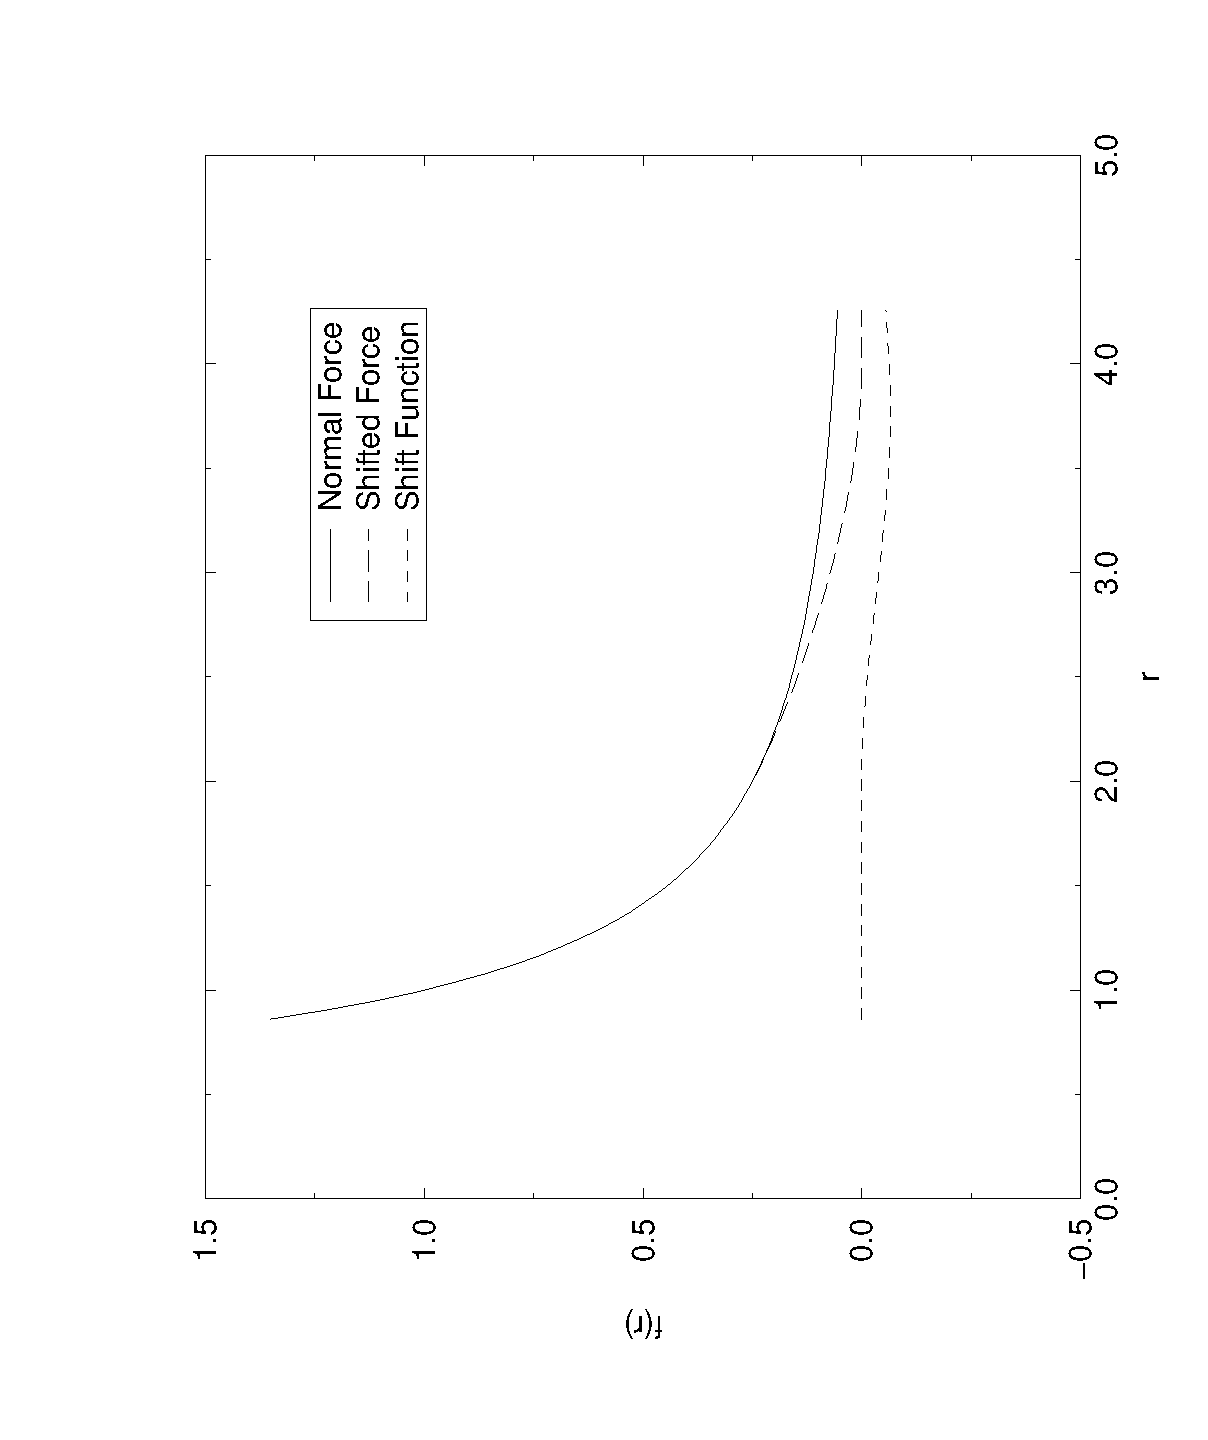
\includegraphics[angle=270,width=10cm]{plots/shiftf}}
\caption[The Coulomb Force, Shifted Force and Shift Function
$S(r)$,.]{The Coulomb Force, Shifted Force and Shift Function $S(r)$,
using r$_1$ = 2 and r$_c$ = 4.} 
\label{fig:shift}
\end{figure}

\subsection{Modified short-range interactions with Ewald summation}
When \normindex{Ewald sum}mation or \seeindex{particle-mesh
Ewald}{PME}\index{Ewald, particle-mesh} is used to calculate the
long-range interactions, the 
short-range coulomb potential must also be modified, similar to the
switch function above. In this case the short range potential is given
by
\beq
V(r) = f \frac{\mbox{erfc}(\beta r_{ij})}{r_{ij}} q_i q_j,
\eeq
where $\beta$ is a parameter that determines the relative weight 
between the direct space sum and the reciprocal space sum and erfc$(x)$ is
the complementary error function. For further 
details on long-range electrostatics, see \secref{lr_elstat}.
} % Brace matches ifthenelse test for gmxlite


\section{Bonded interactions}
Bonded interactions are based on a fixed list of atoms. They are not
exclusively pair interactions, but include 3- and 4-body interactions
as well. There are {\em bond stretching} (2-body), {\em bond angle}
(3-body), and {\em dihedral angle} (4-body) interactions. A special
type of dihedral interaction (called {\em improper dihedral}) is used
to force atoms to remain in a plane or to prevent transition to a
configuration of opposite chirality (a mirror image).

\subsection{Bond stretching}
\label{sec:bondpot}
\subsubsection{Harmonic potential}
The \swapindex{bond}{stretching} between two covalently bonded atoms
$i$ and $j$ is represented by a harmonic potential

\begin{figure}
\centerline{\raisebox{4cm}{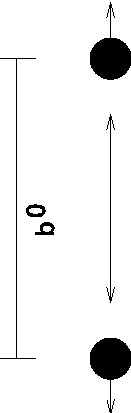
\includegraphics[angle=270,width=5cm]{plots/bstretch}}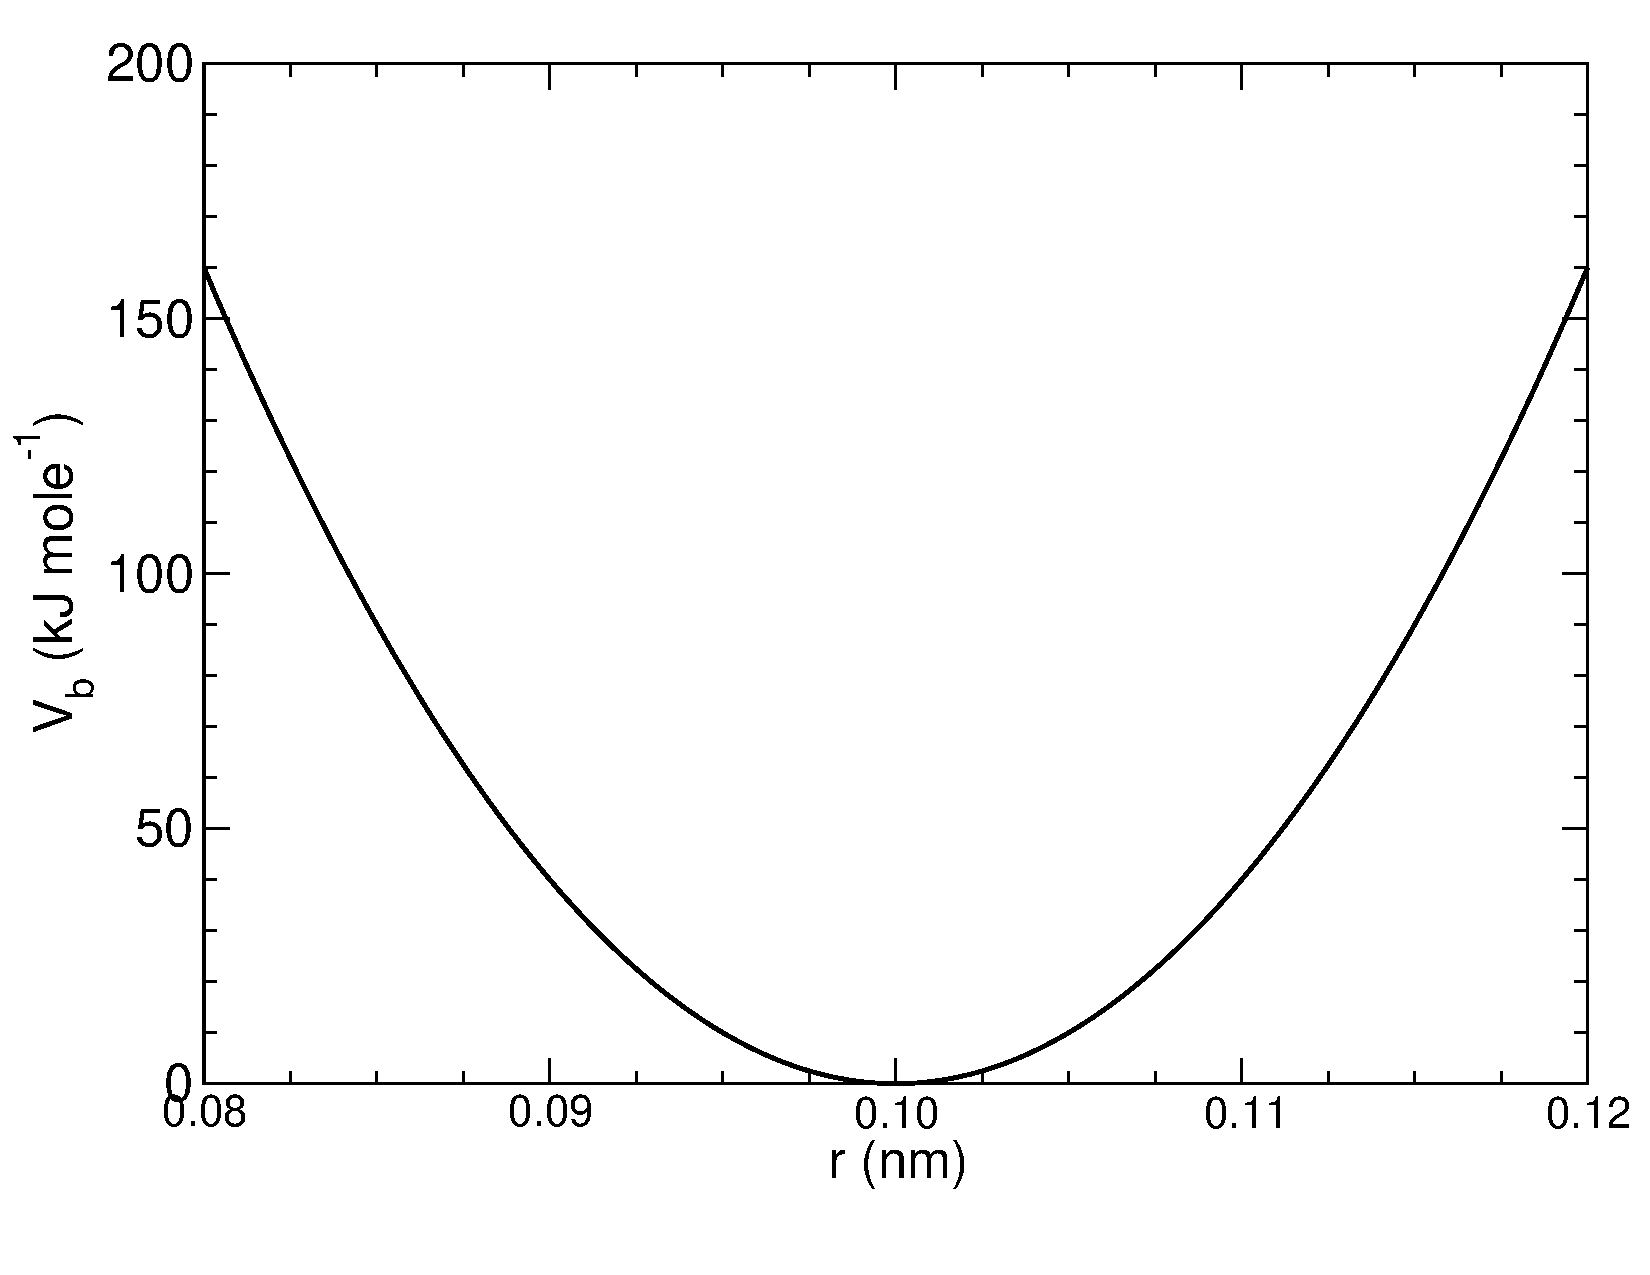
\includegraphics[width=7cm]{plots/f_bond}}
\caption[Bond stretching.]{Principle of bond stretching (left), and the bond
stretching potential (right).}
\label{fig:bstretch1}
\end{figure}

\beq
V_b~(\rij) = \half k^b_{ij}(\rij-b_{ij})^2
\eeq
see also \figref{bstretch1}, with the force
\beq
\ve{F}_i(\rvij) = k^b_{ij}(\rij-b_{ij}) \rnorm
\eeq

\ifthenelse{\equal{\gmxlite}{1}}{}{
\subsubsection{Fourth power potential}
In the \gromosv{96} force field~\cite{gromos96} the covalent bond potential
is written for reasons of computational efficiency as:
\beq
V_b~(\rij) = \frac{1}{4}k^b_{ij}\left(\rij^2-b_{ij}^2\right)^2
\eeq
the corresponding  force is:
\beq
\ve{F}_i(\rvij) = k^b_{ij}(\rij^2-b_{ij}^2)~\rvij
\eeq
The force constants for this form of the potential is related to the usual
harmonic force constant $k^{b,harm}$ (\secref{bondpot}) as
\beq
2 k^b b_{ij}^2 = k^{b,harm}
\eeq
The force constants are mostly derived from the harmonic ones used in 
\gromosv{87}~\cite{biomos}. Although this form is computationally more 
efficient
(because no square root has to be evaluated), it is conceptually more
complex. One particular disadvantage is that since the form is not harmonic,
the average energy of a single bond is not equal to $\half kT$ as it is for 
the normal harmonic potential.

\subsection{Morse potential bond stretching}
%\author{F.P.X. Everdij}
%
For some systems that require an anharmonic bond stretching potential,
the Morse potential~\cite{Morse29} 
between two atoms {\it i} and {\it j} is available
in {\gromacs}. This potential differs from the harmonic potential in
having an asymmetric potential well and a zero force at infinite
distance. The functional form is:
\beq
\displaystyle V_{morse} (r_{ij}) = D_{ij} [1 - \exp(-\beta_{ij}(r_{ij}-b_{ij}))]^2,
\eeq
see also \figref{morse}, and the corresponding force is:
\beq
\begin{array}{rcl}
\displaystyle {\bf F}_{morse} ({\bf r}_{ij})&=&2 D_{ij} \beta_{ij} r_{ij} \exp(-\beta_{ij}(r_{ij}-b_{ij})) * \\
\displaystyle \: & \: &[1 - \exp(-\beta_{ij}(r_{ij}-b_{ij}))] \frac{\displaystyle {\bf r}_{ij}}{\displaystyle r_{ij}},
\end{array}
\eeq
where \( \displaystyle D_{ij} \) is the depth of the well in kJ/mol,
\( \displaystyle \beta_{ij} \) defines the steepness of the well (in
nm\(^{-1} \)), and \( \displaystyle b_{ij} \) is the equilibrium
distance in nm.  The steepness parameter \( \displaystyle \beta_{ij}
\) can be expressed in terms of the reduced mass of the atoms {\it i}
and {\it j}, the fundamental vibration frequency \( \displaystyle
\omega_{ij} \) and the well depth \( \displaystyle D_{ij} \):
\beq
\displaystyle \beta_{ij}= \omega_{ij} \sqrt{\frac{\mu_{ij}}{2 D_{ij}}}
\eeq
and because \( \displaystyle \omega = \sqrt{k/\mu} \), one can rewrite \( \displaystyle \beta_{ij} \) in terms of the harmonic force constant \( \displaystyle k_{ij} \)
\beq
\displaystyle \beta_{ij}= \sqrt{\frac{k_{ij}}{2 D_{ij}}}
\label{eqn:betaij}
\eeq
For small deviations \( \displaystyle (r_{ij}-b_{ij}) \), one can
approximate the \( \displaystyle \exp \)-term to first-order using a
Taylor expansion:
\beq
\displaystyle \exp(-x) \approx 1-x
\label{eqn:expminx}
\eeq
and substituting \eqnref{betaij} and \eqnref{expminx} in the functional from,
\beq
\begin{array}{rcl}
\displaystyle V_{morse} (r_{ij})&=&D_{ij} [1 - \exp(-\beta_{ij}(r_{ij}-b_{ij}))]^2\\
\displaystyle \:&=&D_{ij} [1 - (1 -\sqrt{\frac{k_{ij}}{2 D_{ij}}}(r_{ij}-b_{ij}))]^2\\
\displaystyle \:&=&\frac{1}{2} k_{ij} (r_{ij}-b_{ij}))^2,
\end{array}
\eeq
we recover the harmonic bond stretching potential.

\begin{figure}
\centerline{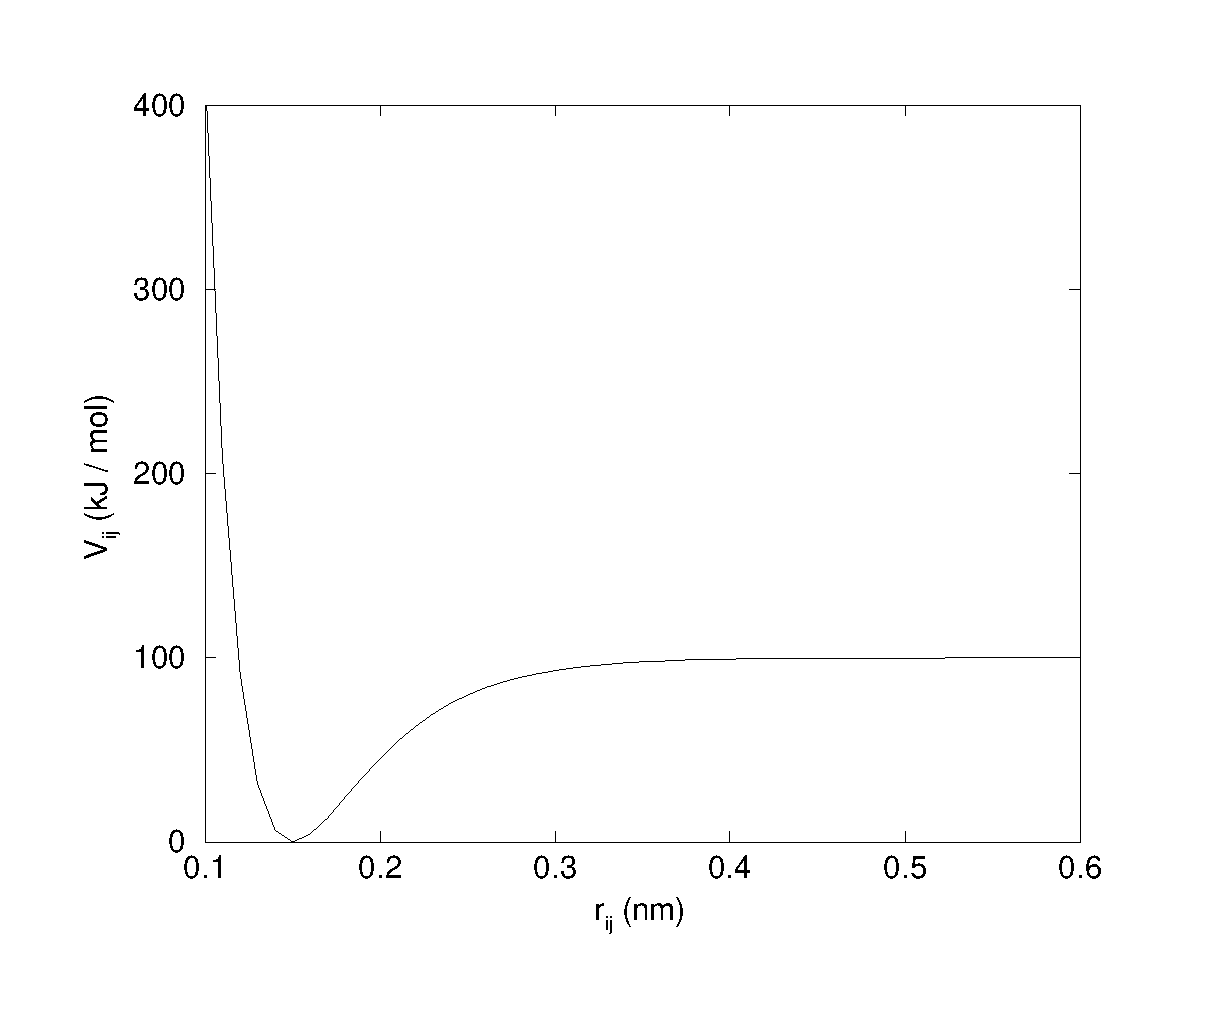
\includegraphics[width=7cm]{plots/f_morse}}
\caption{The Morse potential well, with bond length 0.15 nm.}
\label{fig:morse}
\end{figure}

\subsection{Cubic bond stretching potential}
Another anharmonic bond stretching potential that is slightly simpler
than the Morse potential adds a cubic term in the distance to the
simple harmonic form:
\beq
V_b~(\rij) = k^b_{ij}(\rij-b_{ij})^2 + k^b_{ij}k^{cub}_{ij}(\rij-b_{ij})^3
\eeq
A flexible \normindex{water} model (based on
the SPC water model~\cite{Berendsen81}) including 
a cubic bond stretching potential for the O-H bond
was developed by Ferguson~\cite{Ferguson95}. This model was found
to yield a reasonable infrared spectrum. The Ferguson water model is
available in the {\gromacs} library. 
It should be noted that the potential is asymmetric: overstretching leads to
infinitely low energies. The \swapindex{integration}{timestep} is therefore
limited to 1 fs.

The force corresponding to this potential is:
\beq
\ve{F}_i(\rvij) = 2k^b_{ij}(\rij-b_{ij})~\rnorm + 3k^b_{ij}k^{cub}_{ij}(\rij-b_{ij})^2~\rnorm
\eeq

\subsection{FENE bond stretching potential}
\index{FENE potential}
In coarse-grained polymer simulations the beads are often connected
by a FENE (finitely extensible nonlinear elastic) potential~\cite{Warner72}:
\beq
V_{\mbox{\small FENE}}(\rij) =
  -\half k^b_{ij} b^2_{ij} \log\left(1 - \frac{\rij^2}{b^2_{ij}}\right)
\eeq
The potential looks complicated, but the expression for the force is simpler:
\beq
F_{\mbox{\small FENE}}(\rvij) =
  -k^b_{ij} \left(1 - \frac{\rij^2}{b^2_{ij}}\right)^{-1} \rvij
\eeq
At short distances the potential asymptotically goes to a harmonic
potential with force constant $k^b$, while it diverges at distance $b$.
} % Brace matches ifthenelse test for gmxlite

\subsection{Harmonic angle potential}
\label{sec:anglepot}
\newcommand{\tijk}{\theta_{ijk}}
The bond \swapindex{angle}{vibration} between a triplet of atoms $i$ - $j$ - $k$
is also represented by a harmonic potential on the angle $\tijk$

\begin{figure}
\centerline{\raisebox{4cm}{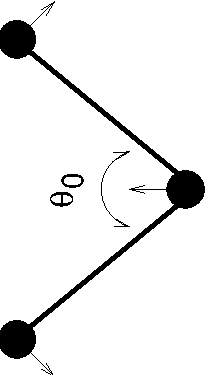
\includegraphics[angle=270,width=5cm]{plots/angle}}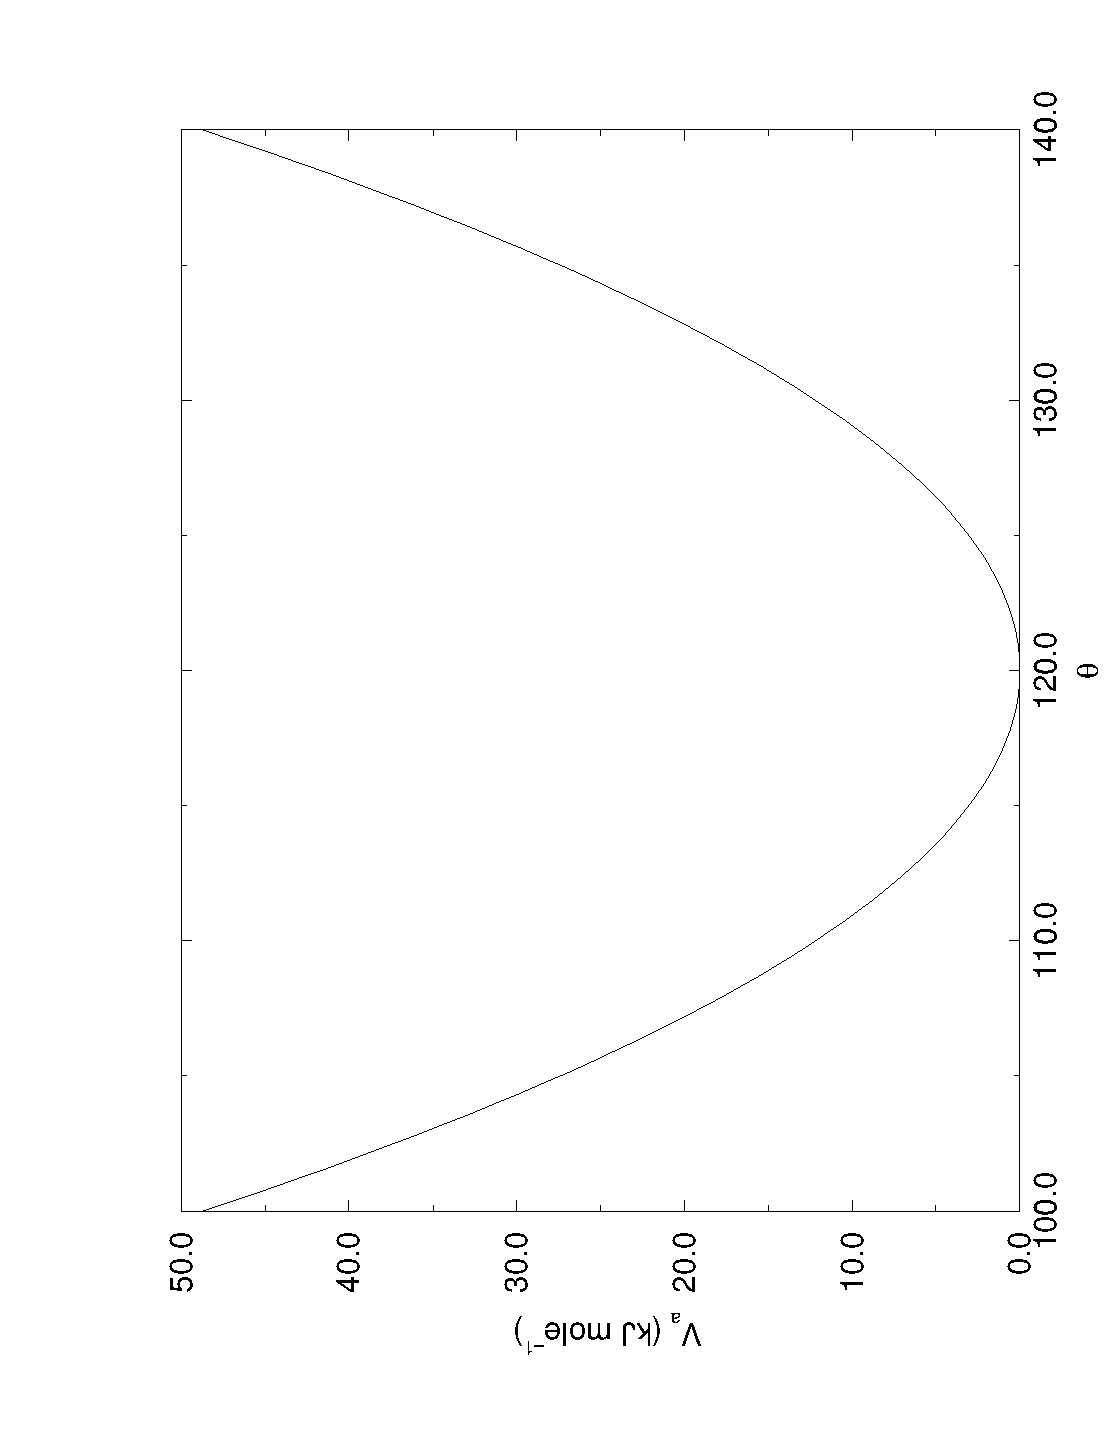
\includegraphics[width=7cm]{plots/f_angle}}
\caption[Angle vibration.]{Principle of angle vibration (left) and the
bond angle potential (right).}
\label{fig:angle}
\end{figure}

\beq
V_a(\tijk) = \half k^{\theta}_{ijk}(\tijk-\tijk^0)^2
\eeq
As the bond-angle vibration is represented by a harmonic potential, the
form is the same as the bond stretching (\figref{bstretch1}).

The force equations are given by the chain rule:
\beq
\begin{array}{l}
\Fvi    ~=~ -\displaystyle\frac{d V_a(\tijk)}{d \rvi}   \\
\Fvk    ~=~ -\displaystyle\frac{d V_a(\tijk)}{d \rvk}   \\
\Fvj    ~=~ -\Fvi-\Fvk
\end{array}
~ \mbox{ ~ where ~ } ~
 \tijk = \arccos \frac{(\rvij \cdot \ve{r}_{kj})}{r_{ij}r_{kj}}
\eeq
The numbering $i,j,k$ is in sequence of covalently bonded atoms. Atom
$j$ is in the middle; atoms $i$  and $k$ are at the ends (see \figref{angle}).
{\bf Note} that in the input in topology files, angles are given in degrees and
force constants in kJ/mol/rad$^2$.

\ifthenelse{\equal{\gmxlite}{1}}{}{
\subsection{Cosine based angle potential}
\label{sec:cosangle}
In the \gromosv{96} force field a simplified function is used to represent angle
vibrations:
\beq
V_a(\tijk) = \half k^{\theta}_{ijk}\left(\cos(\tijk) - \cos(\tijk^0)\right)^2
\eeq
where 
\beq
\cos(\tijk) = \frac{\rvij\cdot\ve{r}_{kj}}{\rij r_{kj}}
\eeq
The corresponding force can be derived by partial differentiation with respect
to the atomic positions. The force constants in this function are related
to the force constants in the harmonic form $k^{\theta,harm}$
(\secref{anglepot}) by:
\beq
k^{\theta} \sin^2(\tijk^0) = k^{\theta,harm}
\eeq
In the \gromosv{96} manual there is a much more complicated conversion formula
which is temperature dependent. The formulas are equivalent at 0 K
and the differences at 300 K are on the order of 0.1 to 0.2\%.
{\bf Note} that in the input in topology files, angles are given in degrees and
force constants in kJ/mol.

\subsection{Urey-Bradley potential}
\label{sec:urey-bradley}
The bond \swapindex{Urey-Bradley angle}{vibration} between a triplet
of atoms $i$ - $j$ - $k$ is represented by a harmonic potential on the
angle $\tijk$ and a harmonic correction term on the distance between
the atoms $i$ and $k$. Although this can be easily written as a simple
sum of two terms, it is convenient to have it as a single entry in the
topology file and in the output as a separate energy term. It is used mainly
in the CHARMm force field~\cite{BBrooks83}. The energy is given by:

\beq
V_a(\tijk) = \half k^{\theta}_{ijk}(\tijk-\tijk^0)^2 + \half k^{UB}_{ijk}(r_{ik}-r_{ik}^0)^2
\eeq

The force equations can be deduced from sections~\ref{sec:bondpot}
and~\ref{sec:anglepot}.

\subsection{Bond-Bond cross term}
The bond-bond cross term for three particles $i, j, k$ forming bonds
$i-j$ and $k-j$ is given by~\cite{Lawrence2003b}:
\begin{equation}
V_{rr'} ~=~ k_{rr'} \left(\left|\ve{r}_{i}-\ve{r}_j\right|-r_{1e}\right) \left(\left|\ve{r}_{k}-\ve{r}_j\right|-r_{2e}\right)
\label{crossbb}
\end{equation}
where $k_{rr'}$ is the force constant, and $r_{1e}$ and $r_{2e}$ are the
equilibrium bond lengths of the $i-j$ and $k-j$ bonds respectively. The force
associated with this potential on particle $i$ is:
\begin{equation}
\ve{F}_{i} = -k_{rr'}\left(\left|\ve{r}_{k}-\ve{r}_j\right|-r_{2e}\right)\frac{\ve{r}_i-\ve{r}_j}{\left|\ve{r}_{i}-\ve{r}_j\right|}
\end{equation}
the force on atom $k$ can be obtained by swapping $i$ and $k$ in the above
equation. Finally the force on atom $j$ follows from the fact that the sum
of internal forces should be zero: $\ve{F}_j = -\ve{F}_i-\ve{F}_k$.

\subsection{Bond-Angle cross term}
The bond-angle cross term for three particles $i, j, k$ forming bonds
$i-j$ and $k-j$ is given by~\cite{Lawrence2003b}:
\begin{equation}
V_{r\theta} ~=~ k_{r\theta} \left(\left|\ve{r}_{i}-\ve{r}_k\right|-r_{3e} \right) \left(\left|\ve{r}_{i}-\ve{r}_j\right|-r_{1e} + \left|\ve{r}_{k}-\ve{r}_j\right|-r_{2e}\right)
\end{equation}
where $k_{r\theta}$ is the force constant, $r_{3e}$ is the $i-k$ distance,
and the other constants are the same as in Equation~\ref{crossbb}. The force
associated with the potential on atom $i$ is:
\begin{equation}
\ve{F}_{i} ~=~ -k_{r\theta}\left[\left(\left|\ve{r}_{i}-\ve{r}_{k}\right|-r_{3e}\right)\frac{\ve{r}_i-\ve{r}_j}{\left|\ve{r}_{i}-\ve{r}_j\right|} \\
+ \left(\left|\ve{r}_{i}-\ve{r}_j\right|-r_{1e} + \left|\ve{r}_{k}-\ve{r}_j\right|-r_{2e}\right)\frac{\ve{r}_i-\ve{r}_k}{\left|\ve{r}_{i}-\ve{r}_k\right|}\right]
\end{equation}

\subsection{Quartic angle potential}
For special purposes there is an angle potential
that uses a fourth order polynomial:
\beq
V_q(\tijk) ~=~ \sum_{n=0}^5 C_n (\tijk-\tijk^0)^n
\eeq
} % Brace matches ifthenelse test for gmxlite

%% new commands %%%%%%%%%%%%%%%%%%%%%%
\newcommand{\rvkj}{{\bf r}_{kj}}
\newcommand{\rkj}{r_{kj}}
%%%%%%%%%%%%%%%%%%%%%%%%%%%%%%%%%%%%%%

\subsection{\swapindex{Improper}{dihedral}s}
\label{sec:imp}
Improper dihedrals are meant to keep \swapindex{planar}{group}s planar ({\eg} 
aromatic rings) or to prevent molecules from flipping over to their
\normindex{mirror image}s, see \figref{imp}.

\begin {figure}
\centerline{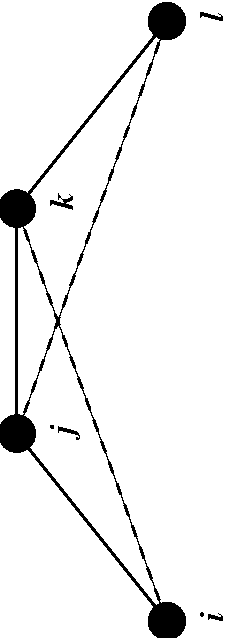
\includegraphics[angle=270,width=4cm]{plots/ring-imp}\hspace{1cm}
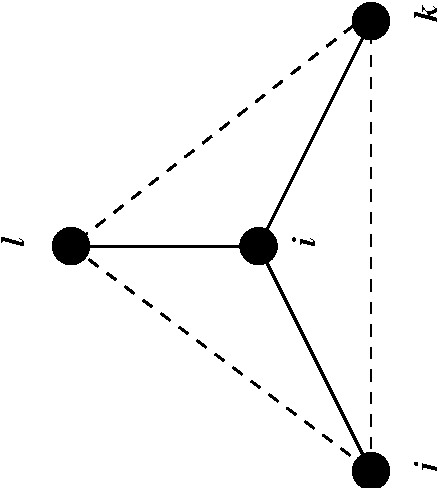
\includegraphics[angle=270,width=3cm]{plots/subst-im}\hspace{1cm}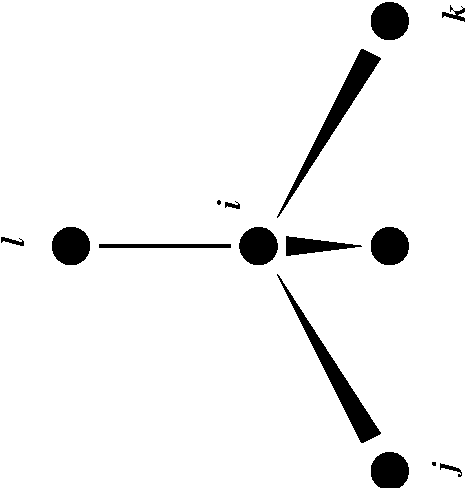
\includegraphics[angle=270,width=3cm]{plots/tetra-im}}
\caption[Improper dihedral angles.]{Principle of improper
dihedral angles. Out of plane bending for rings (left), substituents
of rings (middle), out of tetrahedral (right). The improper dihedral
angle $\xi$ is defined as the angle between planes (i,j,k) and (j,k,l)
in all cases.}
\label{fig:imp}
\end {figure}

\subsubsection{Improper dihedrals: harmonic type}
The simplest improper dihedral potential is a harmonic potential; it is plotted in
\figref{imps}.
\beq
V_{id}(\xi_{ijkl}) = \half k_{\xi}(\xi_{ijkl}-\xi_0)^2
\eeq
Since the potential is harmonic it is discontinuous,
but since the discontinuity is chosen at 180$^\circ$ distance from $\xi_0$
this will never cause problems.
{\bf Note} that in the input in topology files, angles are given in degrees and
force constants in kJ/mol/rad$^2$.

\begin{figure}
\centerline{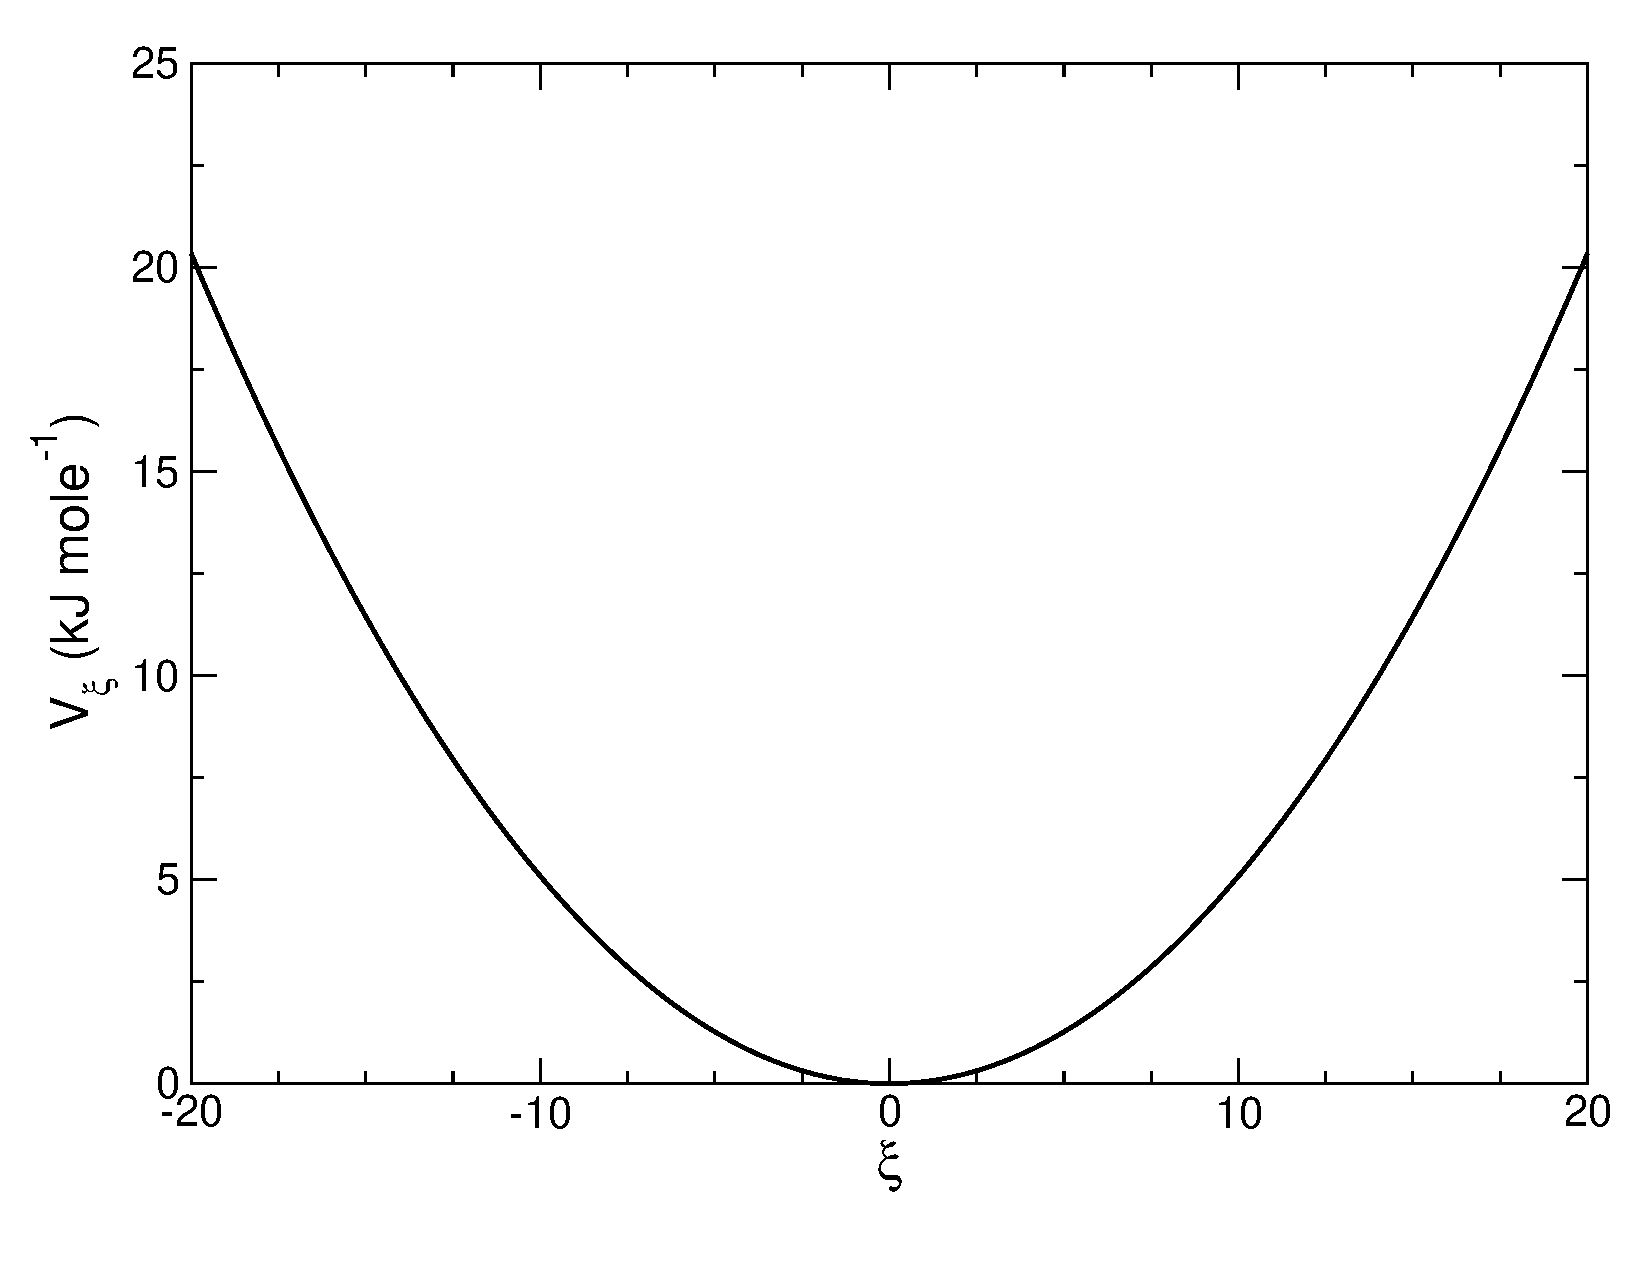
\includegraphics[width=8cm]{plots/f_imps}}
\caption{Improper dihedral potential.}
\label{fig:imps}
\end{figure}

\subsubsection{Improper dihedrals: periodic type}
This potential is identical to the periodic proper dihedral (see below).
There is a separate dihedral type for this (type 4) only to be able
to distinguish improper from proper dihedrals in the parameter section
and the output.

\subsection{Proper dihedrals}
For the normal \normindex{dihedral} interaction there is a choice of
either the {\gromos} periodic function or a function based on
expansion in powers of $\cos \phi$ (the so-called Ryckaert-Bellemans
potential). This choice has consequences for the inclusion of special
interactions between the first and the fourth atom of the dihedral
quadruple. With the periodic {\gromos} potential a special 1-4
LJ-interaction must be included; with the Ryckaert-Bellemans potential
{\em for alkanes} the \normindex{1-4 interaction}s must be excluded
from the non-bonded list.  {\bf Note:} Ryckaert-Bellemans potentials
are also used in e.g. the OPLS force field in combination with 1-4
interactions. You should therefore not modify topologies generated by
\normindex{pdb2gmx} in this case.

\subsubsection{Proper dihedrals: periodic type}
\swapindex{Proper}{dihedral} angles are defined according to the IUPAC/IUB
convention, where $\phi$ is the angle between the $ijk$ and the $jkl$
planes, with {\bf zero} corresponding to the {\em cis} configuration
($i$ and $l$ on the same side). There are two dihedral function types
in Gromacs topology files. There is the standard type 1 which behaves
like any other bonded interactions. For certain force fields type 9
is useful. Type 9 allows multiple potential functions to be applied
automatically to a single dihedral in the {\tt [ dihedral ]} section
when multiple parameters are defined for the same atomtypes
in the {\tt [ dihedraltypes ]} section.

\begin{figure}
\centerline{\raisebox{4.5cm}{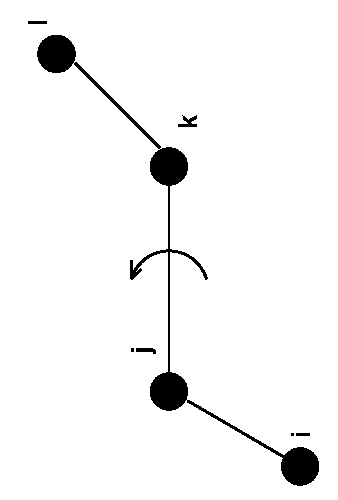
\includegraphics[angle=270,width=5cm]{plots/dih}}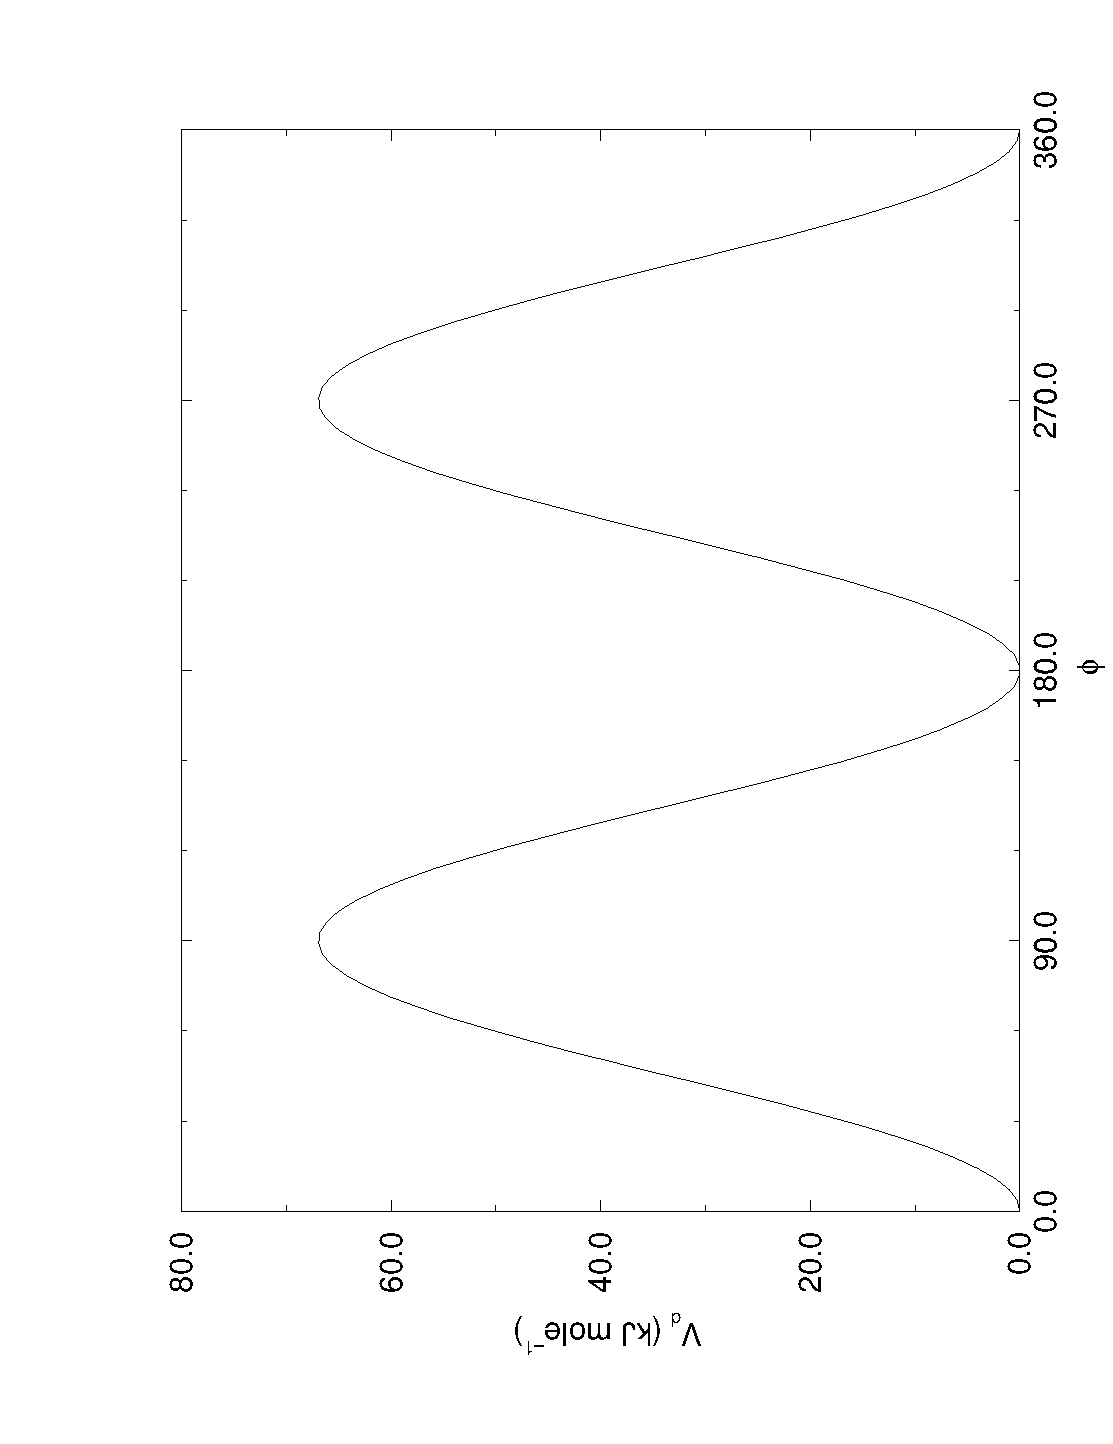
\includegraphics[width=7cm]{plots/f_dih}}
\caption[Proper dihedral angle.]{Principle of proper dihedral angle
(left, in {\em trans} form) and the dihedral angle potential (right).} 
\label{fig:pdihf}
\end{figure}
\beq
V_d(\phi_{ijkl}) = k_{\phi}(1 + \cos(n \phi - \phi_s))
\eeq

\ifthenelse{\equal{\gmxlite}{1}}{}{
\subsubsection{Proper dihedrals: Ryckaert-Bellemans function}
For alkanes, the following proper dihedral potential is often used
(see \figref{rbdih})
\beq
V_{rb}(\phi_{ijkl}) = \sum_{n=0}^5 C_n( \cos(\psi ))^n,
\eeq 
where $\psi = \phi - 180^\circ$.  \\
{\bf Note:} A conversion from one convention to another can be achieved by 
multiplying every coefficient \( \displaystyle C_n \) 
by \( \displaystyle (-1)^n \).

An example of constants for $C$ is given in \tabref{crb}.

\begin{table}
\centerline{
\begin{tabular}{|lr|lr|lr|}
\dline
$C_0$   & 9.28  & $C_2$   & -13.12  & $C_4$   & 26.24   \\
$C_1$   & 12.16 & $C_3$   & -3.06   & $C_5$   & -31.5   \\
\dline
\end{tabular}
}
\caption{Constants for Ryckaert-Bellemans potential (kJ mol$^{-1}$).}
\label{tab:crb}
\end{table}

\begin{figure}
\centerline{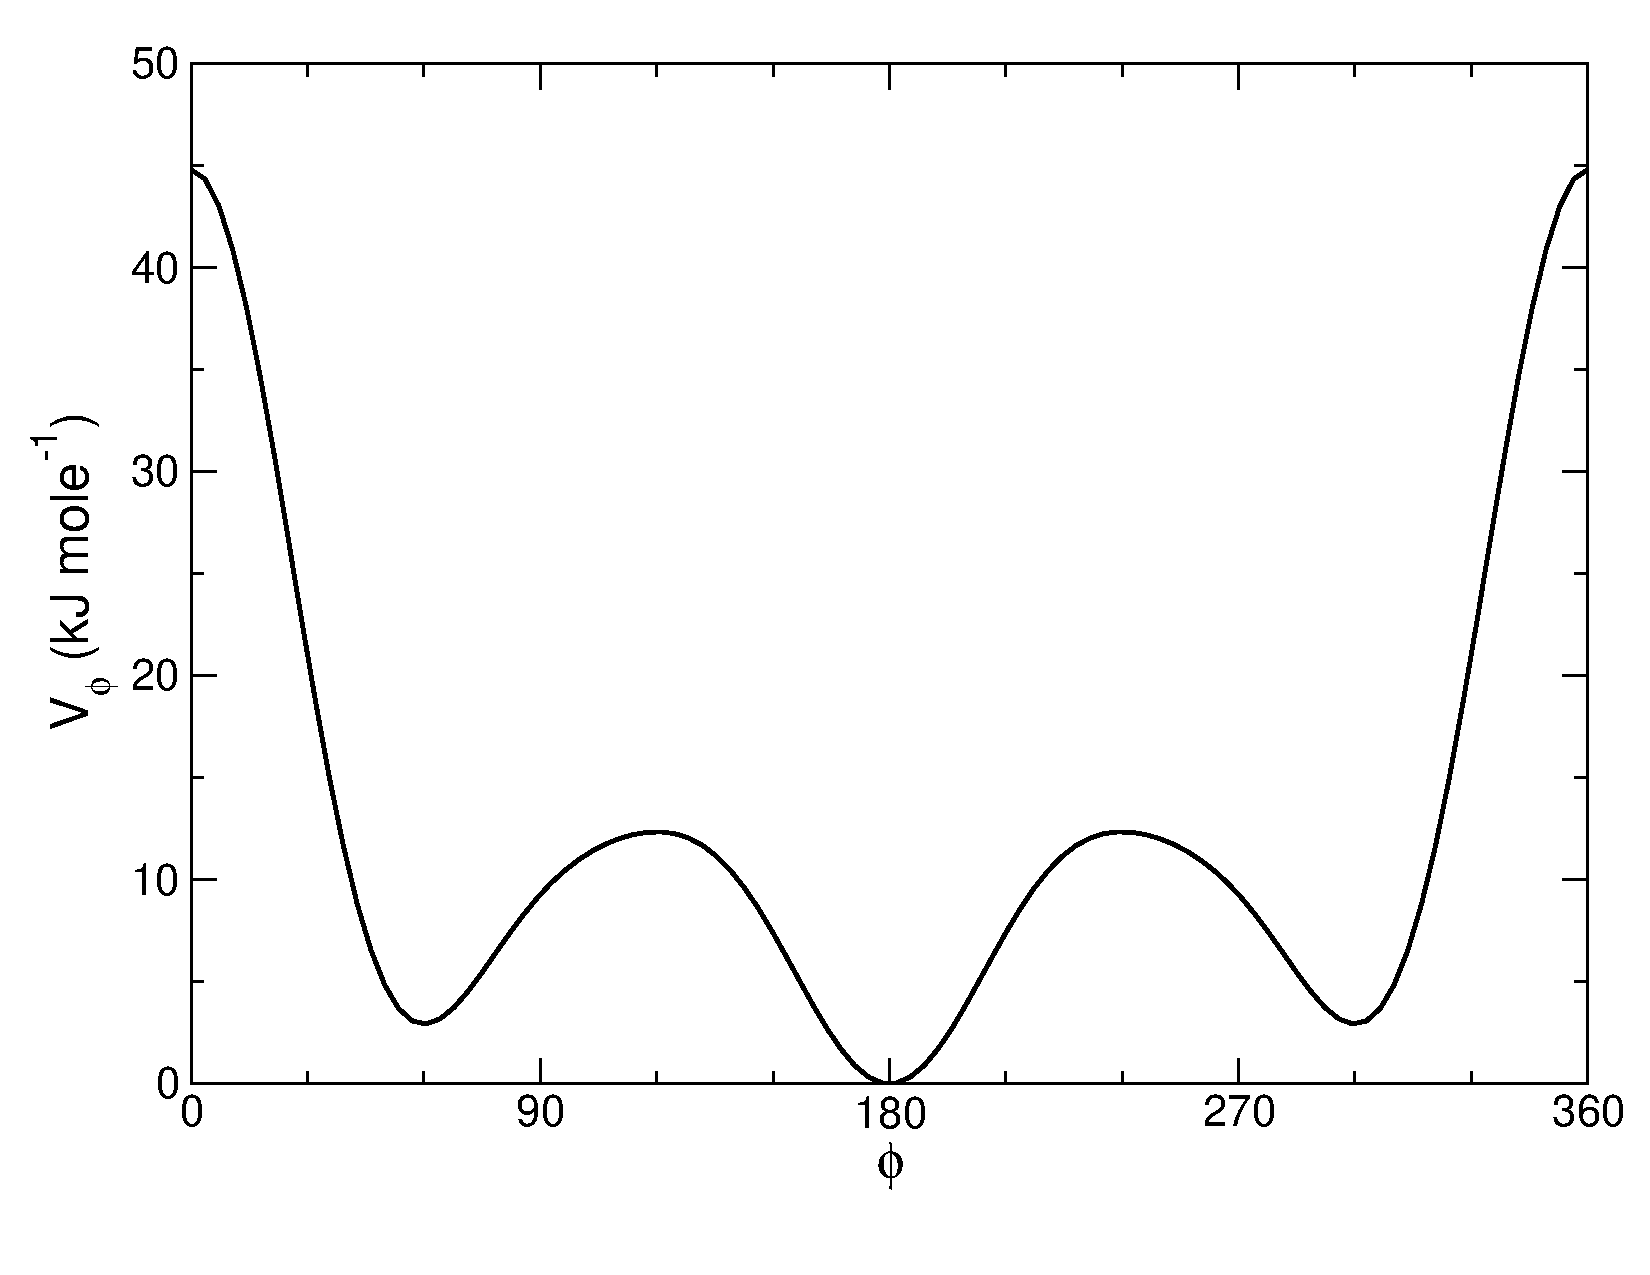
\includegraphics[width=8cm]{plots/f_rbs}}
\caption{Ryckaert-Bellemans dihedral potential.}
\label{fig:rbdih}
\end{figure}

({\bf Note:} The use of this potential implies exclusion of LJ interactions
between the first and the last atom of the dihedral, and $\psi$ is defined
according to the 'polymer convention' ($\psi_{trans}=0$).)

The RB dihedral function can also be used to include Fourier dihedrals
(see below):
\beq
V_{rb} (\phi_{ijkl}) ~=~ \frac{1}{2} \left[F_1(1+\cos(\phi)) + F_2(
1-\cos(2\phi)) + F_3(1+\cos(3\phi) + F_4(1-\cos(4\phi))\right]
\eeq
Because of the equalities \( \cos(2\phi) = 2\cos^2(\phi) - 1 \),
\( \cos(3\phi) = 4\cos^3(\phi) - 3\cos(\phi) \) and
\( \cos(4\phi) = 8\cos^4(\phi) - 8\cos^2(\phi) + 1 \)
one can translate the OPLS parameters to 
Ryckaert-Bellemans parameters as follows:
\beq
\displaystyle
\begin{array}{rcl}
\displaystyle C_0&=&F_2 + \frac{1}{2} (F_1 + F_3)\\
\displaystyle C_1&=&\frac{1}{2} (- F_1 + 3 \, F_3)\\
\displaystyle C_2&=& -F_2 + 4 \, F_4\\
\displaystyle C_3&=&-2 \, F_3\\
\displaystyle C_4&=&-4 \, F_4\\
\displaystyle C_5&=&0
\end{array}
\eeq 
with OPLS parameters in protein convention and RB parameters in
polymer convention (this yields a minus sign for the odd powers of 
cos$(\phi)$).\\
\noindent{\bf Note:} Mind the conversion from {\em kcal mol$^{-1}$} for 
literature OPLS and RB parameters to {\em kJ mol$^{-1}$} in {\gromacs}.\\
} % Brace matches ifthenelse test for gmxlite

\subsubsection{Proper dihedrals: Fourier function}
The OPLS potential function is given as the first three
or four~\cite{Jorgensen2005a} cosine terms of a Fourier series.
In {\gromacs} the four term function is implemented:
\beq
V_{F} (\phi_{ijkl}) ~=~ \frac{1}{2} \left[C_1(1+\cos(\phi)) + C_2(
1-\cos(2\phi)) + C_3(1+\cos(3\phi) + C_4(1+\cos(4\phi))\right],
\eeq
\ifthenelse{\equal{\gmxlite}{1}}{}{Internally {\gromacs}
uses the Ryckaert-Bellemans code
to compute Fourier dihedrals (see above), because this is more efficient.}\\
\noindent{\bf Note:} Mind the conversion from {\em kcal mol$^{-1}$} for 
literature OPLS parameters to {\em kJ mol$^{-1}$} in {\gromacs}.\\

\ifthenelse{\equal{\gmxlite}{1}}{}{
\subsection{\normindex{Tabulated interaction function}s}
For full flexibility, any functional shape can be used for
bonds, angles and dihedrals through user supplied tabulated functions.
The functional shapes are:
\bea
V_b(r_{ij})      &=& k \, f^b_n(r_{ij}) \\
V_a(\tijk)       &=& k \, f^a_n(\tijk) \\
V_d(\phi_{ijkl}) &=& k \, f^d_n(\phi_{ijkl})
\eea
where $k$ is a force constant in units of energy
and $f$ is a cubic spline function, for details see \ssecref{cubicspline}.
For each interaction the force constant $k$ and the table number $n$
are specified in the topology.
The are two different types of bonds, one that generates exclusions
and one that does not.
For details see \tabref{topfile2}.
The table files are supplied to the {\tt mdrun} program.
After the table file name an underscore, the letter 'b' for bonds,
'a' for angles or 'd' for dihedrals and the table number are appended.
For example, for a bond with $n=0$ (and using the default table file name)
the table is read from the file {\tt table\_b0.xvg}.
The format for the table files is three columns with $x$, $f(x)$, $-f'(x)$,
where $x$ should be uniformly spaced.
The setup of the tables is as follows:
\\{\bf bonds}:
$x$ is the distance in nanometers, for distances beyond the table length
cause {\tt mdrun} to quit with an error message
\\{\bf angles}:
$x$ is the angle in degrees, the table should go from
0 up to and including 180 degrees, the derivative is taken in degrees
\\{\bf dihedrals}:
$x$ is the dihedral angle in degrees, the table should go from
-180 up to and including 180 degrees,
the IUPAC/IUB convention is used, i.e. zero is cis,
the derivative is taken in degrees
} % Brace matches ifthenelse test for gmxlite

\section{Restraints}
Special potentials are used for imposing restraints on the motion of
the system, either to avoid disastrous deviations, or to include
knowledge from experimental data. In either case they are not really
part of the force field and the reliability of the parameters is not
important. The potential forms, as implemented in {\gromacs}, are
mentioned just for the sake of completeness.

\subsection{\swapindex{Position}{restraint}s}
\label{sec:posre}
These are used to restrain particles to fixed reference positions
$\ve{R}_i$. They can be used during equilibration in order to avoid
too drastic rearrangements of critical parts ({\eg} to restrain motion
in a protein that is subjected to large solvent forces when the
solvent is not yet equilibrated). Another application is the
restraining of particles in a shell around a region that is simulated
in detail, while the shell is only approximated because it lacks
proper interaction from missing particles outside the
shell. Restraining will then maintain the integrity of the inner
part. For spherical shells it is a wise procedure to make the force
constant depend on the radius, increasing from zero at the inner
boundary to a large value at the outer boundary. This feature has
not, however, been implemented in {\gromacs}.
\newcommand{\unitv}[1]{\hat{\bf #1}}
\newcommand{\halfje}[1]{\frac{#1}{2}}

The following form is used: 
\beq
V_{pr}(\ve{r}_i) = \halfje{1}k_{pr}|\rvi-\ve{R}_i|^2
\eeq
The potential is plotted in \figref{posres}.

\begin{figure}
\centerline{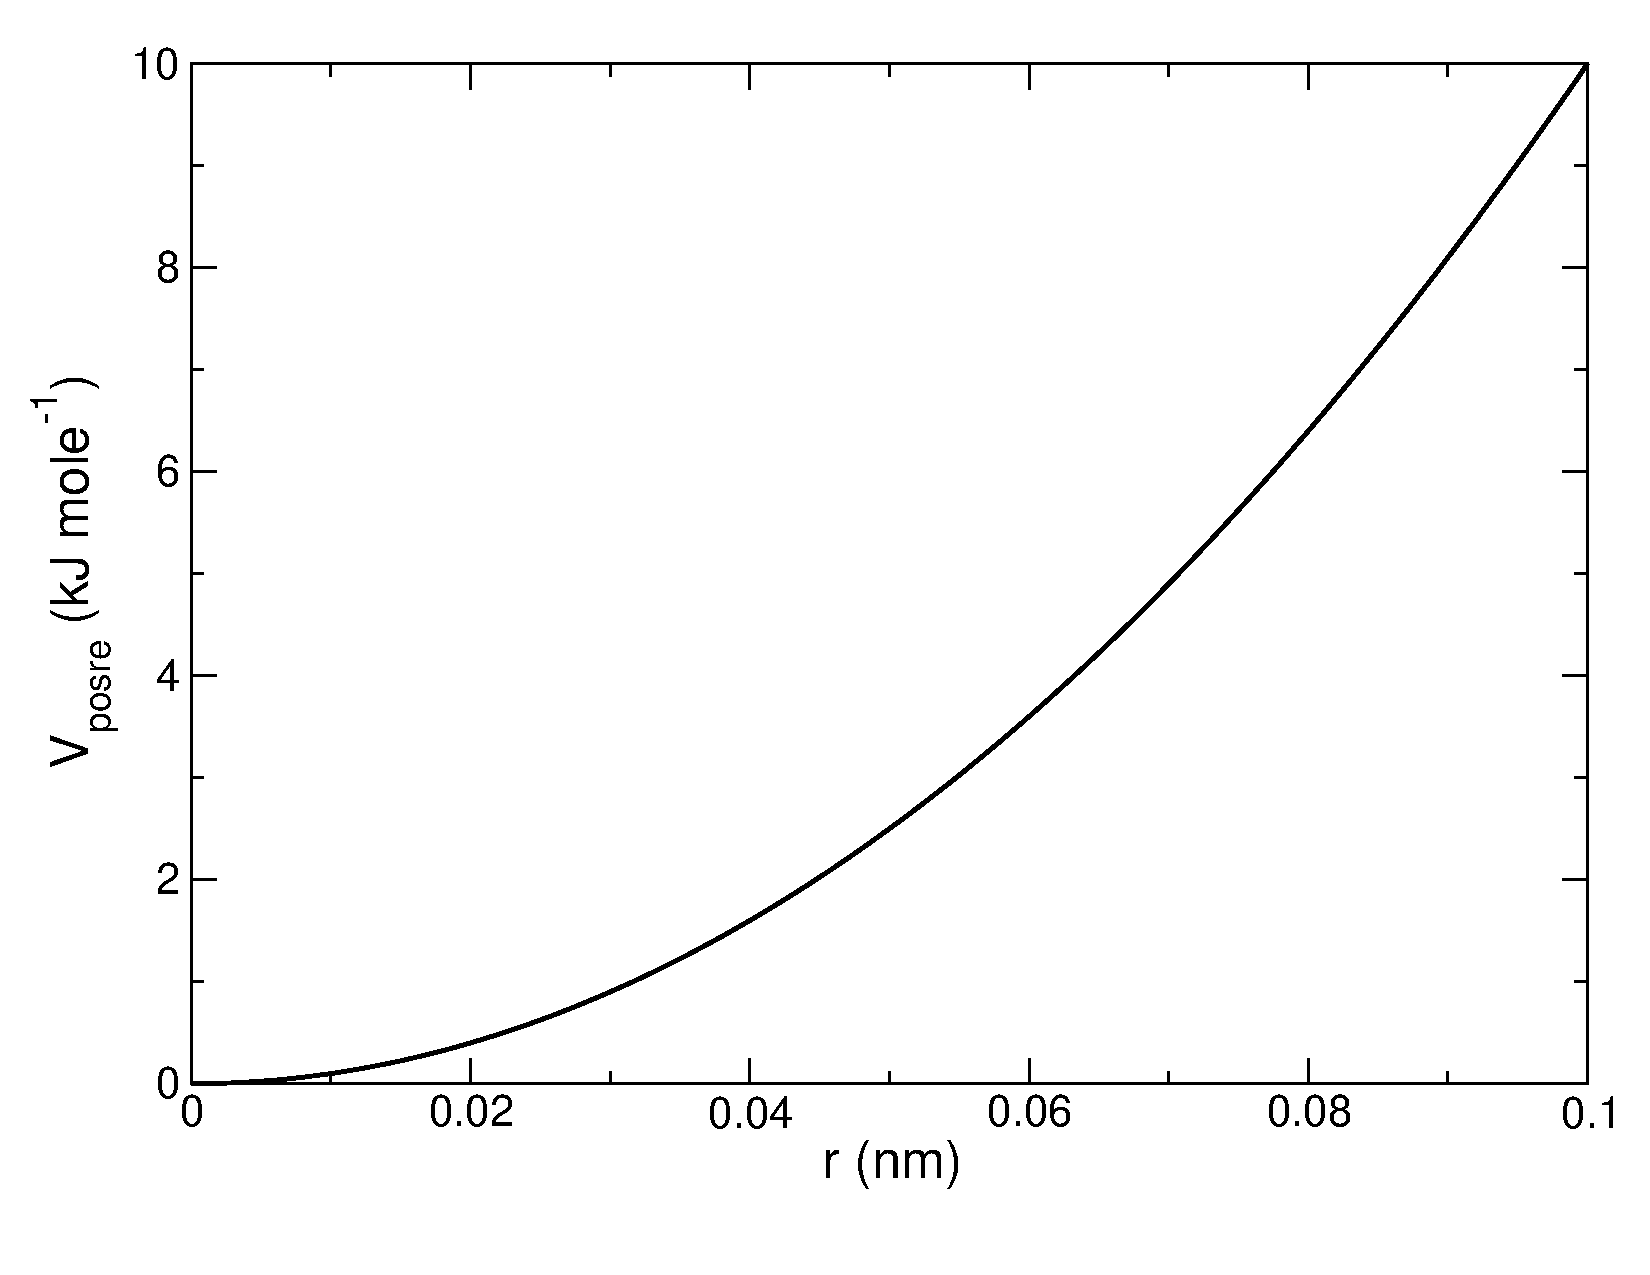
\includegraphics[width=8cm]{plots/f_pr}}
\caption{Position restraint potential.}
\label{fig:posres}
\end{figure}

The potential form can be rewritten without loss of generality as:
\beq
V_{pr}(\ve{r}_i) = \halfje{1} \left[ k_{pr}^x (x_i-X_i)^2 ~\unitv{x} + k_{pr}^y (y_i-Y_i)^2 ~\unitv{y} + k_{pr}^z (z_i-Z_i)^2 ~\unitv{z}\right]
\eeq

Now the forces are:
\beq
\begin{array}{rcl}
F_i^x &=& -k_{pr}^x~(x_i - X_i) \\
F_i^y &=& -k_{pr}^y~(y_i - Y_i) \\
F_i^z &=& -k_{pr}^z~(z_i - Z_i)
\end{array}
\eeq
Using three different force constants the position 
restraints can be turned on or off
in each spatial dimension; this means that atoms can be harmonically
restrained to a plane or a line.
Position restraints are applied to a special fixed list of atoms. Such a
list is usually generated by the \normindex{pdb2gmx} program.

\ifthenelse{\equal{\gmxlite}{1}}{}{
\subsection{\swapindex{Angle}{restraint}s}
\label{sec:angres}
These are used to restrain the angle between two pairs of particles
or between one pair of particles and the Z-axis.
The functional form is similar to that of a proper dihedral.
For two pairs of atoms: 
\beq
V_{ar}(\ve{r}_i,\ve{r}_j,\ve{r}_k,\ve{r}_l)
        = k_{ar}(1 - \cos(n (\theta - \theta_0))
        )
,~~~~\mbox{where}~~
\theta = \arccos\left(\frac{\ve{r}_j -\ve{r}_i}{\|\ve{r}_j -\ve{r}_i\|}
 \cdot \frac{\ve{r}_l -\ve{r}_k}{\|\ve{r}_l -\ve{r}_k\|} \right)
\eeq
For one pair of atoms and the Z-axis: 
\beq
V_{ar}(\ve{r}_i,\ve{r}_j) = k_{ar}(1 - \cos(n (\theta - \theta_0))
        )
,~~~~\mbox{where}~~
\theta = \arccos\left(\frac{\ve{r}_j -\ve{r}_i}{\|\ve{r}_j -\ve{r}_i\|}
 \cdot \left( \begin{array}{c} 0 \\ 0 \\ 1 \\ \end{array} \right) \right)
\eeq
A multiplicity ($n$) of 2 is useful when you do not want to distinguish
between parallel and anti-parallel vectors.
The equilibrium angle $\theta$ should be between 0 and 180 degrees
for multiplicity 1 and between 0 and 90 degrees for multiplicity 2.


\subsection{\swapindex{Dihedral}{restraint}s}
\label{sec:dihres}
These are used to restrain the dihedral angle $\phi$ defined by four particles
as in an improper dihedral (sec.~\ref{sec:imp}) but with a slightly
modified potential. Using
\beq
\phi' = \left(\phi-\phi_0\right) ~{\rm MOD}~ 2\pi
\eeq
where $\phi_0$ is the reference angle, the potential is defined as:
\beq
V_{dihr}(\phi') ~=~ \left\{
\begin{array}{lcllll}
\half k_{dihr}(\phi'-\phi_0-\Delta\phi)^2      
                &\mbox{for}&     \phi' & >   & \Delta\phi       \\[1.5ex]
0               &\mbox{for}&     \phi' & \le & \Delta\phi       \\[1.5ex]
\end{array}\right.
\label{eqn:dihre}
\eeq
where $\Delta\phi$ is a user defined angle and $k_{dihr}$ is the force 
constant.
{\bf Note} that in the input in topology files, angles are given in degrees and
force constants in kJ/mol/rad$^2$.
} % Brace matches ifthenelse test for gmxlite

\subsection{\swapindex{Distance}{restraint}s}
\label{sec:disre}
Distance restraints 
add a penalty to the potential when the distance between specified
pairs of atoms exceeds a threshold value. They are normally used to
impose experimental restraints, as from for instance experiments in nuclear
magnetic resonance (NMR), on the motion of the system. Thus MD can be
used for structure refinement using NMR data\index{nmr
refinement}\index{refinement,nmr}.
In {\gromacs} there are three ways to impose restraints on pairs of atoms:
\begin{itemize}
\item Simple harmonic restraints: use {\tt [ bonds ]} type 6
\ifthenelse{\equal{\gmxlite}{1}}
{.}
{(see \secref{excl}).}
\item Piecewise linear/harmonic restraints: {\tt [ bonds ]} type 10.
\item Complex NMR distance restraints, optionally with pair, time and/or
ensemble averaging.
\end{itemize}
The last two options will be detailed now.

The potential form for distance restraints is quadratic below a specified
lower bound and between two specified upper bounds and linear beyond the
largest bound (see \figref{dist}).
\beq
V_{dr}(r_{ij}) ~=~ \left\{
\begin{array}{lcllllll}
\half k_{dr}(r_{ij}-r_0)^2      
                &\mbox{for}&     &     & r_{ij} & < & r_0       \\[1.5ex]
0               &\mbox{for}& r_0 & \le & r_{ij} & < & r_1       \\[1.5ex]
\half k_{dr}(r_{ij}-r_1)^2      
                &\mbox{for}& r_1 & \le & r_{ij} & < & r_2       \\[1.5ex]
\half k_{dr}(r_2-r_1)(2r_{ij}-r_2-r_1)  
                &\mbox{for}& r_2 & \le & r_{ij} &   &
\end{array}\right.
\label{eqn:disre}
\eeq

\begin{figure}
\centerline{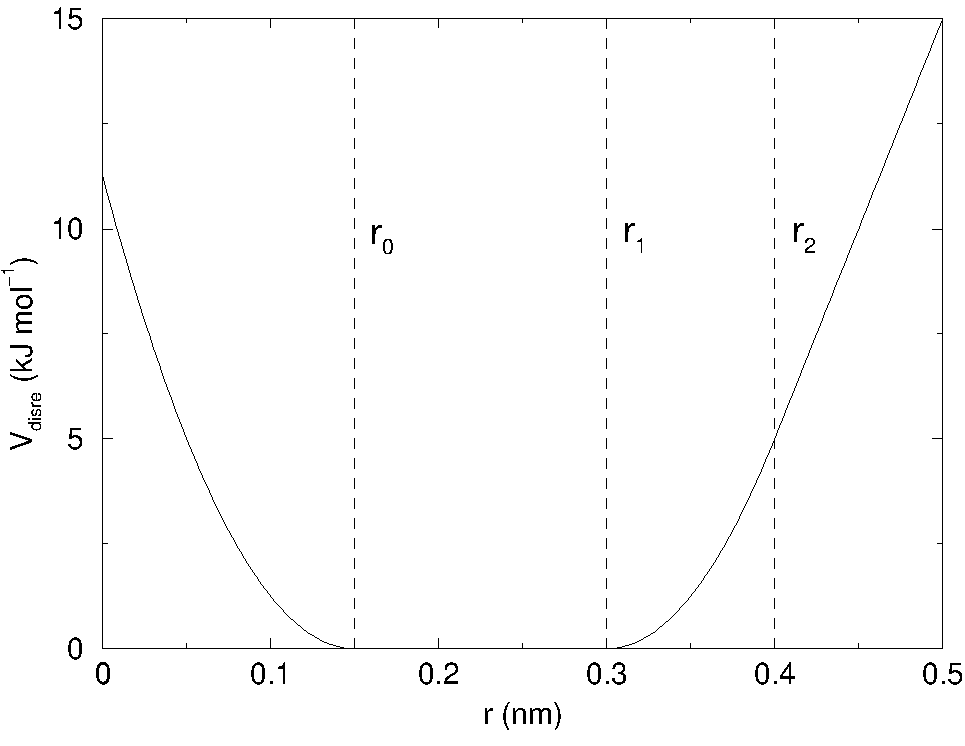
\includegraphics[width=8cm]{plots/f_dr}}
\caption{Distance Restraint potential.}
\label{fig:dist}
\end{figure}

The forces are
\beq
\ve{F}_i~=~ \left\{
\begin{array}{lcllllll}
-k_{dr}(r_{ij}-r_0)\frac{\rvij}{r_{ij}} 
                &\mbox{for}&     &     & r_{ij} & < & r_0       \\[1.5ex]
0               &\mbox{for}& r_0 & \le & r_{ij} & < & r_1       \\[1.5ex]
-k_{dr}(r_{ij}-r_1)\frac{\rvij}{r_{ij}} 
                &\mbox{for}& r_1 & \le & r_{ij} & < & r_2       \\[1.5ex]
-k_{dr}(r_2-r_1)\frac{\rvij}{r_{ij}}    
                &\mbox{for}& r_2 & \le & r_{ij} &   &
\end{array} \right.
\eeq

For restraints not derived from NMR data, this functionality
will usually suffice and a section of {\tt [ bonds ]} type 10
can be used to apply individual restraints between pairs of atoms,
\ifthenelse{\equal{\gmxlite}{1}}
{atoms.}
{atoms, see \ssecref{topfile}.}
For applying restraints derived from NMR measurements more complex
functionality might be required, which is provided through
the {\tt [ distance\_restraints ]} section and is described below.

\ifthenelse{\equal{\gmxlite}{1}}{}{
\subsubsection{Time averaging}
Distance restraints based on instantaneous distances can potentially reduce
the fluctuations in a molecule significantly. This problem can be overcome by restraining
to a {\em time averaged} distance~\cite{Torda89}.
The forces with time averaging are:
\beq
\ve{F}_i~=~ \left\{
\begin{array}{lcllllll}
-k^a_{dr}(\bar{r}_{ij}-r_0)\frac{\rvij}{r_{ij}}   
                &\mbox{for}&     &     & \bar{r}_{ij} & < & r_0 \\[1.5ex]
0               &\mbox{for}& r_0 & \le & \bar{r}_{ij} & < & r_1 \\[1.5ex]
-k^a_{dr}(\bar{r}_{ij}-r_1)\frac{\rvij}{r_{ij}}   
                &\mbox{for}& r_1 & \le & \bar{r}_{ij} & < & r_2 \\[1.5ex]
-k^a_{dr}(r_2-r_1)\frac{\rvij}{r_{ij}}    
                &\mbox{for}& r_2 & \le & \bar{r}_{ij} &   &
\end{array} \right.
\eeq
where $\bar{r}_{ij}$ is given by an exponential running average with decay time $\tau$:
\beq
\bar{r}_{ij} ~=~ < r_{ij}^{-3} >^{-1/3}
\label{eqn:rav}
\eeq
and the force constant $k^a_{dr}$ is switched on slowly to compensate for
the lack of history at the beginning of the simulation:
\beq
k^a_{dr} = k_{dr} \left(1-\exp\left(-\frac{t}{\tau}\right)\right)
\eeq
Because of the time averaging we can no longer speak of a distance restraint
potential.

This way an atom can satisfy two incompatible distance restraints 
{\em on average} by moving between two positions. 
An example would be an amino-acid side-chain which is rotating around
its $\chi$ dihedral angle, thereby coming close to various other groups.
Such a mobile side chain can give rise to multiple NOEs that can not be
fulfilled by a single structure.

The computation of the time
averaged distance in the {\tt mdrun} program is done in the following fashion:
\beq
\begin{array}{rcl}
\overline{r^{-3}}_{ij}(0)       &=& r_{ij}(0)^{-3}      \\
\overline{r^{-3}}_{ij}(t)       &=& \overline{r^{-3}}_{ij}(t-\Delta t)~\exp{\left(-\frac{\Delta t}{\tau}\right)} + r_{ij}(t)^{-3}\left[1-\exp{\left(-\frac{\Delta t}{\tau}\right)}\right]
\label{eqn:ravdisre}
\end{array}
\eeq

When a pair is within the bounds it can still feel a force,
because the time averaged distance can still be beyond a bound.
To prevent the protons from being pulled too close together a mixed
approach can be used. In this approach the penalty is zero when the
instantaneous distance is within the bounds, otherwise the violation is
the square root of the product of the instantaneous violation and the 
time averaged violation:
\beq
\ve{F}_i~=~ \left\{
\begin{array}{lclll}
k^a_{dr}\sqrt{(r_{ij}-r_0)(\bar{r}_{ij}-r_0)}\frac{\rvij}{r_{ij}}   
    & \mbox{for} & r_{ij} < r_0 & \mbox{and} & \bar{r}_{ij} < r_0 \\[1.5ex]
-k^a _{dr} \,
  \mbox{min}\left(\sqrt{(r_{ij}-r_1)(\bar{r}_{ij}-r_1)},r_2-r_1\right)
  \frac{\rvij}{r_{ij}}   
    & \mbox{for} & r_{ij} > r_1 & \mbox{and} & \bar{r}_{ij} > r_1 \\[1.5ex]
0               &\mbox{else}
\end{array} \right.
\eeq

\subsubsection{Averaging over multiple pairs} 

Sometimes it is unclear from experimental data which atom pair
gives rise to a single NOE, in other occasions it can be obvious that
more than one pair contributes due to the symmetry of the system, {\eg} a
methyl group with three protons. For such a group it is not possible 
to distinguish between the protons, therefore they should all be taken into
account when calculating the distance between this methyl group and another
proton (or group of protons).
Due to the physical nature of magnetic resonance, the intensity of the
NOE signal is inversely proportional to the sixth power of the inter-atomic 
distance.
Thus, when combining atom pairs, 
a fixed list of $N$ restraints may be taken together, 
where the apparent ``distance'' is given by:
\beq
r_N(t) = \left [\sum_{n=1}^{N} \bar{r}_{n}(t)^{-6} \right]^{-1/6}
\label{eqn:rsix}
\eeq
where we use $r_{ij}$ or \eqnref{rav} for the $\bar{r}_{n}$.
The $r_N$ of the instantaneous and time-averaged distances
can be combined to do a mixed restraining as indicated above.
As more pairs of protons contribute to the same NOE signal, the intensity
will increase, and the summed ``distance'' will be shorter than any of
its components due to the reciprocal summation. 

There are two options for distributing the forces over the atom pairs.
In the conservative option the force is defined as the derivative of the
restraint potential with respect to the coordinates. This results in
a conservative potential when time averaging is not used.
The force distribution over the pairs is proportional to $r^{-6}$.
This means that a close pair feels a much larger force than a distant pair,
which might lead to a 'too rigid' molecule.
The other option is an equal force distribution. In this case each pair
feels $1/N$ of the derivative of the restraint potential with respect to 
$r_N$. The advantage of this method is that more conformations might be
sampled, but the non-conservative nature of the forces can lead to
local heating of the protons.

It is also possible to use {\em ensemble averaging} using multiple
(protein)  molecules. In this case the bounds should be lowered as in:
\beq
\begin{array}{rcl}
r_1     &~=~&   r_1 * M^{-1/6}  \\
r_2     &~=~&   r_2 * M^{-1/6}
\end{array}
\eeq
where $M$ is the number of molecules. The {\gromacs} preprocessor {\tt grompp}
can do this automatically when the appropriate option is given.
The resulting ``distance'' is 
then used to calculate the scalar force according to:
\beq
\begin{array}{rcl}
\ve{F}_i~=~&~0 \hspace{4cm}  & r_{N} < r_1         \\
  = ~&-~ k_{dr}(r_{N}-r_1)\frac{\rvij}{r_{ij}} & r_1 \le r_{N} < r_2 \\
  = ~&-~ k_{dr}(r_2-r_1)\frac{\rvij}{r_{ij}}    & r_{N} \ge r_2 
\end{array}
\eeq
where $i$ and $j$ denote the atoms of all the 
pairs that contribute to the NOE signal.

\subsubsection{Using distance restraints}

A list of distance restrains based on NOE data can be added to a molecule
definition in your topology file, like in the following example:

\begin{tabular}{ccccccccc}
\multicolumn{9}{l}{[ distance\_restraints ]}\\
; ai & aj  &  type & index & type' &  low &   up1 &    up2  &  fac\\
10  &   16  &    1  &     0  &     1  &    0.0  &   0.3  &   0.4  &   1.0\\
10  &   28  &    1  &     1  &     1  &    0.0  &   0.3  &   0.4  &   1.0\\
10  &   46  &    1  &     1  &     1  &    0.0  &   0.3  &   0.4  &   1.0\\
16  &   22  &    1  &     2  &     1  &    0.0  &   0.3  &   0.4  &   2.5\\
16  &   34  &    1  &     3  &     1  &    0.0  &   0.5  &   0.6  &   1.0\\
\end{tabular}


In this example a number of features can be found.  In columns {\tt
ai} and {\tt aj} you find the atom numbers of the particles to be
restrained. The {\tt type} column should always be 1.  As explained in
~\secref{disre}, multiple distances can contribute to a single NOE
signal. In the topology this can be set using the {\tt index}
column. In our example, the restraints 10-28 and 10-46 both have index
1, therefore they are treated simultaneously.  An extra requirement
for treating restraints together, is that the restraints should be on
successive lines, without any other intervening restraint.  The {\tt
type'} column will usually be 1, but can be set to 2 to obtain a
distance restraint which will never be time and ensemble averaged;
this can be useful for restraining hydrogen bonds.  The columns {\tt
low}, {\tt up1} and {\tt up2} hold the values of $r_0$, $r_1$ and
$r_2$ from ~\eqnref{disre}.  In some cases it can be useful to have
different force constants for some restraints; this is controlled by
the column {\tt fac}.  The force constant in the parameter file is
multiplied by the value in the column {\tt fac} for each restraint.

Some parameters for NMR refinement can be specified in the
{\tt grompp.mdp} file:
\begin{description}
\item[{\tt disre}: type of distance restraining.]
        The {\tt disre} variable sets the type of distance restraint.
        {\tt no/simple} turns the distance restraints off/on.
        When multiple proteins or peptides are present in one 
        simulation box, ensemble averaging 
        can be turned on by setting {\tt disre = ensemble}.
	Normally one would perform ensemble averaging over multiple
	subsystems, each in a separate box, using {\tt mdrun -multi};
	supply {\tt topol0.tpr}, {\tt topol1.tpr}, ... with different
	coordinates and/or velocities.
\item[{\tt disre\_weighting}: force-weighting in restraints with
         multiple pairs.]
        By default, the force due to the distance restraint is distributed equally
        over all the pairs involved in the restraint. This can also be
        explicitly selected with
        {\tt disre\_weighting = equal}. 
        If you instead set this option to {\tt disre\_weighting = conservative}
        you get conservative forces when {\tt disre\_tau = 0}.
\item[{\tt disre\_mixed}: how to calculate the violations.]
        {\tt disre\_mixed = no} gives normal time-averaged violations.
        When {\tt disre\_mixed = yes} the square root of the
        product of the time-averaged and the instantaneous
        violations is used.
\item[{\tt disre\_fc}: force constant $k_{dr}$ for distance restraints.] 
        $k_{dr}$  (\eqnref{disre}) can be set
        as variable {\tt disre\_fc = 1000} for a force constant of
        1000 {kJ mol$^{-1}$ nm$^{-2}$}. This value is multiplied by
        the value in the {\tt fac} column in the distance restraint
        entries in the topology file.
\item[{\tt disre\_tau}: time constant for restraints.] 
        $\tau$ (\eqnref{ravdisre}) can be set
        as variable {\tt disre\_tau = 10} for a time constant of
        10 ps. Time averaging can be turned off by setting {\tt disre\_tau}
        to 0.
\item[{\tt nstdisreout}: pair distance output frequency.]
        Determines how often the time-averaged and 
        instantaneous distances of all atom pairs involved in
        distance restraints are written to the energy file.
\end{description}
} % Brace matches ifthenelse test for gmxlite

\newcommand{\SSS}{{\mathbf S}}
\newcommand{\DD}{{\mathbf D}}
\newcommand{\RR}{{\mathbf R}}

\ifthenelse{\equal{\gmxlite}{1}}{}{
\subsection{\swapindex{Orientation}{restraint}s}
\label{sec:orire}
This section describes how orientations between vectors,
as measured in certain NMR experiments, can be calculated
and restrained in MD simulations.
The presented refinement methodology and a comparison of results
with and without time and ensemble averaging have been
published~\cite{Hess2003}.
\subsubsection{Theory}
In an NMR experiment orientations of vectors can be measured when a 
molecule does not tumble completely isotropically in the solvent.
Two examples of such orientation measurements are
residual \normindex{dipolar couplings}
(between two nuclei) or chemical shift anisotropies.
An observable for a vector $\ve{r}_i$ can be written as follows:
\beq
\delta_i = \frac{2}{3} \mbox{tr}(\SSS\DD_i)
\eeq
where $\SSS$ is the dimensionless order tensor of the molecule.
The tensor $\DD_i$ is given by:
\beq
\label{orient_def}
\DD_i = \frac{c_i}{\|\ve{r}_i\|^\alpha} \left(
%\begin{array}{lll}
%3 r_x r_x - \ve{r}\cdot\ve{r} & 3 r_x r_y & 3 r_x r_z \\
%3 r_x r_y                     & 3 r_y r_y - \ve{r}\cdot\ve{r} & 3yz \\
%3 r_x r_z                     & 3 r_y r_z & 3 r_z r_z - \ve{r}\cdot\ve{r}
%\end{array} \right)
\begin{array}{lll}
3 x x - 1 & 3 x y     & 3 x z     \\
3 x y     & 3 y y - 1 & 3 y z     \\
3 x z     & 3 y z     & 3 z z - 1 \\
\end{array} \right)
\eeq
\beq
\mbox{with:} \quad 
x=\frac{r_{i,x}}{\|\ve{r}_i\|}, \quad
y=\frac{r_{i,y}}{\|\ve{r}_i\|}, \quad 
z=\frac{r_{i,z}}{\|\ve{r}_i\|}
\eeq
For a dipolar coupling $\ve{r}_i$ is the vector connecting the two
nuclei, $\alpha=3$ and the constant $c_i$ is given by:
\beq
c_i = \frac{\mu_0}{4\pi} \gamma_1^i \gamma_2^i \frac{\hbar}{4\pi}
\eeq
where $\gamma_1^i$ and $\gamma_2^i$ are the gyromagnetic ratios of the
two nuclei.

The order tensor is symmetric and has trace zero. Using a rotation matrix
${\mathbf T}$ it can be transformed into the following form:
\beq
{\mathbf T}^T \SSS {\mathbf T} = s \left( \begin{array}{ccc}
-\frac{1}{2}(1-\eta) & 0                    & 0 \\
0                    & -\frac{1}{2}(1+\eta) & 0 \\
0                    & 0                    & 1
\end{array} \right)
\eeq
where $-1 \leq s \leq 1$ and $0 \leq \eta \leq 1$.
$s$ is called the order parameter and $\eta$ the asymmetry of the
order tensor $\SSS$. When the molecule tumbles isotropically in the
solvent, $s$ is zero, and no orientational effects can be observed
because all $\delta_i$ are zero.

%\newpage

\subsubsection{Calculating orientations in a simulation}
For reasons which are explained below, the $\DD$ matrices are calculated
which respect to a reference orientation of the molecule. The orientation
is defined by a rotation matrix $\RR$ which is needed to least-squares fit
the current coordinates of a selected set of atoms onto
a reference conformation. The reference conformation is the starting
conformation of the simulation. In case of ensemble averaging, which will
be treated later, the structure is taken from the first subsystem.
The calculated $\DD_i^c$ matrix is given by:
\begin{equation}
\label{D_rot}
\DD_i^c(t) = \RR(t) \DD_i(t) \RR^T(t)
\end{equation}
The calculated orientation for vector $i$ is given by:
\beq
\delta^c_i(t) = \frac{2}{3} \mbox{tr}(\SSS(t)\DD_i^c(t))
\eeq
The order tensor $\SSS(t)$ is usually unknown.
A reasonable choice for the order tensor is the tensor
which minimizes the (weighted) mean square difference between the calculated
and the observed orientations:
\begin{equation}
\label{S_msd}
MSD(t) = \left(\sum_{i=1}^N w_i\right)^{-1} \sum_{i=1}^N w_i (\delta_i^c (t) -\delta_i^{exp})^2
\end{equation}
To properly combine different types of measurements the unit of $w_i$ should
be such that all terms are dimensionless. This means the unit of $w_i$
is the unit of $\delta_i$ to the power $-2$.
Note that scaling all $w_i$ with a constant factor does not influence
the order tensor.

\subsubsection{Time averaging}
Since the tensors $\DD_i$ fluctuate rapidly in time, much faster than can
be observed in experiment, they should be time averaged in the simulation.
However, in a simulation the time as well as the number of copies of
a molecule is limited. Usually one can not obtain a converged average
of the $\DD_i$ tensors over all orientations of the molecule.
If one assumes that the average orientations of the $\ve{r}_i$ vectors
within the molecule converge much faster than the tumbling time of
the molecule, the tensor can be averaged in an axis system which
rotates with the molecule, as expressed by equation~(\ref{D_rot}).
The time averaged tensors are calculated
using an exponentially decaying memory function:
\beq
\DD^a_i(t) = \frac{\displaystyle
\int_{u=t_0}^t \DD^c_i(u) \exp\left(-\frac{t-u}{\tau}\right)\mbox{d} u
}{\displaystyle
\int_{u=t_0}^t \exp\left(-\frac{t-u}{\tau}\right)\mbox{d} u
}
\eeq
Assuming that the order tensor $\SSS$ fluctuates slower than the
$\DD_i$, the time averaged orientation can be calculated as:
\beq
\delta_i^a(t) = \frac{2}{3} \mbox{tr}(\SSS(t) \DD_i^a(t))
\eeq
where the order tensor $\SSS(t)$ is calculated using expression~(\ref{S_msd})
with $\delta_i^c(t)$ replaced by $\delta_i^a(t)$.

\subsubsection{Restraining}
The simulated structure can be restrained by applying a force proportional
to the difference between the calculated and the experimental orientations.
When no time averaging is applied a proper potential can be defined as:
\beq
V = \frac{1}{2} k \sum_{i=1}^N w_i (\delta_i^c (t) -\delta_i^{exp})^2
\eeq
where the unit of $k$ is the unit of energy.
Thus the effective force constant for restraint $i$ is $k w_i$.
The forces are given by minus the gradient of $V$.
The force $\ve{F}\!_i$ working on vector $\ve{r}_i$ is:
\begin{eqnarray*}
\ve{F}\!_i(t) 
& = & - \frac{\mbox{d} V}{\mbox{d}\ve{r}_i} \\
& = & -k w_i (\delta_i^c (t) -\delta_i^{exp}) \frac{\mbox{d} \delta_i (t)}{\mbox{d}\ve{r}_i} \\
& = & -k w_i (\delta_i^c (t) -\delta_i^{exp})
\frac{2 c_i}{\|\ve{r}\|^{2+\alpha}} \left(2 \RR^T \SSS \RR \ve{r}_i - \frac{2+\alpha}{\|\ve{r}\|^2} \mbox{tr}(\RR^T \SSS \RR \ve{r}_i \ve{r}_i^T) \ve{r}_i \right)
\end{eqnarray*}

\subsubsection{Ensemble averaging}
Ensemble averaging can be applied by simulating a system of $M$ subsystems
which each contain an identical set of orientation restraints. The systems only
interact via the orientation restraint potential which is defined as:
\beq
V = M \frac{1}{2} k \sum_{i=1}^N w_i 
\langle \delta_i^c (t) -\delta_i^{exp} \rangle^2
\eeq
The force on vector $\ve{r}_{i,m}$ in subsystem $m$ is given by:
\beq
\ve{F}\!_{i,m}(t) = - \frac{\mbox{d} V}{\mbox{d}\ve{r}_{i,m}} =
-k w_i \langle \delta_i^c (t) -\delta_i^{exp} \rangle \frac{\mbox{d} \delta_{i,m}^c (t)}{\mbox{d}\ve{r}_{i,m}} \\
\eeq 

\subsubsection{Time averaging}
When using time averaging it is not possible to define a potential.
We can still define a quantity which gives a rough idea of the energy
stored in the restraints:
\beq
V = M \frac{1}{2} k^a \sum_{i=1}^N w_i 
\langle \delta_i^a (t) -\delta_i^{exp} \rangle^2
\eeq
The force constant $k_a$ is switched on slowly to compensate for the
lack of history at times close to $t_0$. It is exactly proportional
to the amount of average which has been accumulated:
\beq
k^a =
 k \, \frac{1}{\tau}\int_{u=t_0}^t \exp\left(-\frac{t-u}{\tau}\right)\mbox{d} u
\eeq
What really matters is the definition of the force. It is chosen to
be proportional to the square root of the product of the time averaged
and the instantaneous deviation.
Using only the time averaged deviation induces large oscillations.
The force is given by:
\beq
\ve{F}\!_{i,m}(t) =
%\left\{ \begin{array}{ll}
%0 & \mbox{for} \quad \langle \delta_i^a (t) -\delta_i^{exp} \rangle \langle \delta_i (t) -\delta_i^{exp} \rangle \leq 0 \\
%... & \mbox{for} \quad \langle \delta_i^a (t) -\delta_i^{exp} \rangle \langle \delta_i (t) -\delta_i^{exp} \rangle > 0 
%\end{array}
%\right.
\left\{ \begin{array}{ll}
0 & \quad \mbox{for} \quad a\, b \leq 0 \\
\displaystyle
k^a w_i \frac{a}{|a|} \sqrt{a\, b} \, \frac{\mbox{d} \delta_{i,m}^c (t)}{\mbox{d}\ve{r}_{i,m}}
& \quad \mbox{for} \quad a\, b > 0 
\end{array}
\right.
\eeq
\begin{eqnarray*}
a &=& \langle \delta_i^a (t) -\delta_i^{exp} \rangle \\
b &=& \langle \delta_i^c (t) -\delta_i^{exp} \rangle
\end{eqnarray*}

\subsubsection{Using orientation restraints}
Orientation restraints can be added to a molecule definition in
the topology in the section {\tt [ orientation\_restraints ]}.
Here we give an example section containing five N-H residual dipolar
coupling restraints:

\begin{tabular}{ccccccccc}
\multicolumn{9}{l}{[ orientation\_restraints ]}\\
; ai &  aj& type& exp.& label &alpha &  const. &   obs.&  weight \\
;    &    &     &     &       &      & Hz nm$^3$&      Hz & 1/Hz$^2$\\
  31 &  32  &   1  &   1  &    3  &    3  &   6.083  &  -6.73  &    1.0\\
  43 &  44  &   1  &   1  &    4  &    3  &   6.083  &  -7.87  &    1.0\\
  55 &  56  &   1  &   1  &    5  &    3  &   6.083  &  -7.13  &    1.0\\
  65 &  66  &   1  &   1  &    6  &    3  &   6.083  &  -2.57  &    1.0\\
  73 &  74  &   1  &   1  &    7  &    3  &   6.083  &  -2.10  &    1.0\\
\end{tabular}

The unit of the observable is Hz, but one can choose any other unit.
In columns {\tt
ai} and {\tt aj} you find the atom numbers of the particles to be
restrained. The {\tt type} column should always be 1.
The {\tt exp.} column denotes the experiment number, this starts
numbering at 1. For each experiment a separate order tensor $\SSS$
is optimized. The label should be a unique number larger than zero
for each restraint. The {\tt alpha} column contains the power $\alpha$ 
which is used in equation~(\ref{orient_def}) to calculate the orientation.
The {\tt const.} column contains the constant $c_i$ used in the same
equation. The constant should have the unit of the observable times
nm$^\alpha$. The column {\tt obs.} contains the observable, in any
unit you like. The last column contains the weights $w_i$, the unit
should be the inverse of the square of the unit of the observable.

Some parameters for orientation restraints can be specified in the
{\tt grompp.mdp} file, for a study of the effect of different
force constants and averaging times and ensemble averaging see~\cite{Hess2003}.
\begin{description}
\item[{\tt orire}: use orientation restraining.]
        {\tt no/yes} turns the distance restraints off/on.
	Ensemble averaging can be performed using {\tt mdrun -multi},
	which simulates multiple subsystems in separate boxes;
	supply {\tt topol0.tpr}, {\tt topol1.tpr}, ... with different
	coordinates and/or velocities.
\item[{\tt orire\_fc}: force constant $k$ for orientation restraints.] 
	The unit of $k$ is kJ mol$^{-1}$.
	Note that the force constant for a restraint is this force constant
	times the weight of the restraint.
	When set to zero one obtain the calculated orientation without
	affecting the simulation.
\item[{\tt orire\_tau}: time constant $\tau$ for restraints.] 
        Set {\tt orire\_tau = 10} for a time constant of
        10 ps. Time averaging can be turned off by setting {\tt orire\_tau}
        to 0.
\item[{\tt orire\_fitgrp}: the fit group for the restraints.]
	This group of atoms is used to determine the rotation $\RR$
	of the system with respect to the reference orientation.
	The reference orientation is the starting conformation of
	the first subsystem. For a protein {\tt backbone} should be
        a reasonable choice.	
\item[{\tt nstorireout}: orientation output frequency.]
        Determines how often the orientations for all restraints
        and the order tensor(s) $\SSS$ are written to the energy file.
	When using time and/or ensemble averaging, the time and ensemble
	averaged orientations as well as the instantaneous non-ensemble
	averaged orientations are written to the energy file.
	These can be analyzed using {\tt g\_energy}.
\end{description}
} % Brace matches ifthenelse test for gmxlite

\ifthenelse{\equal{\gmxlite}{1}}{}{
\section{Polarization}
Polarization can be treated by {\gromacs} by attaching
\normindex{shell} (\normindex{drude}) particles to atoms and/or
virtual sites. The energy of the shell particle is then minimized at
each time step in order to remain on the Born-Oppenheimer surface.

\subsection{Simple polarization}
This is merely a harmonic potential with equilibrium distance 0.

\subsection{Water polarization}
A special potential for water that allows anisotropic polarization of
a single shell particle~\cite{Maaren2001a}.

\subsection{Thole polarization}
Based on early work by \normindex{Thole}~\cite{Thole81} Roux and
coworkers have implemented potentials for molecules like
ethanol~\cite{Lamoureux2003a,Lamoureux2003b,Noskov2005a}. Within such
molecules there are intra-molecular interactions between shell
particles, however these must be screened because full Coulomb would
be too strong. The potential between two shell particles $i$ and $j$ is:
\newcommand{\rbij}{\bar{r}_{ij}}
\beq
V_{thole} ~=~ \frac{q_i q_j}{r_{ij}}\left[1-\left(1+\frac{\rbij}{2}\right){\rm exp}^{-\rbij}\right]
\eeq
(note that there is a sign error in Equation~1 of Noskov {\em et al.}~\cite{Noskov2005a}), where
\beq
\rbij ~=~ a\frac{r_{ij}}{(\alpha_i \alpha_j)^{1/6}}
\eeq
where a is a magic (dimensionless) constant, usually chosen to be
2.6~\cite{Noskov2005a} and $\alpha_i$, $\alpha_j$ are the polarizabilities
of the respective shell particles.

} % Brace matches ifthenelse test for gmxlite

\ifthenelse{\equal{\gmxlite}{1}}{}{
\section{Free energy interactions}
\label{sec:feia}
\index{free energy interactions}
\newcommand{\LAM}{\lambda}
\newcommand{\LL}{(1-\LAM)}
\newcommand{\dvdl}[1]{\frac{\partial #1}{\partial \LAM}}
This section describes the $\lambda$-dependence of the potentials
used for free energy calculations (see \secref{fecalc}).
All common types of potentials and constraints can be
interpolated smoothly from state A ($\lambda=0$) to state B
($\lambda=1$) and vice versa.
All bonded interactions are interpolated by linear interpolation
of the interaction parameters. Non-bonded interactions can be
interpolated linearly or via soft-core interactions.

\subsubsection{Harmonic potentials}
The example given here is for the bond potential, which is harmonic
in {\gromacs}. However,  these equations apply to the angle potential
and the improper dihedral potential as well.
\bea
V_b     &=&\half\left[\LL k_b^A + 
                \LAM k_b^B\right] \left[b - \LL b_0^A - \LAM b_0^B\right]^2  \\
\dvdl{V_b}&=&\half(k_b^B-k_b^A)
                \left[b - \LL b_0^A + \LAM b_0^B\right]^2 + 
		\nonumber\\
        & & \phantom{\half}(b_0^A-b_0^B) \left[b - \LL b_0^A -\LAM b_0^B\right]
		\left[\LL k_b^A + \LAM k_b^B \right]
\eea

\subsubsection{\gromosv{96} bonds and angles}
Fourth power bond stretching and cosine based angle potentials
are interpolated by linear interpolation of the force constant
and the equilibrium position. Formulas are not given here.

\subsubsection{Proper dihedrals}
For the proper dihedrals, the equations are somewhat more complicated:
\bea
V_d     &=&\left[\LL k_d^A + \LAM k_d^B \right]
        \left( 1+ \cos\left[n_{\phi} \phi - 
		    \LL \phi_s^A - \LAM \phi_s^B
		    \right]\right)\\
\dvdl{V_d}&=&(k_d^B-k_d^A) 
         \left( 1+ \cos
		 \left[
		    n_{\phi} \phi- \LL \phi_s^A - \LAM \phi_s^B
		 \right]
	 \right) +
	 \nonumber\\
        &&(\phi_s^B - \phi_s^A) \left[\LL k_d^A - \LAM k_d^B\right] 
        \sin\left[  n_{\phi}\phi - \LL \phi_s^A - \LAM \phi_s^B \right]
\eea
{\bf Note:} that the multiplicity $n_{\phi}$ can not be parameterized
because the function should remain periodic on the interval $[0,2\pi]$.

\subsubsection{Tabulated bonded interactions}
For tabulated bonded interactions only the force constant can interpolated:
\bea
      V  &=& (\LL k^A + \LAM k^B) \, f \\
\dvdl{V} &=& (k^B - k^A) \, f
\eea

\subsubsection{Coulomb interaction}
The \normindex{Coulomb} interaction between two particles 
of which the charge varies with $\LAM$ is:
\bea
V_c &=& \frac{f}{\epsrf \rij}\left[\LL q_i^A q_j^A + \LAM\, q_i^B q_j^B\right] \\
\dvdl{V_c}&=& \frac{f}{\epsrf \rij}\left[- q_i^A q_j^A + q_i^B q_j^B\right]
\eea
where $f = \frac{1}{4\pi \varepsilon_0} = 138.935\,485$ (see \chref{defunits})

\subsubsection{Coulomb interaction with \normindex{reaction field}}
The coulomb interaction including a reaction field, between two particles 
of which the charge varies with $\LAM$ is:
\bea
V_c     &=& f\left[\frac{1}{\rij} + k_{rf}~ \rij^2 -c_{rf}\right]
             \left[\LL q_i^A q_j^A + \LAM\, q_i^B q_j^B\right] \\
\dvdl{V_c}&=& f\left[\frac{1}{\rij} + k_{rf}~ \rij^2 -c_{rf}\right]
               \left[- q_i^A q_j^A + q_i^B q_j^B\right]
	       \label{eq:dVcoulombdlambda}
\eea
{\bf Note} that the constants $k_{rf}$ and $c_{rf}$ are 
defined using the dielectric 
constant $\epsrf$ of the medium (see \secref{coulrf}).

\subsubsection{Lennard-Jones interaction}
For the \normindex{Lennard-Jones} interaction between two particles 
of which the {\em atom type} varies with $\LAM$ we can write:
\bea
V_{LJ}  &=&     \frac{\LL C_{12}^A + \LAM\, C_{12}^B}{\rij^{12}} -
                \frac{\LL C_6^A + \LAM\, C_6^B}{\rij^6}   \\
\dvdl{V_{LJ}}&=&\frac{C_{12}^B - C_{12}^A}{\rij^{12}} -
                \frac{C_6^B - C_6^A}{\rij^6}
		\label{eq:dVljdlambda}
\eea
It should be noted that it is also possible to express a pathway from
state A to state B using $\sigma$ and $\epsilon$ (see \eqnref{sigeps}).
It may seem to make sense  physically, to vary the force field parameters
$\sigma$ and $\epsilon$ rather 
than the derived parameters $C_{12}$ and $C_{6}$.
However, the difference between the pathways in parameter space
is not large, and the free energy itself
does not depend on the pathway, so we use the simple formulation
presented above.

\subsubsection{Kinetic Energy}
When the mass of a particle changes, there is also a contribution of
the kinetic energy to the free energy (note that we can not write 
the momentum \ve{p} as m\ve{v}, since that would result 
in the sign of $\dvdl{Ek}$ being incorrect~\cite{Gunsteren98a}):

\bea
Ek      &=&     \half\frac{\ve{p}^2}{\LL m^A + \LAM m^B}        \\
\dvdl{Ek}&=&    -\half\frac{\ve{p}^2(m^B-m^A)}{(\LL m^A + \LAM m^B)^2}
\eea
after taking the derivative, we {\em can} insert \ve{p} = m\ve{v}, such that:
\beq
\dvdl{Ek}~=~    -\half\ve{v}^2(m^B-m^A)
\eeq

\subsubsection{Constraints}
\newcommand{\clam}{C_{\lambda}}
The constraints are formally part of the Hamiltonian, and therefore
they give a contribution to the free energy. In {\gromacs} this can be
calculated using the \normindex{LINCS} or the \normindex{SHAKE} algorithm.
If we have a number of constraint equations $g_k$:
\beq
g_k     =       r_{k} - d_{k}
\eeq
where $\ve{r}_k$ is the distance vector between two particles and 
$d_k$ is the constraint distance between the two particles, we can write
this using a $\LAM$-dependent distance as
\beq
g_k     =       r_{k} - \left(\LL d_{k}^A + \LAM d_k^B\right)
\eeq
the contribution $\clam$ 
to the Hamiltonian using Lagrange multipliers $\lambda$:
\bea
\clam           &=&     \sum_k \lambda_k g_k    \\
\dvdl{\clam}    &=&     \sum_k \lambda_k \left(d_k^B-d_k^A\right)
\eea


\subsection{\normindex{Soft-core interactions}}
\begin{figure}
\centerline{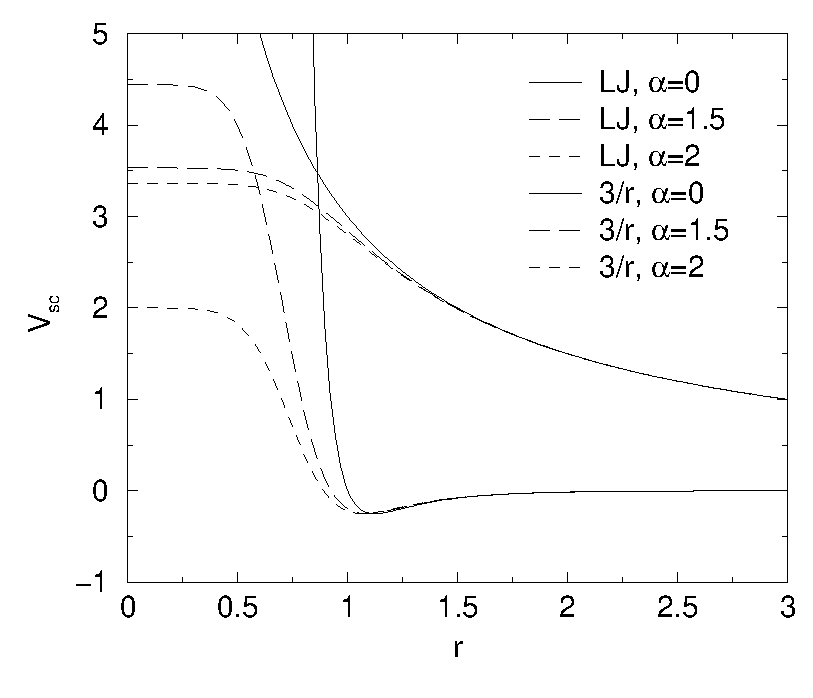
\includegraphics[height=6cm]{plots/softcore}}
\caption{Soft-core interactions at $\LAM=0.5$, with $p=2$ and
$C_6^A=C_{12}^A=C_6^B=C_{12}^B=1$.}
\label{fig:softcore}
\end{figure}
In a free-energy calculation where particles grow out of nothing, or 
particles disappear, using the the simple linear interpolation of the 
Lennard-Jones and Coulomb potentials as described in Equations~\ref{eq:dVljdlambda}
and \ref{eq:dVcoulombdlambda} may lead to poor convergence: when the particles have nearly disappeared, or are close to appearing (at $\LAM$ close to 0 or 1), the interaction energy will be weak enough for particles to get very 
close to each other, leading to large fluctuations in the measured values of 
$\partial V/\partial \LAM$ (which, because of the simple linear 
interpolation, depends on the potentials at both the endpoints of $\LAM$).

To circumvent these problems, the singularities in the potentials need to be removed. This can be done by modifying the regular Lennard-Jones and Coulomb potentials with `soft-core' potentials that limit the energies and forces 
involved at $\LAM$ values between 0 and 1, but not \emph{at} $\LAM=0$ 
or 1.

In {\gromacs} the soft-core potentials $V_{sc}$ are shifted versions of the
regular potentials, so that the singularity in the potential and its
derivatives at $r=0$ is never reached:
\bea
V_{sc}(r) &=& \LL V^A(r_A) + \LAM V^B(r_B)
    \\
r_A &=& \left(\alpha \sigma_A^6 \LAM^p + r^6 \right)^\frac{1}{6}
    \\
r_B &=& \left(\alpha \sigma_B^6 \LL^p + r^6 \right)^\frac{1}{6}
\eea
where $V^A$ and $V^B$ are the normal `hard core' Van der Waals or
electrostatic potentials in state A ($\LAM=0$) and state B ($\LAM=1$)
respectively, $\alpha$ is the soft-core parameter (set with {\tt sc\_alpha} 
in the {\tt .mdp} file), $p$ is the soft-core $\LAM$ power (set with 
{\tt sc\_power}), $\sigma$ is the radius of the interaction, which is 
$(C_{12}/C_6)^{1/6}$ or an input parameter ({\tt sc\_sigma}) when $C_6$ 
or $C_{12}$ is zero.


For intermediate $\LAM$, $r_A$ and $r_B$ alter the interactions very little
for $r > \alpha^{1/6} \sigma$ and quickly switch the soft-core
interaction to an almost constant value for smaller $r$ (\figref{softcore}). 
The force is:
\beq
F_{sc}(r) = -\frac{\partial V_{sc}(r)}{\partial r} =
 \LL F^A(r_A) \left(\frac{r}{r_A}\right)^5 +
\LAM F^B(r_B) \left(\frac{r}{r_B}\right)^5
\eeq
where $F^A$ and $F^B$ are the 'hard core' forces.
The contribution to the derivative of the free energy is:
\bea
\dvdl{V_{sc}(r)} & = &
 V^B(r_B) -V^A(r_A)  + 
	\LL \frac{\partial V^A(r_A)}{\partial r_A}
		   \frac{\partial r_A}{\partial \LAM} + 
	\LAM\frac{\partial V^B(r_B)}{\partial r_B}
		   \frac{\partial r_B}{\partial \LAM}
\nonumber\\
&=&
 V^B(r_B) -V^A(r_A)  + \nonumber \\
 & &
 \frac{p \alpha}{6}
       \left[ \LAM F^B(r_B) r^{-5}_B \sigma_B^6 \LL^{p-1} -
	       \LL F^A(r_A) r^{-5}_A \sigma_A^6 \LAM^{p-1} \right]
\eea

The original GROMOS Lennard-Jones soft-core function~\cite{Beutler94}
uses $p=2$, but $p=1$ gives a smoother $\partial H/\partial\LAM$ curve.
When the changes between the two states involve both the disappearing
and appearing of atoms, it is important that the overlapping of atoms
happens around $\LAM=0.5$. This can usually be achieved with
$\alpha$$\approx0.7$ for $p=1$ and $\alpha$$\approx1.5$ for $p=2$.

Another issue which should be considered is the soft-core effect of hydrogens
without Lennard-Jones interaction. Their soft-core $\sigma$ is
set with {\tt sc\_sigma} in the {\tt .mdp} file. These hydrogens
produce peaks in $\partial H/\partial\LAM$ at $\LAM$ is 0 and/or 1 for $p=1$
and close to 0 and/or 1 with $p=2$. Lowering {\tt sc\_sigma} will decrease
this effect, but it will also increase the interactions with hydrogens
relative to the other interactions in the soft-core state.
} % Brace matches ifthenelse test for gmxlite

\ifthenelse{\equal{\gmxlite}{1}}{}{
\section{Methods}
\subsection{Exclusions and 1-4 Interactions.}
Atoms within a molecule that are close by in the chain, 
{\ie} atoms that are covalently bonded, or linked by one respectively two
atoms are so-called {\em first neighbors, second neighbors} and 
{\em \swapindex{third}{neighbor}s}, (see \figref{chain}). Since the
interactions of atom {\bf i} with atoms {\bf i+1} and {\bf i+2} 

\begin{figure}
\centerline{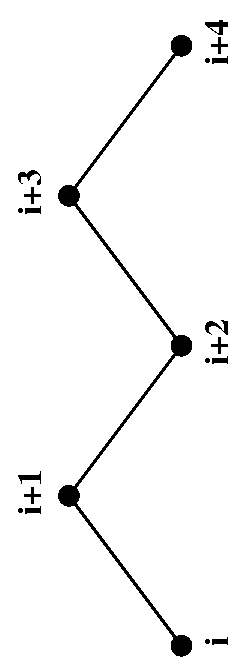
\includegraphics[angle=270,width=8cm]{plots/chain}}
\caption{Atoms along an alkane chain.}
\label{fig:chain}
\end{figure}

are mainly
quantum mechanical, they can not be modeled by a Lennard-Jones potential.
Instead it is assumed that these interactions are adequately modeled
by a harmonic bond term or constraint ({\bf i, i+1}) and a harmonic angle term
({\bf i, i+2}). The first and second neighbors (atoms {\bf i+1} and {\bf i+2}) 
are therefore
{\em excluded} from the Lennard-Jones \swapindex{interaction}{list} 
of atom {\bf i};
atoms {\bf i+1} and {\bf i+2} are called {\em \normindex{exclusions}} of atom {\bf i}.

For third neighbors the normal Lennard-Jones repulsion is sometimes
still too strong, which means that when applied to a molecule the
molecule would deform or break due to the internal strain. This is
especially the case for carbon-carbon interactions in a {\em
cis}-conformation ({\eg} {\em cis}-butane).  Therefore for some of these
interactions the Lennard-Jones repulsion has been reduced in the
{\gromos} force field, which is implemented by keeping a separate list of
1-4 and normal Lennard-Jones parameters. In other force fields, such
as OPLS~\cite{Jorgensen88}, the standard Lennard-Jones parameters are reduced
by a factor of two, but in that case also the dispersion (r$^{-6}$)
and the coulomb interaction are scaled.
{\gromacs} can use either of these methods.

\subsection{Charge Groups}
\label{sec:cg}
\index{charge group}
In principle the force calculation in MD is an $O(N^2)$ problem.
Therefore we apply a \normindex{cut-off} for non-bonded force (NBF)
calculations: only the particles within a certain distance of each
other are interacting. This reduces the cost to $O(N)$ (typically
$100N$ to $200N$) of the NBF. It also introduces an error, which is,
in most cases, acceptable, except when applying the cut-off implies
the creation of charges, in which case you should consider using the
lattice sum methods provided by {\gromacs}.

Consider a water molecule interacting with another atom. When we would apply
the cut-off on an atom-atom basis we might include the atom-Oxygen
interaction (with a charge of -0.82) without the compensating charge
of the protons and so induce a large dipole moment over the system.
Therefore we have to keep groups of atoms with total charge
0 together. These groups are called {\em charge groups}.

\subsection{Treatment of Cut-offs}
\newcommand{\rs}{$r_{short}$}
\newcommand{\rl}{$r_{long}$}
{\gromacs} is quite flexible in treating cut-offs, which implies
there can be quite a number of parameters to set. These parameters are
set in the input file for grompp. There are two sort of parameters
that affect the cut-off interactions; you can select which type
of interaction to use in each case, and which cut-offs should be
used in the neighbor searching.

For both Coulomb and van der Waals interactions there are interaction
type selectors (termed {\tt vdwtype} and {\tt coulombtype}) and two
parameters, for a total of six non-bonded interaction parameters. See
\secref{mdpopt} for a complete description of these parameters.

The neighbor searching (NS) can be performed using a single-range, or a twin-range 
approach. Since the former is merely a special case of the latter we will 
discuss the more general twin-range. In this case NS is described by two
radii {\tt rlist} and max({\tt rcoulomb},{\tt rvdw}).
Usually one builds the neighbor list every 10 time steps
or every 20 fs (parameter {\tt nstlist}). In the neighbor list all interaction 
pairs that  fall within {\tt rlist} are stored. Furthermore, the 
interactions between pairs that do not
fall within {\tt rlist} but do fall within max({\tt rcoulomb},{\tt rvdw})
are computed during NS, and the
forces and energy are stored separately, and added to short-range forces
at every time step between successive NS. If {\tt rlist} = 
max({\tt rcoulomb},{\tt rvdw}), no forces
are evaluated during neighbor list generation.
The \normindex{virial} is calculated from the sum of the short- and
long-range forces.
This means that the virial can be slightly asymmetrical at non-NS steps.
In single precision the virial is almost always asymmetrical, because the
off-diagonal elements are about as large as each element in the sum.
In most cases this is not really a problem, since the fluctuations in the
virial can be 2 orders of magnitude larger than the average.

Except for the plain cut-off,
all of the interaction functions in \tabref{funcparm}
require that neighbor searching is done with a larger radius than the $r_c$
specified for the functional form, because of the use of charge groups.
The extra radius is typically of the order of 0.25 nm (roughly the 
largest distance between two atoms in a charge group plus the distance a 
charge group can diffuse within neighbor list updates).

%If your charge groups are very large it may be interesting to turn off charge
%groups, by setting the option 
%{\tt bAtomList = yes} in your {\tt grompp.mdp} file.
%In this case only a small extra radius to account for diffusion needs to be 
%added (0.1 nm). Do not however use this together with the plain cut-off
%method, as it will generate large artifacts (\secref{cg}).
%In summary, there are four parameters that describe NS behavior:
%{\tt nstlist} (update frequency in number of time steps),
%{\tt bAtomList} (whether or not charge groups are used to generate neighbor list, the default is to use charge groups, so {\tt bAtomList = no}),
%{\tt rshort} and {\tt rlong} which are the two radii {\rs} and {\rl}
%described above.

\begin{table}[ht]
\centering
\begin{tabular}{|ll|l|}
\dline
\multicolumn{2}{|c|}{Type}              & Parameters            \\
\hline
Coulomb&Plain cut-off   & $r_c$, $\epsr$        \\
&Reaction field         & $r_c$, $\epsrf$       \\
&Shift function         & $r_1$, $r_c$, $\epsr$         \\
&Switch function        & $r_1$, $r_c$, $\epsr$         \\
\hline
VdW&Plain cut-off       & $r_c$         \\
&Shift function         & $r_1$, $r_c$          \\
&Switch function        & $r_1$, $r_c$          \\
\dline
\end{tabular}
\caption[Parameters for the different functional forms of the
non-bonded interactions.]{Parameters for the different functional
forms of the non-bonded interactions.}
\label{tab:funcparm}
\end{table}
} % Brace matches ifthenelse test for gmxlite


\newcommand{\vvis}{\ve{r}_s}
\newcommand{\Fi}{\ve{F}_i'}
\newcommand{\Fj}{\ve{F}_j'}
\newcommand{\Fk}{\ve{F}_k'}
\newcommand{\Fl}{\ve{F}_l'}
\newcommand{\Fvis}{\ve{F}_{s}}
\newcommand{\rvik}{\ve{r}_{ik}}
\newcommand{\rvis}{\ve{r}_{is}}
\newcommand{\rvjk}{\ve{r}_{jk}}
\newcommand{\rvjl}{\ve{r}_{jl}}

\ifthenelse{\equal{\gmxlite}{1}}{}{
\section{Virtual interaction-sites}
\label{sec:virtual_sites}
\index{virtual interaction-sites}
Virtual interaction-sites (called \seeindex{dummy atoms}{virtual interaction-sites} in {\gromacs} versions before 3.3)
can be used in {\gromacs} in a number of ways. 
We write the position of the virtual site $\ve{r}_s$ as a function of
the positions of other particles \ve{r}$_i$: $\ve{r}_s =
f(\ve{r}_1..\ve{r}_n)$. The virtual site, which may carry charge, or can be
involved in other interactions can now be used in the force
calculation.  The force acting on the virtual site must be
redistributed over the particles with mass in a consistent way.
A good way to do this can be found in ref.~\cite{Berendsen84b}.
We can write the potential energy as
\beq
V = V(\vvis,\ve{r}_1,\ldots,\ve{r}_n) = V^*(\ve{r}_1,\ldots,\ve{r}_n)
\eeq
The force on the particle $i$ is then
\beq
\ve{F}_i = -\frac{\partial V^*}{\partial \ve{r}_i} 
         = -\frac{\partial V}{\partial \ve{r}_i} - 
            \frac{\partial V}{\partial \vvis} 
            \frac{\partial \vvis}{\partial \ve{r}_i}
         = \ve{F}_i^{direct} + \Fi
\eeq
the first term of which is the normal force. 
The second term is the force on particle $i$ due to the virtual site, which
can be written in tensor notation:
\newcommand{\partd}[2]{\displaystyle\frac{\partial #1}{\partial #2_i}}
\beq
\Fi = \left[\begin{array}{ccc}
\partd{x_s}{x} & \partd{y_s}{x} & \partd{z_s}{x}        \\[1ex]
\partd{x_s}{y} & \partd{y_s}{y} & \partd{z_s}{y}        \\[1ex]
\partd{x_s}{z} & \partd{y_s}{z} & \partd{z_s}{z}
\end{array}\right]\Fvis
\label{eqn:fvsite}
\eeq
where $\Fvis$ is the force on the virtual site and $x_s$, $y_s$ and
$z_s$ are the coordinates of the virtual site. In this way the total
force and the total torque are conserved~\cite{Berendsen84b}.

As a further note, the computation of the \normindex{virial}
(\eqnref{Xi}) is non-trivial when virtual sites are used. Since the
virial involves a summation over all the atoms (rather than virtual
sites) the forces most be redistributed from the virtual sites to the
atoms (using ~\eqnref{fvsite}) {\em before} computation of the
virial. In some special cases where the forces on the atoms can be
written as a linear combination of the forces on the virtual sites (types 2
and 3 below) there is no difference between computing the virial
before and after the redistribution of forces.  However, in the
general case redistribution should be done first.

\begin{figure}
\centerline{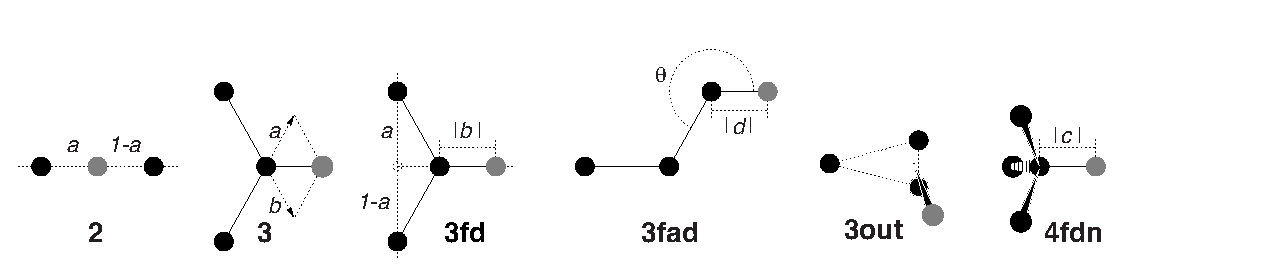
\includegraphics[width=15cm]{plots/dummies}}
\caption[Virtual site construction.]{The six different types of virtual
site construction in \protect{\gromacs}. The constructing atoms are
shown as black circles, the virtual sites in gray.}
\label{fig:vsites}
\end{figure}

There are six ways to construct virtual sites from surrounding atoms in
{\gromacs}, which we classify by the number of constructing
atoms. Note that all site types mentioned can be constructed from
types 3fd (normalized, in-plane) and 3out (non-normalized, out of
plane). However, the amount of computation involved increases sharply
along this list, so we strongly recommended using the first adequate
virtual site type that will be sufficient for a certain purpose.
\figref{vsites} depicts 6 of the available virtual site constructions.
The conceptually simplest construction types are linear combinations:
\beq
\vvis = \sum_{i=1}^N w_i \, \ve{r}_i
\eeq
The force is then redistributed using the same weights:
\beq
\Fi = w_i \, \Fvis
\eeq

The types of virtual sites supported in {\gromacs} are given in the list below.
Constructing atoms in virtual sites can be virtual sites themselves, but
only if they are higher in the list, i.e. virtual sites can be
constructed from ``particles'' that are simpler virtual sites.
\begin{itemize}
\item[{\bf\sf 2.}]As a linear combination of two atoms
        (\figref{vsites} 2):
\beq
        w_i = 1 - a ~,~~ w_j = a
\eeq
        In this case the virtual site is on the line through atoms $i$ and
        $j$.

\item[{\bf\sf 3.}]As a linear combination of three atoms
        (\figref{vsites} 3):
\beq
        w_i = 1 - a - b ~,~~ w_j = a ~,~~ w_k = b
\eeq
        In this case the virtual site is in the plane of the other three
	particles.

\item[{\bf\sf 3fd.}]In the plane of three atoms, with a fixed distance
        (\figref{vsites} 3fd):
\beq
        \vvis ~=~ \ve{r}_i + b \frac{  \rvij + a \rvjk  }
                                    {| \rvij + a \rvjk |}      
\eeq
        In this case the virtual site is in the plane of the other three
        particles at a distance of $|b|$ from $i$.
        The force on particles $i$, $j$ and $k$ due to the force on the virtual
        site can be computed as:
\beq
        \begin{array}{lcr}
        \Fi &=& \displaystyle \Fvis - \gamma ( \Fvis - \ve{p} ) \\[1ex]
        \Fj &=& \displaystyle (1-a)\gamma (\Fvis - \ve{p})      \\[1ex]
        \Fk &=& \displaystyle a \gamma (\Fvis - \ve{p})         \\
        \end{array}
        ~\mbox{~ where~ }~
        \begin{array}{c}
\displaystyle \gamma = \frac{b}{| \rvij + a \rvjk |} \\[2ex]
\displaystyle \ve{p} = \frac{ \rvis \cdot \Fvis }
                      { \rvis \cdot \rvis } \rvis
        \end{array}
\eeq

\item[{\bf\sf 3fad.}]In the plane of three atoms, with a fixed angle and
        distance (\figref{vsites} 3fad):
\beq
\label{eqn:vsite2fad-F}
         \vvis ~=~ \ve{r}_i +
                    d \cos \theta \frac{\rvij}{|\rvij|} +
                    d \sin \theta \frac{\ve{r}_\perp}{|\ve{r}_\perp|}
        ~\mbox{~ where~ }~
        \ve{r}_\perp ~=~ \rvjk - 
                        \frac{ \rvij \cdot \rvjk }
                             { \rvij \cdot \rvij }
                         \rvij
\eeq
        In this case the virtual site is in the plane of the other three
        particles at a distance of $|d|$ from $i$ at an angle of
        $\alpha$ with $\rvij$. Atom $k$ defines the plane and the
        direction of the angle. Note that in this case $b$ and
        $\alpha$ must be specified, instead of $a$ and $b$ (see also
        \secref{vsitetop}). The force on particles $i$, $j$ and $k$
        due to the force on the virtual site can be computed as (with
        $\ve{r}_\perp$ as defined in \eqnref{vsite2fad-F}):
\newcommand{\dfrac}{\displaystyle\frac}
\beq
\begin{array}{c}
        \begin{array}{lclllll}
        \Fi &=& \Fvis &-& 
                \dfrac{d \cos \theta}{|\rvij|} \ve{F}_1 &+&
                \dfrac{d \sin \theta}{|\ve{r}_\perp|} \left( 
                \dfrac{ \rvij \cdot \rvjk }
                     { \rvij \cdot \rvij } \ve{F}_2     +
                \ve{F}_3 \right)                                \\[3ex]
        \Fj &=& &&
                \dfrac{d \cos \theta}{|\rvij|} \ve{F}_1 &-&
                \dfrac{d \sin \theta}{|\ve{r}_\perp|} \left(
                 \ve{F}_2 + 
                 \dfrac{ \rvij \cdot \rvjk }
                        { \rvij \cdot \rvij } \ve{F}_2 +
                \ve{F}_3 \right)                                \\[3ex]
        \Fk &=& && &&
                \dfrac{d \sin \theta}{|\ve{r}_\perp|} \ve{F}_2  \\[3ex]
        \end{array}                                             \\[5ex]
        \mbox{where ~}
        \ve{F}_1 = \Fvis -
                  \dfrac{ \rvij \cdot \Fvis }
                        { \rvij \cdot \rvij } \rvij
        \mbox{\,, ~}
        \ve{F}_2 = \ve{F}_1 -
                  \dfrac{ \ve{r}_\perp \cdot \Fvis }
                        { \ve{r}_\perp \cdot \ve{r}_\perp } \ve{r}_\perp
        \mbox{~and ~}
        \ve{F}_3 = \dfrac{ \rvij \cdot \Fvis }
                         { \rvij \cdot \rvij } \ve{r}_\perp
\end{array}
\eeq

\item[{\bf\sf 3out.}]As a non-linear combination of three atoms, out of plane
        (\figref{vsites} 3out):
\beq
        \vvis ~=~ \ve{r}_i + a \rvij + b \rvik +
                c (\rvij \times \rvik)
\eeq
        This enables the construction of virtual sites out of the plane of the
        other atoms.
        The force on particles $i,j$ and $k$ due to the force on the virtual
        site can be computed as:
\beq
\begin{array}{lcl}
\vspace{4mm}
\Fj &=& \left[\begin{array}{ccc}
 a              &  -c\,z_{ik}   & c\,y_{ik}     \\[0.5ex]
 c\,z_{ik}      &   a           & -c\,x_{ik}    \\[0.5ex]
-c\,y_{ik}      &   c\,x_{ik}   & a
\end{array}\right]\Fvis                                 \\
\vspace{4mm}
\Fk &=& \left[\begin{array}{ccc}
 b              &   c\,z_{ij}   & -c\,y_{ij}    \\[0.5ex]
-c\,z_{ij}      &   b           & c\,x_{ij}     \\[0.5ex]
 c\,y_{ij}      &  -c\,x_{ij}   & b
\end{array}\right]\Fvis                                 \\
\Fi &=& \Fvis - \Fj - \Fk
\end{array}
\eeq

\item[{\bf\sf 4fd.}]From four atoms, with a fixed distance
        (\figref{vsites} 4fd):
\beq
        \vvis ~=~ \ve{r}_i + c \frac{  \rvij + a \rvjk + b \rvjl }
                                    {| \rvij + a \rvjk + b \rvjl|}     
\eeq
        In this case the virtual site is at a distance of $|c|$ from $i$.
        The force on particles $i$, $j$, $k$ and $l$ due to the force 
        on the virtual site can be computed as:
\beq
        \begin{array}{lcr}
        \Fi &=& \displaystyle \Fvis - \gamma ( \Fvis - \ve{p} ) \\[1ex]
        \Fj &=& \displaystyle (1-a-b)\gamma (\Fvis - \ve{p})    \\[1ex]
        \Fk &=& \displaystyle a \gamma (\Fvis - \ve{p})         \\[1ex]
        \Fl &=& \displaystyle b \gamma (\Fvis - \ve{p})         \\
        \end{array}
        ~\mbox{~ where~ }~
        \begin{array}{c}
\displaystyle \gamma = \frac{c}{| \rvij + a \rvjk + b \rvjl |} \\[2ex]
\displaystyle \ve{p} = \frac{ \rvis \cdot \Fvis }
                      { \rvis \cdot \rvis } \rvis
        \end{array}
\eeq

\item[{\bf\sf N.}] A linear combination of $N$ atoms with relative
weights $a_i$. The weight for atom $i$ is:
\beq
  w_i = a_i \left(\sum_{j=1}^N a_j \right)^{-1}
\eeq
There are three options for setting the weights:
\begin{itemize}
\item[COG] center of geometry: equal weights
\item[COM] center of mass: $a_i$ is the mass of atom $i$;
when in free-energy simulations the mass of the atom is changed,
only the mass of the A-state is used for the weight
\item[COW] center of weights: $a_i$ is defined by the user
\end{itemize}

\end{itemize}
} % Brace matches ifthenelse test for gmxlite

\newcommand{\dr}{{\rm d}r}
\newcommand{\avcsix}{\left< C_6 \right>}

\ifthenelse{\equal{\gmxlite}{1}}{}{
\section{Dispersion correction}
\index{dispersion correction}
In this section we derive long range corrections due to the use of a
cut-off for Lennard Jones or Buckingham interactions.
We assume that the cut-off is
so long that the repulsion term can safely be neglected, and therefore
only the dispersion term is taken into account. Due to the nature of
the dispersion interaction, energy and pressure corrections both are
negative. While the energy correction is usually small, it may be
important for free energy calculations. The pressure correction in
contrast is very large and can not be neglected. Although it is in
principle possible to parameterize a force field such that the pressure
is close to 1 bar even without correction, such a method makes the
parameterization dependent on the cut-off and is therefore
undesirable. Please note that it is not consistent to use the long
range correction to the dispersion without using either a
\normindex{reaction field} method or a proper long range
electrostatics method such as Ewald summation or PPPM.

\subsection{Energy}
\label{sec:ecorr}
The long range contribution of the dispersion interaction to the
virial can be derived analytically, if we assume a homogeneous
system beyond the cut-off distance $r_c$. The dispersion energy
between two particles is written as:
\beq
V(\rij)	~=~	- C_6\,\rij^{-6}
\eeq
and the corresponding force is
\beq
\Fvij	~=~	- 6\,C_6\,\rij^{-8}\rvij
\eeq
In a periodic system it is not easy to calculate the full potentials,
so usually a cut-off is applied, which can be abrupt or smooth.
We will call the potential and force with cut-off $V_c$ and $\ve{F}_c$.
The long-range contribution to the dispersion energy
in a system with $N$ particles and particle density $\rho$ = $N/V$ is:
\beq
\label{eqn:enercorr}
V_{lr}  ~=~ \half N \rho\int_0^{\infty}   4\pi r^2 g(r) \left( V(r) -V_c(r) \right) {\dr}
\eeq
We will integrate this for the shift function, which is the most general
form of Van der Waals interaction available in {\gromacs}.
The shift function has a constant difference $S$ from 0 to $r_1$
and is 0 beyond the cut-off distance $r_c$.
We can integrate \eqnref{enercorr} assuming that the density in the sphere
within $r_1$ is equal to the global density and
the radial distribution function $g(r)$ is 1 beyond $r_1$:
\bea
\nonumber
V_{lr}  &=& \half N \left(
  \rho\int_0^{r_1}  4\pi r^2 g(r) \, C_6 \,S\,{\dr}
+ \rho\int_{r_1}^{r_c}  4\pi r^2 \left( V(r) -V_c(r) \right) {\dr}
+ \rho\int_{r_c}^{\infty}  4\pi r^2 V(r) \, {\dr}
\right) \\
& = & \half N \left(\left(\frac{4}{3}\pi \rho r_1^{3} - 1\right) C_6 \,S
+ \rho\int_{r_1}^{r_c} 4\pi r^2 \left( V(r) -V_c(r) \right) {\dr}
-\frac{4}{3} \pi N \rho\, C_6\,r_c^{-3}
\right)
\eea
where the term $-1$ corrects for the self-interaction.
For a plain cut-off we only need to assume that $g(r)$ is 1 beyond $r_c$
and the correction reduces to~\cite{Allen87}:
\bea
V_{lr} & = & -\frac{2}{3} \pi N \rho\, C_6\,r_c^{-3}
\eea
If we consider for example a box of pure water, simulated with a cut-off
of 0.9 nm and a density of 1 g cm$^{-3}$ this correction is 
-0.75 kJ mol$^{-1}$ per molecule.

For a homogeneous mixture we need to define 
an {\em average dispersion constant}:
\beq
\label{eqn:avcsix}
\avcsix	= \frac{2}{N(N-1)}\sum_i^N\sum_{j>i}^N C_6(i,j)\\
\eeq
In {\gromacs} excluded pairs of atoms do not contribute to the average.

In the case of inhomogeneous simulation systems, {\eg} a system with a
lipid interface, the energy correction can be applied if 
$\avcsix$ for both components is comparable.

\subsection{Virial and pressure}
The scalar virial of the system due to the dispersion interaction between
two particles $i$ and $j$ is given by:
\beq
\Xi	~=~	-\half \rvij \cdot \Fvij ~=~	3\,C_6\,\rij^{-6}
\eeq
The pressure is given by:
\beq
P	~=~	\frac{2}{3\,V}\left(E_{kin} - \Xi\right)
\eeq
The long-range correction to the virial is given by:
\beq
\Xi_{lr} ~=~ \half N \rho \int_0^{\infty} 4\pi r^2 g(r) (\Xi -\Xi_c) \,\dr
\eeq
We can again integrate the long range contribution to the 
virial assuming $g(r)$ is 1 beyond $r_1$:
\bea
\Xi_{lr}&=&	\half N \rho \left(
    \int_{r_1}^{r_c}  4 \pi r^2 (\Xi -\Xi_c)  \,\dr
  + \int_{r_c}^{\infty} 4 \pi r^2 3\,C_6\,\rij^{-6}\,  \dr
\right)	\nonumber\\
        &=&     \half N \rho \left(
    \int_{r_1}^{r_c} 4 \pi r^2 (\Xi -\Xi_c) \, \dr
  + 4 \pi C_6 \, r_c^{-3} \right)
\eea
For a plain cut-off the correction to the pressure is~\cite{Allen87}:
\beq
P_{lr}	~=~	-\frac{4}{3} \pi C_6\, \rho^2 r_c^{-3}
\eeq
Using the same example of a water box, the correction to the virial is
0.75 kJ mol$^{-1}$ per molecule,
the corresponding correction to the pressure for 
SPC water is approximately -280 bar.

For homogeneous mixtures we can again use the average dispersion constant
$\avcsix$ (\eqnref{avcsix}):
\beq
P_{lr}	~=~	-\frac{4}{3} \pi \avcsix \rho^2 r_c^{-3}
\label{eqn:pcorr}
\eeq
For inhomogeneous systems \eqnref{pcorr} can be applied under the same
restriction as holds for the energy (see \secref{ecorr}).
} % Brace matches ifthenelse test for gmxlite

\ifthenelse{\equal{\gmxlite}{1}}{}{
\section{Long Range Electrostatics}
\label{sec:lr_elstat}
\subsection{\normindex{Ewald sum}mation}
\label{sec:ewald}
The total electrostatic energy of $N$ particles and the periodic
images\index{periodic boundary conditions} are given by
\begin{equation}
V=\frac{f}{2}\sum_{n_x}\sum_{n_y}
\sum_{n_{z}*} \sum_{i}^{N} \sum_{j}^{N} 
\frac{q_i q_j}{{\bf r}_{ij,{\bf n}}}.
\label{eqn:totalcoulomb}
\end{equation}
$(n_x,n_y,n_z)={\bf n}$ is the box index vector, and the star indicates that
terms with $i=j$ should be omitted when $(n_x,n_y,n_z)=(0,0,0)$. The
distance ${\bf r}_{ij,{\bf n}}$ is the real distance between the charges and
not the minimum-image. This sum is conditionally convergent, but 
very slow.

Ewald summation was first introduced as a method to calculate
long-range interactions of the periodic images in
crystals~\cite{Ewald21}. The idea is to convert the single
slowly-converging sum \eqnref{totalcoulomb} into two
quickly-converging terms and a constant term:
\begin{eqnarray}
V &=& V_{dir} + V_{rec} + V_{0} \\[0.5ex]
V_{dir} &=& \frac{f}{2} \sum_{i,j}^{N} 
\sum_{n_x}\sum_{n_y}
\sum_{n_{z}*} q_i q_j \frac{\mbox{erfc}(\beta {r}_{ij,{\bf n}} )}{{r}_{ij,{\bf n}}} \\[0.5ex]
V_{rec} &=& \frac{f}{2 \pi V} \sum_{i,j}^{N} q_i q_j 
\sum_{m_x}\sum_{m_y}
\sum_{m_{z}*} \frac{\exp{\left( -(\pi {\bf m}/\beta)^2 + 2 \pi i
      {\bf m} \cdot ({\bf r}_i - {\bf r}_j)\right)}}{{\bf m}^2} \\[0.5ex]
V_{0} &=& -\frac{f \beta}{\sqrt{\pi}}\sum_{i}^{N} q_i^2,
\end{eqnarray}
where $\beta$ is a parameter that determines the relative weight of the
direct and reciprocal sums and ${\bf m}=(m_x,m_y,m_z)$.
In this way we can use a short cut-off (of the order of $1$~nm) in the direct space sum and a
short cut-off in the reciprocal space sum ({\eg} 10 wave vectors in each 
direction). Unfortunately, the computational cost of the reciprocal
part of the sum increases as $N^2$
(or $N^{3/2}$ with a slightly better algorithm) and it is therefore not 
realistic for use in large systems.

\subsubsection{Using Ewald}
Don't use Ewald unless you are absolutely sure this is what you want -
for almost all cases the PME method below will perform much better.
If you still want to employ classical Ewald summation enter this in
your {\tt .mdp} file, if the side of your box is about $3$~nm:

\begin{tt}
coulombtype     = Ewald\\
rvdw            = 0.9\\
rlist           = 0.9\\
rcoulomb        = 0.9\\
fourierspacing  = 0.6\\
ewald\_rtol      = 1e-5\\
\end{tt}

The {\tt fourierspacing} parameter times the box dimensions determines
the highest magnitude of wave vectors $m_x,m_y,m_z$ to use in each
direction. With a 3~nm cubic box this example would use $11$ wave vectors
(from $-5$ to $5$) in each direction.  The {\tt ewald\_rtol} parameter
is the relative strength of the electrostatic interaction at the
cut-off. Decreasing this gives you a more accurate direct sum, but a
less accurate reciprocal sum.
 
\subsection{\normindex{PME}}
\label{sec:pme}
Particle-mesh Ewald is a method proposed by Tom
Darden~\cite{Darden93,Essmann95} to improve the performance of the
reciprocal sum. Instead of directly summing wave vectors, the charges
are assigned to a grid using cardinal B-spline interpolation. This
grid is then Fourier transformed with a 3D FFT algorithm and the
reciprocal energy term obtained by a single sum over the grid in
k-space.

The potential at the grid points is calculated by inverse
transformation, and by using the interpolation factors we get the
forces on each atom. 

The PME algorithm scales as $N \log(N)$, and is substantially faster
than ordinary Ewald summation on medium to large systems. On very
small systems it might still be better to use Ewald to avoid the
overhead in setting up grids and transforms.
For the parallelization of PME see the section on MPMD PME (\ssecref{mpmd_pme}).

\subsubsection{Using PME}
To use Particle-mesh Ewald summation in {\gromacs}, specify the
following lines in your {\tt .mdp} file:

\begin{tt}
coulombtype     = PME\\
rvdw            = 0.9\\
rlist           = 0.9\\
rcoulomb        = 0.9\\
fourierspacing  = 0.12\\
pme\_order       = 4\\
ewald\_rtol      = 1e-5\\
\end{tt}

In this case the {\tt fourierspacing} parameter determines the maximum
spacing for the FFT grid and {\tt pme\_order} controls the
interpolation order. Using fourth-order (cubic) interpolation and this
spacing should give electrostatic energies accurate to about
$5\cdot10^{-3}$. Since the Lennard-Jones energies are not this
accurate it might even be possible to increase this spacing slightly.

Pressure scaling works with PME, but be aware of the fact that
anisotropic scaling can introduce artificial ordering in some systems.

\subsection{\normindex{PPPM}}
\label{sec:pppm}
The \seeindex{Particle-Particle Particle-Mesh}{PPPM} methods of
Hockney \& Eastwood can also be applied in {\gromacs} for the
treatment of long range electrostatic
interactions~\cite{Hockney81,Darden93,Luty95a}.  With this algorithm
the charges of all particles are spread over a grid of dimensions
($n_x$,$n_y$,$n_z$) using a weighting function called the
triangle-shaped charged distribution:
\beq
\begin{array}{lcl}
W(\ve{r}) &=&   W(x)~W(y)~W(z)  \\[1ex]
W(\xi)  &=& \left\{
\begin{array}{ll}
\frac{3}{4} - \left(\frac{\xi}{h}\right)^2 
        & |\xi| \leq \frac{h}{2}                                \\[0.5ex]
\frac{1}{2}\left(\frac{3}{2} - \frac{|\xi|}{h}\right)^2 
        & \frac{h}{2} < |\xi| < \frac{3h}{2}                    \\[0.5ex]
0       & \frac{3h}{2} \leq |\xi|                               \\[0.5ex]
\end{array}
\right.
\end{array}
\eeq
where $\xi$ (is x, y or z) is the distance to a grid point in the corresponding
dimension. Only the 27 closest grid points need to be taken into account for each charge.

Then, this charge distribution is Fourier transformed using a 3D inverse FFT 
routine.
In Fourier space a convolution with function $\hat{G}$ is performed:
\beq
\hat{G}(k)      ~=~     \frac{\hat{g}(k)}{\epsilon_0 k^2}
\eeq
where $\hat{g}$ is the Fourier transform of the charge spread function
g(r). This yield the long range potential $\hat{\phi}(k)$ on the mesh, which
can be transformed using a forward FFT routine into the real space potential.
Finally the potential and forces are retrieved using interpolation~\cite{Luty95a}.
%
% note - this accuracy is just a rough estimate...
%
It is not easy to calculate the full long-range virial tensor with
PPPM, but it is possible to obtain the trace. This means that the sum
of the pressure components is correct (and therefore the isotropic
pressure) but not necessarily the individual pressure components!

\subsubsection{Using PPPM}
To use the PPPM algorithm in {\gromacs}, specify the
following lines in your {\tt .mdp} file:

\begin{tt}
coulombtype     = PPPM\\
rlist           = 1.0\\
rcoulomb        = 0.85\\
rcoulomb\_switch = 0.0\\
rvdw            = 1.0\\
fourierspacing  = 0.075\\
\end{tt}

For details on the switch parameters see the section on modified
long-range interactions in this manual. When using PPPM we recommend
to take at most 0.075 nm per grid point ({\eg} 20 grid points for 1.5
nm).  PPPM does not provide the same accuracy as PME but can be
slightly faster in some cases. Due to the problem with the pressure
tensor you shouldn't use it with pressure coupling.

We're somewhat ambivalent about PPPM, so if you use it please contact
us - otherwise it might be removed from future releases so we can concentrate
our efforts on PME.


\subsection{Optimizing Fourier transforms}
To get the best possible performance you should try to avoid large
prime numbers for grid dimensions.
The FFT code used in {\gromacs} is
optimized for grid sizes of the form $2^a 3^b 5^c 7^d 11^e 13^f$,
where $e+f$ is $0$ or $1$ and the other exponents arbitrary. (See
further the documentation of the FFT algorithms at 
\href{http://www.fftw.org}{www.fftw.org}.

It is also possible to optimize the transforms for the current problem
by performing some calculations at the start of the run. This is not
done per default since it takes a couple of minutes, but for large
runs it will save time. Turn it on by specifying

\begin{tt}
optimize\_fft      = yes\\
\end{tt}
in your {\tt .mdp} file.

When running in parallel the grid must be communicated several times
and thus hurting scaling performance. With PME you can improve this
by increasing grid spacing while simultaneously increasing the
interpolation to {\eg} sixth order. 
Since the interpolation is entirely local a this will
improve the scaling in most cases.

%
% Temporarily removed since I am not sure about the state of the testlr 
% program...
%
%It is possible to test the accuracy of your settings using the program 
%{\tt\normindex{testlr}} in the {\tt src/gmxlib} dir. This program computes
%forces and potentials using PPPM and an Ewald implementation and gives the
%absolute and RMS errors in both:
%\begin{tt}
%ERROR ANALYSIS\\
%Error:         Max Abs         RMS\\
%Force            1.132       0.251\\
%Potential        0.113       0.035\\
%\end{tt}
%{\bf Note:} these numbers were generated using a grid spacing of
%0.058 nm and $r_c$ = 1.0 nm.
%
%You can see what the accuracy is without optimizing the
%$\hat{G}(k)$ function, if you pass the {\tt -ghat} option to {\tt
%testlr}. Try it if you think the {\tt mk\_ghat} procedure is a waste
%of time.
} % Brace matches ifthenelse test for gmxlite


%%%%%%%%%%%%%%%%%%%%%%%%%%%%%%%%%%%%%%%%%%%%%%%%%%%%%%%%%%%%%%%%%%%
%%%%%%%%%%%%%%%%%%%%%%%%%%%%%%%%%%%%%%%%%%%%%%%%%%%%%%%%%%%%%%%%%%%
%%%%%%%%%%%%%%%%%%%%%%%%%%%%%%%%%%%%%%%%%%%%%%%%%%%%%%%%%%%%%%%%%%%

\section{Force field\index{force-field}}
\label{sec:ff}
A force field is built up from two distinct components:
\begin{itemize}
\item The set of equations (called the {\em
    \swapindex{potential}{function}s}) used to generate the potential
  energies and their derivatives, the forces. These are described in
  detail in the previous chapter.
\item The parameters used in this set of equations. These are not
  given in this manual, but in the data files corresponding to your
  {\gromacs} distribution.
\end{itemize}
Within one set of equations various sets of parameters can be
used. Care must be taken that the combination of equations and
parameters form a consistent set. It is in general dangerous to make
{\em ad hoc} changes in a subset of parameters, because the various
contributions to the total force are usually interdependent. This
means in principle that every change should be documented, verified by
comparison to experimental data and published in a peer-reviewed
journal before it can be used.

{\gromacs} {\gmxver} includes several force fields, and additional
ones are available on the website. If you do not know which one to
select we recommend Gromos96 for united-atom setups and OPLS-AA/L for
all-atom parameters. That said, we describe the available options in
some detail.

\subsection{GROMOS87\index{gromos-87 force field}}
The \gromosv{87} suite of programs and corresponding force
field\cite{biomos} formed the basis for the development of {\gromacs}
in the early 1990s.  The original GROMOS87 force field is not
available in {\gromacs}. In previous versions ($<$ 3.3.2) there used
to be the so-called {\gromacs} force field which was based on
\gromosv{87}~\cite{biomos}\index{gromos-87}, with a small modification
concerning the interaction between water-oxygens and carbon
atoms~\cite{Buuren93b,Mark94}, as well as 10 extra atom
types~\cite{Jorgensen83,Buuren93a,Buuren93b,Mark94,Liu95}. Whenever
using this force field, please cite the above references, and do not
call it {\gromacs} force field, instead name it
\gromosv{87}~\cite{biomos} with corrections as detailed
in~\cite{Buuren93b,Mark94}.

\subsubsection{\swapindex{All-hydrogen}{force-field}}
The {\gromacs} all-hydrogen force-field is almost identical to the
normal {\gromacs} force field, since the extra hydrogens have no
Lennard-Jones interaction and zero charge. The only differences are in
the bond angle and improper dihedral angle terms. This force field is
only useful when you need the exact hydrogen positions, for instance
for distance restraints derived from NMR measurements. When citing
this force field please read the previous paragraph.

\subsection{\gromosv{96}\index{gromos-96 force field}}
{\gromacs} supports the \gromosv{96} force fields~\cite{gromos96}.
All parameters for the 43a1, 43a2 (development, improved alkane
dihedrals) and 43b1 (vacuum) force fields are included.  All standard
building blocks are included and topologies can be build automatically
by {\tt pdb2gmx}.  The \gromosv{96} force field is a further
development of the \gromosv{87} force field on which the {\gromacs}
force field is based. The \gromosv{96} force field has improvements
over the {\gromacs} force field for proteins and small molecules.
It is not, however, recommended for use with long alkanes and
lipids.  The \gromosv{96} force field differs from the {\gromacs}
force field in a few aspects:
\begin{itemize}
\item the force field parameters
\item the parameters for the bonded interactions are not linked to atom types
\item a fourth power bond stretching potential (\secref{bondpot})
\item an angle potential based on the cosine of the angle (\secref{anglepot})
\end{itemize}
There are two differences in implementation between {\gromacs} and \gromosv{96}
which can lead to slightly different results when simulating the same system
with both packages: 
\begin{itemize}
\item in \gromosv{96} neighbor searching for solvents is performed on the
first atom of the solvent molecule, this is not implemented in {\gromacs},
but the difference with searching with centers of charge groups is very small
\item the virial in \gromosv{96} is molecule-based. This is not implemented in
{\gromacs}, which uses atomic virials
\end{itemize}
The \gromosv{96} force field was parameterized with a Lennard-Jones cut-off
of 1.4 nm, so be sure to use a Lennard-Jones cut-off of at least 1.4.
A larger cut-off is possible, because the Lennard-Jones potential and forces
are almost zero beyond 1.4 nm.

\subsubsection{\gromosv{96} files}\index{gromos-96 files}\index{files,
gromos|see{gromos-96 files}}
{\gromacs} can read and write \gromosv{96} coordinate and trajectory files.
These files should have the extension {\tt .g96}.
Such a file can be a \gromosv{96} initial/final
configuration file or a coordinate trajectory file or a combination of both.
The file is fixed format; all floats are written as 15.9 (files can get huge).
{\gromacs} supports the following data blocks in the given order:
\begin{itemize}
\item Header block:
\begin{tt}
TITLE (mandatory)\\
\end{tt}

\item Frame blocks:
\begin{tt}
TIMESTEP (optional)\\
POSITION/POSITIONRED (mandatory)\\
VELOCITY/VELOCITYRED (optional)\\
BOX (optional)\\
\end{tt}

\end{itemize}
See the \gromosv{96} manual~\cite{gromos96} for a complete description
of the blocks. Note that all {\gromacs} programs can read compressed
(.Z) or gzipped (.gz) files.

\subsection{OPLS/AA\index{OPLS/AA force field}}

\subsection{Amber\index{Amber force field}}

\subsection{CHARMM\index{Charmm force field}}

As of version 4.5, {\gromacs} supports the CHARMM27 force field for proteins~\cite{mackerell04, mackerell98}, lipids~\cite{feller00} and nucleic acids~\cite{foloppe00}. The protein parameters (and to some extent the lipid and nucleic acid parameters) were thoroughly tested -- both by comparing potential energies between the port and the standard parameter set in the CHARMM molecular simulation package, as well by how the protein force field behaves together with {\gromacs}-specific techniques such as virtual sites (enabling long time steps) and a fast implicit solvent recently implemented~\cite{Larsson10} -- and the details and results are presented in the paper by Bjelkmar et al.~\cite{Bjelkmar10}. The nucleic acid parameters, as well as the ones for HEME, were converted and tested by Michel Cuendet.

When selecting the CHARMM force field in \normindex{pdb2gmx} the default option is to use CMAP (dihedral cross terms for protein backbone), use -nocmap flag otherwise.

\subsection{Martini\index{Martini force field}}


% LocalWords:  dihedrals centro ij dV dr LJ lj rcl jj Bertelot OPLS bh bham rf
% LocalWords:  coul defunits grompp crf vcrf fcrf Tironi Debye kgrf cgrf krf dx
% LocalWords:  PPPM der Waals erfc lr elstat chirality bstretch bondpot kT kJ
% LocalWords:  anharmonic morse mol betaij expminx SPC timestep fs FENE ijk kj
% LocalWords:  anglepot CHARMm UB ik rr substituents ijkl Ryckaert Bellemans rb
% LocalWords:  alkanes pdb gmx IUPAC IUB jkl cis rbdih crb kcal cubicspline xvg
% LocalWords:  topfile mdrun posres ar dihr lcllll NMR nmr lcllllll NOEs lclll
% LocalWords:  rav preprocessor ccccccccc ai aj fac disre mdp multi topol tpr
% LocalWords:  fc ravdisre nstdisreout dipolar lll ccc orientational MSD const
% LocalWords:  orire fitgrp nstorireout drude intra Noskov et al fecalc coulrf
% LocalWords:  polarizabilities parameterized sigeps Ek sc softcore GROMOS NBF
% LocalWords:  hydrogens alkane vdwtype coulombtype mdpopt rlist rcoulomb rvdw
% LocalWords:  nstlist virial funcparm VdW jk jl fvsite fd vsites lcr vsitetop
% LocalWords:  vsite lclllll lcl parameterize parameterization enercorr avcsix
% LocalWords:  pcorr ecorr totalcoulomb dir fourierspacing ewald rtol Darden gz
% LocalWords:  FFT parallelization MPMD mpmd pme fft hoc Gromos gromos oxygens
% LocalWords:  virials POSITIONRED VELOCITYRED gzipped Charmm Larsson Bjelkmar
% LocalWords:  Cuendet CMAP nocmap


\ifthenelse{\equal{\gmxlite}{1}}{}{
%
% 
%       This source code is part of
% 
%        G   R   O   M   A   C   S
% 
% GROningen MAchine for Chemical Simulations 
% 
%               VERSION 2.0
% 
% Copyright (c) 1991-1999
% BIOSON Research Institute, Dept. of Biophysical Chemistry
% University of Groningen, The Netherlands
% 
% Please refer to:
% GROMACS: A message-passing parallel molecular dynamics implementation
% H.J.C. Berendsen, D. van der Spoel and R. van Drunen
% Comp. Phys. Comm. 91, 43-56 (1995)
% 
% Also check out our WWW page:
% http://md.chem.rug.nl/~gmx
% or e-mail to:
% gromacs@chem.rug.nl
% 
% And Hey:
% Giving Russians Opium May Alter Current Situation
%

\chapter{Topologies}
\label{ch:top}
\section{Introduction}
{\gromacs} must know on which atoms and combinations of atoms the
various contributions to the potential functions (see
\chref{ff}) must act. It must
also know what \normindex{parameter}s must be applied to the various
functions. All this is described in the {\em \normindex{topology}} file
\verb'*.top', which lists the {\em constant attributes} of each atom.
There are many more atom types than elements, but only atom types
present in biological systems are parameterized in the force field,
plus some metals, ions and silicon. The bonded and special
interactions are determined by fixed lists that are included in the
topology file. Certain non-bonded interactions must be excluded (first
and second neighbors), as these are already treated in bonded
interactions.  In addition there are {\em dynamic attributes} of
atoms: their positions, velocities and forces, but these do not
strictly belong to the molecular topology.

This Chapter describes the set up of the topology file, the
{\tt *.top} file and the database files: what the parameters
stand for and how/where to change them if needed.
First all file formats are explained.
Section \ssecref{fffiles} describes the organization of
the force-field files.

{\bf Note:} if you construct your own topologies, we encourage you
to upload them to our topology archive at www.gromacs.org! Just imagine
how thankful you'd have been if your topology had been available
there before you started. The same goes for new force field or
modified versions of the standard force fields - contribute them
to the force field archive!

\section{Particle type}
\label{sec:parttype}

In {\gromacs} there are 5 types of \normindex{particle}s, see
\tabref{ptype}. Only regular atoms and virtual interaction-sites are used
in {\gromacs}; shells are necessary for
polarizable models like the Shell-Water models~\cite{Maaren2001a}.

\begin{table}
\centerline{
\begin{tabular}{|l|c|}
\dline
Particle        		& Symbol        \\
\hline
\seeindex{atom}{particle}s      & A   \\
\seeindex{shell}{particle}s     & S   \\
\normindex{virtual interaction-sites}	& V (or D)   \\
\dline
\end{tabular}
}
\caption{Particle types in {\gromacs}}
\label{tab:ptype}
\end{table}

\subsection{Atom types}
\label{subsec:atomtype}
Depending on the force field {\gromacs} uses different
\swapindex{atom}{type}s, a sample from the deprecated ``gromacs''
force field is listed below, with their corresponding masses (in
a.m.u.). This is the same listing as in the file {\tt ff???.atp} (.atp
= {\bf a}tom {\bf t}ype {\bf p}arameter file), therefore in this file
you can change and/or add an atom type.

\begin{tabular}{lll}
    O  &15.99940 &;     carbonyl oxygen (C=O)\\
   OM  &15.99940 &;     carboxyl oxygen (CO-)\\
   OA  &15.99940 &;     hydroxyl oxygen (OH)\\
   OW  &15.99940 &;     water oxygen\\
    N  &14.00670 &;     peptide nitrogen (N or NH)\\
   NT  &14.00670 &;     terminal nitrogen (NH2)\\
   NL  &14.00670 &;     terminal nitrogen (NH3)\\
  NR5  &14.00670 &;     aromatic N (5-ring,2 bonds)\\
 NR5*  &14.00670 &;     aromatic N (5-ring,3 bonds)\\
   NP  &14.00670 &;     porphyrin nitrogen\\
    C  &12.01100 &;     bare carbon (peptide,C=O,C-N)\\
  CH1  &13.01900 &;     aliphatic CH-group\\
  CH2  &14.02700 &;     aliphatic CH2-group\\
  CH3  &15.03500 &;     aliphatic CH3-group\\
\end{tabular}

Atomic detail is used except for hydrogen atoms bound to (aliphatic)
carbon atoms, which are treated as {\em \swapindex{united}{atom}s}. No
special \normindex{hydrogen-bond} term is included. Note that other force field
like OPLS/AA and Amber99 use all atoms.

For backward compatibility we retain here some reference to parameters
present in the ``gromacs'' force field. The last 10 atom types were
not part of the original \gromosv{87} force field~\cite{biomos} and
when you use them you can refer to one or more of the following
papers:
\begin{itemize}
\item F was taken from ref.~\cite{Buuren93a}, 
\item CP2 and CP3 from ref.~\cite{Buuren93b} and references cited therein, 
\item CR5, CR6 and HCR from ref.~\cite{Spoel96c}
\item OWT3 from ref.~\cite{Jorgensen83}
\item SD, OD and CD from ref.~\cite{Liu95}
\end{itemize}
{\bf Note that we recommend against using these parameters in new projects
since they are not well-tested.}

{\bf Note:} {\gromacs} makes use of the atom types as a name, {\em
not} as a number (as {\eg} in {\gromos}).

%\subsection{Nucleus}
%{\em Necessary for \normindex{polarisability}, not implemented yet.}
%
%\subsection{Shell}
%{\em Necessary for polarisability, not implemented yet.}
%
%\subsection{Bond shell}
%{\em Necessary for polarisability, not implemented yet.}

\subsection{Virtual sites}
\label{sec:vsitetop}
Some force fields use \normindex{virtual interaction-sites}
(interaction sites that are constructed from other particle positions)
on which certain interactions are located
({\eg} on benzene rings, to reproduce the correct
\normindex{quadrupole}). This is described in~\secref{virtual_sites}.

To make virtual sites in your system, you should include a section
{\tt [~virtual\_sites?~]} (for backward compatibility the old name
{\tt [~dummies?~]} can also be used) in your topology file,
where the `{\tt ?}' stands
for the number constructing particles for the virtual site. This will be
`{\tt 2}' for type 2, `{\tt 3}' for types 3, 3fd, 3fad and 3out and
`{\tt 4}' for type 4fd (the different types are explained
in~\secref{virtual_sites}).

Parameters for type 2 should look like this:\\
{\small\begin{tt}
[ virtual\_sites2 ] \\
; Site  from        funct  a \\
5       1     2     1      0.7439756\\
\end{tt}}

for type 3 like this:\\
{\small\begin{tt}
[ virtual\_sites3 ]\\
; Site  from               funct   a          b\\
5       1     2     3      1       0.7439756  0.128012\\
\end{tt}}

for type 3fd like this:\\
{\small\begin{tt}
[ virtual\_sites3 ]\\
; Site  from               funct   a          d\\
5       1     2     3      2       0.5        -0.105\\
\end{tt}}

for type 3fad like this:\\
{\small\begin{tt}
[ virtual\_sites3 ]\\
; Site  from               funct   theta      d\\
5       1     2     3      3       120        0.5\\
\end{tt}}

for type 3out like this:\\
{\small\begin{tt}
[ virtual\_sites3 ]\\
; Site  from               funct   a          b          c\\
5       1     2     3      4       -0.4       -0.4       6.9281\\
\end{tt}}

for type 4fd like this:\\
{\small\begin{tt}
[ virtual\_sites4 ]\\
; Site  from                      funct   a          b          d\\
5       1     2     3     4       1       0.33333    0.33333    -0.105\\
\end{tt}}

This will result in the construction of a virtual site, number 5
(first column `{\tt Site}'), based on the positions of 1 and 2 or 1,
2 and 3 or 1, 2, 3 and 4 (next two, three or four columns
`{\tt from}') following the rules determined by the function number
(next column `{\tt funct}') with the parameters specified (last one,
two or three columns `{\tt a b} . .').

Note that if any constant bonded interactions defined between
virtual sites and/or normal atoms will be removed by {\tt grompp},
this happens after the exclusions have been generated.
This way, exclusions will not be affected by an atom being
defined as virtual site or not, but by the bonding configuration of the
atom.

\section{Parameter files}
\label{sec:paramfiles}
\subsection{Atoms}
A number of {\em static} properties are assigned to the atom types in
the {\gromacs} force field: Type, Mass, Charge, $\epsilon$ and
$\sigma$ (see \tabref{statprop} The mass is listed in {\tt ff???.atp}
(see~\ssecref{atomtype}), whereas the charge is listed in {\tt
ff???.rtp} (.rtp = {\bf r}esidue {\bf t}opology {\bf p}arameter file,
see~\ssecref{rtp}).  This implies that the charges are only defined in
the \normindex{building block}s of amino acids or user defined
building blocks.  When generating a topology ({\tt *.top}) using the
{\tt \normindex{pdb2gmx}} program the information from these files is
combined.
 
\begin{table}
\centerline{
\begin{tabular}{|l|c|c|}
\dline
Property        & Symbol        & Unit          \\
\hline
Type            & -             & -             \\
Mass            & m             & a.m.u.        \\
Charge          & q             & electron      \\
epsilon         & $\epsilon$    & kJ/mol        \\
sigma           & $\sigma$      & nm            \\
\dline
\end{tabular}
}
\caption{Static atom type properties in {\gromacs}}
\label{tab:statprop}
\end{table}

The following {\em dynamic} quantities are associated with an atom
\begin{itemize}
\item   Position {\bf x}
\item   Velocity {\bf v}
\end{itemize}
These quantities are listed in the coordinate file, {\tt *.gro}
(see section File format,~\ssecref{grofile}).

\subsection{Bonded parameters}
\label{subsec:bondparam}
The \swapindex{bonded}{parameter}s ({\ie} bonds, bond angles, improper and proper
dihedrals) are listed in {\tt ff???bon.itp}. The term {\tt func} is 1 for
harmonic and 2 for \gromosv{96} bond and angle potentials.
For the dihedral, this is explained after this listing.

\begin{tt}
[ bondtypes ]\\
  ; i    j func        b0          kb\\
    C    O    1   0.12300     502080.\\
    C   OM    1   0.12500     418400.\\
    ......\\
\end{tt}

\begin{tt}
[ angletypes ] \\
  ; i    j    k func       th0         cth\\
   HO   OA    C    1   109.500     397.480\\
   HO   OA  CH1    1   109.500     397.480\\
   ......\\
\end{tt}

\begin{tt}
[ dihedraltypes ] \\
  ; i    l func        q0          cq\\
 NR5*  NR5    2     0.000     167.360\\
 NR5* NR5*    2     0.000     167.360\\
 ......\\
\end{tt}

\begin{tt}
[ dihedraltypes ] \\
  ; j    k func      phi0          cp   mult\\
    C   OA    1   180.000      16.736      2\\
    C    N    1   180.000      33.472      2\\
    ......\\
\end{tt}

\begin{tt}
[ dihedraltypes ] \\
;\\
; Ryckaert-Bellemans Dihedrals\\
;\\
; aj    ak      funct\\
CP2     CP2     3       9.2789  12.156  -13.120 -3.0597 26.240  -31.495\\
\end{tt}

Also in this file are the
\normindex{Ryckaert-Bellemans}~\cite{Ryckaert78} parameters for the
CP2-CP2 dihedrals in alkanes or alkane tails with the following
constants:

\begin{center}
(kJ/mol)\\
\begin{tabular}{llrllrllr}
$C_0$ & $=$ & $~ 9.28$ & $C_2$ & $=$ & $-13.12$ & $C_4$ & $=$ & $ 26.24$ \\
$C_1$ & $=$ & $ 12.16$ & $C_3$ & $=$ & $~-3.06$ & $C_5$ & $=$ & $-31.5 $ \\
\end{tabular}
\end{center}

({\bf Note:} The use of this potential implies the exclusion of LJ interactions
between the first and the last atom of the dihedral, and $\psi$ is defined
according to the '\swapindex{polymer}{convention}' ($\psi_{trans}=0$)).

So there are three types of dihedrals in the {\gromacs} force field:
\begin{itemize}
\item \swapindex{proper}{dihedral} : funct = 1, with mult = multiplicity, so the
                                   number of possible angles
\item \swapindex{improper}{dihedral} : funct = 2
\item Ryckaert-Bellemans dihedral : funct = 3
\end{itemize}
In the file {\tt ff???bon.itp} you can add bonded parameters. If you
want to include parameters for new atom types, make sure you define
this new atom type in {\tt ff???.atp} as well.

\subsection{Non-bonded parameters}
\label{subsec:nbpar}
The \swapindex{non-bonded}{parameter}s consist of the van der Waals parameters
V ({\tt c6}) and W ({\tt c12}), as listed in the file {\tt ff???nb.itp},
where {\tt ptype} is the particle type (see \tabref{ptype}):

\begin{tt}
[ atomtypes ]\\
;name        mass      charge   ptype            c6           c12\\
    O    15.99940       0.000       A   0.22617E-02   0.74158E-06\\
   OM    15.99940       0.000       A   0.22617E-02   0.74158E-06\\
   .....\\
\end{tt}

\begin{tt}
[ nonbond\_params ]\\
  ; i    j func          c6           c12\\
    O    O    1 0.22617E-02   0.74158E-06\\
    O   OA    1 0.22617E-02   0.13807E-05\\
    .....\\
\end{tt}

\begin{tt}
[ pairtypes ]\\
  ; i    j func         cs6          cs12 ; THESE ARE 1-4 INTERACTIONS\\
    O    O    1 0.22617E-02   0.74158E-06\\
    O   OM    1 0.22617E-02   0.74158E-06\\
    .....\\
\end{tt}

The parameters V and W can be defined in two different ways, depending on
the combination rule that was chosen in the {\tt [~defaults~]} section
op the topology file (see~\ssecref{topfile}):
\begin{eqnarray}
\mbox{for combination rule 1}: & &
\begin{array}{llllll}
  \mbox{V}_{ii} & = & C^{(6)}_{i}  & = & 4\,\epsilon_i\sigma_i^{6} &
  \mbox{[ kJ mol$^{-1}$ nm$^{6}$ ]}\\
  \mbox{W}_{ii} & = & C^{(12)}_{i} & = & 4\,\epsilon_i\sigma_i^{12} &
  \mbox{[ kJ mol$^{-1}$ nm$^{12}$ ]}\\
\end{array}
\\
\mbox{for combination rules 2 and 3}: & &
\begin{array}{llll}
  \mbox{V}_{ii} & = & \sigma_i   & \mbox{[ nm ]} \\
  \mbox{W}_{ii} & = & \epsilon_i & \mbox{[ kJ mol$^{-1}$ ]}
\end{array}
\end{eqnarray}
Some or all combinations for different atom-types can be given in
the {\tt [~nonbond\_params~]} section. Any combination that is
not given will be 
computed according to the \normindex{combination rule}:
\begin{eqnarray}
\mbox{for combination rules 1 and 3}: & &
\begin{array}{lll}
  C^{(6)}_{ij}  & = & \left(C^{(6)}_i\,C^{(6)}_j\right)^{\frac{1}{2}} \\
  C^{(12)}_{ij} & = & \left(C^{(12)}_i\,C^{(12)}_j\right)^{\frac{1}{2}}
\end{array}
\\
\mbox{for combination rule 2}: & &
\begin{array}{lll}
  \sigma_{ij}   & = & \frac{1}{2}(\sigma_i+\sigma_j) \\
  \epsilon_{ij} & = & \sqrt{\epsilon_i\,\epsilon_j}
\end{array}
\end{eqnarray}

\subsection{\normindex{Pair interaction}s}
Extra Lennard-Jones and electrostatic interactions between pairs
of atoms in a molecule can be added in the {\tt [~pairs~]} section of
a molecule definition. The parameters for these interactions can
be set independently from the non-bonded interaction parameters.
In the {\gromos} force fields pairs are only used
to modify the \normindex{1-4 interaction}s (interactions of atoms
separated by three bonds). In these force fields the 1-4 interactions
are excluded from the non-bonded interactions (see \secref{excl}).

The pair interaction parameters for the atom types
in {\tt ff???nb.itp} are listed in the {\tt [~pairtypes~]} section.
The {\gromos} force fields list all these interaction parameters
explicitly, but this section might be empty for force fields like
OPLS that calculate the 1-4 interactions by uniformly scaling the parameters.
Pair parameters which are not present in the {\tt [~pairtypes~]} section
are only generated when generate pairs is set to yes in the topology
(see \ssecref{topfile}). When generate pairs is set to no, {\tt grompp}
will give a warning for each pair type for which no parameters are given.

\ifthenelse{\equal{\gmxmajor}{4}}{
The normal pair interactions, intended for 1-4 interactions,
have function type 1. Function types 2 and 3 are intended
for free-energy simulations. When determining hydration
free-energies, the solute needs to be decoupled from the solvent.
This can be done by adding a B-state topology (see \secref{fecalc})
with all non-bonded parameters, i.e. charges and LJ parameters,
of the solute set to zero. But the free-energy difference between the A and
B state is not the total hydration free-energy, one has to
add the free-energy for reintroducing the internal Coulomb and 
interactions in the solute. This second step can be combined with
the first step when the Coulomb and LJ interactions within
the solute are not modified. For this purpose there is a pairs
function type 2, which is identical to function type 1, except
that the B-state parameters are always identical to the A-state
parameters. For searching the parameters in the {\tt [~pairtypes~]} section
no distinction is made between function type 1 and 2.
Function type 3 is intended to replace the non-bonded interaction.
It uses the unscaled charges and the non-bonded LJ parameters.
Type 3 also only uses the A-state parameters. Note that
one should add exclusions for all atom pairs participating in pair
interactions type 3, otherwise such pairs will also end
up in the normal neighbor lists.

All three pair types always use plain Coulomb interactions,
even when Reaction-field, PME, Ewald or shifted Coulomb interactions
are selected for the non-bonded interactions.
Energies for types 1 and 2 are written to the energy and log file
in separate ``14'' LJ and Coulomb entries per energy group pair.
Energies for type 3 are added to the LJ and Coulomb SR terms.
}{}

\section{Exclusions}
\label{sec:excl}
The \normindex{exclusions} for non-bonded interactions are generated by {\tt
grompp} for neighboring atoms up to a certain number of bonds away, as
defined in the {\tt [~moleculetype~]} section in the topology file
(see \ssecref{topfile}). Particles are considered bonded when they are
connected by ``chemical'' bonds ({\tt [~bonds~]} types 1 to 5, 7 or 8)
or constraints ({\tt [~constraints~]} type 1).
{\tt[~bonds~]} type 5 can be used to create a \normindex{connection}
(chemical bond) between two atoms without creating an interaction.
There is a \normindex{harmonic interaction}
({\tt[~bonds~]} type 6) which does not connect the atoms by a chemical bond.
There is also a second constraint type ({\tt[~constraints~]} type 2)
which fixes the distance, but does not connect
the atoms by a chemical bond.
For a complete list of all these interactions see \tabref{topfile2}.

Extra exclusions within a molecule can be added manually
in a {\tt [~exclusions~]} section. Each line should start with one
atom index, followed by one or more atom indices. All non-bonded
interactions between the first atom and the other atoms will be excluded.

When all non-bonded interactions within or between groups of atoms need
to be excluded, is it more convenient and much more efficient to use
energy monitor group exclusions (see \secref{group}).

\section{\normindex{Constraint}s}
\label{sec:constraints}
Constraints are defined in the {\tt [~constraints~]} section.
The format is two atom numbers followed by the function type,
which can be 1 or 2 and the constraint distance.
The only difference between the two types is that type 1 is used
for generating exclusions and type 2 is not (see \secref{excl}).
The distances are constrained using the LINCS or the SHAKE algorithm,
which can be selected in the {\tt *.mdp} file.
Both types of constraints can be perturbed in free-energy calculations
by adding a second constraint distance (see \ssecref{constraintforce}).
Several types of bonds and angles (see \tabref{topfile2}) can
be converted automatically to constraints by {\tt grompp}.
There are several options for this in the {\tt *.mdp} file.

We have also implemented the \normindex{SETTLE} algorithm~\cite{Miyamoto92}
which is an analytical solution of SHAKE specifically for water. 
SETTLE can be selected in the topology file. Check for instance the
SPC molecule definition:\\
\begin{tt}
[ moleculetype ]\\
; molname       nrexcl\\
SOL             1\\
\end{tt}\\
\begin{tt}
[ atoms ]\\
; nr    at type res nr  ren nm  at nm   cg nr   charge\\
1       OW      1       SOL     OW1     1       -0.82\\
2       HW      1       SOL     HW2     1        0.41\\
3       HW      1       SOL     HW3     1        0.41\\
\end{tt}\\
\begin{tt}
[ settles ]\\
; OW    funct   doh     dhh\\
1       1       0.1     0.16333\\
\end{tt}\\
\begin{tt}
[ exclusions ]\\
1       2       3\\
2       1       3\\
3       1       2\\
\end{tt}
The section {\tt [ settles ]} defines the first atom of the watery molecule.
The settle funct is always one, and the distance between O-H and H-H distances
must be given. Note that the algorithm can also be used
for TIP3P and TIP4P~\cite{Jorgensen83}.
TIP3P just has another geometry. TIP4P has a virtual site, but since 
that is generated it does not need to be shaken (nor stirred).

\section{\normindex{pdb2gmx input files}}
\label{sec:pdb2gmxfiles}
The {\gromacs} program {\tt pdb2gmx} generates topologies from
an input coordinate file. Several formats are supported for
the coordinate file, but pdb is the most commonly used format
(hence the name {\tt pdb2gmx}).
{\tt pdb2gmx} searches for force field in the {\gromacs} {\tt share/top}
directory your working directory. Force fields are recognized from
the file {\tt forcefield.itp} in a directory with the extension {\tt .ff}.
When a file {\tt forcefield.doc} is present, the first line in this file,
which should be a short description of the force field, will be printed to
help the user in choosing a force field.
Two general files are read by {\tt pdb2gmx}, an atom type file
(extension {\tt .atp} \ssecref{atomtype}) from the force field directory
and a file called {\tt aminoacids.dat} from the {\gromacs} {\tt share/top}
directory, which determines which residue names are considered aminoacids.
{\tt pdb2gmx} can read one or multiple databases with topological information
for different types of molecules. A set of files belonging to one database
should have the same basename, preferably telling something about the type
of molecules (e.g. aminoacids, rna, dna). The possible files are:
\begin{itemize}
\item {\tt <basename>.rtp}
\item {\tt <basename>.r2b} (optional)
\item {\tt <basename>.arn} (optional)
\item {\tt <basename>.hdb} (optional)
\item {\tt <basename>.n.tdb} (optional)
\item {\tt <basename>.c.tdb} (optional)
\end{itemize}
Only the {\tt .rtp} file, which contains the topologies of the building
blocks, sn mandatory. Information from other files will only be used 
for building blocks that come from an {\tt .rtp} file with the same base name.
The user can add building blocks to a force fields by having additional
files with the same base name in their working directory. By default only
extra building blocks can be defined, but calling {\tt pdb2gmx} with
the {\tt -rtpo} option will allow building blocks in a local file
to replace the default ones in the force field.


\subsection{Residue database}
\label{subsec:rtp}
The files holding the residue databases have the extension {\tt .rtp}.
Originally this file contained building blocks (amino acids) for proteins,
and is the {\gromacs} interpretation of the {\tt rt37c4.dat} file of {\gromos}.
So the residue file contains information (bonds, charge, charge groups
and improper dihedrals) for a frequently used building block. It is
better {\em not} to change this file because it is standard input for
{\tt pdb2gmx}, but if changes are needed make them in the
{\tt *.top} file (see~\ssecref{topfile}), or in a {\tt .rtp} file
in the working directory as explained in \secref{pdb2gmxfiles}.
But defining topologies of new small molecules is probably easier
by writing an include topology file {\tt *.itp} directly.
This will be discussed in section~\ssecref{molitp}.
When adding a new protein residue to the database, don't forget to
add the residue name to the {\tt \normindex{aminoacids.dat}} file,
so that {\tt grompp}, {\tt make\_ndx} and analysis tools can recognize
the residue as a protein residue (see \ssecref{defaultgroups}).

The {\tt .rtp} files are only used by {\tt pdb2gmx}.
As mentioned before, the only extra information this
program needs from the {\tt .rtp} database is bonds, charges of atoms,
charge groups and improper dihedrals, because the rest is read from
the coordinate input file (in the case of {\tt pdb2gmx}, a pdb format
file). Some proteins contain residues that are not standard, but are
listed in the coordinate file. You have to construct a building block
for this ``strange'' residue, otherwise you will not obtain a
{\tt *.top} file. This also holds for molecules in the
coordinate file such as phosphate or sulphate ions.
The residue database is constructed in the following way:\\
\begin{small}
\begin{tt}
[ bondedtypes ]  ; mandatory\\
; bonds  angles  dihedrals  impropers\\
     1       1          1          2  ; mandatory\\
\end{tt}\\
\begin{tt}
[ GLY ]  ; mandatory\\
\end{tt}\\
\begin{tt}
 [ atoms ]  ; mandatory \\
; name  type  charge  chargegroup \\
     N     N  -0.280     0\\
     H     H   0.280     0\\
    CA   CH2   0.000     1\\
     C     C   0.380     2\\
     O     O  -0.380     2\\
\end{tt}\\
\begin{tt}
 [ bonds ]  ; optional\\
;atom1 atom2      b0      kb\\
     N     H\\
     N    CA\\
    CA     C\\
     C     O\\
    -C     N\\
\end{tt}\\
\begin{tt}
 [ exclusions ]  ; optional\\
;atom1 atom2\\
\end{tt}\\
\begin{tt}
 [ angles ]  ; optional\\
;atom1 atom2 atom3    th0    cth\\
\end{tt}\\
\begin{tt}
 [ dihedrals ]  ; optional\\
;atom1 atom2 atom3 atom4   phi0     cp   mult\\
\end{tt}\\
\begin{tt}
 [ impropers ]  ; optional\\
;atom1 atom2 atom3 atom4     q0     cq\\
     N    -C    CA     H\\
    -C   -CA     N    -O\\
\end{tt}\\
\begin{tt}
[ ZN ]\\
\end{tt}\\
\begin{tt}
 [ atoms ]\\
    ZN    ZN   2.000     0\\
\end{tt}
\end{small}

The file is free format, the only restriction is that there can be at
most one entry on a line.  The first field in the file is the {\tt
[~bondedtypes~]} field, which is followed by four numbers, that
indicate the interaction type for bonds, angles, dihedrals and
improper dihedrals.  The file contains residue entries, which consist
of atoms and optionally bonds, angles dihedrals and impropers.  The
charge group codes denote the charge group numbers. Atoms in the same
charge group should always be ordered consecutively. When using the
hydrogen database with {\tt pdb2gmx} for adding missing hydrogens, the
atom names defined in the {\tt .rtp} entry should correspond exactly
to the naming convention used in the hydrogen database,
see~\ssecref{hdb}. The atom names in the bonded interaction can be
preceded by a minus or a plus, indicating that the atom is in the
preceding or following residue respectively.  Parameters can be added
to bonds, angles, dihedrals and impropers, these parameters override
the standard parameters in the {\tt .itp} files.  This should only be
used in special cases. Instead of parameters, a string can be added
for each bonded interaction, this is used in \gromos{96} {\tt .rtp}
files. These strings are copied to the topology file and can be
replaced by force field parameters by the C-preprocessor in {\tt
grompp} using {\tt \#define} statements.

{\tt pdb2gmx} automatically generates all angles. This means that for the
{\gromacs} force field
the {\tt [~angles~]} field is only useful for overriding {\tt .itp}
parameters. For the {\gromosv{96}} force field the interaction number
off all angles need to be specified.

{\tt pdb2gmx} automatically generates one proper dihedral for every rotatable
bond, preferably on heavy atoms. When the {\tt [~dihedrals~]} field is used,
no other dihedrals will be generated for the bonds corresponding to the
specified  dihedrals. It is possible to put more than one dihedral on a
rotatable bond. 

{\tt pdb2gmx} sets the number of exclusions to 3, which
means that interactions between atoms connected by at most 3 bonds are
excluded. Pair interactions are generated for all pairs of atoms which are
separated by 3 bonds (except pairs of hydrogens).
When more interactions need to be excluded, or some pair interactions should
not be generated, an {\tt [~exclusions~]} field can be added, followed by
pairs of atom names on separate lines. All non-bonded and pair interactions
between these atoms will be excluded.

\subsection{Residue to building block database}
Each force field has its own naming convention for residues.
Most residues have consistent naming, but some, especially those
with different protonation states, can have many different names.
The {\tt .r2b} files is used to convert standard residue names to
the force field build block names. If no {\tt .r2b} is present
in the force field directory or a residue is not listed, the building
block name is assumed to be identical to the residue name.
The {\tt .r2b} can contain 2 or 5 columns. The 2-column format
has as the residue name in the first column and the building block name
in the second. The 5-column format has 3 additional columns with
the building block for the residue occurring in the N-terminus, C-terminus
and both termini at the same time (single residue molecule).
This is useful for for instance the AMBER force field.
If one or more of the terminal versions are not present a dash should be entered
in the corresponding column.

There is a {\gromacs} naming convention for residues which is only
apparent (except for the {\tt pdb2gmx} code) through the {\tt .r2b} file
and {\tt specbond.dat} files.
This convention is only of importance when you are adding residue types
to an {\tt .rtp} file. The convention is listed in \tabref{r2b}.
For special bonds with, for instance, a heme group, the {\gromacs} naming
convention is introduced through {\tt specbond.dat}, which can
subsequently be translated by the {\tt .r2b} file, if required.

\begin{table}
\centerline{
\begin{tabular}{|ll|}
\dline
ARG  & protonated arginine \\
ARGN & neutral arginine \\
ASP  & negatively charged aspartic acid \\
ASPH & neutral aspartic acid \\
CYS  & neutral cysteine \\
CYS2 & cysteine with sulfur bound to another cysteine or a heme \\
GLU  & negatively charged glutamic acid \\
GLUH & neutral glutamic acid \\
HISD & neutral histidine with N$_\delta$ protonated \\
HISE & neutral histidine with N$_\epsilon$ protonated \\
HISH & positive histidine with both N$_\delta$ and N$_\epsilon$ protonated \\
HIS1 & histidine bound to a heme \\
LYSN & neutral lysine \\
LYS  & protonated lysine \\
HEME & heme \\
\dline
\end{tabular}
}
\caption{Internal {\gromacs} residue naming convention.}
\label{tab:r2b}
\end{table}

\subsection{Atom renaming database}
Force field often use atom names which do not follow IUPAC or pdb convention.
The {\tt .arn} database is used to translate the atom names in the coordinate
file to the force field names. Atoms which are not listed keep their names.
The file has three columns which contain the building block name,
the old atom name and the new atom name respectively. The residue name
supports question-mark wildcards, which match a single character.

An additional general atom renaming file called {\tt xlateat.dat} is present
in the {\tt share/top} directory, which translated common non-standard
atom names in the coordinate file to IUPAC/pdb convention. Thus when writing
force fields files, you can assume standard atom names and no further
atom name translation is required, except for that from standard atom names
to the force field ones.

\subsection{Hydrogen database}
\label{subsec:hdb}
The \swapindex{hydrogen}{database} is stored in {\tt .hdb} files. It
contains information for the {\tt pdb2gmx} program on how to connect
hydrogen atoms to existing atoms. In versions of the database before
{\gromacs} 3.3, hydrogen atoms were named after the atom they are
connected to: the first letter of the atom name was replaced by an
'H'. In the versions from 3.3 onwards, the H atom has to be listed explicitly,
because the old behavior was protein-specific and hence could not
be generalized to other molecules.
If more then one hydrogen atom is connected to the same atom, a
number will be added to the end of the hydrogen atom name. For
example, adding two hydrogen atoms to {\tt ND2} (in asparagine), the
hydrogen atoms will be named {\tt HD21} and {\tt HD22}. This is
important since atom naming in the {\tt .rtp} file (see~\ssecref{rtp})
must be the same. The format of the hydrogen database is as follows:\\
%
\begin{small}
\begin{tt}
; res   \# additions\\
        \# H add type    H       i       j       k\\
ALA     1\\
        1       1       H       N       -C      CA\\
ARG     4\\
        1       2       H       N       CA      C\\
        1       1       HE      NE      CD      CZ\\
        2       3       HH1     NH1     CZ      NE\\
        2       3       HH2     NH2     CZ      NE\\
\end{tt}
\end{small}

On the first line we see the residue name (ALA or ARG) and the number
of additions. After that follows one line for each addition, on which
we see:
\begin{itemize}
\item The number of H atoms added
\item The way of adding H atoms, can be any of
\begin{enumerate}
\item[1]{\em one planar hydrogen, {\eg} rings or peptide bond}\\
one hydrogen atom (n) is generated, lying in the plane of atoms
(i,j,k) on the plane bisecting angle (j-i-k) at a distance of 0.1 nm
from atom i, such that the angles (n-i-j) and (n-i-k) are $>$ 90$^{\rm o}$

\item[2]{\em one single hydrogen, {\eg} hydroxyl}\\
one hydrogen atom (n) is generated at a distance of 0.1 nm from atom
i, such that angle (n-i-j)=109.5 degrees and dihedral (n-i-j-k)=trans

\item[3]{\em two planar hydrogens, {\eg} -NH{$_2$}}\\
two hydrogens (n1,n2) are generated at a distance of 0.1 nm from atom
i, such that angle (n1-i-j)=(n2-i-j)=120 degrees and dihedral
(n1-i-j-k)=cis and (n2-i-j-k)=trans, such that names are according to
IUPAC standards~\cite{iupac70}

\item[4]{\em two or three tetrahedral hydrogens, {\eg} -CH{$_3$}}\\
three (n1,n2,n3) or two (n1,n2) hydrogens are generated at a distance
of 0.1 nm from atom i, such that angle
(n1-i-j)=(n2-i-j)=(n3-i-j)=109.47$^{\rm o}$, dihedral (n1-i-j-k)=trans,
(n2-i-j-k)=trans+120 and (n3-i-j-k)=trans+240 degrees

\item[5]{\em one tetrahedral hydrogen, {\eg} C{$_3$}CH}\\
one hydrogen atom (n$\prime$) is generated at a distance of 0.1 nm from atom
i in tetrahedral conformation such that angle
(n$\prime$-i-j)=(n$\prime$-i-k)=(n$\prime$-i-l)=109.47$^{\rm o}$

\item[6]{\em two tetrahedral hydrogens, {\eg} C-CH{$_2$}-C}\\
two hydrogen atoms (n1,n2) are generated at a distance of 0.1 nm from
atom i in tetrahedral conformation on the plane bisecting angle i-j-k
with angle (n-i-n2)=(n1-i-j)=(n1-i-k)=109.5

\item[7]{\em two water hydrogens}\\
two hydrogens are generated around atom i according to
SPC~\cite{Berendsen81} water geometry. The symmetry axis will
alternate between three coordinate axes in both directions

\item[10]{\em three water ``hydrogens''}\\
two hydrogens are generated around atom i according to
SPC~\cite{Berendsen81} water geometry. The symmetry axis will
alternate between three coordinate axes in both directions. In addition
an extra particle is generated on the position of the oxygen with
the first letter of the name replaced by 'M'. This is for
use with four-atom water models such as TIP4P~\cite{Jorgensen83}

\item[11]{\em four water ``hydrogens''}\\
Same as above, except that two  additional
particles are generated on the position of the oxygen, with names
`LP1' and 'LP2'. This is for
use with five-atom water models such as TIP5P~\cite{Mahoney2000a}
\end{enumerate}

\item
The name of the new H atom

\item
Three or four control atoms (i,j,k,l), where the first always is the
atom to which the H atoms are connected. The other two or three depend
on the code selected (for water there is only one control atom).
\end{itemize}

\subsection{Termini database}
\label{subsec:tdb}
The \swapindex{termini}{database}s are stored in {\tt ???.n.tdb} and
{\tt ???.c.tdb} for the N- and C-termini respectively. They contain
information for the {\tt pdb2gmx} program on how to connect new atoms
to existing ones, which atoms should be removed or changed and which
bonded interactions should be added. The format of the is as follows
(this is an example from {\tt gmx.ff/aminoacids.c.tdb}):

\begin{tt}
[ None ]\\
\end{tt}\\
\begin{tt}
[ COO- ]\\
\end{tt}\\
\begin{tt}
[ replace ]\\
C       C       C       12.011  0.27\\
\end{tt}\\
\begin{tt}
[ add ]\\
2       8       O       C       CA      N\\
        OM      15.9994 -0.635\\
\end{tt}\\
\begin{tt}
[ delete ]\\
O\\
\end{tt}\\
\begin{tt}
[ impropers ]\\
C       O1      O2      CA\\
\end{tt}

The file is organized in blocks, each with a header specifying the
name of the block. These blocks correspond to different types of
termini that can be added to a molecule. In this example {\tt
[~None~]} is the first block, corresponding to a terminus that leaves
the molecule as it is; {\tt [~COO-~]} is the second terminus type,
corresponding to changing the terminal carbon atom into a deprotonated
carboxyl group. Block names cannot be any of the following: {\tt
replace}, {\tt add}, {\tt delete}, {\tt bonds}, {\tt angles}, {\tt
dihedrals}, {\tt impropers}; this would interfere with the parameters
of the block, and would probably also be very confusing to human
readers.

Per block the following options are present:
\begin{itemize}
\item {\tt [~replace~]} \\
replace an existing atom by one with a different atom type, atom name,
charge and/or mass. This entry can be used to replace an atom that is
present both in the input coordinates and in the {\tt .rtp} database,
but also to only rename an atom in the input coordinates such that
it matches the name in the force field. In the latter case there
should also be a corresponding {\tt [~add~]} section present that
allows to add the same atom, such that the position in the sequence
and the bonding is known. Such an atom can be present in the input
coordinates and kept or not present and constructed by {\tt pdb2gmx}.
For each atom to be replaced on line should be
entered with the following fields:
\begin{itemize}
\item name of the atom to be replaced
\item new atom name (optional)
\item new atom type
\item new mass
\item new charge
\end{itemize}
\item {\tt [~add~]} \\
add new atoms. For each (group of) added atom(s), a two-line entry is
necessary. The first line contains the same fields as an entry in the
hydrogen database (name of the new atom, 
number of atoms, type of addition, control atoms,
see~\ssecref{hdb}), but the possible types of addition are extended
by two more, specifically for C-terminal additions:
\begin{enumerate}
\item[8]{\em two carboxyl oxygens, -COO{$^-$}}\\
two oxygens (n1,n2) are generated according to rule 3, at a distance
of 0.136 nm from atom i and an angle (n1-i-j)=(n2-i-j)=117 degrees
\item[9]{\em carboxyl oxygens and hydrogen, -COOH}\\
two oxygens (n1,n2) are generated according to rule 3, at distances of
0.123 nm and 0.125 nm from atom i for n1 and n2 resp. and angles
(n1-i-j)=121 and (n2-i-j)=115 degrees. One hydrogen (n') is generated
around n2 according to rule 2, where n-i-j and n-i-j-k should be read
as n'-n2-i and n'-n2-i-j resp.
\end{enumerate}
After this line another line follows which specifies the details of
the added atom(s), in the same way as for replacing atoms, {\ie}: 
\begin{itemize}
\item atom type
\item mass
\item charge
\item charge group (optional)
\end{itemize}
Like in the hydrogen database (see~\ssecref{rtp}), when more then
one atom is connected to an existing one, a number will be appended to
the end of the atom name. Note that, like in the hydrogen database the
atom name is now on the same line as the control atoms, whereas it was
at the beginning of the second line prior to {\gromacs} version 3.3.
When the charge group field is left out, the added atom will have
the same charge group number as the atom that it is bonded to.
\item {\tt [~delete~]}\\
delete existing atoms. One atom name per line.
\item {\tt [~bonds~]}, {\tt [~angles~]}, {\tt [~dihedrals~]} and {\tt [~impropers~]}\\
add additional bonded parameters. The format is identical to that used
in the {\tt ff???.rtp}, see~\ssecref{rtp}.
\end{itemize}

\section{File formats}
\subsection{\swapindex{Topology}{file}}
\label{subsec:topfile}
The topology file is built following the {\gromacs} specification for a
molecular topology.  A {\tt *.top} file can be generated by
{\tt pdb2gmx}.
All possible entries in the topology file are listed in
Tables \ref{tab:topfile1}, \ref{tab:topfile2}  and \ref{tab:topfile3}.
Also listed are all the units
of the parameters, which interactions can be perturbed for free energy
calculations, which bonded interactions are used by {\tt grompp}
for generating exclusions and which bonded interactions can be converted
to constraints by {\tt grompp}.

%\renewcommand\floatpagefraction{.2}

%\newcommand{\tts}{\tt \footnotesize}
\newcommand{\tts}{\tt \small}

% move these figures so they end up on facing pages 
% (first figure on even page)
\newcommand{\kJmol}{kJ mol$^{-1}$}
\newcommand{\kJmolnm}[1]{\kJmol nm$^{#1}$}
\newcommand{\kJmolrad}[1]{\kJmol rad$^{#1}$}
\newcommand{\kJmoldeg}[1]{\kJmol deg$^{#1}$}
\begin{table}[p]
\centerline{\begin{tabular}{|l|llllc|}
\multicolumn{6}{c}{\bf \large Parameters} \\
\dline
interaction 	& directive   	      & \#  & f. & parameters 				& F. E. \\
type	&		      	      & at. & tp &					& 	\\
\dline
{\em mandatory} & {\tts defaults}	& & &	non-bonded function type; & \\
		&			& & &	combination rule$^{(cr)}$; &\\
		&			& & &   generate pairs (no/yes); & \\
		&			& & &	fudge LJ (); fudge QQ () & \\
\hline
{\em mandatory} & {\tts atomtypes}	&   & 	& atom type; m (u); q (e); particle type; & \\
		&			&   &	& V$^{(cr)}$; W$^{(cr)}$ & \\
%\hline
		& {\tts bondtypes}	& \multicolumn{3}{l}{(see \tabref{topfile2}, directive {\tts bonds})}		& \\
		& {\tts pairtypes}	& \multicolumn{3}{l}{(see \tabref{topfile2}, directive {\tts pairs})}		& \\
		& {\tts angletypes}	& \multicolumn{3}{l}{(see \tabref{topfile2}, directive {\tts angles})}		& \\
           	& {\tts dihedraltypes}$^{(*)}$ & \multicolumn{3}{l}{(see \tabref{topfile2}, directive {\tts dihedrals})}& \\
		& {\tts constrainttypes}& \multicolumn{3}{l}{(see \tabref{topfile3}, directive {\tts constraints})}	& \\
LJ 		& {\tts nonbond\_params}	& 2 & 1	& $V^{(a)}$; $W^{(a)}$ & \\
Buckingham    	& {\tts nonbond\_params}	& 2 & 2	& $a$ (\kJmol); $b$ (nm$^{-1})$;  & \\
 & & & & $c_6$ (\kJmolnm{6}) & \\
\dline
\multicolumn{6}{c}{~} \\
\multicolumn{6}{c}{\bf \large Molecule definition(s)} \\
\dline
{\em mandatory} & {\tts moleculetype}	& & & 	molecule name; $n_{ex}^{(nrexcl)}$  &	\\
\hline
{\em mandatory} & {\tts atoms}		& 1 & 	& atom type; residue number; 	& type	\\
		&			&   &	& residue name; atom name; 	& 	\\
		&			&   &	& charge group number; $q$ (e); $m$ (u) 	& $q,m$ \\
\hline
\multicolumn{6}{|c|}{} \\
\multicolumn{6}{|c|}{intra-molecular interaction and geometry definitions as described
in Tables \ref{tab:topfile2} and \ref{tab:topfile3}} \\
\multicolumn{6}{|c|}{} \\
\dline
\multicolumn{6}{c}{~} \\
\multicolumn{6}{c}{\bf \large System} \\
\dline
{\em mandatory} & {\tts system}		& & &	system name	&	\\
\hline
{\em mandatory} & {\tts molecules}	& & &	\multicolumn{2}{l|}{molecule name; number of molecules}	\\
\dline
\multicolumn{6}{c}{~} \\
\multicolumn{6}{l}{'\# at' is the number of atom types} \\
\multicolumn{6}{l}{'f. tp' is function type} \\
\multicolumn{6}{l}{'F. E.' indicates which parameters can be interpolated
during free energy calculations} \\
\multicolumn{6}{l}{~$^{(cr)}$ the combination rule determines the type of LJ parameters, see~\ssecref{nbpar}}\\
\multicolumn{6}{l}{~$^{(*)}$ for {\tts dihedraltypes} one can specify 4 atoms or the inner (outer for improper) 2 atoms}\\
\multicolumn{6}{l}{~$^{(nrexcl)}$ exclude neighbors $n_{ex}$ bonds away for non-bonded interactions}\\
\multicolumn{6}{l}{For free energy calculations, type, $q$ and $m$  or no parameters should be added}\\
\multicolumn{6}{l}{for topology 'B' ($\lambda = 1$) on the same line, after the normal parameters.}
\end{tabular}
}
\caption{The topology ({\tt *.top}) file.}
\label{tab:topfile1}
\end{table}
\begin{table}[p]
\centerline{\begin{tabular}{|l|llllc|}
\multicolumn{6}{c}{\bf \large Intra-molecular interaction definitions} \\
\dline
interaction 	& directive   	      & \#  & f. & parameters 				& F. E. \\
type	&		      	      & at. & tp &					& 	\\
\dline
bond		& {\tts bonds}$^{(excl,con)}$ & 2 & 1	& $b_0$ (nm); $k_b$ (\kJmolnm{-2})	& all	\\
G96 bond	& {\tts bonds}$^{(excl,con)}$ & 2 & 2	& $b_0$ (nm); $k_b$ (\kJmolnm{-4})	& all	\\
morse		& {\tts bonds}$^{(excl,con)}$ & 2 & 3	& $b_0$ (nm); $D$ (\kJmol); $\beta$ (nm$^{-1}$) & \\
cubic bond	& {\tts bonds}$^{(excl,con)}$ & 2 & 4	& $b_0$ (nm); $C_{i=2,3}$ (\kJmolnm{-i}); & \\
connection	& {\tts bonds}$^{(excl)}$     & 2 & 5	& & \\
harmonic pot.	& {\tts bonds}		      & 2 & 6	& $b_0$ (nm); $k_b$ (\kJmolnm{-2})	& all	\\
FENE bond	& {\tts bonds}$^{(excl)}$     & 2 & 7	& $b_m$ (nm); $k_b$ (\kJmolnm{-2})	& 	\\
tab. bond	& {\tts bonds}$^{(excl)}$     & 2 & 8	& table number ($\geq 0$); $k$ (\kJmol) & $k$ 	\\
tab. bond n.c.  & {\tts bonds}                & 2 & 9 	& table number ($\geq 0$); $k$ (\kJmol) & $k$ 	\\
restraint pot.  & {\tts bonds}		      & 2 & 10	& low, up$_1$, up$_2$ (nm);             & all	\\
               	&                   	      &   &  	& $k_{dr}$ (\kJmolnm{-2})               & 	\\
LJ/Coul. 1-4	& {\tts pairs}		      & 2 & 1	& $V^{(cr)}$; $W^{(cr)}$ & all \\
LJ/Coul. 1-4	& {\tts pairs}		      & 2 & 2	& fudge QQ (); $q_i$, $q_j$ (e), $V^{(cr)}$; $W^{(cr)}$ &     \\
LJ/C. pair NB	& {\tts pairs\_nb}	      & 2 & 1	& $q_i$, $q_j$ (e); $V^{(cr)}$; $W^{(cr)}$ &    \\
angle		& {\tts angles}$^{(con)}$     & 3 & 1	& $\theta_0$ (deg); $k_\theta$ (\kJmolrad{-2}) & all	\\
G96 angle	& {\tts angles}$^{(con)}$     & 3 & 2	& $\theta_0$ (deg); $k_\theta$ (\kJmol) & all	\\
cross bond-bond	& {\tts angles}               & 3 & 3	& $r_{1e}$, $r_{2e}$ (nm); $k_{rr'}$ (\kJmolnm{-2}) & 	\\
cross bond-angle& {\tts angles}               & 3 & 4	&$r_{1e}$, $r_{2e}$ $r_{3e}$ (nm); $k_{r\theta}$ (\kJmolnm{-2}) & 	\\
Urey-Bradley    & {\tts angles}$^{(con)}$     & 3 & 5	& $\theta_0$ (deg); $k_\theta$ (\kJmol); $r_{13}$ (nm); & \\
                &                             &   &     & $k_{UB}$ (\kJmol) & \\
quartic angle	& {\tts angles}$^{(con)}$     & 3 & 6	& \multicolumn{2}{l|}{$\theta_0$ (deg); $C_{i=0,1,2,3,4}$ (\kJmolrad{-i})}	\\
tab. angle	& {\tts angles}               & 3 & 8	& table number ($\geq 0$); $k$ (\kJmol) & $k$ 	\\
proper dih.	& {\tts dihedrals}	      & 4 & 1	& $\phi_s$ (deg); $k_\phi$ (\kJmol); multiplicity & $\phi,k$	\\
improper dih.	& {\tts dihedrals}	      & 4 & 2	& $\xi_0$ (deg); $k_\xi$ (\kJmolrad{-2}) & all	\\
RB dihedral	& {\tts dihedrals}	      & 4 & 3	& $C_0$, $C_1$, $C_2$, $C_3$, $C_4$, $C_5$ (\kJmol) 		& all	\\
Fourier dih.	& {\tts dihedrals}	      & 4 & 5	& $C_1$, $C_2$, $C_3$, $C_4$ (\kJmol) 	& all	\\
tab. dihedral	& {\tts dihedrals}            & 4 & 8	& table number ($\geq 0$); $k$ (\kJmol) & $k$ 	\\
exclusions	& {\tts exclusions}	      & 1 & 	& one or more atom indices				& 	\\
\dline
\multicolumn{6}{c}{~} \\
\multicolumn{6}{l}{'\# at' is the number of atom indices}\\
\multicolumn{6}{l}{'f. tp' is function type}\\
\multicolumn{6}{l}{'F. E.' indicates which parameters
can be interpolated during free energy calculations}\\
\multicolumn{6}{l}{~$^{(cr)}$ the combination rule determines the type of LJ parameters, see~\ssecref{nbpar}}\\
\multicolumn{6}{l}{~$^{(excl)}$ used by {\tt grompp} for generating exclusions}\\
\multicolumn{6}{l}{~$^{(con)}$ can be converted to constraints by {\tt grompp}}\\
\multicolumn{6}{l}{For free energy calculations, all or no parameters for topology 'B' ($\lambda = 1$) should be added}\\
\multicolumn{6}{l}{on the same line, after the normal parameters, in the same order as the normal parameters.}
\end{tabular}
}
\caption{Intra-molecular interaction definitions.}
\label{tab:topfile2}
\end{table}
\begin{table}[p]
\centerline{\begin{tabular}{|l|llllc|}
\multicolumn{6}{c}{\bf \large Intra-molecular geometry and restraint definitions} \\
\dline
interaction 	& directive   	      & \#  & f. & parameters 				& F. E. \\
type	&		      	      & at. & tp &					& 	\\
\dline
constraint	& {\tts constraints}$^{(excl)}$& 2 & 1	& $b_0$ (nm) 				& all	\\
constr. n.c.    & {\tts constraints}	& 2 & 2	& $b_0$ (nm) 				& all	\\
settle		& {\tts settles}		& 1 & 1	& $d_{\mbox{\sc oh}}$, $d_{\mbox{\sc hh}}$ (nm) 		& 	\\
vsite2		& {\tts virtual\_sites2}	& 3 & 1	& $a$ ()					& 	\\
vsite3		& {\tts virtual\_sites3}	& 4 & 1	& $a$, $b$ ()				& 	\\
vsite3fd	& {\tts virtual\_sites3}	& 4 & 2	& $a$ (); $d$ (nm)				& 	\\
vsite3fad	& {\tts virtual\_sites3}	& 4 & 3	& $\theta$ (deg); $d$ (nm) 		& 	\\
vsite3out	& {\tts virtual\_sites3}	& 4 & 4	& $a$, $b$ (); $c$ (nm$^{-1}$) 		& 	\\
vsite4fd	& {\tts virtual\_sites4}	& 5 & 1	& $a$, $b$ (); $d$ (nm);	   		& 	\\
vsite COG 	& {\tts virtual\_sitesn}	& 1 & 1	& one or more construc. atom ind.   		& 	\\
vsite COM	& {\tts virtual\_sitesn}	& 1 & 2	& one or more construc. atom ind.   		& 	\\
vsite COW  	& {\tts virtual\_sitesn}	& 1 & 3	& one or more pairs consisting of	& 	\\
                &                               &   &   & a construc. atom ind. and weight           &       \\
position res.	& {\tts position\_restraints}   & 1 & 1	& $k_{x}$, $k_{y}$, $k_{z}$ (\kJmolnm{-2}) & all	\\
restr. pot.	& {\tts bonds}		        & 2 & 10	& low, up$_1$, up$_2$ (nm);             & all	\\
               	&                   	        &   &  	& $k_{dr}$ (\kJmolnm{-2})               & 	\\
distance res.	& {\tts distance\_restraints}   & 2 & 1	& type; label; low, up$_1$, up$_2$ (nm); & \\
                &                               &   &   & weight () & \\
orient. res.    & \multicolumn{3}{l}{\tts orientation\_restraints} & &\\
                &	                        & 2 & 1	& exp.; label; $\alpha$; $c$ (U nm$^\alpha$); & \\
                &                               &   &   &  obs. (U); weight (U$^{-1}$) &\\
angle res.	& {\tts angle\_restraints}      & 4 & 1	& $\theta_0$ (deg); $k_c$ (\kJmol); & $\theta,k$	\\
                &                               &   &   & multiplicity & \\
angle res. z & {\tts angle\_restraints\_z}      & 2 & 1	& $\theta_0$ (deg); $k_c$ (\kJmol); & $\theta,k$	\\
                &                               &   &   & multiplicity & \\
\dline
\multicolumn{6}{c}{~} \\
\multicolumn{6}{l}{'\# at' is the number of atom indices}\\
\multicolumn{6}{l}{'f. tp' is function type}\\
\multicolumn{6}{l}{'F. E.' indicates which parameters
can be interpolated during free energy calculations}\\
\multicolumn{6}{l}{~$^{(excl)}$ used by {\tt grompp} for generating exclusions}\\
\multicolumn{6}{l}{For free energy calculations, all or no parameters for topology 'B' ($\lambda = 1$) should be added}\\
\multicolumn{6}{l}{on the same line, after the normal parameters, in the same order as the normal parameters.}
\end{tabular}
}
\caption{Intra-molecular geometry and restraint definitions.}
\label{tab:topfile3}
\end{table}

%\renewcommand\floatpagefraction{.5}


Description of the file layout:
\begin{itemize}
\item semicolon (;) and newline surround comments
\item on a line ending with $\backslash$ the newline character is ignored.
\item directives are surrounded by {\tt [} and {\tt ]}
\item the topology consists of three levels:
\begin{itemize}
\item the parameter level (see \tabref{topfile1})
\item the molecule level, which should contain one or more molecule
      definitions (see \tabref{topfile2})
\item the system level: {\tt [~system~]}, {\tt [~molecules~]}
\end{itemize}
\item items should be separated by spaces or tabs, not commas
\item atoms in molecules should be numbered consecutively starting at 1
\item the file is parsed once only which implies that no forward
      references can be treated: items must be defined before they
      can be used
\item exclusions can be generated from the bonds or
      overridden manually
\item the bonded force types can be generated from the atom types or
      overridden per bond
\item it is possible to apply multiple bonded interactions of the same type
      on the same atoms
\item descriptive comment lines and empty lines are highly recommended
\item starting with {\gromacs} version 3.1.3 all directives at the
      parameter level can be used multiple times and there are no
      restrictions on the order, except that an atom type needs to be
      defined before it can be used in other parameter definitions
\item If parameters for a certain interaction are defined multiple times
      for the same combination of atom types the last definition is used;
      starting with {\gromacs} version 3.1.3 {\tt grompp} generates a
      warning for parameter redefinitions with different values
\item using one of the {\tt [~atoms~]}, {\tt [~bonds~]}, 
      {\tt [~pairs~]}, {\tt [~angles~]}, etc. without having used 
      {\tt [~moleculetype~]} 
      before is meaningless and generates a warning
\item using {\tt [~molecules~]} without having used
      {\tt [~system~]} before is meaningless and generates a warning.
\item after {\tt [~system~]} the only allowed directive is {\tt [~molecules~]}
\item using an unknown string in {\tt [~]} causes all the data until
      the next directive to be ignored, and generates a warning
\end{itemize}

Here is an example of a topology file, {\tt urea.top}:

\begin{tt}
;\\
;       Example topology file\\
;\\
; The force field files to be included\\
\#include "ffgmx.itp"\\
\end{tt}\\
\begin{tt}
[ moleculetype ]\\
; name  nrexcl\\
Urea         3\\
\end{tt}\\
\begin{tt}
[ atoms ]\\
;   nr    type   resnr  residu    atom    cgnr  charge\\
     1       C       1    UREA      C1       1   0.683\\
     2       O       1    UREA      O2       1  -0.683\\
     3      NT       1    UREA      N3       2  -0.622\\
     4       H       1    UREA      H4       2   0.346\\
     5       H       1    UREA      H5       2   0.276\\
     6      NT       1    UREA      N6       3  -0.622\\
     7       H       1    UREA      H7       3   0.346\\
     8       H       1    UREA      H8       3   0.276\\
\end{tt}\\
\begin{tt}
[ bonds ]\\
;  ai    aj funct           b0           kb\\
    3     4     1 1.000000e-01 3.744680e+05 \\
    3     5     1 1.000000e-01 3.744680e+05 \\
    6     7     1 1.000000e-01 3.744680e+05 \\
    6     8     1 1.000000e-01 3.744680e+05 \\
    1     2     1 1.230000e-01 5.020800e+05 \\
    1     3     1 1.330000e-01 3.765600e+05 \\
    1     6     1 1.330000e-01 3.765600e+05 \\
\end{tt}\\
\begin{tt}
[ pairs ]\\
;  ai    aj funct           c6          c12\\
    2     4     1 0.000000e+00 0.000000e+00 \\
    2     5     1 0.000000e+00 0.000000e+00 \\
    2     7     1 0.000000e+00 0.000000e+00 \\
    2     8     1 0.000000e+00 0.000000e+00 \\
    3     7     1 0.000000e+00 0.000000e+00 \\
    3     8     1 0.000000e+00 0.000000e+00 \\
    4     6     1 0.000000e+00 0.000000e+00 \\
    5     6     1 0.000000e+00 0.000000e+00 \\
\end{tt}\\
\begin{tt}
[ angles ]\\
;  ai    aj    ak funct          th0          cth\\
    1     3     4     1 1.200000e+02 2.928800e+02 \\
    1     3     5     1 1.200000e+02 2.928800e+02 \\
    4     3     5     1 1.200000e+02 3.347200e+02 \\
    1     6     7     1 1.200000e+02 2.928800e+02 \\
    1     6     8     1 1.200000e+02 2.928800e+02 \\
    7     6     8     1 1.200000e+02 3.347200e+02 \\
    2     1     3     1 1.215000e+02 5.020800e+02 \\
    2     1     6     1 1.215000e+02 5.020800e+02 \\
    3     1     6     1 1.170000e+02 5.020800e+02 \\
\end{tt}\\
\begin{tt}
[ dihedrals ]\\
;  ai    aj    ak    al funct          phi           cp         mult\\
    2     1     3     4     1 1.800000e+02 3.347200e+01 2.000000e+00 \\
    6     1     3     4     1 1.800000e+02 3.347200e+01 2.000000e+00 \\
    2     1     3     5     1 1.800000e+02 3.347200e+01 2.000000e+00 \\
    6     1     3     5     1 1.800000e+02 3.347200e+01 2.000000e+00 \\
    2     1     6     7     1 1.800000e+02 3.347200e+01 2.000000e+00 \\
    3     1     6     7     1 1.800000e+02 3.347200e+01 2.000000e+00 \\
    2     1     6     8     1 1.800000e+02 3.347200e+01 2.000000e+00 \\
    3     1     6     8     1 1.800000e+02 3.347200e+01 2.000000e+00 \\
\end{tt}\\
\begin{tt}
[ dihedrals ]\\
;  ai    aj    ak    al funct           q0           cq\\
    3     4     5     1     2 0.000000e+00 1.673600e+02 \\
    6     7     8     1     2 0.000000e+00 1.673600e+02 \\
    1     3     6     2     2 0.000000e+00 1.673600e+02 \\
\end{tt}\\
\begin{tt}
[ position\_restraints ]\\
; you wouldn't normally use this for a molecule like Urea,\\
; but we include it here for didactic purposes\\
; ai   funct    fc\\
   1     1     1000    1000    1000 ; Restrain to a point\\
   2     1     1000       0    1000 ; Restrain to a line (Y-axis)\\
   3     1     1000       0       0 ; Restrain to a plane (Y-Z-plane)\\
\\
; Include SPC water topology\\
\#include "spc.itp"\\
\end{tt}\\
\begin{tt}
[ system ]\\
Urea in Water\\
\end{tt}\\
\begin{tt}
[ molecules ]\\
;molecule name   nr.\\
Urea             1\\
SOL              1000\\
\end{tt}

Here follows the explanatory text.

{\bf {\tt [~defaults~]} :}
\begin{itemize}
\item non-bond type = 1 (Lennard-Jones) or 2 (Buckingham)\\
\item \normindex{combination rule} = 
\begin{enumerate}
\item For Lennard Jones: supply $C^{(6)}$ and $C^{(N)}$,
$C^{M}_{ij}=\sqrt{C^M_i\,C^M_j}$ ($M$ = 6,$N$).
Default value for $N$ = 12, but it can be
overridden using the last parameter on this line.
For Buckingham potentials the combination rule is such that you give the
$A$, $B$ and $C$ parameters. $A_{ij} = \sqrt{A_i\, A_j}$ and similar for 
$C_{ij}$, $B_{ij} = 2/(1/B_i + 1/B_j)$.
\item supply $\sigma$ and $\epsilon$,
$\sigma_{ij}=\frac{1}{2}(\sigma_i+\sigma_j)$ and 
$\epsilon_{ij}=\sqrt{\epsilon_i\,\epsilon_j}$
\item supply $\sigma$ and $\epsilon$, $\sigma_{ij}=\sqrt{\sigma_i\,\sigma_j}$,
$\epsilon_{ij}=\sqrt{\epsilon_i\,\epsilon_j}$
\end{enumerate}
\item generate pairs = no
(the default, get 1-4 parameters from the pairtypes list, when parameters
are not present in the list stop with a fatal error)
or yes (generate 1-4 parameters which are not present in the pair list
from normal Lennard-Jones parameters using FudgeLJ)
\item FudgeLJ = factor to multiply Lennard-Jones 1-4 interactions with, default 1
\item FudgeQQ = factor to multiply electrostatic 1-4 interactions with, default 1
\item $N$ = power for the repulsion term in a 6-$N$ potential (with 
nonbonded-type Lennard Jones only), starting with {\gromacs} version 4.1
{\bf mdrun} also reads and applies $N$, for values not equal to 12 tabulated
interaction functions are used
(in older version you would have to use user tabulated interactions).
\end{itemize}
{\bf note:} generate pairs, FudgeLJ, FudgeQQ and N are optional,
FudgeLJ is only used when generate pairs is set to 'yes',
FudgeQQ is always used. However if you
want to specify N you need to give a value for the other parameters as well.

% move these figures so they end up on facing pages 
% (first figure on even page)
%\newcommand{\kJmol}{kJ mol$^{-1}$}
\newcommand{\kJmolnm}[1]{\kJmol nm$^{#1}$}
\newcommand{\kJmolrad}[1]{\kJmol rad$^{#1}$}
\newcommand{\kJmoldeg}[1]{\kJmol deg$^{#1}$}
\begin{table}[p]
\centerline{\small\begin{tabular}{|l|lllll|}
\multicolumn{6}{c}{\bf \large Parameters} \\
\hline
interaction 	& directive   	      & \#  & f. & parameters 				& pert \\
type	&		      	      & at. & tp &					& 	\\
\dline
{\em mandatory} & {\tt defaults}	& & &	non-bonded function type; & \\
		&			& & &	combination rule; 	 &\\
		&			& & &   generate pairs (no/yes); & \\
		&			& & &	fudge LJ (); fudge QQ () & \\
\hline
{\em mandatory} & {\tt atomtypes}	&   & 	& atom type; m (u); q (e); particle type; & \\
		&			&   &	& c$_6$ (\kJmolnm{6}); c$_{12}$ (\kJmolnm{12}) & \\
\hline
		& {\tt bondtypes}	& \multicolumn{3}{l}{(see Table~\ref{ta:topfile2}, directive {\tt bonds})}		& 	\\
		& {\tt constrainttypes}	& \multicolumn{3}{l}{(see Table~\ref{ta:topfile2}, directive {\tt constraints})}		& 	\\
		& {\tt pairtypes}	& \multicolumn{3}{l}{(see Table~\ref{ta:topfile2}, directive {\tt pairs})}		& 	\\
		& {\tt angletypes}	& \multicolumn{3}{l}{(see Table~\ref{ta:topfile2}, directive {\tt angles})}		& 	\\
proper dih.	& {\tt dihedraltypes}	& 2$^{(b)}$ & 1	& $\theta_{max}$ (deg); f$_c$ (\kJmol); mult & X$^{(a)}$ \\
improper dih.	& {\tt dihedraltypes}	& 2$^{(c)}$ & 2	& $\theta_0$ (deg); f$_c$ (\kJmolrad{-2}) & X	\\
RB dihedral	& {\tt dihedraltypes}	& 2$^{(b)}$ & 3	&  C$_0$, C$_1$, C$_2$, C$_3$, C$_4$, C$_5$ (\kJmol) 		&	\\
LJ 		& {\tt nonbond\_params}	& 2 & 1	& c$_6$ (\kJmolnm{6}); c$_{12}$ (\kJmolnm{12}) & \\
Buckingham    	& {\tt nonbond\_params}	& 2 & 2	& a (\kJmol); b (nm$^{-1})$;  & \\
 & & & & c$_6$ (\kJmolnm{6}) & \\
\hline
\multicolumn{6}{c}{~} \\
\multicolumn{6}{l}{'\# at' is the number of atom types} \\
\multicolumn{6}{l}{'f. tp' is function type} \\
\multicolumn{6}{l}{'pert' indicates if this interaction type
can be modified during free energy perturbation} \\
\multicolumn{6}{l}{~$^{(a)}$ multiplicities can not be modified} \\
\multicolumn{6}{l}{~$^{(b)}$ the outer two atoms in the dihedral} \\
\multicolumn{6}{l}{~$^{(c)}$ the inner two atoms in the dihedral} \\
\multicolumn{6}{l}{For free energy perturbation, the parameters for topology 'B' (lambda = 1) should be added} \\
\multicolumn{6}{l}{on the same line, after the normal parameters,
in the same order as the normal parameters.} \\
\end{tabular}
}
\caption{The topology ({\tt *.top}) file, part 1.}
\label{ta:topfile1}
\end{table}
\begin{table}[p]
\centerline{\small\begin{tabular}{|l|lllll|}
\multicolumn{6}{c}{\bf \large Molecule definition} \\
\hline
interaction 	& directive   	      & \#  & f. & parameters 				& pert \\
type	&		      	      & at. & tp &					& 	\\
\dline
{\em mandatory} & {\tt moleculetype}	& & & 	molecule name; &	\\
		&			& & & 	exclude neighbors \# bonds away &	\\
		&			& & & 	for non-bonded interactions & \\
\hline
{\em mandatory} & {\tt atoms}		& 1 & 	& atom type; residue number; 	& 	\\
		&			&   &	& residue name; atom name; 	& 	\\
		&			&   &	& charge group number; q (e); m (u) 	& X$^{(b)}$ \\
\hline
bond		& {\tt bonds}		& 2 & 1	& b$_0$ (nm); f$_c$ (\kJmolnm{-2})	& X	\\
G96 bond	& {\tt bonds}		& 2 & 2	& b$_0$ (nm); f$_c$ (\kJmolnm{-4})	& X	\\
morse		& {\tt bonds}		& 2 & 3	& b$_0$ (nm); D (\kJmol); $\beta$ (nm$^{-1}$) & X \\
LJ 1-4		& {\tt pairs}		& 2 & 1	& c$_6$ (\kJmolnm{6}); & \\
 & & & & c$_{12}$ (\kJmolnm{12}) & X \\
angle		& {\tt angles}		& 3 & 1	& $\theta_0$ (deg); f$_c$ (\kJmolrad{-2}) & X	\\
G96 angle	& {\tt angles}		& 3 & 2	& $\theta_0$ (deg); f$_c$ (\kJmol) & X	\\
proper dih.	& {\tt dihedrals}	& 4 & 1	& $\theta_{max}$ (deg); f$_c$ (\kJmol); mult & X$^{(a)}$	\\
improper dih.	& {\tt dihedrals}	& 4 & 2	& $\theta_0$ (deg); f$_c$ (\kJmolrad{-2}) & X	\\
RB dihedral	& {\tt dihedrals}	& 4 & 3	& C$_0$, C$_1$, C$_2$, C$_3$, C$_4$, C$_5$ (\kJmol) 		&	\\
constraint	& {\tt constraints}	& 2 & 1	& b$_0$ (nm) 				& X	\\
constr. n.c.    & {\tt constraints}	& 2 & 2	& b$_0$ (nm) 				& X	\\
settle		& {\tt settles}		& 3 & 1	& d$_{\mbox{\sc oh}}$, d$_{\mbox{\sc hh}}$ (nm) 		& 	\\
dummy2		& {\tt dummies2}	& 2 & 1	& a ()					& 	\\
dummy3		& {\tt dummies3}	& 3 & 1	& a, b ()				& 	\\
dummy3fd	& {\tt dummies3}	& 3 & 2	& a (); d (nm)				& 	\\
dummy3fad	& {\tt dummies3}	& 3 & 3	& d (nm); $\theta$ (deg) 		& 	\\
dummy3out	& {\tt dummies3}	& 3 & 4	& a, b (); c (nm$^{-1}$) 		& 	\\
dummy4fd	& {\tt dummies4}	& 4 & 1	& a, b (); d (nm);	   		& 	\\
position res.	& {\tt position\_restraints}	& 1 & 1	& k$_{x}$, k$_{y}$, k$_{z}$ (\kJmolnm{-2}) & 	\\
%wpol	& {\tt position\_restraints}	& 1 & 2	& ???	& 	\\
distance res.	& {\tt distance\_restraints}	& 2 & 1	& type; index; low, up$_1$, up$_2$ (nm); & \\
 & & & & factor () & \\
angle res.	& {\tt angle\_restraints}	& 4 & 1	& $\theta_0$ (deg); f$_c$ (\kJmol); mult & X$^{(a)}$	\\
angle res. z & {\tt angle\_restraints\_z}	& 2 & 1	& $\theta_0$ (deg); f$_c$ (\kJmol); mult & X$^{(a)}$	\\
exclusions	& {\tt exclusions}	& 1 & 	& one or more atom indices				& 	\\
\hline
\multicolumn{6}{c}{~} \\
\multicolumn{6}{c}{\bf \large System} \\
\hline
{\em mandatory} & {\tt system}		& & &	system name				&	\\
\hline
{\em mandatory} & {\tt molecules}	& & &	\multicolumn{2}{l|}{molecule name; number of molecules}	\\
\hline
\multicolumn{6}{c}{~} \\
\multicolumn{6}{l}{'\# at' is the number of atom indices} \\
\multicolumn{6}{l}{'f. tp' is function type} \\
\multicolumn{6}{l}{'pert' indicates if this interaction type
can be modified during free energy perturbation} \\
\multicolumn{6}{l}{~$^{(a)}$ multiplicities can not be modified} \\
\multicolumn{6}{l}{~$^{(b)}$ only the atom type, charge and mass can be modified} \\
\multicolumn{6}{l}{For free energy perturbation, the parameters for topology 'B' (lambda = 1) should be added} \\
\multicolumn{6}{l}{on the same line, after the normal parameters,
in the same order as the normal parameters.} \\
\end{tabular}
}
\caption{The topology ({\tt *.top}) file, part 2.}
\label{ta:topfile2}
\end{table}



{\bf {\tt \#include "ffgmx.itp"} :} this includes the bonded and
non-bonded {\gromacs} parameters, the {\tt gmx} in {\tt ffgmx} will be
replaced by the name of the force field you are actually using.

{\bf {\tt [~moleculetype~]} :} defines the name of your molecule in
this {\tt *.top} and nrexcl = 3 stands for excluding non-bonded
interactions between atoms that are no further than 3 bonds away.

{\bf {\tt [~atoms~]} :} defines the molecule, where {\tt nr} and {\tt
type} are fixed, the rest is user defined. So {\tt atom} can be named
as you like, {\tt cgnr} made larger or smaller (if possible, the total
charge of a charge group should be zero), and charges can be changed
here too.

{\bf {\tt [~bonds~]} :} no comment.

{\bf {\tt [~pairs~]} :} LJ and Coulomb 1-4 interactions

{\bf {\tt [~angles~]} :} no comment

{\bf {\tt [~dihedrals~]} :} in this case there are 9 proper dihedrals
(funct = 1), 3 improper (funct = 2) and no Ryckaert-Bellemans type
dihedrals. If you want to include Ryckaert-Bellemans type dihedrals
in a topology, do the following (in case of {\eg} decane):
\begin{tt}
[ dihedrals ]\\
;  ai    aj    ak    al funct       c0       c1       c2\\
    1    2     3     4     3 \\
    2    3     4     5     3\\
\end{tt}
and do not forget to {\em erase the 1-4 interaction} 
in {\tt [~pairs~]}!

{\bf {\tt [~position\_restraints~]} :} harmonically restrain the selected particles
to reference positions (\secref{posre}). 
The reference positions are read from a 
separate coordinate file by \normindex{grompp}.

{\bf {\tt \#include "spc.itp"} :} includes a topology file that was already
constructed (see next section, molecule.itp).

{\bf {\tt [~system~]} :} title of your system, user defined

{\bf {\tt [~molecules~]} :} this defines the total number of (sub)molecules
in your system that are defined in this {\tt *.top}. In this
example file it stands for 1 urea molecules dissolved in 1000 water
molecules. The molecule type SOL is defined in the {\tt spc.itp} file.

\subsection{Molecule.itp file}
\label{subsec:molitp}
If you construct a topology file you will use frequently (like a water
molecule, {\tt spc.itp}) it is better to make a {\tt molecule.itp}
file, which only lists the information of the molecule: 

\begin{tt}
[ moleculetype ]\\
; name  nrexcl\\
Urea       3\\
\end{tt}\\
\begin{tt}
[ atoms ]\\
;   nr    type   resnr  residu    atom    cgnr  charge\\
     1       C       1    UREA      C1       1   0.683  \\
     .................\\
     .................\\
     8       H       1    UREA      H8       3   0.276\\
\end{tt}\\
\begin{tt}
[ bonds ]\\
;  ai    aj funct           c0           c1\\
    3     4     1 1.000000e-01 3.744680e+05 \\
     .................\\
     .................\\
    1     6     1 1.330000e-01 3.765600e+05 \\
\end{tt}\\
\begin{tt}
[ pairs ]\\
;  ai    aj funct           c0           c1\\
    2     4     1 0.000000e+00 0.000000e+00 \\
     .................\\
     .................\\
    5     6     1 0.000000e+00 0.000000e+00 \\
\end{tt}\\
\begin{tt}
[ angles ]\\
;  ai    aj    ak funct           c0           c1\\
    1     3     4     1 1.200000e+02 2.928800e+02 \\
     .................\\
     .................\\
    3     1     6     1 1.170000e+02 5.020800e+02 \\
\end{tt}\\
\begin{tt}
[ dihedrals ]\\
;  ai    aj    ak    al funct           c0           c1           c2\\
    2     1     3     4     1 1.800000e+02 3.347200e+01 2.000000e+00 \\
     .................\\
     .................\\
    3     1     6     8     1 1.800000e+02 3.347200e+01 2.000000e+00 \\
\end{tt}\\
\begin{tt}
[ dihedrals ]\\
;  ai    aj    ak    al funct           c0           c1\\
    3     4     5     1     2 0.000000e+00 1.673600e+02 \\
    6     7     8     1     2 0.000000e+00 1.673600e+02 \\
    1     3     6     2     2 0.000000e+00 1.673600e+02 \\
\end{tt}

This results in a very short {\tt *.top} file as described in the
previous section, but this time you only need to include files:

\begin{tt}
; The force field files to be included\\
\#include "ffgmx.itp"\\
  \\      
; Include urea topology\\
\#include "urea.itp"\\
\\
; Include SPC water topology\\
\#include "spc.itp"\\
\end{tt}\\
\begin{tt}
[ system ]\\
Urea in Water\\
\end{tt}\\
\begin{tt}
[ molecules ]\\
;molecule name  number\\
Urea              1\\
SOL               1000\\
\end{tt}

\subsection{Ifdef option}
\label{subsec:ifdef}
A very powerful feature in {\gromacs} is the use of {\tt \#ifdef}
statements in your {\tt *.top} file. By making use of this statement,
different parameters for one molecule can be used in the same {\tt
*.top} file. An example is given for TFE, where there is an option to
use different charges on the atoms: charges derived by De Loof
{\etal}~\cite{Loof92} or by Van Buuren and
Berendsen~\cite{Buuren93a}. In fact you can use all the options of the
C-Preprocessor, {\tt cpp}, because this is used to scan the file.  The
way to make use of the {\tt \#ifdef} option is as follows:
\begin{itemize}
\item in {\tt grompp.mdp} (the {\gromacs} preprocessor input
      parameters) use the option\\{\tt define = -DDeloof}\\ or
      \\{\tt define = }
\item put the {\tt \#ifdef} statements in your {\tt *.top}, as
      shown below: 
\end{itemize}
{\small\begin{tt}
...\\
\end{tt}\\
\begin{tt}
[ atoms ]\\
; nr   type   resnr  residu   atom    cgnr    charge      mass\\
\#ifdef DeLoof\\
; Use Charges from DeLoof\\
   1      C      1    TFE       C       1       0.74\\
   2      F      1    TFE       F       1      -0.25\\
   3      F      1    TFE       F       1      -0.25\\
   4      F      1    TFE       F       1      -0.25\\
   5    CH2      1    TFE     CH2       1       0.25\\
   6     OA      1    TFE      OA       1      -0.65\\
   7     HO      1    TFE      HO       1       0.41\\
\#else\\
; Use Charges from VanBuuren\\
   1      C      1    TFE       C       1       0.59\\
   2      F      1    TFE       F       1      -0.2\\
   3      F      1    TFE       F       1      -0.2\\
   4      F      1    TFE       F       1      -0.2\\
   5    CH2      1    TFE     CH2       1       0.26\\
   6     OA      1    TFE      OA       1      -0.55\\
   7     HO      1    TFE      HO       1       0.3\\
\#endif\\
\end{tt}\\
\begin{tt}
[ bonds ]\\
;  ai    aj funct           c0           c1\\
    6     7     1 1.000000e-01 3.138000e+05 \\
    1     2     1 1.360000e-01 4.184000e+05 \\
    1     3     1 1.360000e-01 4.184000e+05 \\
    1     4     1 1.360000e-01 4.184000e+05 \\
    1     5     1 1.530000e-01 3.347000e+05 \\
    5     6     1 1.430000e-01 3.347000e+05 \\
\\
...\\
\end{tt}}

\subsection{Topologies for free energy calculations}
\index{free energy topologies}
Free energy differences between two systems A and B can be calculated as
described in \secref{fecalc}.
The systems A and B are described by topologies
consisting of the same number of molecules with the same number of
atoms. Masses and non-bonded interactions can be perturbed by adding B
parameters in the {\tt [~atoms~]} field. Bonded interactions can be 
perturbed by adding B parameters to the bonded types or the bonded
interactions. The parameters that can be perturbed are listed in  
Tables \ref{tab:topfile1}, \ref{tab:topfile2} and \ref{tab:topfile3}.
The $\lambda$-dependence of the interactions is described
in section \secref{feia}.
Which bonded parameters are used, the one on the line of the bonded
interaction definition, or the ones looked up on atom types
in the bonded type lists, is explained in \tabref{topfe}.
In most cases things should work intuitively.
When the A and B atom types in a bonded interaction
are not all identical and parameters are not present for the B-state,
either on the line on in the bonded types,
{\tt grompp} uses the A-state parameters and issues a warning.

\begin{table}
\centerline{
\begin{tabular}{|c|cc|cc|cc|c|}
\dline
B-state atom types & \multicolumn{2}{c|}{parameters} & \multicolumn{4}{c|}{parameters in bonded types} & \\
all identical to      & \multicolumn{2}{c|}{on line} & \multicolumn{2}{c|}{A atom types} & \multicolumn{2}{c|}{B atom types} & message \\
A-state atom types & A & B & A & B & A & B & \\
\dline
    & +AB & $-$ &  x  &  x  &     &     & \\
    & +A  & +B  &  x  &  x  &     &     & \\
yes & $-$ & $-$ & $-$ & $-$ &     &     & error \\
    & $-$ & $-$ & +AB & $-$ &     &     & \\
    & $-$ & $-$ & +A  & +B  &     &     & \\
\hline
    & +AB & $-$ &  x  &  x  &  x  &  x  & warning \\
    & +A  & +B  &  x  &  x  &  x  &  x  & \\
    & $-$ & $-$ & $-$ & $-$ &  x  &  x  & error \\
no  & $-$ & $-$ & +AB & $-$ & $-$ & $-$ & warning \\
    & $-$ & $-$ & +A  & +B  & $-$ & $-$ & warning \\
    & $-$ & $-$ & +A  &  x  & +B  & $-$ & \\
    & $-$ & $-$ & +A  &  x  &  +  & +B  & \\
\dline
\end{tabular}
}
\caption{The bonded parameters that are used for free energy topologies,
on the line of the bonded interaction definition or looked up
in the bond types section based on atom types. A and B indicate the
parameters used for state A and B respectively, + and $-$ indicate
the (non-)presence of parameters in the topology, x indicates that
the presence has no influence.}
\label{tab:topfe}
\end{table}

Below is an example of a topology which changes from 200 propanols to
200 pentanes using the \gromosv{96} force field.

\begin{tt}
; Include force field parameters\\
\#include "ffG43a1.itp"\\
\end{tt}\\
\begin{tt}
[ moleculetype ]\\
; Name            nrexcl\\
PropPent          3\\
\end{tt}\\
\begin{tt}
[ atoms ]\\
; nr type resnr residue atom cgnr  charge    mass  typeB chargeB  massB\\
  1    H    1     PROP    PH    1   0.398    1.008  CH3     0.0  15.035\\
  2   OA    1     PROP    PO    1  -0.548  15.9994  CH2     0.0  14.027\\
  3  CH2    1     PROP   PC1    1   0.150   14.027  CH2     0.0  14.027\\
  4  CH2    1     PROP   PC2    2   0.000   14.027\\
  5  CH3    1     PROP   PC3    2   0.000   15.035\\
\end{tt}\\
\begin{tt}
[ bonds ]\\
;  ai    aj funct    par\_A  par\_B \\
    1     2     2    gb\_1   gb\_26\\
    2     3     2    gb\_17  gb\_26\\
    3     4     2    gb\_26  gb\_26\\
    4     5     2    gb\_26\\
\end{tt}\\
\begin{tt}
[ pairs ]\\
;  ai    aj funct\\
    1     4     1\\
    2     5     1\\
\end{tt}\\
\begin{tt}
[ angles ]\\
;  ai    aj    ak funct    par\_A   par\_B\\
    1     2     3     2    ga\_11   ga\_14\\
    2     3     4     2    ga\_14   ga\_14\\
    3     4     5     2    ga\_14   ga\_14\\
\end{tt}\\
\begin{tt}
[ dihedrals ]\\
;  ai    aj    ak    al funct    par\_A   par\_B\\
    1     2     3     4     1    gd\_12   gd\_17\\
    2     3     4     5     1    gd\_17   gd\_17\\
\end{tt}\\
\begin{tt}
[ system ]\\
; Name\\
Propanol to Pentane\\
4\end{tt}\\
\begin{tt}
[ molecules ]\\
; Compound        \#mols\\
PropPent            200\\
\end{tt}

Atoms that are not perturbed, {\tt PC2} and {\tt PC3}, do not need B parameter
specifications, the B parameters will be copied from the A parameters.
Bonded interactions between atoms that are not perturbed do not need B
parameter specifications, here this is the case for the last bond.
Topologies using the OPLS/AA force field need no bonded parameters at all,
since both the A and B parameters are determined by the atom types.
Non-bonded interactions involving one or two perturbed atoms use the 
free-energy perturbation functional forms.
Non-bonded interaction between two non-perturbed atoms use the normal
functional forms.
This means that when, for instance, only the charge of a particle is
perturbed, its Lennard-Jones interactions will also be affected when
lambda is not equal to zero or one.

Note that this topology uses the \gromosv{96} force field, in which the bonded
interactions are not determined by the atom types. The bonded interaction
strings are converted by the C-preprocessor. The force field parameter
files contain lines like:

\begin{tt}
\#define gb\_26       0.1530  7.1500e+06\\
\\
\#define gd\_17     0.000       5.86          3\\
\end{tt}

\subsection{\swapindex{Constraint}{force}}
\label{subsec:constraintforce}
The constraint force between two atoms in one molecule can be calculated
with the free energy perturbation code by adding a constraint between the
two atoms, with a different length in the A and B topology. When the B length
is 1 nanometer longer than the A length and lambda is kept constant at zero,
the derivative of the Hamiltonian with respect to lambda is the constraint
force. For constraints between molecules the pull code can be used,
see \secref{pull}.
Below is an example for calculating the constraint force at 0.7 nanometer
between two methanes in water, by combining the two methanes into one molecule.
The added constraint is of function type 2, which means that it is not
used for generating exclusions (see~\secref{excl}).

\begin{tt}
; Include force field parameters\\
\#include "ffG43a1.itp"\\
\end{tt}\\
\begin{tt}
[ moleculetype ]\\
; Name            nrexcl\\
Methanes               1\\
\end{tt}\\
\begin{tt}
[ atoms ]\\
; nr   type   resnr  residu   atom    cgnr     charge    mass\\
   1    CH4     1     CH4      C1       1          0    16.043\\
   2    CH4     1     CH4      C2       2          0    16.043\\
\end{tt}\\
\begin{tt}
[ constraints ]\\
;  ai    aj funct   length\_A  length\_B\\
    1     2     2        0.7       1.7\\
\\
\#include "spc.itp"\\
\end{tt}\\
\begin{tt}
[ system ]\\
; Name\\
Methanes in Water\\
\end{tt}\\
\begin{tt}
[ molecules ]\\
; Compound        \#mols\\
Methanes              1\\
SOL                2002\\
\end{tt}

\subsection{Coordinate file}
\label{subsec:grofile}
Files with the {\tt .gro} file extension contain a molecular structure in 
\gromos{87} format. A sample piece is included below:

\begin{tt}
MD of 2 waters, reformat step, PA aug-91\\
    6\\
    1WATER  OW1    1   0.126   1.624   1.679  0.1227 -0.0580  0.0434\\
    1WATER  HW2    2   0.190   1.661   1.747  0.8085  0.3191 -0.7791\\
    1WATER  HW3    3   0.177   1.568   1.613 -0.9045 -2.6469  1.3180\\
    2WATER  OW1    4   1.275   0.053   0.622  0.2519  0.3140 -0.1734\\
    2WATER  HW2    5   1.337   0.002   0.680 -1.0641 -1.1349  0.0257\\
    2WATER  HW3    6   1.326   0.120   0.568  1.9427 -0.8216 -0.0244\\
   1.82060   1.82060   1.82060\\
\end{tt}

This format is fixed, {\ie} all columns are in a fixed position. If you
want to read such a file in your own program without using the
{\gromacs} libraries you can use the following formats:

{\bf C-format:} \verb'"%5i%5s%5s%5i%8.3f%8.3f%8.3f%8.4f%8.4f%8.4f"'

Or to be more precise, with title {\em etc.} it looks like this:

\begin{tt}
  "%s\n", Title\\
  "%5d\n", natoms\\
  for (i=0; (i<natoms); i++) {\\
    "%5d%5s%5s%5d%8.3f%8.3f%8.3f%8.4f%8.4f%8.4f\n",\\
      residuenr,residuename,atomname,atomnr,x,y,z,vx,vy,vz\\
  }\\
  "%10.5f%10.5f%10.5f%10.5f%10.5f%10.5f%10.5f%10.5f%10.5f\n",\\
    box[X][X],box[Y][Y],box[Z][Z],\\
    box[X][Y],box[X][Z],box[Y][X],box[Y][Z],box[Z][X],box[Z][Y]\\
\end{tt}

{\bf Fortran format:} {\tt (i5,2a5,i5,3f8.3,3f8.4)}

So {\tt confin.gro} is the {\gromacs} coordinate file and is almost
the same as the \gromosv{87} file (for {\gromos} users: when used with
ntx=7).  The only difference is the box for which {\gromacs} uses a
tensor, not a vector.

\section{Force-field organization \index{force-field organization}}
\label{sec:fforganization}

\subsection{Force-field files}
\label{subsec:fffiles}
{\gromacs} {\gmxver} includes five force fields.
They are listed the file {\tt FF.dat}:

\begin{tt}
5\\
ffgmx   Gromacs Force field (see manual)\\
ffgmx2  Gromacs Force field with all hydrogens (proteins only)\\
ffG43a1 GROMOS96 43a1 Force field (official distribution)\\
ffG43b1 GROMOS96 43b1 Vacuum Force field (official distribution)\\
ffG43a2 GROMOS96 43a2 Force field (development) (improved ...)\\
\end{tt}

All files for each force field have names beginning with the {\tt ff???}
string in the {\tt FF.dat} file.
A force field is included at the beginning of a topology file with an
{\tt \#include} statement followed by {\tt ff???.itp}.
This statement includes the force-field file,
which in turn may include other force field files. A the five force fields
are organized in the same way. As an example we show the {\tt ffgmx.itp}
force-field file:

\begin{tt}
\#define \_FF\_GROMACS\\
\#define \_FF\_GROMACS1\\
\end{tt}\\
\begin{tt}
[ defaults ]\\
; nbfunc        comb-rule       gen-pairs       fudgeLJ fudgeQQ\\
  1             1               no              1.0     1.0\\

\#include "ffgmxnb.itp"\\
\#include "ffgmxbon.itp"\\
\end{tt}

The first {\tt \#define} can be used in topologies to parse data which is
specific for all {\gromacs} force-fields, the second {\tt \#define} to parse
data which is specific for this force field. The {\tt defaults} section is
explained in \ssecref{topfile}. The included file {\tt ffgmxnb.itp} contains
all atom types and non-bonded parameters. The included file {\tt ffgmxbon.itp}
contains all bonded parameters.

For each force field there a five files which are only used by {\tt pdb2gmx}.
These are: the residue database ({\tt .rtp}, see \ssecref{rtp})
the hydrogen database ({\tt .hdb}, see \ssecref{hdb}), two termini databases
({\tt .tdb}, see \ssecref{tdb}) and
the atom type database ({\tt .atp}) which contains only the masses.


\subsection{Changing force-field parameters
\index{force-field, changing parameters}}
If one wants to change the parameters of few bonded interactions in
a molecule, this is most easily accomplished by typing the parameters
behind the definition of the bonded interaction in the
{\tt [ moleculetype ]} section (see \ssecref{topfile} for the format
and units).
If one wants to change the parameters for all instances of a certain
interaction one can change them in the force-field file or add a
new {\tt [ ???types ]} section after including the force field.
When parameters for a certain interaction are defined multiple times
the last definition is used. As of {\gromacs} version 3.1.3 a warning is
generated when parameters are redefined with a different value.
Changing the Lennard-Jones parameters of an atom type is not
recommended, because in the {\gromacs} and {\gromos} force-fields
the Lennard-Jones parameters for several combinations of atom types
are not according to the standard combination rules.
Such combinations (and possibly also combinations that do follow the
combination rules) are defined in the {\tt [ nonbonded\_params ]}
section and changing the Lennard-Jones parameters of an atom type
has no effect on these combinations.

\subsection{\swapindex{Adding}{atom types}}
As of {\gromacs} version 3.1.3, atom types can be added in an extra
{\tt [ atomtypes ]} section after the the inclusion of the normal
force field. After the definition of the new atom type(s), additional
non-bonded and pair parameters can be defined.
In pre-3.1.3 versions of {\gromacs}, the new atom types needed to be
added in the {\tt [ atomtypes ]} section of the force field files,
because all non-bonded parameters above the last {\tt [ atomtypes ]}
section would be overwritten using the standard combination rules.

% LocalWords:  parameterized fffiles ptype polarizable gromacs atp ype arameter
% LocalWords:  lll carboxyl OA hydroxyl NL porphyrin OPLS CP HCR OWT fd funct
% LocalWords:  grompp statprop atomtype rtp esidue opology pdb gmx kJ mol gro
% LocalWords:  grofile dihedrals bon itp func kb th cth cq cp mult Ryckaert aj
% LocalWords:  Bellemans ak alkanes alkane llrllrllr LJ der nb topfile llllll
% LocalWords:  llll nonbond params ij pairtypes fecalc moleculetype indices mdp
% LocalWords:  constraintforce SPC molname nrexcl nr ren HW doh dhh aminoacids
% LocalWords:  dat basename rna dna arn hdb sn rtpo gmxfiles molitp ndx ARG CYS
% LocalWords:  defaultgroups impropers chargegroup bondedtypes hydrogens ARGN
% LocalWords:  preprocessor protonation specbond protonated arginine aspartic
% LocalWords:  ASPH GLU glutamic GLUH HISD histidine HISE HISH LYSN LYS IUPAC
% LocalWords:  wildcards xlateat asparagine HD HH cis deprotonated oxygens COOH
% LocalWords:  llllc tp cr QQ atomtypes bondtypes angletypes dihedraltypes FENE
% LocalWords:  constrainttypes intra nbpar morse dr Coul rr UB dih constr hh ai
% LocalWords:  vsite sitesn construc restr ffgmx resnr residu cgnr al fc spc gb
% LocalWords:  FudgeLJ FudgeQQ nonbonded mdrun decane posre Ifdef ifdef TFE cpp
% LocalWords:  Loof Buuren Berendsen DDeloof DeLoof VanBuuren endif feia topfe
% LocalWords:  propanols pentanes ffG PropPent typeB chargeB massB ga gd mols
% LocalWords:  Propanol Pentane methanes aug natoms residuenr residuename vx vy
% LocalWords:  atomname atomnr vz Fortran confin ntx GROMOS nbfunc
% LocalWords:  fudgeLJ fudgeQQ ffgmxnb ffgmxbon tdb

%
% 
%       This source code is part of
% 
%        G   R   O   M   A   C   S
% 
% GROningen MAchine for Chemical Simulations
% 
%               VERSION 2.0
% 
% Copyright (c) 1991-1999
% BIOSON Research Institute, Dept. of Biophysical Chemistry
% University of Groningen, The Netherlands
% 
% Please refer to:
% GROMACS: A message-passing parallel molecular dynamics implementation
% H.J.C. Berendsen, D. van der Spoel and R. van Drunen
% Comp. Phys. Comm. 91, 43-56 (1995)
% 
% Also check out our WWW page:
% http://md.chem.rug.nl/~gmx
% or e-mail to:
% gromacs@chem.rug.nl
% 
% And Hey:
% Giving Russians Opium May Alter Current Situation
%

\chapter{Special Topics}
\label{ch:special}

\section{Potential of mean force}

A potential of mean force (PMF) is a potential which is obtained
by integrating the mean force from an ensemble of configurations.
In {\gromacs} there are several different methods to calculate the mean force.
Each method has its limitations, which are listed below.
\begin{itemize}
\item{\bf pull code:} between the centers of mass of molecules or groups of molecules.
\item{\bf free-energy code with harmonic bonds or constraints:} between single atoms. 
\item{\bf free-energy code with position restraints:} changing the conformation of a relatively immobile group of atoms.
\item{\bf pull code in limited cases:} between groups of atoms that are
part of a larger molecule for which the bonds are constrained with
SHAKE or LINCS. If the pull group if relatively large,
the pull code can be used.
\end{itemize}
The pull and free-energy code a desribed in more detail
in the following two sections.

\subsubsection{Entropic effects}
When a distance between two atoms or the centers of mass of two groups
is constrained or restrained, there will be a purely entropic contribution
to the PMF due to the rotation of the two groups.
For a system of two non-interacting masses the potential of mean force is:
\beq
V_{pmf}(r) = -(n_c - 1) k_B T \log(r)
\eeq
where $n_c$ is the number of dimensions in which the constraint works
(i.e. $n_c=3$ for a normal constraint and $n_c=1$ when only
the $z$-direction is constrained).
Whether one needs to correct for this contribution depends on what
the PMF should represent. When one wants to pull a substrate
into a protein, this entropic term indeed contributes to the work to
get the substrate into the protein. But when calculating a PMF
between two solutes in a solvent, for the purpose of simulating
without solvent, the entropic contribution should be removed.
Note that this term can be significant; when at 300K the distance is halved
the contribution is 3.5 kJ~mol$^{-1}$.

\section{Non-equilibrium pulling}
When the distance between two groups is changed continuously,
work is applied to the system, which means that the system is no longer
in equilibrium. Although in the limit of very slow pulling
the system is again in equilibrium, for many systems this limit
is not reachable within reasonable computational time.
However, one can use the Jarzynski relation\cite{Jarzynski1997a}
to obtain the equilibrium free-energy difference $\Delta G$
between two distances from many non-equilibrium simulations:
\begin{equation}
   \Delta G_{AB} = -k_BT \log \left\langle e^{-\beta W_{AB}} \right\rangle_A
   \label{eq:Jarz}
\end{equation}
where $W_{AB}$ is the work performed to force the system along one path
from state A to B, the angular bracket denotes averaging over
a canonical ensemble of the initial state A and $\beta=1/k_B T$.


\section{The pull code}
\index{center-of-mass pulling}
\label{sec:pull}
The pull code applies forces or constraints between the centers
of mass of one or more pairs of groups of atoms.
There is one reference group and one more other pull groups.
Instead of a refernce group one can also use absolute reference
point in space.
The most common situation consists of a reference group
and one pull group. In this case the two groups are treated
equivalently.
The distance between a pair of groups can be determined
in 1, 2 or 3 dimension, or can be along a user-defined vector.
The reference distance can be constant or can change linearly with time.
Normally all atoms are weighted by there mass, but an additional
weight factor can also be used.
\begin{figure}
\centerline{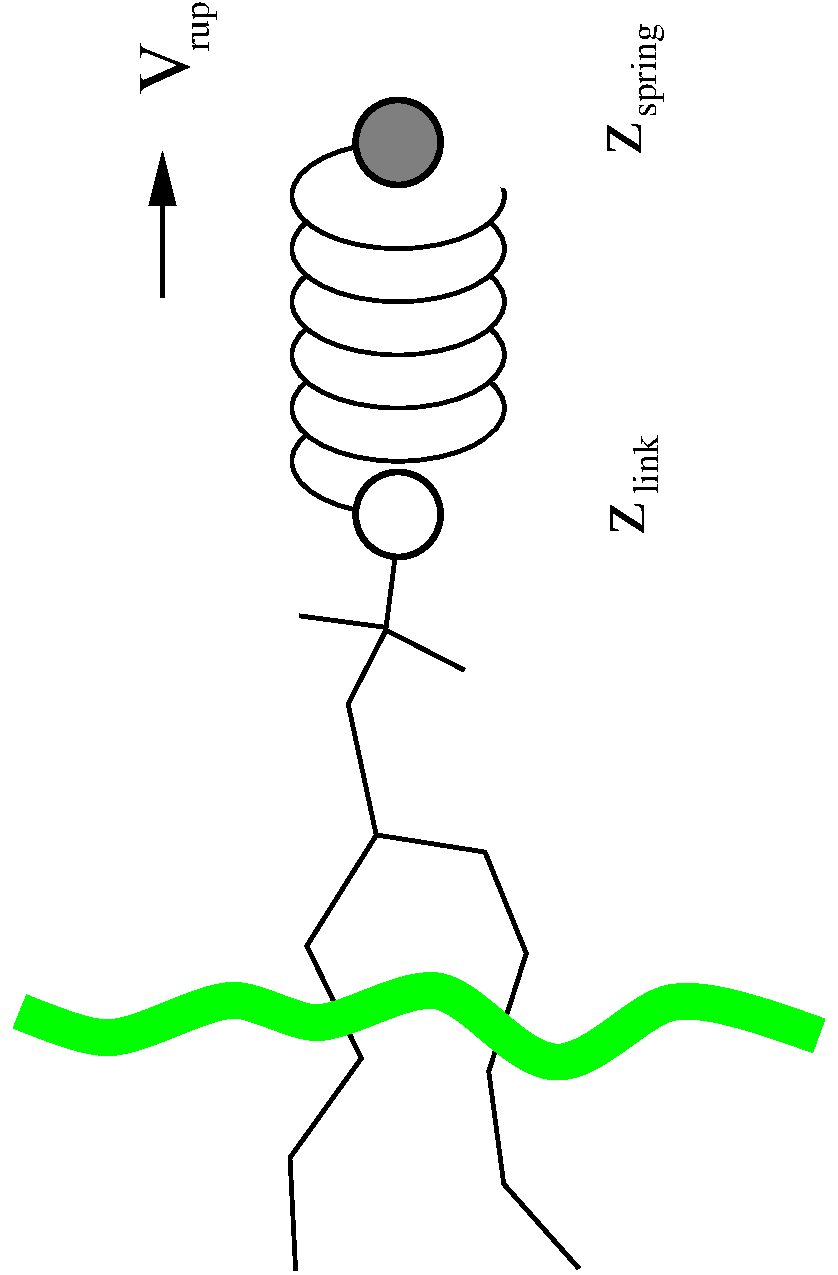
\includegraphics[width=6cm,angle=270]{plots/pull}}
\caption{Schematic picture of pulling a lipid out of a lipid bilayer
with umbrella pulling. $V_{rup}$ is the velocity at which the spring is
retracted, $Z_{link}$ is the atom to which the spring is attached and
$Z_{spring}$ is the location of the spring.}
\label{fi:pull} 
\end{figure}

Three different types of calculation are supported,
in all cases the reference distance can be constant
or linearly changing with time.
\begin{enumerate}
\item{\textbf{\swapindex{Umbrella}{pulling}}}
A harmonic potential is applied between
the centers of mass of two groups.
Thus the force is proportional to the displacement.
\item{\textbf{\swapindex{Constraint}{pulling}}}
The distance between the centers of mass of two groups is constrained.
The constraint force can be written to a file.
This method uses the SHAKE algorithm but only needs 1 iteration to be
exact if only two groups are constrained. 
\item{\textbf{Constant force pulling}}
A constant force is applied between the centers of mass of two groups.
Thus the potential is linear.
In this case there is no reference distance of pull rate.
\end{enumerate}

\subsubsection{Definition of the center of mass}

In {\gromacs} there are two ways to define the center of mass of a group.
The standard way is a ``plain'' center of mass, possibly with additional
weighting factors. With periodic boundary conditions it is no longer
possible to uniquely define the center of mass of a group of atoms.
Therefore a reference atom is used. For determining the center of mass,
for all other atoms in the group the periodic image is used which is
closed to the reference atom. This uniquely defines the center of mass.
By default the middle (determined by the order in the topology) atom
is used as a reference atom, but the user can also select any other atom,
if this would be closer to center of the group.

For a layered system, for instance a lipid bilayer, it may be of interest
to calculate the PMF of a lipid as function of its distance
from the whole bilayer. The whole bilayer can be taken as reference
group in that case, but it might also be of interest to define the
reaction coordinate for the PMF more locally. The {\tt mdp} option
{\tt pull\_geometry = cylinder} does not
use all the atoms of the reference group, but instead dynamically only those
within a cylinder with radius {\tt r\_1} around the pull vector going
through the pull group. This only
works for distances defined in one dimension, and the cylinder is
oriented with its long axis along this one dimension. A second cylinder
can be defined with {\tt r\_0}, with a linear switch function that weighs
the contribution of atoms between {\tt r\_0} and {\tt r\_1} with
distance. This smoothes the effects of atoms moving in and out of the
cylinder (which causes jumps in the pull forces).

\begin{figure}
\centerline{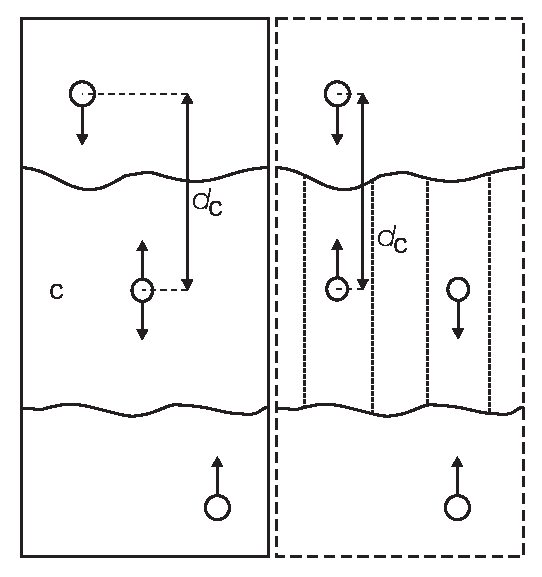
\includegraphics[width=6cm]{plots/pullref}}
\caption{Overview of the different reference group possibilities,
applied to interface systems. C is the reference group. The circles
represent the center of mass of two groups plus the reference group,
$d_c$ is the reference distance.}
\label{fi:pullref} 
\end{figure}   

When relative weights $w_i$ are used during the calculations, either
by supplying weights in the input or due to cylinder geometry,
the weights need to be scaled to conserve momentum:
\beq
w'_i = w_i
\left. \sum_{j=1}^N w_j \, m_j \right/ \sum_{j=1}^N w_j^2 \, m_j
\eeq
where $m_j$ is the mass of atom $j$ of the group.
The mass of the group, required for calculating the constraint force, is:
\beq
M = \sum_{i=1}^N w'_i \, m_i
\eeq
The definition of the weighted center of mass is:
\beq
\ve{r}_{com} = \left. \sum_{i=1}^N w'_i \, m_i \, \ve{r}_i \right/ M
\eeq
From the centers of mass the AFM, constraint or umbrella force $\ve{F}_{\!com}$
on each group can be calculated.
The force on the center of mass of a group is redistributed to the atoms
as follows:
\beq
\ve{F}_{\!i} = \frac{w'_i \, m_i}{M} \, \ve{F}_{\!com}
\eeq

\subsubsection{Limitations}
There is one important limitation:
strictly speaking, constraint forces can only be calculated between
groups that are not connected by constraints to the rest of the system.
If a group contains part of a molecule of which the bondlengths
are constrained, the pull constraint and LINCS or SHAKE bond constraint
algorithms should be iterated simultaneously. This is not done in {\gromacs}.
This means that for simulations with {\tt constraints = all-bonds}
in the {\tt .mdp} file pulling is, strictly speaking,
limited to whole molecules or groups of molecules.
In some cases this limitation can be avoided by using the free energy code,
see \secref{fepmf}.
In practice the errors caused by not iterating the two constraint
algorithms can be negligble when the pull group consists of a large
amount of atoms and/or the the pull force is small.
In such cases the constraint correction displacement of the pull group
is small compared to the bond lengths.


\section{Calculating a PMF using the free-energy code}
\label{sec:fepmf}
\index{potentials of mean force}
\index{free energy calculations}
The free-energy coupling-parameter approach (see \secref{fecalc})
provides several ways to calculate potentials of mean force.
A potential of mean force between two atoms can be calculated
by connecting them with a harmonic potential or a constraint
(for this purpose there a special potentials that avoid the generation of
extra exclusions, see \secref{excl}).
When the position of the minimum or the constraint length is 1 nm more
in state B than in state A, the restraint or constraint force is given
by $\partial H/\partial \lambda$.
The distance between the atoms can be changed as a function of $\lambda$
and time by setting {\tt delta-lambda} in the {\tt .mdp} file.
The results should be identical (although not numerically
due to the different implementations) to the results of the pull code
with umbrella sampling and constraint pulling.
Unlike the pull code, the free energy code can also handle atoms that
are connected by constraints.

Potentials of mean force can also be calculated using position restraints.
With position restraints atoms can be linked to a position in space
with a harmonic potential (see \secref{posre}).
These positions can be made a function of the coupling parameter $\lambda$.
The positions for the A and the B state are supplied to {\tt grompp} with
the {\tt -r} and {\tt -rb} option, respectively.
One could use this approach to do \normindex{targeted MD};
note that we do not encourage the use of targeted MD for proteins.
A protein can be forced from one conformation to another by using
these conformations as position restraint coordinates for state A and B.
One can then slowly change $\lambda$ from 0 to 1.
The main drawback of this approach is that the conformational freedom
of the protein is severely limited by the position restraints,
independent of the change from state A to B.
Also the protein is forced from state A to B in an almost straight line,
whereas the real pathway might be very different.
An example of a more fruitful application is a solid system or a liquid
confined between walls were one wants to measure the force required
to change the separation between the boundaries or walls.
Because the boundaries or walls already need to be fixed,
the position restraints do not limit the system in its sampling.

%%%%%%%%%%%%%%%%%%%%%%%%%%%%%%%%%%%%%%%%%%%%%%%%%%%%%%%%%%%%%%%%%%%%%%%%%%%%%%%
%%%%%%%%%%%%%%%%%%%%%%%%%%%%%%%%%%%%%%%%%%%%%%%%%%%%%%%%%%%%%%%%%%%%%%%%%%%%%%%
%%%%%%%%%%%%%%%%%%%%%%%%%%%%%%%%%%%%%%%%%%%%%%%%%%%%%%%%%%%%%%%%%%%%%%%%%%%%%%%
\newcommand{\amine}{\sf -NH$_2$}
\newcommand{\amines}{\sf -NH-}
\newcommand{\aminep}{\sf -NH$_3^+$}
\section{Removing fastest \swapindex{degrees of}{freedom}}
\label{sec:rmfast}
The maximum time step in MD simulations is limited by the smallest
oscillation period that can be found in the simulated
system. Bond-stretching vibrations are in their quantum-mechanical
ground state and are therefore better represented by a constraint than
by a harmonic potential.

For the remaining degrees of freedom, the shortest oscillation period
as measured from a simulation is 13~fs for bond-angle vibrations
involving hydrogen atoms. Taking as a guideline that with a Verlet
(leap-frog) integration scheme a minimum of 5 numerical integration
steps should be performed per period of a harmonic oscillation in
order to integrate it with reasonable accuracy, the maximum time step
will be about 3~fs. Disregarding these very fast oscillations of
period 13~fs the next shortest periods are around 20~fs, which will
allow a maximum time step of about 4~fs

Removing the bond-angle degrees of freedom from hydrogen atoms can
best be done by defining them as \normindex{virtual interaction-sites}
instead of normal atoms. Where a normal atoms is connected to the molecule
with bonds, angles and dihedrals, a virtual site's position is calculated
from the position of three nearby heavy atoms in a predefined manner
(see also \secref{virtual_sites}). For the hydrogens in water and in
hydroxyl, sulfhydryl or amine groups, no degrees of freedom can be
removed, because rotational freedom should be preserved. The only
other option available to slow down these motions, is to increase the
mass of the hydrogen atoms at the expense of the mass of the connected
heavy atom. This will increase the moment of inertia of the water
molecules and the hydroxyl, sulfhydryl or amine groups, without
affecting the equilibrium properties of the system and without
affecting the dynamical properties too much. These constructions will
shortly be described in \secref{vsitehydro} and have previously
been described in full detail~\cite{feenstra99}.

Using both virtual sites and \swapindex{modified}{mass}es, the next
bottleneck is likely to be formed by the improper dihedrals (which are
used to preserve planarity or chirality of molecular groups) and the
peptide dihedrals. The peptide dihedral cannot be changed without
affecting the physical behavior of the protein. The improper dihedrals
that preserve planarity, mostly deal with aromatic residues. Bonds,
angles and dihedrals in these residues can also be replaced with
somewhat elaborate virtual site constructions.

All modifications described in this section can be performed using the
{\gromacs} topology building tool {\tt \normindex{pdb2gmx}}. Separate
options exist to increase hydrogen masses, virtualize all hydrogen atoms
or also virtualize all aromatic residues. Note that when all hydrogen
atoms are virtualized, also those inside the aromatic residues will be
virtualized, {\ie} hydrogens in the aromatic residues are treated
differently depending on the treatment of the aromatic residues.

Parameters for the virtual site constructions for the hydrogen atoms are
inferred from the forcefield parameters ({\em vis}. bond lengths and
angles) directly by {\tt \normindex{grompp}} while processing the
topology file.  The constructions for the aromatic residues are based
on the bond lengths and angles for the geometry as described in the
forcefields, but these parameters are hard-coded into {\tt
\normindex{pdb2gmx}} due to the complex nature of the construction
needed for a whole aromatic group.

\subsection{Hydrogen bond-angle vibrations}
\label{sec:vsitehydro}
\subsubsection{Construction of virtual sites} %%%%%%%%%%%%%%%%%%%%%%%%%
\begin{figure}
\centerline{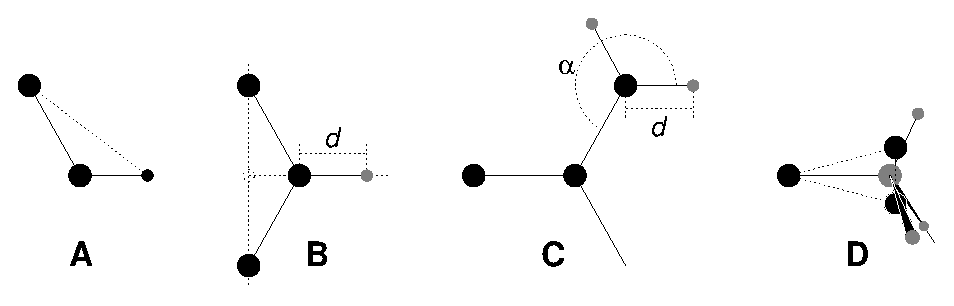
\includegraphics[width=11cm]{plots/dumtypes}}
\caption[Virtual site constructions for hydrogen atoms.]{The different
types of virtual site constructions used for hydrogen atoms. The atoms
used in the construction of the virtual site(s) are depicted as black
circles, virtual sites as grey ones. Hydrogens are smaller than heavy
atoms. {\sf A}: fixed bond angle, note that here the hydrogen is not a
virtual site; {\sf B}: in the plane of three atoms, with fixed distance;
{\sf C}: in the plane of three atoms, with fixed angle and distance;
{\sf D}: construction for amine groups ({\amine} or {\aminep}), see
text for details.}
\label{fig:vsitehydro}
\end{figure}

The goal of defining hydrogen atoms as virtual sites is to remove all
high-frequency degrees of freedom from them. In some cases not all
degrees of freedom of a hydrogen atom should be removed, {\eg} in the
case of hydroxyl or amine groups the rotational freedom of the
hydrogen atom(s) should be preserved. Care should be taken that no
unwanted correlations are introduced by the construction of virtual
sites, {\eg} bond-angle vibration between the constructing atoms could
translate into hydrogen bond-length vibration. Additionally, since
virtual sites are by definition massless, in order to preserve total
system mass, the mass of each hydrogen atom that is treated as virtual
site should be added to the bonded heavy atom.

Taking into account these considerations, the hydrogen atoms in a
protein naturally fall into several categories, each requiring a
different approach (see also \figref{vsitehydro}).

\begin{itemize}

\item{\em hydroxyl ({\sf -OH}) or sulfhydryl ({\sf -SH})
hydrogen:\/} The only internal degree of freedom in a hydroxyl group
that can be constrained is the bending of the {\sf C-O-H} angle. This
angle is fixed by defining an additional bond of appropriate length,
see \figref{vsitehydro}A. This removes the high frequency angle bending,
but leaves the dihedral rotational freedom. The same goes for a
sulfhydryl group. Note that in these cases the hydrogen is not treated
as a virtual site.

\item{\em single amine or amide ({\amines}) and aromatic hydrogens
({\sf -CH-}):\/} The position of these hydrogens cannot be constructed
from a linear combination of bond vectors, because of the flexibility
of the angle between the heavy atoms. Instead, the hydrogen atom is
positioned at a fixed distance from the bonded heavy atom on a line
going through the bonded heavy atom and a point on the line through
both second bonded atoms, see \figref{vsitehydro}B.

\item{\em planar amine ({\amine}) hydrogens:\/} The method used for
the single amide hydrogen is not well suited for planar amine groups,
because no suitable two heavy atoms can be found to define the
direction of the hydrogen atoms. Instead, the hydrogen is constructed
at a fixed distance from the nitrogen atom, with a fixed angle to the
carbon atom, in the plane defined by one of the other heavy atoms, see
\figref{vsitehydro}C.

\item{\em amine group (umbrella {\amine} or {\aminep}) hydrogens:\/}
Amine hydrogens with rotational freedom cannot be constructed as virtual
sites from the heavy atoms they are connected to, since this would
result in loss of the rotational freedom of the amine group. To
preserve the rotational freedom while removing the hydrogen bond-angle
degrees of freedom, two ``dummy masses'' are constructed with the same
total mass, moment of inertia (for rotation around the {\sf C-N} bond)
and center of mass as the amine group. These dummy masses have no
interaction with any other atom, except for the fact that they are
connected to the carbon and to each other, resulting in a rigid
triangle. From these three particles the positions of the nitrogen and
hydrogen atoms are constructed as linear combinations of the two
carbon-mass vectors and their outer product, resulting in an amine
group with rotational freedom intact, but without other internal
degrees of freedom. See \figref{vsitehydro}D.

\end{itemize}

\begin{figure}
\centerline{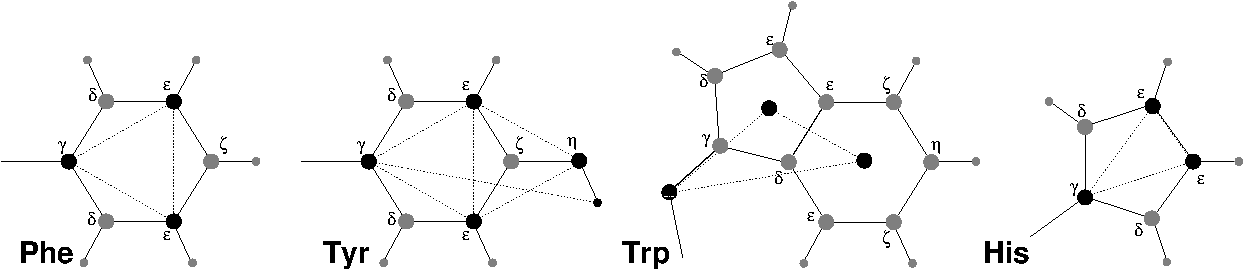
\includegraphics[width=15cm]{plots/dumaro}}
\caption[Virtual site constructions for aromatic residues.]{The
different types of virtual site constructions used for aromatic
residues. The atoms used in the construction of the virtual site(s) are
depicted as black circles, virtual sites as grey ones. Hydrogens are
smaller than heavy atoms. {\sf A}: phenylalanine; {\sf B}: tyrosine
(note that the hydroxyl hydrogen is {\em not} a virtual site); {\sf C}:
tryptophane; {\sf D}: histidine.}
\label{fig:vistearo}
\end{figure}

\subsection{Out-of-plane vibrations in aromatic groups}
\label{sec:vsitearo}
The planar arrangements in the side chains of the aromatic residues
lends itself perfectly to a virtual-site construction, giving a
perfectly planar group without the inherently instable constraints
that are necessary to keep normal atoms in a plane. The basic approach
is to define three atoms or dummy masses with constraints between them
to fix the geometry and create the rest of the atoms as simple virtual
sites type (see \secref{virtual_sites}) from these three. Each of
the aromatic residues require a different approach:

\begin{itemize}

\item{\em Phenylalanine:\/} {\sf C}$_\gamma$, {\sf C}$_{{\epsilon}1}$
and {\sf C}$_{{\epsilon}2}$ are kept as normal atoms, but with each a
mass of one third the total mass of the phenyl group. See
\figref{vsitehydro}A.

\item{\em Tyrosine:\/} The ring is treated identical to the
phenylalanine ring. Additionally, constraints are defined between {\sf
C}$_{{\epsilon}1}$ and {\sf C}$_{{\epsilon}2}$ and {\sf O}$_{\eta}$.
The original improper dihedral angles will keep both triangles (one
for the ring and one with {\sf O}$_{\eta}$) in a plane, but due to the
larger moments of inertia this construction will be much more
stable. The bond angle in the hydroxyl group will be constrained by a
constraint between {\sf C}$_\gamma$ and {\sf H}$_{\eta}$, note that
the hydrogen is not treated as a virtual site. See
\figref{vsitehydro}B.

\item{\em Tryptophane:\/} {\sf C}$_\beta$ is kept as a normal atom
and two dummy masses are created at the center of mass of each of the
rings, each with a mass equal to the total mass of the respective ring
({\sf C}$_{{\delta}2}$ and {\sf C}$_{{\epsilon}2}$ are each
counted half for each ring). This keeps the overall center of mass and
the moment of inertia almost (but not quite) equal to what it was. See
\figref{vsitehydro}C.

\item{\em Histidine:\/} {\sf C}$_\gamma$, {\sf C}$_{{\epsilon}1}$
and {\sf N}$_{{\epsilon}2}$ are kept as normal atoms, but with masses
redistributed such that the center of mass of the ring is
preserved. See \figref{vsitehydro}D.

\end{itemize}

\section{\normindex{Viscosity} calculation}

The shear viscosity is a property of liquid which can be determined easily  
by experiment. It is useful for parameterizing the forcefield,
because it is a kinetic property, while most other properties
which are used for parameterization are thermodynamic.
The viscosity is also an important property, since it influences
the rates of conformational changes of molecules solvated in the liquid.

The viscosity can be calculated from an equilibrium simulation using
an Einstein relation:
\beq
\eta = \frac{1}{2}\frac{V}{k_B T} \lim_{t \rightarrow \infty}
\frac{\mbox{d}}{\mbox{d} t} \left\langle 
\left( \int_{t_0}^{{t_0}+t} P_{xz}(t') \mbox{d} t' \right)^2
\right\rangle_{t_0}
\eeq
This can be done with {\tt g\_energy}.
This method converges very slowly~\cite{Hess2002a}.
A nanosecond simulation might not
be long enough for an accurate determinination of the viscoity.
The result is very dependent on the treatment of the electrostatics.
Using a (short) cut-off results in large noise on the off-diagonal
pressure elements, which can increase the calculated viscosity by an order
of magnitude.

{\gromacs} also has a non-equilibrium method for determining
the viscosity~\cite{Hess2002a}.
This makes use of the fact that energy, which is fed into system by
external forces, is dissipated through viscous friction. The generated heat
is removed by coupling to a heat bath. For a Newtonian liquid adding a 
small force will result in a velocity gradient according to the following
equation:
\beq
a_x(z) + \frac{\eta}{\rho} \frac{\partial^2 v_x(z)}{\partial z^2} = 0
\eeq
here we have applied an acceleration $a_x(z)$ in the $x$-direction, which
is a function of the $z$-coordinate.
In {\gromacs} the acceleration profile is:
\beq
a_x(z) = A \cos\left(\frac{2\pi z}{l_z}\right)
\eeq
where $l_z$ is the height of the box. The generated velocity profile is:
\beq
v_x(z) = V \cos\left(\frac{2\pi z}{l_z}\right)
\eeq
\beq
V = A \frac{\rho}{\eta}\left(\frac{l_z}{2\pi}\right)^2
\eeq
The viscosity can be calculated from $A$ and $V$:
\beq
\label{visc}
\eta = \frac{A}{V}\rho \left(\frac{l_z}{2\pi}\right)^2
\eeq

In the simulation $V$ is defined as:
\beq
V = \frac{\displaystyle \sum_{i=1}^N m_i v_{i,x} 2 \cos\left(\frac{2\pi z}{l_z}\right)}
         {\displaystyle \sum_{i=1}^N m_i}
\eeq
The generated velocity profile is not coupled to the heat bath, moreover
the velocity profile is excluded from the kinetic energy.
One would like $V$ to be as large as possible to get good statistics.
However the shear rate should not be so high that the system gets too far
from equilibrium. The maximum shear rate occurs where the cosine is zero,
the rate being:
\beq
\mbox{sh}_{\max} =  \max_z \left| \frac{\partial v_x(z)}{\partial z} \right|
= A \frac{\rho}{\eta} \frac{l_z}{2\pi}
\eeq
For a simulation with: $\eta=10^{-3}$ [kg\,m$^{-1}$\,s$^{-1}$],
$\rho=10^3$\,[kg\,m$^{-3}$] and $l_z=2\pi$\,[nm],
$\mbox{sh}_{\max}=1$\,[ps\,nm$^{-1}$] $A$.
This shear rate should be smaller than one over the longest
correlation time in the system. For most liquids this will be the rotation
correlation time, which is around 10 picoseconds. In this case $A$ should
be smaller than 0.1\,[nm\,ps$^{-2}$].
When the shear rate is too high, the observed viscosity will be too low.
Because $V$ is proportional to the square of the box height,
the optimal box is elongated in the $z$-direction.
In general a simulation length of 100 picoseconds is enough to obtain an
accurate value for the viscosity.

The heat generated by the viscous friction is removed by coupling to a heat
bath. Because this coupling is not instantaneous the real temperature of the
liquid will be slightly lower than the observed temperature.
Berendsen derived this temperature shift\cite{Berendsen91}{,} which can
be written in terms of the shear rate as:
\beq
T_s = \frac{\eta\,\tau}{2 \rho\,C_v} \mbox{sh}_{\max}^2
\eeq
where $\tau$ is the coupling time for the Berendsen thermostat and
$C_v$ is the heat capacity. Using the values of the example above,
$\tau=10^{-13}$ [s] and $C_v=2 \cdot 10^3$\,[J kg$^{-1}$\,K$^{-1}$], we
get: $T_s=25$\,[K\,ps$^{-2}$]\,sh$_{\max}^2$. When we want the shear
rate to be smaller than $1/10$\,[ps$^{-1}$], $T_s$ is smaller than
0.25\,[K], which is negligible.

Note that the system has to build up the velocity profile when starting
from an equilibrium state. This build-up time is of the order of the
correlation time of the liquid.

Two quantities are written to the energy file, along with their averages
and fluctuations: $V$ and $1/\eta$ as obtained from (\ref{visc}).

\section{\normindex{Tabulated interaction function}s}
\subsection{Cubic splines for potentials}
\label{subsec:cubicspline}
In some of the inner loops of {\gromacs} lookup tables are used 
for computation of potential and forces. 
The tables are interpolated using a cubic
spline algorithm. 
There are separate tables for electrostatic, dispersion and repulsion
interactions,
but for the sake of caching performance these have been combined
into a single array. 
The cubic spline interpolation for $x_i \leq x < x_{i+1}$ looks like this:
\beq
V_s(x) = A_0 + A_1 \,\epsilon + A_2 \,\epsilon^2 + A_3 \,\epsilon^3
\label{eqn:spline}
\eeq
where the table spacing $h$ and fraction $\epsilon$ are given by:
\bea
h	&=&	x_{i+1} - x_i	\\
\epsilon&=&	(x - x_i)/h
\eea
so that $0 \le \epsilon < 1$.
From this we can calculate the derivative in order to determine the forces:
\beq
-V_s'(x) ~=~ 
-\frac{{\rm d}V_s(x)}{{\rm d}\epsilon}\frac{{\rm d}\epsilon}{{\rm d}x} ~=~
-(A_1 + 2 A_2 \,\epsilon + 3 A_3 \,\epsilon^2)/h
\eeq
The four coefficients are determined from the four conditions
that $V_s$ and $-V_s'$ at both ends of each interval should match
the exact potential $V$ and force $-V'$.
This results in the following errors for each interval:
\bea
|V_s  - V  |_{max} &=& V'''' \frac{h^4}{384} + O(h^5) \\
|V_s' - V' |_{max} &=& V'''' \frac{h^3}{72\sqrt{3}} + O(h^4) \\
|V_s''- V''|_{max} &=& V'''' \frac{h^2}{12}  + O(h^3)
\eea
V and V' are continuous, while V'' is the first discontinuous
derivative.
The number of points per nanometer is 500 and 2000
for single and double precision compiled versions of {\gromacs}, respectively.
This means that the errors in the potential and force will usually
be smaller than the single precision accuracy.

{\gromacs} stores $A_0$, $A_1$, $A_2$ and $A_3$.
The force routines get a table with these four parameters and
a scaling factor $s$ that is equal to the number of points per nm.
(Note that $h$ is $s^{-1}$).
The algorithm goes a little something like this:
\begin{enumerate}
\item	Calculate distance vector (\ve{r}$_{ij}$) and distance r$_{ij}$
\item	Multiply r$_{ij}$ by $s$ and truncate to an integer value $n_0$
	to get a table index
\item	Calculate fractional component ($\epsilon$ = $s$r$_{ij} - n_0$) 
	and $\epsilon^2$ 
\item	Do the interpolation to calculate the potential $V$ and the the scalar force $f$
\item	Calculate the vector force \ve{F} by multiplying $f$ with \ve{r}$_{ij}$
\end{enumerate}

Note that table lookup is significantly {\em
slower} than computation of the most simple Lennard-Jones and Coulomb
interaction. However, it is much faster than the shifted coulomb
function used in conjunction with the PPPM method. Finally it is much
easier to modify a table for the potential (and get a graphical
representation of it) than to modify the inner loops of the MD
program.

\subsection{User specified potential functions}
You can also use your own \swapindex{potential}{function}s 
without editing the {\gromacs} code. 
The potential function should be according to the following equation
\beq
V(r_{ij}) ~=~ \frac{q_i q_j}{4 \pi\epsilon_0} f(r_{ij}) + C_6 \,g(r_{ij}) + C_{12} \,h(r_{ij})
\eeq
with f,g,h user defined functions. Note that if g(r) represents a
normal dispersion interaction, g(r) should be $<$ 0. C$_6$, C$_{12}$
and the charges are read from the topology. Also note that combination
rules are only supported for Lennard Jones and Buckingham, and that
your tables should match the parameters in the binary topology.

When you add the following lines in your {\tt .mdp} file:\\
\begin{tt}
rlist           = 1.0\\
coulombtype     = User\\
rcoulomb        = 1.0\\
vdwtype         = User\\
rvdw            = 1.0\\
\end{tt}
the MD program will read a single non-bonded table file,
or multiple when {\tt energygrp\_table} is set (see below).
The name of the file(s) can be set with the mdrun option {\tt -table}.
The table file should contain seven columns of table lookup data in the
order: $x$, $f(x)$, $-f'(x)$, $g(x)$, $-g'(x)$, $h(x)$, $-h'(x)$.
The $x$ should run from 0 to $r_c+1$ (the value table extension can be
changed in the {\tt .mdp} file).
You can choose the spacing you like; for the standard tables {\gromacs}
uses a spacing of 0.002 and 0.0005 nm when you run in single
and double precision, respectively.  In this
context $r_c$ denotes the maximum of the two cut-offs {\tt rvdw} and
{\tt rcoulomb} (see above). These variables need not be the same (and
need not be 1.0 either).  Some functions used for potentials contain a
singularity at x = 0, but since atoms are normally not closer to each
other than 0.1 nm, the function value at x = 0 is not important.
Finally, it is also
possible to combine a standard Coulomb with a modified LJ potential
(or vice versa). One then specifies e.g. coulombtype = Cut-off or
coulombtype = PME, combined with vdwtype = User.  The table file must
always contain the 7 columns however, and meaningful data (i.e. not
zeroes) must be entered in all columns.  A number of pre-built table
files can be found in the GMXLIB directory, for 6-8, 6-9, 6-10, 6-11, 6-12
Lennard Jones potentials combined with a normal Coulomb.

If you want to have different functional forms between different
groups of atoms, this can be set through energy groups.
Different tables can be used for non-bonded interactions between
different energy groups pairs through the mdp option {\tt energygrp\_table}
(see \secref{mdpopt}).
Atoms that should interact with a different potential should
be put into different energy groups.
Between group pairs which are not listed in {\tt energygrp\_table},
the normal user tables will be used. This makes it easy to use
a different functional form between a few types of atoms.

\section{Mixed Quantum-Classical simulation techniques}

In a molecular mechanics (MM) forcefield, the influence of electrons
is expressed by empirical parameters that are assigned on the basis of
experimental data, or on the basis of results from high-level quantum
chemistry calculations. These are valid for the ground state of a
given covalent structure, and the MM approximation is usually
sufficiently accurate for ground-state processes in which the overall
connectivity between the atoms is the system remains
unchanged. However, for processes in which the connectivity does
change, such as chemical reactions, or processes that involve multiple
electronic states, such as photochemical conversions, electrons can no
longer be ignored, and a quantum mechanical description is required
for at least those parts of the system in which the reaction takes
place.

One approach to the simulation of chemical reactions in solution, or
in enzymes, is to use a combination of quantum mechanics (QM) adn
molecular mechanics (MM). The reacting parts of the system are treated
quantum mechanically, with the remainder being modelled using the
forcefield. The current version of Gromacs provides interfaces to
several popular Quantum Chemistry packages (Mopac\cite{mopac},
Gamess-UK\cite{gamess-uk}, Gaussian\cite{g03} and CPMD\cite{Car85a}).

Gromacs interactions between the two subsystems are
either handled as described by Field {\it{et al.}}\cite{Field90a} or
within the ONIOM approach by Morokuma and coworkers\cite{Maseras96a,
Svensson96a}.

\subsection{Overview}

Two approaches for describing the interactions between the QM and MM
subsystems are supported in this version:

\begin{enumerate}
\item{\textbf{Electronic Embedding}} The electrostatic interactions
between the electrons of the QM region and the MM atoms and between
the QM nuclie and the MM atoms, are included in the Hamiltonian for
the QM subsystem: \beq H^{QM/MM} =
H^{QM}_e-\sum_i^n\sum_J^M\frac{e^2Q_J}{4\pi\epsilon_0r_{iJ}}+\sum_A^N\sum_J^M\frac{e^2Z_AQ_J}{e\pi\epsilon_0R_{AJ}},
\eeq where $n$ and $N$ are the number of electrons and nuclei in the
QM region, respectively, and $M$ is the number of charged MM
atoms. The first term on the right hand side is the original
electronic Hamiltonian of an isolated QM system. The first of the
double sums us the total electrostatic interaction between the QM
electrons and the MM atoms. The total electrostatic interaction of the
QM nuclei with the MM atoms is given by the second double sum. Bonded
interactions between QM and MM atoms are described at the MM level by
the appropriate forcefield terms. Chemical bonds that connect the two
subsystems are capped by a hydrogen atom to complete the valence of
the QM region. The force on this atom, which is present in the QM
region only, is distributed over the two atoms of the bond. The cap
atom is usually referred to as a link atom.

\item{\textbf{ONIOM}} In the ONIOM approach, the energy and gradients
are first evaluated for the isolated QM subsystem at the desired level
of {\it{ab initio}} theory. Subsequently, the energy and gradients of
the total system, including the QM region, are computed using the
molecular mechanics forcefield and added to the energy and gradients
calculated for the isolated QM subsystem. Finally in order to correct
for counting the interactions inside the QM region twice, a molecular
mechanics calculation is performed on the isolated QM subsystem and
the energy and gradients are subtracted. This leads to the following
expression for the total QM/MM energy (and gradients likewise): \beq
E_{tot} = E_{I}^{QM}
+E_{I+II}^{MM}-E_{I}^{MM}, \eeq where the
subscripts I and II refer to the QM and MM subsystems,
respectively. The superscripts indicate at what level of theory the
energies are computed. The ONIOM scheme has the advantage has the
advantage that it is not restricted to a two layer QM/MM description,
but can easily handle more than two layers, with each layer described
at a different level of theory.
\end{enumerate}

\subsection{Usage}

To make use of the QM/MM functionality in Gromacs, one needs to:

\begin{enumerate}
\item introduce link atoms at the QM/MM boundary, if needed;
\item specify which atoms are to be treated at a QM level;
\item specify the QM level, basisset, type of QM/MM interface and so on. 
\end{enumerate}

\subsubsection{Adding link atoms}

At the bond that connects the QM and MM subsystems a link atoms is
introduced.  In Gromacs the link atom has special atomtype, called
LA. This atomtype is treated as a hydrogen atom in the QM calculation,
and as a dummy atom in the forcefield calculation. The link atoms, if
any, are part of the system, but have no interaction with any other
atom, except that the QM force working on it is distributed over the
two atoms of the bond. In the topology the link atom (LA), therefore,
is defined as a virtual site atom:\\

\begin{tt}
[ virtual\_sites2 ]\\
LA QMatom MMatom 1 0.65\\
\end{tt}

See the dummy atoms section for more details on how dummies are
treated. The link atom is replaced at every step of the simulation.

In addition, the bond itself is replaced by a constraint:

\begin{tt}
[ constraints ] \\
QMatom MMatom 2 0.153\\
\end{tt}

Note that, because in our system the QM/MM bond is a carbon-carbon
bond (0.153 nm), we use a constraint length of 0.153 nm, and dummy
position of 0.65. The latter is the ratio between the ideal C-H
bondlength and the ideal C-C bond length. With this ratio, the link
atom is always 0.1 nm away from the QMatom, consistent with the
carbon-hydrogen bondlength. If the QM and MM subsystems are connected
by a different kind of bond, a different constraint and a different
dummy position, appropriate for that bond type, are required.

\subsubsection{Specifying the QM atoms}

Atoms that should be treated at a QM level of theory, including the
link atoms, are added to the index file. In addition, the chemical
bonds between the atoms in the QM region are to be defined as
connect bonds (bond type 5)in the topology file:

\begin{tt}
[ bonds ]\\
QMatom1 QMatom2 5\\
QMatom2 QMatom3 5\\
\end{tt}

\subsubsection{Specifying the QM/MM simulation parameters}

In the mdp file, the following parameters control a QM/MM simulation.

\begin{description}

\item[\tt QMMM = no]\mbox{}\\ If this is set to {\tt yes}, a QM/MM
simulation is requested. Several groups of atoms can be described at
different QM levels separately. These are specified in the QMMM-grps
field separated by spaces. The level of {\it{ab initio}} theory at which the
groups are described is speficied by {\tt QMmethod} and {\tt QMbasis}
Fields. Describing the groups at different levels of theory is only
possible with the ONIOM QM/MM scheme, specified by {\tt QMMMscheme}.

\item[\tt QMMM-grps =]\mbox{}\\groups to be descibed at the QM level

\item[\tt QMMMscheme = normal]\mbox{}\\Options are {\tt normal} and
{\tt ONIOM}. This selects the QM/MM interface. {\tt normal} implies
that the QM subsystem is electronically embedded in the MM
subsystem. There can only be one {\tt QMMM-grps} that is modelled at
the {\tt QMmethod} and {\tt QMbasis} level of {\it{ ab initio}}
theory. The rest of the system is described at the MM level. The QM
and MM subsystems interact as follows: MM point charges are included
in the QM one-electron hamiltonian and all Lennard-Jones interactions
are described at the MM level. If {\tt ONIOM} is selected, the
interaction between the subsystem is described using the ONIOM method
by Morokuma and co-workers. There can be more than one QMMM-grps each
modelled at a different level of QM theory (QMmethod and QMbasis).

\item[\tt QMmethod = ]\mbox{}\\Method used to compute the energy
and gradients on the QM atoms. Available methods are AM1, PM3, RHF,
UHF, DFT, B3LYP, MP2, CASSCF, MMVB and CPMD. For CASSCF, the number of
electrons and orbitals included in the active space is specified by
{\tt CASelectrons} and {\tt CASorbitals}. For CPMD, the planewave
cut-off is specified by the {\tt planewavecutoff} keyword.

\item[\tt QMbasis = ]\mbox{}\\Gaussian basisset used to expand the
electronic wavefuntion. Only gaussian bassisets are currently
available, i.e. STO-3G, 3-21G, 3-21G*, 3-21+G*, 6-21G, 6-31G, 6-31G*,
6-31+G*, and 6-311G. For CPMD, whcih uses plane wave expansion rather
than atom-centered basisfunctions, the {\tt planewavecutoff} keyword
controls the plane wave expansion.

\item[\tt QMcharge = ]\mbox{}\\The total charge in {\it{e}} of the {\tt
QMMM-grps}. In case there are more than one {\tt QMMM-grps}, the total
charge of each ONIOM layer needs to be specified separately.

\item[\tt QMmult = ]\mbox{}\\The multiplicity of the {\tt
QMMM-grps}. In case there are more than one {\tt QMMM-grps}, the
multiplicity of each ONIOM layer needs to be specified separately.

\item[\tt CASorbitals = ]\mbox{}\\The number of orbitals to be
included in the active space when doing a CASSCF computation.

\item[\tt CASelectrons = ]\mbox{}\\The number of electrons to be
included in the active space when doing a CASSCF computation.

\item[\tt SH = no]\mbox{}\\If this is set to yes, a QM/MM MD
simulation on the excited state-potential energy surface and enforce a
diabatic hop to the ground-state when the system hits the conical
intersection hyperline in the course the simulation. This option only
works in combination with the CASSCF method.

\end{description}

\subsection{Output}

The energies and gradients computed in the QM calculation are added to
those computed by gromacs. In the {\tt .edr} file there is a section
for the total QM energy.

\subsection{Future developments}

Several features are currently under development that increase the
accuracy of the QM/MM interface. One useful feature is the use of
delocalized MM charges in the QM computations. The most important
benefit of using such smeared-out charges is that the coulombic
potential has a finite value at inter atomic distances. In the point
charge representation, the partially charged MM atoms close to the QM
region, tend to 'overpolarize' the QM system, which leads to artefacts
in the calculation.

What is needed as well is a transition state optimizer.

\section{Gromacs on GPUs}

This is an experimental release of {\gromacs} for accelerated
Molecular Dynamics simulations on GPU accelerators. Support is provided
by the \href{https://simtk.org/home/openmm}{OpenMM library}. This release is
targeted at developers and advanced users and care should be taken before production use.
The following should be noted before using the GPU accelerated program:
\begin{itemize}
\item The current release runs only on modern NVIDIA GPU hardware with CUDA support.
Make sure that the necessary CUDA drivers and libraries for your operating system
are already installed. 
\item Multiple GPUs are not supported.
\item Only a fairly small subset of the {\gromacs} features and options are supported on the GPUs.
See below for a detailed list.
\item Consumer level GPU cards are known to often have problems with faulty memory.
It is recommended that a full memory check of the cards is done at least once
(for example, using the {\tt memtest=full} option).
A partial memory check (for example, {\tt memtest=15}) before and
after the simulation run would help spot
problems resulting from overheating of the graphics card.
\item The maximum size of the simulated systems depends on the available
GPU memory, for example, a GTX280 with 1GB memory has been tested with systems
of up to about 100,000 atoms.
\item In order to take a full advantage of the GPU platform features, many algorithms
have been implemented in a very different way than they are on the CPUs.
Therefore numercal correspondence between some properties of the systems' state
should not be expected. Moreover, the values will likely vary when simulations are
done on different GPU hardware. However, sufficiently long trajectories
should produce comparable statistical averages.
\item Frequent retrieval of system state information such as
trajectory coordinates and energies can greatly influence the performance
of the program due to slow CPU$<$--$>$GPU memory transfer speed.
\item MD algorithms are complex, and although the Gromacs code is highly tuned for them,
they often do not translate very well onto the streaming architetures.
Realistic expectations about the achievable speed-up from tests with GTX280:
for small protein systems in implicit solvent using all-vs-all kernels the acceleration
can be as high as 20 times, but in most other setups involving cutoffs and PME the
acceleration is usually only 4~6 times relative to a 3GHz CPU. ?????
\end{itemize}

\subsection{Supported features}

\begin{itemize}
\item \textbf{Integrators:} {\tt md/md-vv/md-vv-avek}, {\tt sd/sd1} and {\tt bd}.\\
OpenMM implements only the velocity-verlet algorithm for MD simulations.
Option {\tt md} is accepted but keep in mind that the actual algorithm is not leap-frog.
Thus all three options {\tt md}, {\tt md-vv} and {\tt md-vv-avek} are equivalent.
Similarly, options {\tt sd} and {\tt sd1} are also equivalent.
\item \textbf{Long-range interactions:} {\tt Reaction-Field}, {\tt Ewald}, {\tt PME}.\\
{\tt No-cutoff}, i.e. {\tt rcoulomb=0} and {\tt rvdw=0}, is also supported.\\
For Ewald summation only 3D geometry is supported, and dipole correction is not.
\item \textbf{Temperature control:} Supported only with the {\tt sd/sd1}, {\tt bd},
{\tt md/md-vv/md-vv-avek} integrators.\\
OpenMM implements only the Andersen thermostat. All values for {\tt tcoupl} are
thus accepted and equivalent to {\tt andersen}. Multiple temperature coupling groups
are not supported, only {\tt tc-grps=System} will work. Remember that for heterogenous
systems such as membrane proteins, coupling of the whole system will likely lead to
different temperatures in the different phases - hot solvent and cold solute.
\item \textbf{Force fields:} Amber, ??? (not GROMOS!).
\item \textbf{Implicit solvent:} Supported only with {\tt reaction-field} electrostatics.
\item \textbf{Constraints:} Constraints in OpenMM are done by a combination of SHAKE,
SETTLE and CCMA. Accuracy is based on the SHAKE tolerance as set by the {\tt shake\_tol} option.
\item \textbf{Periodic Boundary Conditions:} Only {\tt pbc=xyz} and {\tt pbc=no} in rectangular cells(boxes) are supported.
\item \textbf{Pressure control:} Not supported.
\item \textbf{Simulated annealing:} Not supported.
\item \textbf{Pulling:} Not supported. 
\item \textbf{Restraints:} Distant, orientational, angle and dihedral restraints are not supported.
\item \textbf{Free energy calculations:} Not supported.
\item \textbf{Walls:} Not supported.
\item \textbf{Non-equilibrium MD:} Option {\tt acc\_grps} is not supported.
\item \textbf{Electric Fields:} Not supported.
\item \textbf{QMMM:} Not supported.
\end{itemize}

\subsection{Installing and running {\gromacs}-GPU}

{\gromacs}-GPU can be installed either from the officially distributed 
binary or source packages. 
We provide precompiled binaries built for and tested on the most common Linux, Windows, 
and Mac OS operating systems (for details see the {\gromacs}-GPU 
\href{???}{download page}). 
Using the binary distribution is highly recommended and it should 
work in most of the cases. Binary (as well as source) distributions are available 
for various platforms available on the Gromacs website. 
Below we summarize how to get the GPU accelerated mdrun-gpu work.

\subsubsection{Prerequisites}

The current {\gromacs}-GPU release uses \href{https://simtk.org/home/openmm}{OpenMM} 
acceleration, the necessary libraries and plugins are included in the binary 
packages (version svn r2234). 

Both the OpenMM library and {\gromacs}-GPU require version 3.0 of
the CUDA libraries and compatible NVIDIA driver. 

Last but not least, to run GPU accelerated simulations, a CUDA-enabled 
graphics card is necessary. Molecular dynamics algorithms 
are very demanding and unlike in other application areas, 
only high-end graphics cards are capable of providing performance comparable 
to/higher then modern CPUs. For this reason, mdrun-gpu is compatible with 
only a subset of CUDA-enabled GPUs (for detailed list see section 
\ref{subsec-compatibility}) and by default it does no run if detects 
non-compatible hardware. 

For details about compatibility of NVIDIA drivers with CUDA library and devices consult  
the \href{http://developer.nvidia.com/object/gpucomputing.html}{NVIDIA developer page}.

Summary of prerequisites: 
\begin{itemize}
    \item OpenMM;
    \item NVIDIA CUDA libraries;
    \item NVIDIA driver;
    \item NVIDIA CUDA-enabled GPU.
\end{itemize}


\subsubsection{Installing}

\begin{enumerate}

    \item Download and unpack the binary package for the respective OS and architecture. 
    Copy the content of the package to your normal Gromacs installation directory (or to a custom location).
    
    Note that as the distributed {\gromacs}-GPU packages do not contain the entire set of 
    tools and utilities included in a full Gromacs installation. Therefor, it is recommended to 
    have a $\geq$v4.0.7 ??? (is grompp-4.0.7 compatible with mdrun-4.5) ???
    standard Gromacs installation along the GPU accelerated one.

    \item Add the \footnotesize{\tt openmm/lib} directory to your library path,  e.g. in bash:\\
    \footnotesize{\tt export LD\_LIBRARARY\_PATH=path\_to\_gromacs/openmm/lib:\$LS\_LIBRARY\_PATH}.\\
    If there are other OpenMM versions installed, make sure that the supplied libraries have preference  
    when running mdrun-gpu. Also, make sure that the CUDA libraries installed match the version 
    of CUDA {\gromacs}-GPU is compiled with.

    \item Set the \footnotesize{\tt OPENMM\_LIBRARY\_PATH} environment variable to contain the path to 
    the \footnotesize{\tt openmm/lib/plugins} directory, e.g. in bash:\\ 
    \footnotesize{\tt export OPENMM\_LIBRARY\_PATH=path\_to\_gromacs/openmm/lib/plugins}.\\

    \item At this point, running the command
    \footnotesize{\tt path\_to\_gromacs/bin/mdrun-gpu -h} should display the standard mdrun help  
    which means that the binary runs and all the necessary libraries are accessible. 

\end{enumerate}

\subsubsection{Compiling mdrun-gpu}

The GPU accelerated mdrun can be compiled on Linux, Mac OS and Windows 
operating systems, both for 32 and 64 bit. Besides the prerequisites 
discussed above, in order to compile mdrun-gpu the following additional 
software is required: 
\begin{itemize}
    \item Cmake version $\leq$2.6.4
    \item CUDA-compatible compiler: 
        \begin{itemize}
            \item MSVC 8 or 9 on Windows 
            \item gcc 4.1--4.3 on Linux and Mac OS
        \end{itemize}
    \item OpenMM header files ( $\leq$svn r2234)
\end{itemize}
Note, that the current {\gromacs}-GPU release is compatible with OpenMM  
versions 1.1 and 1.1.1, but runs only on on pre-GF100 hardware. 
While future versions might be compatible, using the officially supported 
and tested OpenMM versions is strongly encouraged.
OpenMM binaries as well as source code can be obtained from the 
\href{https://simtk.org/project/xml/downloads.xml?group_id=161}{project homepage}.

Also note that compiling gromacs-gpu is possible using both CUDA 2.3 and 3.0,
however it is essential that the version of CUDA mdrun-gpu is compiled against 
matches the one used for compiling the OpenMM libraries. 

To compile mdrun-gpu change the directory top level of the source 
tree and execute the following commands: 
\begin{itemize}
    \item \footnotesize{\tt cmake  -DGMX\_OPENMM=ON [-DCMAKE\_INSTALL\_PREFIX=desired\_install\_path]}
    \item \footnotesize{\tt make mdrun}
    \item \footnotesize{\tt make install-mdrun} ???
\end{itemize}


\subsubsection{Testing and troubleshooting}

\subsubsection{{\gromacs}-GPU specific mdrun features}

Besides the usual command line options the mdrun tool supports, 
mdrun-gpu also supports a set of ``device options'', that are meant to 
give control over acceleration related functionalities. 
These options can be used in the following form:\\
\footnotesize{\tt mdrun-gpu -device "ACCELERATION:[DEV\_OPTION=VALUE,]... [OPTION].."}.\\

The option-list prefix \footnotesize{\tt ACCELERATION} specifies which 
acceleration library should be used. At the moment, the only supported value 
is \footnotesize{\tt OpenMM}. This is followed by the list of comma-separated
\footnotesize{\tt DEV\_OPTION=VALUE} option-value pairs which define 
parameters for the selected acceleration platform. the entire device option 
string is case insensitive.

Below we summarize the available options (of the OpenMM acceleration library)
and their possible values.

\paragraph{Platform} Selects the GPGPU platform to be used, currently the only 
supported value is CUDA (in future OpenCL support will be added).

\paragraph{DeviceID} The numeric identifier of the CUDA device on which the 
simulation will be carried out. The default value is 0, the first device. 

\paragraph{Memtest} GPUs, especially consumer-level devices, 
are prone to memory errors. There might be various reasons for 
''soft errors`` to happen including (factory) overclocking, overheating, 
faulty hardware etc, but the result is always the same: unreliable, possibly 
incorrect results. Therefor, gromacs-gpu has a built-in mechanism for 
testing the GPU memory in order to catch the obviously faulty hardware. 
A set of tests are performed before and after each simulation and if
errors are detected, the execution is aborted. 

Accepted values for this option are any integer $\leq$15 with an optional ``s'' 
prefix representing the approximate amount of time in seconds that should be spent 
on testing, the default value is \footnotesize{\tt memtest=15s}. 
It is possible to completely turn of memory testing by setting 
\footnotesize{\tt memtest=15s}, however this is not advisable.

\paragraph{Force-device} Option that enables running mdrun-gpu 
devices that are not supported but CUDA-capable. Using 
this option might results in very low performance or even 
crashes and therefor it is neither encouraged.

\subsection{Hardware and software compatibility list}\label{subsec-compatiblity}

Compatible OpenMM versions:
\begin{itemize}
\item up to svn r2234 (\textit{not} compatible with CUDA 2.3)
\item v1.1.1 (\textit{not} compatible with GF100)
\item v1.1 (\textit{not} compatible with GF100)
\end{itemize}

Compatible NVIDIA CUDA versions (also see OpenMM version compatibility above): 
\begin{itemize}
\item v2.3
\item v3.0
\end{itemize}

Compatible hardware (for details consult the 
\href{http://www.nvidia.com/object/cuda\_gpus.html}{NVIDIA CUDA GPUs list}):
\begin{itemize}
\item G92/G94:
    \begin{itemize}
    \item GeForce 9800 GX2/GTX/GTX+/GT
    \item GeForce 9800M GT
    \item GeForce GTS 150, 250
    \item GeForce GTX 280M, 285M
    \item Quadro FX 4700
    \item Quadro Plex 2100 D4
    \end{itemize}
\item GT200:
    \begin{itemize}
    \item GeForce GTX 260, 270, 280, 285, 295 
    \item Tesla C1060, S1070, M1060
    \item Quadro FX 4800, 5800
    \item Quadro CX
    \item Quadro Plex 2200 D2, 2200 S4
    \end{itemize}
\item GF100 (Fermi)
    \begin{itemize}
    \item GeForce GTX 460, 465, 470, 480   
    \item Tesla C2050, C2070, S2050, S2070  
    \end{itemize}
\end{itemize}

\chapter{Run parameters and Programs}
\label{ch:programs}

\section{Online and html manuals}
\index{online manual}
\index{html manual}
All the information in this chapter can also be found on:\\
\centerline{\tt \$GMXHOME/html/online.html}
and online on the {\gromacs} web site:\\
\centerline{\tt \wwwpage/online\gmxver.html}
The program manual pages as referenced by {\tt
\$GMXHOME/html/online.html} should be generated by executing {\tt make
html} in {\tt \$GMXHOME/src} (this only works if you have {\tt
csh}). The program manual pages can also be found in
\appref{progman}.

\section{\normindex{File types}}
\label{sec:fileformats}
\tabref{form} lists the file types used by {\gromacs} along with
a short description. A more elaborate description of the file types can
be found in your {\gromacs} directory at:\\
\centerline{\tt \$GMXHOME/html/online/files.html}
and online at:\\
\centerline{\tt {\wwwpage}/online\gmxver/files.html}

{\gromacs} files written in \normindex{xdr} format can be read on any
architecture with a {\gromacs} version (1.6 or newer) compiled with an
XDR library.
\begin{table}
\begin{tabularx}{\linewidth}{|r@{\tt.}lccX|}
\dline
\mc{2}{|c}{Default} &      & Default &  \\[-0.1ex]
\mc{1}{|c}{Name} & \mc{1}{c}{Ext.} & Type &  Option & Description \\[-0.1ex]
\hline
\tt   atomtp & \tt atp & Asc & \tt    & Atomtype file used by pdb2gmx \\[-0.1ex]
\tt    eiwit & \tt brk & Asc & \tt -f & Brookhaven data bank file \\[-0.1ex]
\tt   nnnice & \tt dat & Asc & \tt    & Generic data file \\[-0.1ex]
\tt     user & \tt dlg & Asc & \tt    & Dialog Box data for ngmx \\[-0.1ex]
\tt      sam & \tt edi & Asc & \tt    & ED sampling input \\[-0.1ex]
\tt      sam & \tt edo & Asc & \tt    & ED sampling output \\[-0.1ex]
\tt     ener & \tt edr &     & \tt    & Generic energy: \tt edr ene \\[-0.1ex]
\tt     ener & \tt edr & xdr & \tt    & Energy file in portable xdr format \\[-0.1ex]
\tt     ener & \tt ene & Bin & \tt    & Energy file \\[-0.1ex]
\tt    eiwit & \tt ent & Asc & \tt -f & Entry in the protein date bank \\[-0.1ex]
\tt     plot & \tt eps & Asc & \tt    & Encapsulated PostScript (tm) file \\[-0.1ex]
\tt    gtraj & \tt g87 & Asc & \tt    & Gromos-87 ASCII trajectory format \\[-0.1ex]
\tt     conf & \tt g96 & Asc & \tt -c & Coordinate file in Gromos-96 format \\[-0.1ex]
\tt     conf & \tt gro &     & \tt -c & Generic structure: \tt gro g96 pdb tpr tpb tpa \\[-0.1ex]
\tt      out & \tt gro &     & \tt -o & Generic structure: \tt gro g96 pdb \\[-0.1ex]
\tt     conf & \tt gro & Asc & \tt -c & Coordinate file in Gromos-87 format \\[-0.1ex]
\tt    polar & \tt hdb & Asc & \tt    & Hydrogen data base \\[-0.1ex]
\tt   topinc & \tt itp & Asc & \tt    & Include file for topology \\[-0.1ex]
\tt      run & \tt log & Asc & \tt -l & Log file \\[-0.1ex]
\tt       ps & \tt m2p & Asc & \tt    & Input file for mat2ps \\[-0.1ex]
\tt       ss & \tt map & Asc & \tt    & File that maps matrix data to colors \\[-0.1ex]
\tt       ss & \tt mat & Asc & \tt    & Matrix Data file \\[-0.1ex]
\tt   grompp & \tt mdp & Asc & \tt -f & grompp input file with MD parameters \\[-0.1ex]
\tt  hessian & \tt mtx & Bin & \tt -m & Hessian matrix \\[-0.1ex]
\tt    index & \tt ndx & Asc & \tt -n & Index file \\[-0.1ex]
\tt    hello & \tt out & Asc & \tt -o & Generic output file \\[-0.1ex]
\tt    eiwit & \tt pdb & Asc & \tt -f & Protein data bank file \\[-0.1ex]
\tt     pull & \tt pdo & Asc & \tt    & Pull data output \\[-0.1ex]
\tt     pull & \tt ppa & Asc & \tt    & Pull parameters \\[-0.1ex]
\tt  residue & \tt rtp & Asc & \tt    & Residue Type file used by pdb2gmx \\[-0.1ex]
\tt      doc & \tt tex & Asc & \tt -o & LaTeX file \\[-0.1ex]
\tt    topol & \tt top & Asc & \tt -p & Topology file \\[-0.1ex]
\tt    topol & \tt tpa & Asc & \tt -s & Ascii run input file \\[-0.1ex]
\tt    topol & \tt tpb & Bin & \tt -s & Binary run input file \\[-0.1ex]
\tt    topol & \tt tpr &     & \tt -s & Generic run input: \tt tpr tpb tpa \\[-0.1ex]
\tt    topol & \tt tpr &     & \tt -s & Structure+mass(db): \tt tpr tpb tpa gro g96 pdb \\[-0.1ex]
\tt    topol & \tt tpr & xdr & \tt -s & Portable xdr run input file \\[-0.1ex]
\tt     traj & \tt trj & Bin & \tt    & Trajectory file (cpu specific) \\[-0.1ex]
\tt     traj & \tt trr &     & \tt    & Full precision trajectory: \tt trr trj \\[-0.1ex]
\tt     traj & \tt trr & xdr & \tt    & Trajectory in portable xdr format \\[-0.1ex]
\tt     root & \tt xpm & Asc & \tt    & X PixMap compatible matrix file \\[-0.1ex]
\tt     traj & \tt xtc &     & \tt -f & Generic trajectory: \tt xtc trr trj gro g96 pdb \\[-0.1ex]
\tt     traj & \tt xtc & xdr & \tt    & Compressed trajectory (portable xdr format) \\[-0.1ex]
\tt    graph & \tt xvg & Asc & \tt -o & xvgr/xmgr file \\[-0.1ex]
\dline
\end{tabularx}
\caption{The {\gromacs} file types.}
\label{tab:form}
\end{table}


\section{\normindex{Run Parameters}}
\subsection{ General}

Default values are given in parentheses. The first option is
always the default option. Units are given in square brackets The
difference between a dash and an underscore is ignored. 

A sample {\tt .mdp} file is
available. This should be appropriate to start a normal
simulation. Edit it to suit your specific needs and desires. 

\subsection{ Preprocessing}
\begin{description}
\item[{\bf title:}]\mbox{}\\
this is reduntant, so you can type anything you want
\item[{\bf cpp: }(/lib/cpp)]\mbox{}\\
your preprocessor
\item[{\bf include:}]\mbox{}\\
directories to include in your topology. format: 
\\{\tt-I/home/john/my\_lib -I../more\_lib}\\
\item[{\bf define: }()]\mbox{}\\
defines to pass to the preprocessor, default is no defines. You can use
any defines to control options in your customized topology files. Options
that are already available by default are:
\vspace{-2ex}\begin{description}
\item[{\bf -DFLEX\_SPC}]\mbox{}\\
Will tell grompp to include FLEX\_SPC in stead of SPC into your
topology, this is necessary to make 
{\bf conjugate gradient} work and will allow 
{\bf steepest descent} to minimize further.
\item[{\bf -DPOSRE}]\mbox{}\\
Will tell grompp to include posre.itp into your topology, used for
position restraints.
\end{description}
\end{description}

\subsection{ Run control}
\begin{description}
\item[{\bf integrator:}]\mbox{}\\
\vspace{-2ex}\begin{description}
\item[{\bf md} ]\mbox{}\\
A leap-frog algorithm for integrating Newtons equations.
\item[{\bf steep}]\mbox{}\\
A steepest descent algorithm for energy minimization.
The maximum stepsize is {\bf emstep} [nm], the tolerance is 
{\bf emtol} [kJ mol$^{-1}$ nm$^{-1}$].
\item[{\bf cg}]\mbox{}\\
 A conjugate gradient algorithm for energy minimization,
the tolerance is {\bf emtol} [kJ mol$^{-1}$ nm$^{-1}$]. 
CG is more efficient
when a steepest descent step is done every once in a while,
this is determined by {\bf nstcgsteep}.
\item[{\bf ld}]\mbox{}\\
 An Euler integrator for position Langevin dynamics, the
velocity is the force divided by a friction coefficient 
({\bf ld\_fric} [amu ps$^{-1}$])
plus random thermal noise ({\bf ld\_temp} [K]). 
The random generator is initialized with {\bf ld\_seed}
\end{description}
\item[{\bf tinit: }(0) {[ps]}]\mbox{}\\
starting time for your run (only makes sense for integrators {\bf md} 
and {\bf ld})
\item[{\bf dt: }(0.001) {[ps]}]\mbox{}\\
time step for integration (only makes sense for integrators {\bf md} 
and {\bf ld})
\item[{\bf nsteps: }(1)]\mbox{}\\
maximum number of steps to integrate
\item[{\bf nstcomm: }(1) {[steps]}]\mbox{}\\
if positive: frequency for center of mass motion removal
if negative: frequency for center of mass motion and rotational 
motion removal (should only be used for vacuum simulations)
\end{description}

\subsection{ Langevin dynamics}
\begin{description}
\item[{\bf ld\_temp: }(300) {[K]}]\mbox{}\\
temperature in ld run (controls thermal noise level)
\item[{\bf ld\_fric: }(0) {[amu ps$^{-1}$]}]\mbox{}\\
ld friction coefficient
\item[{\bf ld\_seed: }(1993) {[integer]}]\mbox{}\\
used to initialize random generator for thermal noise
when {\bf ld\_seed} is set to -1, the seed is calculated as
{\tt (time() + getpid()) \% 65536}
\end{description}

\subsection{ Energy minimization}
\begin{description}
\item[{\bf emtol: }(1.0) {[kJ mol$^{-1}$ nm$^{-1}$]}]\mbox{}\\
the minimization is converged when the maximum force is smaller than 
this value
\item[{\bf emstep: }(0.1) {[nm]}]\mbox{}\\
initial step-size
\item[{\bf nstcgsteep: }(1000) {[steps]}]\mbox{}\\
frequency of performing 1 steepest descent step while doing
conjugate gradient energy minimization.
\end{description}

\subsection{ Output control}
\begin{description}
\item[{\bf nstxout: }(100) {[steps]}]\mbox{}\\
frequency to write coordinates to output trajectory
\item[{\bf nstvout: }(100) {[steps]}]\mbox{}\\
frequency  to write velocities to output trajectory
\item[{\bf nstfout: }(0) {[steps]}]\mbox{}\\
frequency to write forces to output trajectory
\item[{\bf nstlog: }(100) {[steps]}]\mbox{}\\
frequency to write energies to log file
\item[{\bf nstenergy: }(100) {[steps]}]\mbox{}\\
frequency to write energies to energy file
\item[{\bf nstxtcout: }(0) {[steps]}]\mbox{}\\
frequency to write coordinates to xtc trajectory
\item[{\bf xtc\_precision: }(1000) {[real]}]\mbox{}\\
precision to write to xtc trajectory
\item[{\bf xtc\_grps:}]\mbox{}\\
group(s) to write to xtc trajectory, default the whole system is written
(if {\bf nstxtcout} is larger than zero)  
\item[{\bf energygrps:}]\mbox{}\\
group(s) to write to energy file
\end{description}

\subsection{ Neighborsearching}
\begin{description}
\item[{\bf nstlist: }(10) {[steps]}]\mbox{}\\
frequency to update neighborlist
\item[{\bf ns\_type:}]\mbox{}\\
\vspace{-2ex}\begin{description}
\item[{\bf grid}]\mbox{}\\
Make a grid in the box and only check atoms in neighboring 
grid cells when constructing a new neighborlist every {\bf nstlist} steps. 
The number of grid cells per Coulomb cut-off length is set with 
{\bf deltagrid},
this number should be 2 for optimal performance.
In large systems grid search is much faster than simple search. 
\item[{\bf simple}]\mbox{}\\
Check every atom in the box when constructing a new neighborlist
every {\bf nstlist} steps.
\end{description}
\item[{\bf deltagrid: }(2)]\mbox{}\\
number of grid cells per Coulomb cut-off length
\item[{\bf box:}]\mbox{}\\
\vspace{-2ex}\begin{description}
\item[{\bf rectangular}]\mbox{}\\
Selects a rectangular box shape.
\item[{\bf triclinic}]\mbox{}\\
(NOTE: not fully implemented) Selects a triclinic box shape.
\item[{\bf none}]\mbox{}\\
Selects no box, for use in vacuum simulations.
\end{description}
\item[{\bf rlist: }(1) {[nm]}]\mbox{}\\
cut-off distance for making the neighbor list
\end{description}

\subsection{ Electrostatics and VdW}
\begin{description}
\item[{\bf coulombtype:}]\mbox{}\\
\vspace{-2ex}\begin{description}
\item[{\bf Cut-off}]\mbox{}\\
Twin range cut-off's with neighborlist cut-off {\bf rlist} and 
Coulomb cut-off {\bf rcoulomb},
where {\bf rlist} {\tt $<$} {\bf rvdw} {\tt $<$} {\bf rcoulomb}.
The dielectric constant is set with {\bf epsilon\_r}.
\item[{\bf PPPM}]\mbox{}\\
Particle-Particle Particle-Mesh algorithm for long range
electrostatic interactions.
Use for example {\bf rlist}{\tt =1.0}, {\bf rcoulomb\_switch}{\tt =0.0},
{\bf rcoulomb}{\tt =0.85}, {\bf rvdw\_switch}{\tt =1.0}
and {\bf rvdw}{\tt =1.0}. The grid
dimensions are controlled by {\bf fourierspacing}.
Reasonable grid spacing for PPPM is 0.05-0.1 nm.
See {\tt Shift} for the details of the particle-particle potential.
NOTE: Pressure scaling is not possible with PPPM.
\item[{\bf Ewald}]\mbox{}\\
Classical Ewald sum electrostatics. Use e.g. {\bf rlist}=0.9,
{\bf rvdw}=0.9, {\bf rcoulomb}=0.9. The highest magnitude of
wavevectors used in reciprocal space is controlled by
{\bf fourier\_nx}, {\bf fourier\_ny}, {\bf fourier\_nz}. Reasonable
values are about 2 for each nm of box size. The relative accuracy of direct/reciprocal space
is controlled by {\bf ewald\_rtol}. NOTE: Ewald scales as O(N$^{3/2}$) and
is thus extremely slow for large systems. It is included mainly for
reference - in most cases PME will perform much better.
\item[{\bf PME} ]\mbox{}\\
Fast Particle-Mesh Ewald electrostatics. Direct space is similar
to the Ewald sum, while the reciprocal part is performed with
FFTs. Grid dimensions are controlled as for PPPM, and the
interpolation order with {\bf pme\_order}. With a grid spacing of 0.1
nm and (cubic interpolation) the electrostatic forces have an accuracy
of 2-3e-4. Since the error from the vdw-cutoff is larger than this you
might try 0.15 nm. When running in parallel the interpolation
parallelizes better than the FFT, so try decreasing grid dimensions
while increasing interpolation.
\item[{\bf Reaction-Field}]\mbox{}\\
Reaction field with Coulomb cut-off {\bf rcoulomb},
where {\bf rcoulomb} {\tt $>$} {\bf rvdw} {\tt $>$} {\bf rlist}.
The dielectric constant beyond the cut-off is {\bf epsilon\_r}.
The dielectric constant can be set to infinity by setting {\bf epsilon\_r}=0.
\item[{\bf Generalized-Reaction-Field}]\mbox{}\\
Generalized reaction field with Coulomb cut-off {\bf rcoulomb},
where {\bf rcoulomb} {\tt $>$} {\bf rvdw} {\tt $>$} {\bf rlist}.
The dielectric constant beyond the cut-off is {\bf epsilon\_r}.
The ionic strength is computed from the number of charged 
(i.e. with non zero charge) charge groups.
The temperature for the GRF potential is set with 
{\bf ref\_t} [K].
\item[{\bf Shift}]\mbox{}\\
The Coulomb
potential is decreased over the whole range and the forces decay smoothly
to zero between {\bf rcoulomb\_switch} and {\bf rcoulomb}.
The neighborsearch cut-off {\bf rlist} should be 0.1 to 0.3 nm larger than
{\bf rcoulomb} to accommodate for the size of charge groups and diffusion
between neighborlist updates.
\item[{\bf User}]\mbox{}\\
Specify {\bf rshort} and {\bf rlong} to the same value, {\tt mdrun}
will now expect to find a file {\tt ctab.xvg} with user-defined functions.
This files should contain 5 columns:
the {\tt x} value, and the function value with its 1$^{st}$
to 3$^{rd}$ derivative. The {\tt x} should run from 0 [nm] to
{\bf rlist}{\tt +0.5} [nm], with a spacing of {\tt 0.002}
[nm] when you run in single precision, or {\tt 0.0005} [nm] when
you run in double precision. The function value at {\tt x=0} is not
important.
\end{description}
\item[{\bf rcoulomb\_switch: }(0) {[nm]}]\mbox{}\\
where to start switching the Coulomb potential
\item[{\bf rcoulomb: }(1) {[nm]}]\mbox{}\\
distance for the Coulomb cut-off
\item[{\bf epsilon\_r: }(1)]\mbox{}\\
dielectric constant
\item[{\bf vdwtype:}]\mbox{}\\
\vspace{-2ex}\begin{description}
\item[{\bf Cut-off}]\mbox{}\\
Twin range cut-off's with neighborlist cut-off {\bf rlist} and 
VdW cut-off {\bf rvdw},
where {\bf rvdw} {\tt $>$} {\bf rlist}.
\item[{\bf Shift}]\mbox{}\\
The LJ (not Buckingham)
potential is decreased over the whole range and the forces decay smoothly
to zero between {\bf rvdw\_switch} and {\bf rvdw}.
The neighborsearch cut-off {\bf rlist} should be 0.1 to 0.3 nm larger than
{\bf rvdw} to accommodate for the size of charge groups and diffusion
between neighborlist updates.
\item[{\bf User}]\mbox{}\\
{\tt mdrun} will now expect to find two files with user-defined
functions: {\tt rtab.xvg} for Repulsion, {\tt dtab.xvg} for Dispersion.
These files should contain 5 columns:
the {\tt x} value, and the function value with its 1$^{st}$
to 3$^{rd}$ derivative. The {\tt x} should run from 0 [nm] to
{\bf rvdw}{\tt +0.5} [nm], with a spacing of {\tt 0.002}
[nm] when you run in single precision, or {\tt 0.0005} [nm] when
you run in double precision. The function value at {\tt x=0} is not
important. When you want to use LJ correction, make sure that {\bf rvdw}
corresponds to the cut-off in the user-defined function.
\end{description}
\item[{\bf rvdw\_switch: }(0) {[nm]}]\mbox{}\\
where to start switching the LJ potential
\item[{\bf rvdw: }(1) {[nm]}]\mbox{}\\
distance for the LJ or Buckingham cut-off
\item[{\bf bDispCorr:}]\mbox{}\\
\vspace{-2ex}\begin{description}
\item[{\bf no}]\mbox{}\\
don't apply any correction
\item[{\bf yes}]\mbox{}\\
apply long range dispersion corrections for Energy and Pressure
\end{description}
\item[{\bf gauss\_width }(0.1)]\mbox{}\\
for future use
\item[{\bf fourierspacing: }(0.12) {[nm]}]\mbox{}\\
The maximum grid spacing for the FFT grid when using PPPM or PME.
Each direction can be overriden by entering a non-zero value for
{\bf fourier\_n*}.
\item[{\bf fourier\_nx }(0){\bf  ; fourier\_ny }(0){\bf  ; fourier\_nz: }(0)]\mbox{}\\
Highest magnitude of wavevectors in reciprocal space when using Ewald.
Grid size when using PPPM or PME. These values override
{\bf fourierspacing} per direction. The best choice is powers of
2, 3, 5 and 7. Avoid large primes.
\item[{\bf pme\_order }(4)]\mbox{}\\
Interpolation order for PME. 4 equals cubic interpolation. You might try
6/8/10 when running in parallel and simultaneously decrease grid dimension.
\item[{\bf ewald\_rtol }(1e-5)]\mbox{}\\
The relative strength of the Ewald-shifted direct potential at the cutoff
is given by {\bf ewald\_rtol}. Decreasing this will give a more accurate
direct sum, but then you need more wavevectors for the reciprocal sum.
\item[{\bf optimize\_fft:}]\mbox{}\\
\vspace{-2ex}\begin{description}
\item[{\bf no}]\mbox{}\\
Don't calculate the optimal FFT plan for the grid at startup.
\item[{\bf yes}]\mbox{}\\
Calculate the optimal FFT plan for the grid at startup. This saves a
few percent for long simulations, but takes a couple of minutes
at start.
\end{description}
\end{description}

\subsection{ Temperature coupling}
\begin{description}
\item[{\bf tcoupl:}]\mbox{}\\
\vspace{-2ex}\begin{description}
\item[{\bf no}]\mbox{}\\
No temperature coupling. 
\item[{\bf yes}]\mbox{}\\
Temperature coupling with a Berendsen-thermostat to a bath with
temperature {\bf ref\_t} [K], with time constant {\bf tau\_t} [ps].
Several groups can be coupled seperately, these are specified in the
{\bf tc\_grps} field seperated by spaces.
\end{description}
\item[{\bf ntcmemory: }(1) {[steps]}]\mbox{}\\
memory for running average to couple to bath
\item[{\bf tc\_grps:}]\mbox{}\\
groups to couple separately to temperature bath
\item[{\bf tau\_t: }[ps]]\mbox{}\\
time constant for coupling (one for each group in tc\_grps)
\item[{\bf ref\_t: }[K]]\mbox{}\\
reference temperature for coupling (one for each group in tc\_grps)
\end{description}

\subsection{ Pressure coupling}
\begin{description}
\item[{\bf pcoupl:}]\mbox{}\\
\vspace{-2ex}\begin{description}
\item[{\bf no}]\mbox{}\\
No pressure coupling. This means a fixed box size.
\item[{\bf isotropic}]\mbox{}\\
Pressure coupling with time constant {\bf tau\_p} [ps].
The compressibility and reference pressure are set with
{\bf compressibility} [bar$^{-1}$] and {\bf ref\_p} [bar], one
value is needed.
\item[{\bf semiisotropic}]\mbox{}\\
Pressure coupling which is isotropic in the x and y direction,
but different in the z direction.
This can be useful for membrane simulations.
2 values are needed for x/y and z directions respectively.
\item[{\bf anisotropic}]\mbox{}\\
Idem, but 3 values are needed for x, y and z directions respectively.
Beware that isotropic scaling can lead to extreme deformation
of the simulation box.
\item[{\bf surface-tension}]\mbox{}\\
Surface tension couling for surfaces parallel to the xy-plane.
Uses normal pressure coupling for the z-direction, while the surface tension
is coupled to the x/y dimensions of the box.
The first {\bf ref\_p} value is the reference surface tension times
the number of surfaces [bar nm], 
the second value is the reference z-pressure [bar].
The two {\bf compressibility} [bar$^{-1}$] values are the compressibility
in the x/y and z direction respectively.
The value for the z-compressibility should be reasonably accurate since it
influences the converge of the surface-tension, it can also be set to zero
to have a box with constant height.
\item[{\bf triclinic}]\mbox{}\\
Not supported yet.
\end{description}
\item[{\bf npcmemory: }(1) {[steps]}]\mbox{}\\
memory for running average to couple
\item[{\bf tau\_p: }(1) {[ps]}]\mbox{}\\
time constant for coupling
\item[{\bf compressibility: }[bar$^{-1}$]]\mbox{}\\
compressibility (NOTE: this is now really in bar$^{-1}$)
\item[{\bf ref\_p: }[bar]]\mbox{}\\
reference pressure for coupling
\end{description}

\subsection{ Simulated annealing}
\begin{description}
\item[{\bf annealing:}]\mbox{}\\
\vspace{-2ex}\begin{description}
\item[{\bf no}]\mbox{}\\
No simulated annealing. 
\item[{\bf yes}]\mbox{}\\
Simulated annealing to 0 [K] at time {\bf zero\_temp\_time} (ps).
Reference temperature for the Berendsen-thermostat is
{\bf ref\_t} x (1 - time / {\bf zero\_temp\_time}),
time constant is {\bf tau\_t} [ps]. Note that the reference temperature
will not go below 0 [K], i.e. after {\bf zero\_temp\_time} (if it is positive) 
the reference temperature will be 0 [K]. Negative {\bf zero\_temp\_time} 
results in heating, which will go on indefenitely.
\end{description}
\item[{\bf zero\_temp\_time: }(0) {[ps]}]\mbox{}\\
time at which temperature will be zero (can be negative). Temperature
during the run can be seen as a straight line going through 
T={\bf ref\_t} [K] at t=0 [ps], and 
T=0 [K] at t={\bf zero\_temp\_time} [ps]. Look in our 
FAQ for a schematic 
graph of temperature vs. time.
\end{description}

\subsection{ Velocity generation}
\begin{description}
\item[{\bf gen\_vel:}]\mbox{}\\
\vspace{-2ex}\begin{description}
\item[{\bf no}]\mbox{}\\
 Do not generate velocities at startup. The velocities are set to zero
when there are no velocities in the input structure file.
\item[{\bf yes}]\mbox{}\\
Generate velocities according to a Maxwell distribution at
temperature {\bf gen\_temp} [K], with random seed {\bf gen\_seed}. 
This is only meaningful with integrator {\bf md}.
\end{description}
\item[{\bf gen\_temp: }(300) {[K]}]\mbox{}\\
temperature for Maxwell distribution
\item[{\bf gen\_seed: }(173529) {[integer]}]\mbox{}\\
used to initialize random generator for random velocities
\end{description}

\subsection{ Solvent optimization}
\begin{description}
\item[{\bf solvent\_optimization:}]\mbox{}\\
\vspace{-2ex}\begin{description}
\item[{\bf $<$empty$>$}]\mbox{}\\
Do not use water specific non-bonded optimizations
\item[{\bf $<$solvent molecule name$>$}]\mbox{}\\
Use water specific non-bonded optimizations. This string should match the
solvent molecule name in your topology. Check your run time to see 
if it is faster. 
\end{description}
\item[{\bf nsatoms: }(3)]\mbox{}\\
Number of atoms in solvent model.
(Not implemented for non-three atom models)
\end{description}

\subsection{ Bonds}
\begin{description}
\item[{\bf constraints:}]\mbox{}\\
\vspace{-2ex}\begin{description}
\item[{\bf none}]\mbox{}\\
No constraints, i.e. bonds are represented by a harmonic or a
morse potential (depending on the setting of {\bf morse}) and angles
by a harmonic potential.
\item[{\bf hbonds}]\mbox{}\\
Only constrain the bonds with H-atoms.
\item[{\bf all-bonds}]\mbox{}\\
Constrain all bonds.
\item[{\bf h-angles}]\mbox{}\\
Constrain all bonds and constrain the angles that involve H-atoms
by adding bond-constraints.
\item[{\bf all-angles}]\mbox{}\\
Constrain all bonds and constrain all angles by adding bond-constraints.
\end{description}
\item[{\bf constraint\_alg:}]\mbox{}\\
\vspace{-2ex}\begin{description}
\item[{\bf lincs}]\mbox{}\\
LINear Constraint Solver. The accuracy in set with
{\bf lincs\_order}, which sets the number of matrices in the expansion
for the matrix inversion, 4 is enough for a "normal" MD simulation, 8 is
needed for LD with large timesteps. If a bond rotates more than
{\bf lincs\_warnangle} [degrees] in one step, 
a warning will be printed both to the log file and to {\tt stderr}. 
Lincs should not be used with coupled angle constraints.
\item[{\bf shake}]\mbox{}\\
Shake is slower and less stable than Lincs, but does work with 
angle constraints. 
The relative tolerance is set with {\bf shake\_tol}, 0.0001 is a good value
for "normal" MD. 
\end{description}
\item[{\bf unconstrained\_start:}]\mbox{}\\
\vspace{-2ex}\begin{description}
\item[{\bf no}]\mbox{}\\
apply constraints to the start configuration
\item[{\bf yes}]\mbox{}\\
do not apply constraints to the start configuration
\end{description}
\item[{\bf shake\_tol: }(0.0001)]\mbox{}\\
relative tolerance for shake
\item[{\bf lincs\_order: }(4)]\mbox{}\\
Highest order in the expansion of the constraint coupling matrix.
{\bf lincs\_order} is also used for the number of Lincs iterations
during energy minimization, only one iteration is used in MD.
\item[{\bf lincs\_warnangle: }(30) {[degrees]}]\mbox{}\\
maximum angle that a bond can rotate before Lincs will complain
\item[{\bf nstlincsout: }(1000) {[steps]}]\mbox{}\\
frequency to output constraint accuracy in log file
\item[{\bf morse:}]\mbox{}\\
\vspace{-2ex}\begin{description}
\item[{\bf no}]\mbox{}\\
bonds are represented by a harmonic potential
\item[{\bf yes}]\mbox{}\\
bonds are represented by a morse potential
\end{description}
\end{description}

\subsection{ NMR refinement}
\begin{description}
\item[{\bf disre:}]\mbox{}\\
\vspace{-2ex}\begin{description}
\item[{\bf none}]\mbox{}\\
no distance restraints (ignore distance restraints information in
topology file)
\item[{\bf simple}]\mbox{}\\
simple (per-molecule) distance restraints
\item[{\bf ensemble}]\mbox{}\\
distance restraints over an ensemble of molecules
\end{description}
\item[{\bf disre\_weighting:}]\mbox{}\\
\vspace{-2ex}\begin{description}
\item[{\bf equal}]\mbox{}\\
divide the restraint force equally over all atom pairs in the restraint
\item[{\bf conservative}]\mbox{}\\
the forces are the derivative of the restraint potential,
this results in an r$^{-7}$ weighting of the atom pairs
\end{description}
\item[{\bf disre\_mixed:}]\mbox{}\\
\vspace{-2ex}\begin{description}
\item[{\bf no}]\mbox{}\\
the violation used in the calculation of the restraint force is the
time averaged violation 
\item[{\bf yes}]\mbox{}\\
the violation used in the calculation of the restraint force is the
square root of the time averaged violation times the instantaneous violation 
\end{description}
\item[{\bf disre\_fc: }(1000) {[kJ mol$^{-1}$ nm$^{-2}$]}]\mbox{}\\
force constant for distance restraints, which is multiplied by a
(possibly) different factor for each restraint
\item[{\bf disre\_tau: }(10) {[ps]}]\mbox{}\\
time constant for distance restraints running average
\item[{\bf nstdisreout: }(100) {[steps]}]\mbox{}\\
frequency to write the running time averaged and instantaneous distances
of all atom pairs involved in restraints to the energy file
(can make the energy file very large)
\end{description}

\subsection{ Free energy}
\begin{description}
\item[{\bf free\_energy:}]\mbox{}\\
\vspace{-2ex}\begin{description}
\item[{\bf no}]\mbox{}\\
Only use topology A. 
\item[{\bf yes}]\mbox{}\\
Change the system from topology A (lambda=0) to topology B (lambda=1)
and calculate the free energy difference.
The starting value of lambda is {\bf init\_lambda} the increase
per time step is {\bf delta\_lambda}.
\end{description}
\item[{\bf init\_lambda: }(0)]\mbox{}\\
starting value for lambda
\item[{\bf delta\_lambda: }(0)]\mbox{}\\
increase per timestep for lambda
\end{description}

\subsection{ Non-equilibrium MD}
\begin{description}
\item[{\bf acc\_grps: }]\mbox{}\\
groups for constant acceleration (e.g.: {\tt Protein Sol})
all atoms in groups Protein and Sol will experience constant acceleration
as specified in the {\bf accelerate} line
\item[{\bf accelerate: }(0) {[nm ps$^{-2}$]}]\mbox{}\\
acceleration for {\bf acc\_grps}; x, y and z for each group
(e.g. {\tt 0.1 0.0 0.0 -0.1 0.0 0.0} means that first group has constant 
acceleration of 0.1 nm ps$^{-2}$ in X direction, second group the 
opposite).
\item[{\bf freezegrps: }]\mbox{}\\
Groups that are to be frozen (i.e. their X, Y, and/or Z position will
not be updated; e.g. {\tt Lipid SOL}). {\bf freezedim} specifies for
which dimension the freezing applies.
\item[{\bf freezedim: }]\mbox{}\\
dimensions for which groups in {\bf freezegrps} should be frozen, 
specify {\tt Y} or {\tt N} for X, Y and Z and for each group
(e.g. {\tt Y Y N N N N} means that particles in the first group 
can move only in Z direction. The particles in the second group can 
move in any direction).
\end{description}

\subsection{ Electric fields}
\begin{description}
\item[{\bf E\_x }(0) [V nm$^{-1}$]{\bf  ; E\_y }(0) [V nm$^{-1}$]{\bf  ; E\_z: }(0) {[V nm$^{-1}$]}]\mbox{}\\
strength of constant electric field in resp. X, Y and Z direction
\item[{\bf E\_xt }{\bf  ; E\_yt }{\bf  ; E\_zt: }]\mbox{}\\
not implemented yet
\end{description}

\subsection{ User defined thingies}
\begin{description}
\item[{\bf user1\_grps }{\bf  ; user2\_grps }{\bf  ; user3\_grps: }]\mbox{}\\
\item[{\bf userint1 }(0){\bf  ; userint2 }(0){\bf  ; userint3 }(0){\bf  ; userint4: }(0)]\mbox{}\\
\item[{\bf userreal1 }(0){\bf  ; userreal2 }(0){\bf  ; userreal3 }(0){\bf  ; userreal4: }(0)]\mbox{}\\
These you can use if you hack out code. You can pass integers and
reals to your subroutine. Check the inputrec definition in
{\tt src/include/types/inputrec.h}
\end{description}



\section{\normindex{Program Options}}

\begin{itemize}
\item
Optional files are not used unless the option is set, in contrast to
non optional files, where the default file name is used when the
option is not set.

All {\gromacs} programs will accept file options without a file extension
or filename being specified. In such cases the default filenames will
be used. With multiple input file types, such as generic structure
format, the directory will be searched for files of each type with the
supplied or default name. When no such file is found, or with output
files the first file type will be used.

All {\gromacs} programs with the exception of {\tt mdrun},
{\tt nmrun} and {\tt eneconv} check if the command line options
are valid. If this is not the case, the program will be halted.

\item
All {\gromacs} programs have 4 hidden options:\\
\vspace{-5ex}
\begin{tabbing}
{\tt ~~~~~~~~~} \= vector \= {\tt ~~~~~~~~} \= \kill
\> option \'\> type \'\> default \' description \\
\> {\tt -hidden} \'\> bool \'\> {\tt    yes} \' \parbox[t]{0.7\linewidth}{[hidden] Print hidden options}\\
\> {\tt -quiet} \'\> bool \'\> {\tt     no} \' \parbox[t]{0.7\linewidth}{[hidden] Do not print help info}\\
\> {\tt -man} \'\> enum \'\> {\tt tex} \' \parbox[t]{0.7\linewidth}{[hidden] Write manual and quit: no, html, tex, java, ascii or completion}\\
\> {\tt -debug} \'\> bool \'\> {\tt     no} \' \parbox[t]{0.7\linewidth}{[hidden] Write file with debug information}\\
\end{tabbing}
\vspace{-5ex}

\item
When compiled with the {\tt HAVE\_MOTIF} option, all {\gromacs} programs
have an additional option:\\
\vspace{-5ex}
\begin{tabbing}
{\tt ~~~~~~~~~} \= vector \= {\tt ~~~~~~~~} \= \kill
\> {\tt -X} \'\> bool \'\> {\tt     no} \' \parbox[t]{0.7\linewidth}{Use dialog box GUI to edit command line options}\\
\end{tabbing}
\vspace{-5ex}

\item
When compiled on an SGI-IRIX system, all {\gromacs} programs have an
additional option:\\
\vspace{-5ex}
\begin{tabbing}
{\tt ~~~~~~~~~} \= vector \= {\tt ~~~~~~~~} \= \kill
\> {\tt -npri} \'\> int \'\> {\tt 0} \' \parbox[t]{0.7\linewidth}{Set non blocking priority (try 128)}\\
\end{tabbing}
\vspace{-5ex}

\item
Enumerated options (enum) should be used with one of the arguments
listed in the option description, the argument may be abbreviated.
The first match to the shortest argument in the list will be selected.

\item
Vector options can be used with 1 or 3 parameters. When only one
parameter is supplied the two others are also set to this value.

\item
All {\gromacs} programs can read compressed or g-zipped files. There
might be a problem with reading compressed {\tt .xtc},
{\tt .trr} and {\tt .trj} files, but these will not compress
very well anyway.

\item
Most {\gromacs} programs can process a trajectory with less atoms than
the run input or structure file, but only if the trajectory consists
of the first n atoms of the run input or structure file.
\end{itemize}

\section{\normindex{Programs by topic}}
\begin{description}
\item {\large\bf Generating topologies and coordinates}
\begin{tabbing}
{\bf mk\_angndx} \= \kill
{\bf pdb2gmx} \> converts pdb files to topology and coordinate files  \\
{\bf editconf} \> edits the box and writes subgroups  \\
{\bf genbox} \> solvates a system \\
{\bf genion} \> generates mono atomic ions on energetically favorable positions \\
{\bf genconf} \> multiplies a conformation in 'random' orientations \\
{\bf genpr} \> generates position restraints for index groups \\
{\bf protonate} \> protonates structures \\
\end{tabbing}

\item {\large\bf Running a simulation}
\begin{tabbing}
{\bf mk\_angndx} \= \kill
{\bf grompp} \> makes a run input file \\
{\bf tpbconv} \> makes a run input file for restarting a crashed run \\
{\bf mdrun} \> performs a simulation \\
\end{tabbing}

\item {\large\bf Viewing trajectories}
\begin{tabbing}
{\bf mk\_angndx} \= \kill
{\bf ngmx} \> displays a trajectory \\
{\bf trjconv} \> converts trajectories to {\eg} pdb which can be viewed with {\eg} rasmol \\
\end{tabbing}

\item {\large\bf Processing energies}
\begin{tabbing}
{\bf mk\_angndx} \= \kill
{\bf g\_energy} \> writes energies to xvg files and displays averages \\
{\bf g\_enemat} \> extracts an energy matrix from an energy file \\
{\bf mdrun} \> with -rerun (re)calculates energies for trajectory frames \\
\end{tabbing}

\item {\large\bf Converting files}
\begin{tabbing}
{\bf mk\_angndx} \= \kill
{\bf editconf} \> converts and manipulates structure files \\
{\bf trjconv} \> converts and manipulates trajectory files \\
{\bf trjcat} \> concatenates trajectory files \\
{\bf eneconv} \> converts energy files \\
{\bf xmp2ps} \> converts XPM matrices to encapsulated postscript (or XPM) \\
\end{tabbing}

\item {\large\bf Tools}
\begin{tabbing}
{\bf mk\_angndx} \= \kill
{\bf make\_ndx} \> makes index files \\
{\bf mk\_angndx} \> generates index files for g\_angle \\
{\bf gmxcheck} \> checks and compares files \\
{\bf gmxdump} \> makes binary files human readable \\
{\bf g\_analyze} \> analyzes data sets \\
\end{tabbing}

\item {\large\bf Distances between structures}
\begin{tabbing}
{\bf mk\_angndx} \= \kill
{\bf g\_rms} \> calculates rmsd's with a reference structure and rmsd matrices \\
{\bf g\_confrms} \> fits two structures and calculates the rmsd  \\
{\bf g\_cluster} \> clusters structures \\
{\bf g\_rmsf} \> calculates atomic fluctuations \\
\end{tabbing}

\item {\large\bf Distances in structures over time}
\begin{tabbing}
{\bf mk\_angndx} \= \kill
{\bf g\_mindist} \> calculates the minimum distance between two groups \\
{\bf g\_dist} \> calculates the distances between the centers of mass of two groups \\
{\bf g\_mdmat} \> calculates residue contact maps \\
{\bf g\_rmsdist} \> calculates atom pair distances averaged with power 2, -3 or -6 \\
\end{tabbing}

\item {\large\bf Mass distribution properties over time}
\begin{tabbing}
{\bf mk\_angndx} \= \kill
{\bf g\_com} \> calculates the center of mass \\
{\bf g\_gyrate} \> calculates the radius of gyration \\
{\bf g\_msd} \> calculates mean square displacements \\
{\bf g\_rotacf} \> calculates the rotational correlation function for molecules \\
{\bf g\_rdf} \> calculates RDF's \\
{\bf g\_rdens} \> calculates radial densities \\
\end{tabbing}

\item {\large\bf Analyzing bonded interactions}
\begin{tabbing}
{\bf mk\_angndx} \= \kill
{\bf g\_bond} \> calculates bond length distributions \\
{\bf mk\_angndx} \> generates index files for g\_angle \\
{\bf g\_angle} \> calculates distributions and correlations for angles and dihedrals \\
{\bf g\_dih} \> analyzes dihedral transitions \\
\end{tabbing}

\item {\large\bf Structural properties}
\begin{tabbing}
{\bf mk\_angndx} \= \kill
{\bf g\_hbond} \> computes and analyzes hydrogen bonds \\
{\bf g\_saltbr} \> computes salt bridges \\
{\bf g\_sas} \> computes solvent accessible surface area \\
{\bf g\_order} \> computes the order parameter per atom for carbon tails \\
{\bf g\_sgangle} \> computes the angle and distance between two groups \\
{\bf g\_disre} \> analyzes distance restraints \\
\end{tabbing}

\item {\large\bf Kinetic properties}
\begin{tabbing}
{\bf mk\_angndx} \= \kill
{\bf g\_velacc} \> calculates velocity autocorrelation functions \\
\end{tabbing}

\item {\large\bf Electrostatic properties}
\begin{tabbing}
{\bf mk\_angndx} \= \kill
{\bf genion} \> generates mono atomic ions on energetically favorable positions \\
{\bf g\_potential} \> calculates the electrostatic potential across the box \\
{\bf g\_dipoles} \> computes the total dipole plus fluctuations \\
{\bf g\_dielectric} \> calculates frequency dependent dielectric constants \\
\end{tabbing}

\item {\large\bf Protein specific analysis}
\begin{tabbing}
{\bf mk\_angndx} \= \kill
{\bf do\_dssp} \> assigns secondary structure and calculates solvent accessible surface area \\
{\bf g\_chi} \> calculates everything you want to know about chi and other dihedrals \\
{\bf g\_helix} \> calculates everything you want to know about helices \\
{\bf g\_rama} \> computes Ramachandran plots \\
{\bf xrama} \> shows animated Ramachandran plots \\
{\bf wheel} \> plots helical wheels \\
\end{tabbing}

\item {\large\bf Interfaces}
\begin{tabbing}
{\bf mk\_angndx} \= \kill
{\bf g\_potential} \> calculates the electrostatic potential across the box \\
{\bf g\_density} \> calculates the density of the system \\
{\bf g\_order} \> computes the order parameter per atom for carbon tails \\
{\bf g\_h2order} \> computes the orientation of water molecules \\
\end{tabbing}

\item {\large\bf Covariance analysis}
\begin{tabbing}
{\bf mk\_angndx} \= \kill
{\bf g\_covar} \> calculates and diagonalizes the covariance matrix \\
{\bf g\_anaeig} \> analyzes the eigenvectors \\
\end{tabbing}

\item {\large\bf Normal modes}
\begin{tabbing}
{\bf mk\_angndx} \= \kill
{\bf grompp} \> makes a run input file \\
{\bf mdrun} \> finds a potential energy minimum \\
{\bf nmrun} \> calculates the Hessian \\
{\bf g\_nmeig} \> diagonalizes the Hessian  \\
{\bf g\_anaeig} \> analyzes the normal modes \\
{\bf g\_nmens} \> generates an ensemble of structures from the normal modes \\
\end{tabbing}

\end{description}


} % Brace matches ifthenelse test for gmxlite
%
% 
%       This source code is part of
% 
%        G   R   O   M   A   C   S
% 
% GROningen MAchine for Chemical Simulations
% 
%               VERSION 2.0
% 
% Copyright (c) 1991-1999
% BIOSON Research Institute, Dept. of Biophysical Chemistry
% University of Groningen, The Netherlands
% 
% Please refer to:
% GROMACS: A message-passing parallel molecular dynamics implementation
% H.J.C. Berendsen, D. van der Spoel and R. van Drunen
% Comp. Phys. Comm. 91, 43-56 (1995)
% 
% Also check out our WWW page:
% http://md.chem.rug.nl/~gmx
% or e-mail to:
% gromacs@chem.rug.nl
% 
% And Hey:
% Gnomes, ROck Monsters And Chili Sauce
%

\chapter{Analysis}
\label{ch:analysis}
In this chapter different ways of analyzing your trajectory are described. 
The names of the corresponding analysis programs are given. 
Specific information on the in- and output of these programs can be found 
in the online manual at {\wwwpage}.
The output files are often produced as finished Grace/Xmgr graphs.

First, in \secref{groups}, the group concept in analysis is explained. 
Then, the different analysis tools are presented.

%%%%%%%%%%%%%%%%%%%%%%%%%%%%%%%%%%%%%%% Groups in Analysis

\section{Groups in Analysis.}
\label{sec:groups}
{\tt make_ndx, mk_angndx}\\
In \chref{algorithms}, it was explained how {\em groups of
atoms} can be used in {\tt mdrun}.  In most analysis programs, groups
of atoms must also be chosen. Most programs can generate several default
index groups, but groups can always be read from an index file. Let's
consider a simulation of a binary mixture of components A and B. When
we want to calculate the radial distribution function (RDF)
$g_{AB}(r)$ of A with respect to B, we have to calculate:
\beq
4\pi r^2 g_{AB}(r)      ~=~     V~\sum_{i \in A}^{N_A} \sum_{j \in B}^{N_B} P(r)
\eeq
where $V$ is the volume and $P(r)$ is the probability of finding a B atom
at distance $r$ from an A atom.

By having the user define the {\em atom numbers} for groups A and B in
a simple file, we can calculate this $g_{AB}$ in the most general way, without
having to make any assumptions in the RDF program about the type of 
particles. 

Groups can therefore consist of a series of {\em atom numbers}, but in
some cases also of {\em molecule numbers}.  It is also possible to
specify a series of angles by {\em triples} of {\em atom numbers},
dihedrals by {\em quadruples} of {\em atom numbers} and bonds or
vectors (in a molecule) by {\em pairs} of {\em atom numbers}. When
appropriate the type of index file will be specified for the following
analysis programs.  To help creating such \swapindex{index}{file}s ({\tt
index.ndx}), there are a couple of programs to generate them, using
either your input configuration or the topology.  To generate an
index file consisting of a series of {\em atom numbers} (as in the
example of $g_{AB}$), use {\tt \normindex{make_ndx}} or
{\tt \normindex{g_select}}. To generate an index file
with angles or dihedrals, use {\tt \normindex{mk_angndx}}. Of course you can also
make them by hand. The general format is presented here:

\begin{verbatim}
[ Oxygen ]
   1       4       7

[ Hydrogen ]
   2       3       5       6
   8       9
\end{verbatim}

First, the group name is written between square brackets. The following
atom numbers may be spread out over as many lines as you like. The
atom numbering starts at 1.

\subsection{Default Groups}
\label{subsec:defaultgroups}
When no index file is supplied to analysis tools or {\tt grompp},
a number of default groups are generated to choose from:
\begin{description}
\item[{\tt System}]\mbox{}\\
        all atoms in the system
\item[{\tt Protein}]\mbox{}\\
        all protein atoms
\item[{\tt Protein-H}]\mbox{}\\
        protein atoms excluding hydrogens
\item[{\tt C-alpha}]\mbox{}\\
        C$_{\alpha}$ atoms
\item[{\tt Backbone}]\mbox{}\\
        protein backbone atoms; N, C$_{\alpha}$ and C
\item[{\tt MainChain}]\mbox{}\\
        protein main chain atoms: N, C$_{\alpha}$, C and O, including
        oxygens in C-terminus
\item[{\tt MainChain+Cb}]\mbox{}\\
        protein main chain atoms including C$_{\beta}$
\item[{\tt MainChain+H}]\mbox{}\\
        protein main chain atoms including backbone amide hydrogens and
        hydrogens on the N-terminus
\item[{\tt SideChain}]\mbox{}\\
        protein side chain atoms; that is all atoms except N,
        C$_{\alpha}$, C, O, backbone amide hydrogens, oxygens in
        C-terminus and hydrogens on the N-terminus
\item[{\tt SideChain-H}]\mbox{}\\
        protein side chain atoms excluding all hydrogens
%\ifthenelse{\equal{\gmxlite}{1}}{}{
\item[{\tt Prot-Masses}]\mbox{}\\
        protein atoms excluding dummy masses (as used in virtual site
        constructions of NH$_3$ groups and tryptophan side-chains),
        see also \secref{vsitetop}; this group is only included when
        it differs from the ``{\tt Protein}'' group
%} % Brace matches ifthenelse test for gmxlite
\item[{\tt Non-Protein}]\mbox{}\\
        all non-protein atoms
\item[{\tt DNA}]\mbox{}\\
        all DNA atoms
\item[{\tt RNA}]\mbox{}\\
        all RNA atoms
\item[{\tt Water}]\mbox{}\\
        water molecules (names like {\tt SOL}, {\tt WAT}, {\tt HOH}, etc.)  See
        {\tt \normindex{residuetypes.dat}} for a full listing
\item[{\tt non-Water}]\mbox{}\\
        anything not covered by the {\tt Water} group
\item[{\tt Ion}]\mbox{}\\
        any name matching an Ion entry in {\tt \normindex{residuetypes.dat}}
\item[{\tt Water_and_Ions}]\mbox{}\\
        combination of the {\tt Water} and {\tt Ions} groups 
\item[{\tt molecule_name}]\mbox{}\\
        for all residues/molecules which are not recognized as protein,
        DNA, or RNA; one group per residue/molecule name is generated
\item[{\tt Other}]\mbox{}\\
        all atoms which are neither protein, DNA, nor RNA.
\end{description}
Empty groups will not be generated.
Most of the groups only contain protein atoms.
An atom is considered a protein atom if its residue name is listed
in the {\tt \normindex{residuetypes.dat}} file and is listed as a
``Protein'' entry.  The process for determinding DNA, RNA, etc. is
analogous. If you need to modify these classifications, then you
can copy the file from the library directory into your working
directory and edit the local copy.

\subsection{Selections}
\label{subsec:selections}
{\tt \normindex{g_select}}\\
{\gromacs} also includes a {\tt g_select} tool that can be used to
select atoms based on more flexible criteria than in {\tt make_ndx},
including selecting atoms based on their coordinates.  Currently, the
tool is experimental and only supports some basic operations, but in the
future the functionality is planned to be included in other analysis
tools as well.  A description of possible ways to select atoms can be
read by running {\tt g_select} and typing {\tt help} at the selection
prompt that appears.  It is also possible to write your own analysis
tools to take advantage of the flexibility of these selections: see the
{\tt template.c} file in the {\tt share/gromacs/template} directory of
your installation for an example.

%%%%%%%%%%%%%%%%%%%%%%%%%%%%%%%%%%%%%%% Looking at your trajectory

\section{Looking at your trajectory}
\label{sec:lookwhostalking}
{\tt ngmx}\\
\begin{figure}
\centerline{
{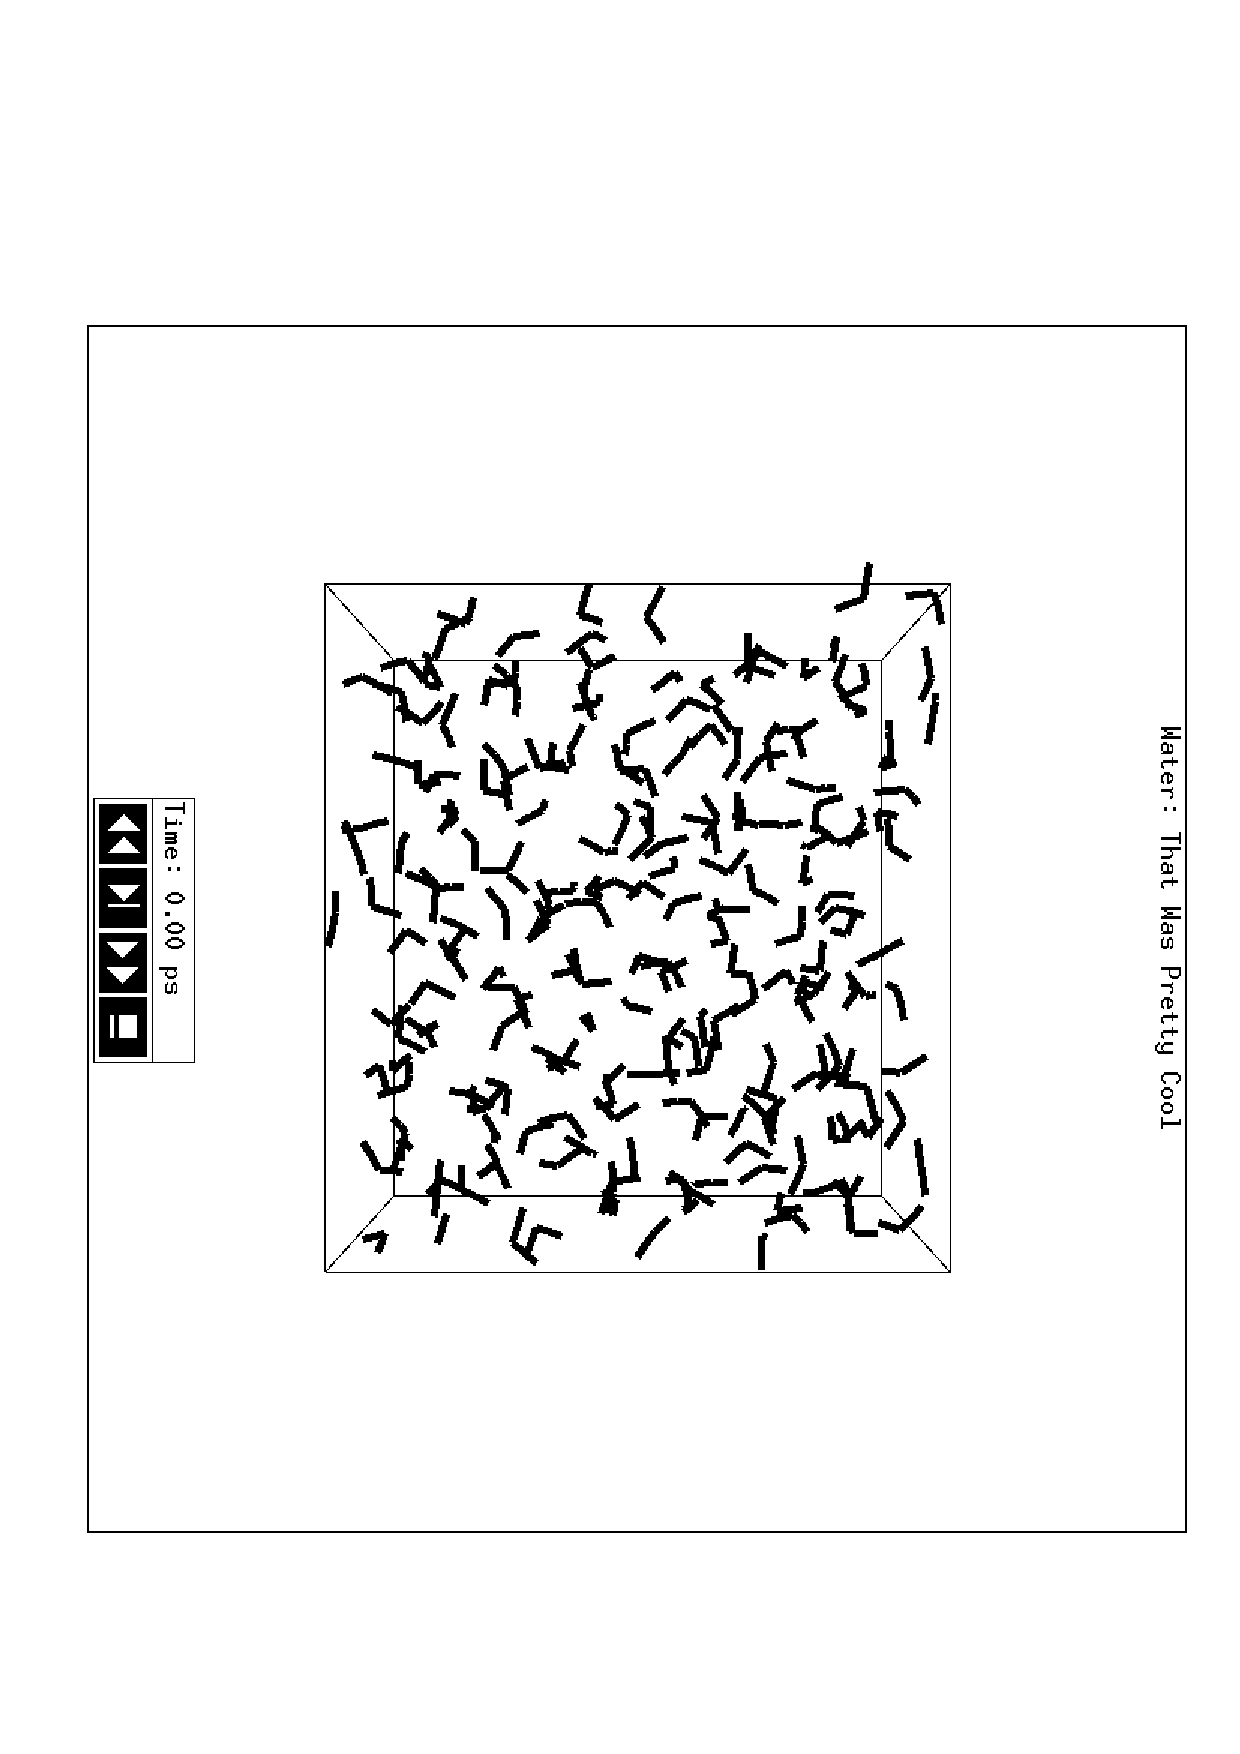
\includegraphics[width=8cm,angle=90]{plots/ngmxdump}}}
\caption{The window of {\tt ngmx} showing a box of water.}
\label{fig:ngmxdump}
\end{figure}

Before analyzing your trajectory it is often informative to look at
your trajectory first. {\gromacs} comes with a simple trajectory
viewer {\tt \normindex{ngmx}}; the advantage with this one is that it does not
require OpenGL, which usually isn't present on {\eg} supercomputers.
It is also possible to generate a
hard-copy in Encapsulated Postscript format (see
\figref{ngmxdump}). If you want a faster and more fancy viewer
 there are several programs
that can read the {\gromacs} trajectory formats -- have a look at our
homepage ({\wwwpage}) for updated links. 

%%%%%%%%%%%%%%%%%%%%%%%%%%%%%%%%%%%%%%% General properties

\section{General properties}
\label{sec:genprop}
{\tt g_energy, g_traj}\\
To analyze some or all {\em energies} and other properties, such as
{\em total pressure}, {\em pressure tensor}, {\em density}, {\em
box-volume} and {\em box-sizes}, use the program {\tt \normindex{g_energy}}.  A
choice can be made from a list a set of energies, like potential,
kinetic or total energy, or individual contributions, like
Lennard-Jones or dihedral energies.

The {\em center-of-mass velocity}, defined as
\beq
{\bf v}_{com} = {1 \over M} \sum_{i=1}^N m_i {\bf v}_i
\eeq
with $M = \sum_{i=1}^N m_i$ the total mass of the system, can be
monitored in time by the program {\tt \normindex{g_traj} -com -ov}. It is however
recommended to remove the center-of-mass velocity every step (see
\chref{algorithms})!

%%%%%%%%%%%%%%%%%%%%%%%%%%%%%%%%%%%%%%% Radial distribution functions 

\section{Radial distribution functions}
\label{sec:rdf}
{\tt g_rdf}\\
The {\em radial distribution function} (RDF) or pair correlation
function $g_{AB}(r)$ between particles of type $A$ and $B$ is defined
in the following way:
\newcommand{\dfrac}[2]{\displaystyle \frac{#1}{#2}}
\beq
\begin{array}{rcl}
g_{AB}(r)&=&    \dfrac{\langle \rho_B(r) \rangle}{\langle\rho_B\rangle_{local}}         \\
         &=&    \dfrac{1}{\langle\rho_B\rangle_{local}}\dfrac{1}{N_A}
                \sum_{i \in A}^{N_A} \sum_{j \in B}^{N_B} 
                \dfrac{\delta( r_{ij} - r )}{4 \pi r^2}         \\
\end{array}
\eeq
with $\langle\rho_B(r)\rangle$ the particle density of type $B$ at a distance $r$
around particles $A$, and $\langle\rho_B\rangle_{local}$ the particle density of
type $B$ averaged over all spheres around particles $A$ with radius
$r_{max}$ (see \figref{rdfex}C).

\begin{figure}
\centerline{
{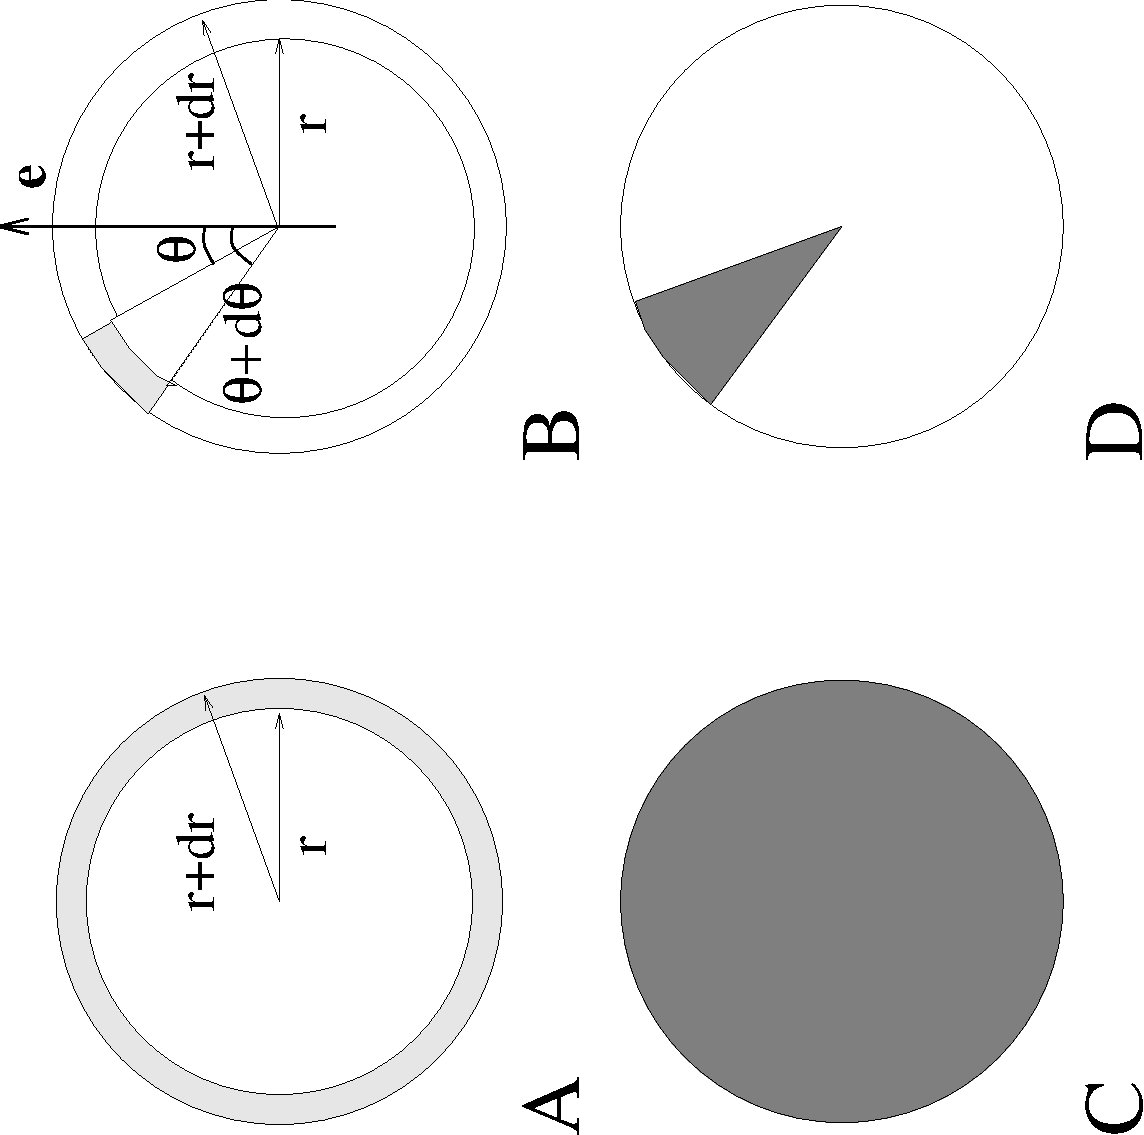
\includegraphics[width=7cm,angle=270]{plots/rdf}}}
\caption[Definition of slices in {\tt g_rdf}.]{Definition of slices
in {\tt g_rdf}: A. $g_{AB}(r)$. B. $g_{AB}(r,\theta)$. The slices are
colored gray. C. Normalization $\langle\rho_B\rangle_{local}$. D. Normalization
$\langle\rho_B\rangle_{local,\:\theta }$. Normalization volumes are colored gray.}
\label{fig:rdfex}
\end{figure}

Usually the value of $r_{max}$ is half of the box length.  The
averaging is also performed in time.  In practice the analysis program
{\tt \normindex{g_rdf}} divides the system into spherical slices (from $r$ to
$r+dr$, see \figref{rdfex}A) and makes a histogram in stead of
the $\delta$-function. An example of the RDF of oxygen-oxygen in
SPC water~\cite{Berendsen81} is given in \figref{rdf}.

\begin{figure}
\centerline{
{\includegraphics[width=8cm]{plots/rdfO-O}}}
\caption{$g_{OO}(r)$ for Oxygen-Oxygen of SPC-water.}
\label{fig:rdf}
\end{figure}

With {\tt g_rdf} it is also possible to calculate an angle dependent rdf 
$g_{AB}(r,\theta)$, where the angle $\theta$ is defined with respect to a 
certain laboratory axis ${\bf e}$, see \figref{rdfex}B.
\bea 
g_{AB}(r,\theta) &=& {1 \over \langle\rho_B\rangle_{local,\:\theta }} {1 \over N_A} \sum_{i \in A}^{N_A} \sum_{j \in B}^{N_B} {\delta( r_{ij} - r ) \delta(\theta_{ij} -\theta) \over 2 \pi r^2 sin(\theta)}\\
cos(\theta_{ij}) &=& {{\bf r}_{ij} \cdot {\bf e} \over \|r_{ij}\| \;\| e\| }
\eea
This $g_{AB}(r,\theta)$ is useful for analyzing anisotropic systems. 
{\bf Note} that in this case the normalization $\langle\rho_B\rangle_{local,\:\theta}$ is 
the average density in all angle slices from $\theta$ to $\theta + d\theta$ 
up to $r_{max}$, so angle dependent, see \figref{rdfex}D.

%%%%%%%%%%%%%%%%%%%%%%%%%%%%%%%%%%%%%%% Correlation functions 
%\ifthenelse{\equal{\gmxlite}{1}}{}{

\section{Correlation functions}
\label{sec:corr}

\subsection{Theory of correlation functions}
The theory of correlation functions is well established~\cite{Allen87}.
We describe here the implementation of the various 
\normindex{correlation} function flavors in the {\gromacs} code.
The definition of the \swapindex{autocorrelation}{function} (ACF)
$C_f(t)$ for a property $f(t)$ is:
\beq
C_f(t)  ~=~     \left\langle f(\xi) f(\xi+t)\right\rangle_{\xi}
\label{eqn:corr}
\eeq
where the notation on the right hand side indicates averaging over $\xi$, {\ie} over
time origins.
It is also possible to compute cross-correlation function from two properties
$f(t)$ and $g(t)$:
\beq
C_{fg}(t) ~=~   \left\langle f(\xi) g(\xi+t)\right\rangle_{\xi}
\eeq
however, in {\gromacs} there is no standard mechanism to do this
({\bf note:} you can use the {\tt \normindex{xmgr}} program to compute cross correlations).
The integral of the correlation function over time is the 
correlation time $\tau_f$:
\beq
\tau_f  ~=~     \int_0^{\infty} C_f(t) {\rm d} t
\label{eqn:corrtime}
\eeq

In practice, correlation functions are calculated based on data points with
discrete time intervals {$\Delta$t}, so that the ACF from an MD simulation is:
\beq
C_f(j\Delta t)  ~=~     \frac{1}{N-j}\sum_{i=0}^{N-1-j} f(i\Delta t) f((i+j)\Delta t)
\label{eqn:corrmd}
\eeq
where $N$ is the number of available time frames for the calculation.
The resulting ACF is
obviously only available at time points with the same interval {$\Delta$t}.
Since, for many applications, it is necessary to know the short time behavior
of the ACF ({\eg} the first 10 ps) this often means that we have to save the
data with intervals much shorter than the time scale of interest.
Another implication of \eqnref{corrmd} is that in principle we can not compute
all points of the ACF with the same accuracy, since we have $N-1$ data points
for $C_f(\Delta t)$ but only 1 for $C_f((N-1)\Delta t)$. However, if we decide to
compute only an ACF of length $M\Delta t$, where $M \leq N/2$ we can compute 
all points with the same statistical accuracy:
\beq
C_f(j\Delta t)  ~=~ \frac{1}{M}\sum_{i=0}^{N-1-M} f(i\Delta t)f((i+j)\Delta t)
\eeq
Here of course $j < M$.
$M$ is sometimes referred to as the \normindex{time lag} of the correlation function. 
When we decide to do this, we intentionally do not use all the available points
for very short time intervals ($j << M$), but it makes it easier to interpret
the results.
Another aspect that may not be neglected when computing
ACFs from simulation is that usually the time origins $\xi$ (\eqnref{corr})
are not statistically independent, which may introduce a bias in the results.
This can be tested using a block-averaging procedure, where only time origins
with a spacing at least the length of the time lag are included, {\eg} using 
$k$ time origins with spacing of $M\Delta t$ (where $kM \leq N$):
\beq
C_f(j\Delta t)  ~=~ \frac{1}{k}\sum_{i=0}^{k-1} f(iM\Delta t)f((iM+j)\Delta t)
\eeq
However, one
needs very long simulations to get good accuracy this way, because there are 
many fewer points that contribute to the ACF.

\subsection{Using FFT for computation of the ACF}
The computational cost for calculating an ACF according to \eqnref{corrmd}
is proportional to $N^2$, which is considerable. However, this can be improved
by using fast Fourier transforms to do the convolution~\cite{Allen87}.

\subsection{Special forms of the ACF}
There are some important varieties on the ACF, {\eg} the ACF of a vector \ve{p}:
\beq
C_{\ve{p}}(t) ~=~       \int_0^{\infty} P_n(\cos\angle\left(\ve{p}(\xi),\ve{p}(\xi+t)\right) {\rm d} \xi
\label{eqn:corrleg}
\eeq
where $P_n(x)$ is the $n^{th}$ order Legendre polynomial
\footnote{$P_0(x) = 1$, $P_1(x) = x$, $P_2(x) = (3x^2-1)/2$}.
Such correlation times 
can actually be obtained experimentally using {\eg} NMR or other relaxation 
experiments. {\gromacs} can compute correlations using 
the 1$^{st}$ and 2$^{nd}$ order Legendre polynomial (\eqnref{corrleg}).
This can also be used for rotational autocorrelation ({\tt \normindex{g_rotacf}}) 
and dipole autocorrelation ({\tt \normindex{g_dipoles}}).

In order to study torsion angle dynamics, we define a dihedral 
autocorrelation function as~\cite{Spoel97a}:
\beq
C(t)    ~=~     \left\langle \cos(\theta(\tau)-\theta(\tau+t))\right\rangle_{\tau}
\label{eqn:coenk}
\eeq
{\bf Note} that this is not a  product of two functions 
as is generally used for correlation
functions, but it may be rewritten as the sum of two products:
\beq
C(t)    ~=~     \left\langle\cos(\theta(\tau))\cos(\theta(\tau+t))\,+\,\sin(\theta(\tau))\sin(\theta(\tau+t))\right\rangle_{\tau}
\label{eqn:cot}
\eeq

\subsection{Some Applications}
The program {\tt \normindex{g_velacc}} calculates the {\em velocity autocorrelation 
function}.
\beq
C_{\ve{v}} (\tau) ~=~ \langle {\ve{v}}_i(\tau) \cdot {\ve{v}}_i(0) \rangle_{i \in A}
\eeq
The self diffusion coefficient can be calculated using the Green-Kubo 
relation~\cite{Allen87}:
\beq
D_A ~=~ {1\over 3} \int_0^{\infty} \langle {\bf v}_i(t) \cdot {\bf v}_i(0) \rangle_{i \in A} \; dt
\eeq
which is just the integral of the velocity autocorrelation function.
There is a widely-held belief that the velocity ACF converges faster than the mean
square displacement (\secref{msd}), which can also be used for the computation of 
diffusion constants. However, Allen \& Tildesley~\cite{Allen87} 
warn us that the long-time 
contribution to the velocity ACF can not be ignored, so care must be taken.

Another important quantity is the dipole correlation time. The {\em dipole 
correlation function} for particles of type $A$ is calculated as follows by 
{\tt \normindex{g_dipoles}}:
\beq
C_{\mu} (\tau) ~=~
\langle {\bf \mu}_i(\tau) \cdot {\bf \mu}_i(0) \rangle_{i \in A}
\eeq
with ${\bf \mu}_i = \sum_{j \in i} {\bf r}_j q_j$. The dipole correlation time 
can be computed using \eqnref{corrtime}.
For some applications see~\cite{Spoel98a}.

The \normindex{viscosity} of a liquid can be related to the correlation 
time of the Pressure tensor $\ve{P}$~\cite{PSmith93c,Balasubramanian96}.
{\tt \normindex{g_energy}} can compute the viscosity,
but this is not very accurate~\cite{Hess2002a}, and 
actually the values do not converge.
%} % Brace matches ifthenelse test for gmxlite

\section{Mean Square Displacement}
\label{sec:msd}
{\tt g_msd}\\
To determine the self \swapindex{diffusion}{coefficient} $D_A$ of
particles of type $A$, one can use the \normindex{Einstein
relation}~\cite{Allen87}:
\beq 
\lim_{t \rightarrow \infty} \langle
\|{\bf r}_i(t) - {\bf r}_i(0)\|^2 \rangle_{i \in A} ~=~ 6 D_A t 
\eeq
This {\em mean square displacement} and $D_A$ are calculated by the
program {\tt \normindex{g_msd}}. Normally an index file containing
atom numbers is used and the MSD is averaged over these atoms.  For
molecules consisting of more than one atom, ${\bf r}_i$ can be taken
as the center of mass positions of the molecules. In that case, you
should use an index file with molecule numbers. The results will be
nearly identical to averaging over atoms, however. The {\tt g_msd}
program can
also be used for calculating diffusion in one or two dimensions. This
is useful for studying lateral diffusion on interfaces.

An example of the mean square displacement of SPC water is given in
\figref{msdwater}.

\begin{figure}
\centerline{
{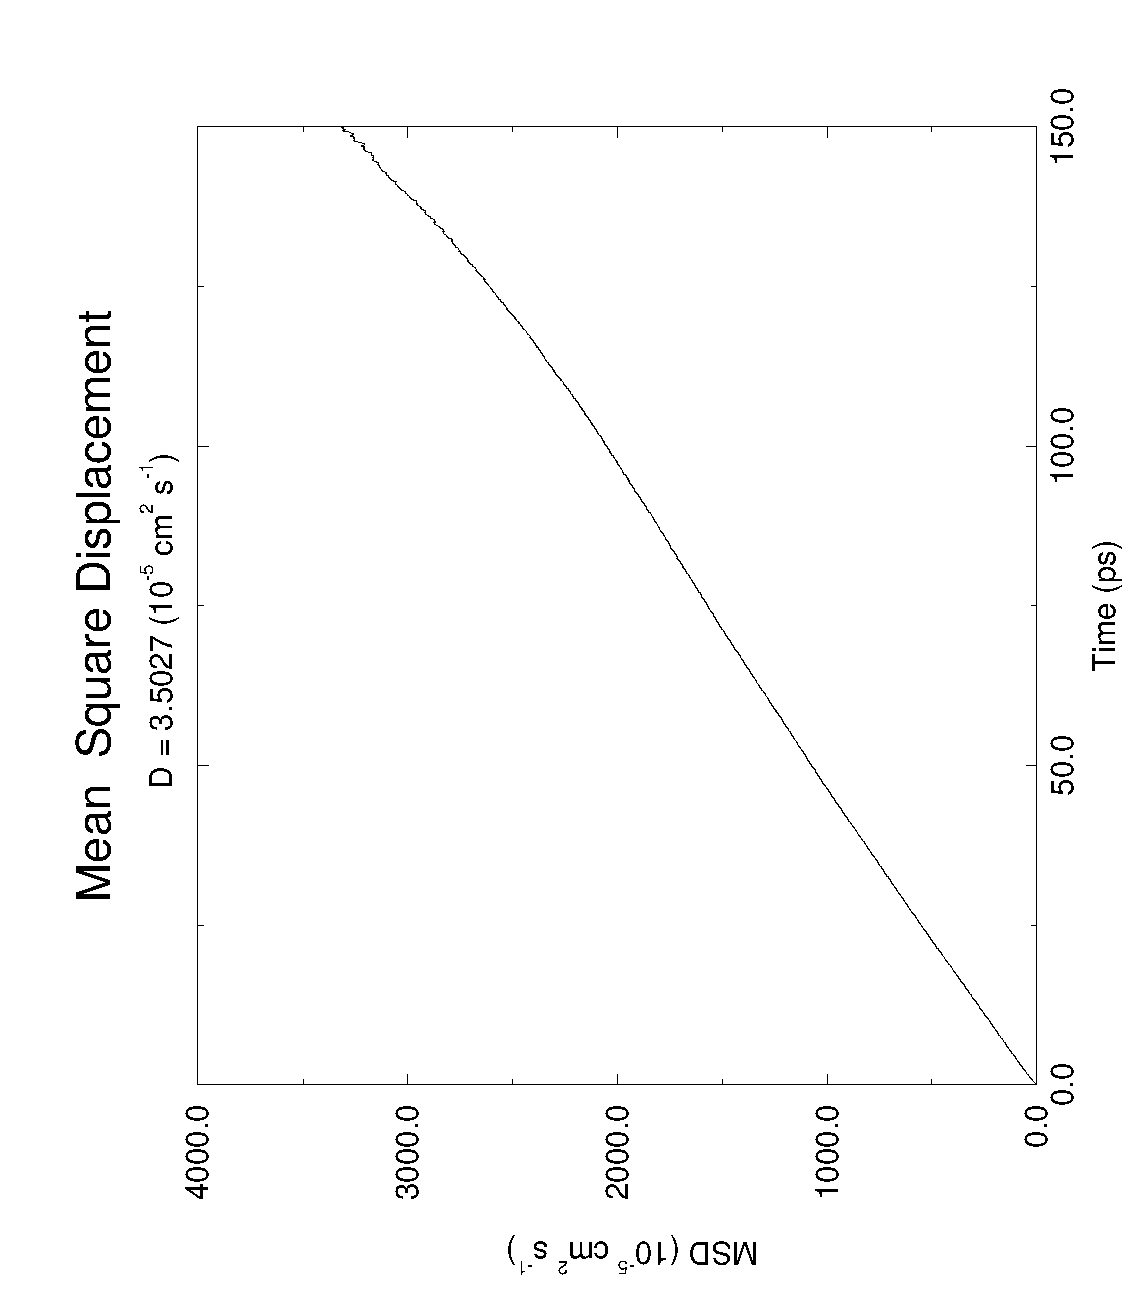
\includegraphics[width=8cm]{plots/msdwater}}}
\caption{Mean Square Displacement of SPC-water.}
\label{fig:msdwater}
\end{figure}

%\ifthenelse{\equal{\gmxlite}{1}}{}{
% 
%%%%%%%%%%%%%%%%%%%%% Bonds, angles and dihedral %%%%%%%%%%%%%%%%%%%
% 
\section{Bonds, angles and dihedrals}
\label{sec:bad}
{\tt g_bond, g_angle, g_sgangle}\\
To monitor specific {\em bonds} in your molecules during time, the program 
{\tt \normindex{g_bond}} calculates the distribution of the bond length in time. 
The index file consists of pairs of atom numbers, for example\\

\begin{verbatim}
[ bonds_1 ]
 1     2
 3     4
 9    10

[ bonds_2 ]
12    13
\end{verbatim}

The program {\tt \normindex{g_angle}} calculates the distribution of {\em angles} and 
{\em dihedrals} in time. It also gives the average angle or dihedral. 
The index file consists of triplets or quadruples of atom numbers:

\begin{verbatim}
[ angles ]
 1     2     3
 2     3     4
 3     4     5

[ dihedrals ]
 1     2     3     4
 2     3     5     5
\end{verbatim}

For the dihedral angles you can use either the ``biochemical convention'' 
($\phi = 0 \equiv cis$) or ``polymer convention'' ($\phi = 0 \equiv trans$), 
see \figref{dih_def}.

\begin{figure}
\centerline{
{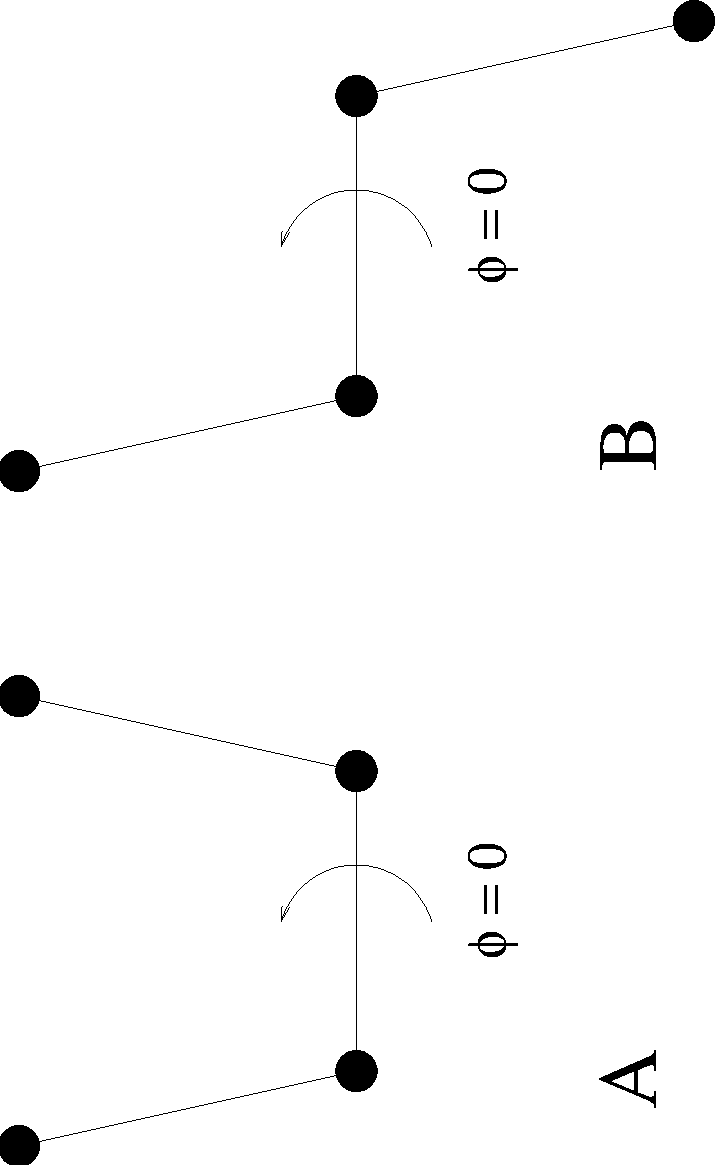
\includegraphics[width=3.5cm,angle=270]{plots/dih-def}}}
\caption[Dihedral conventions.]{Dihedral conventions: A. ``Biochemical
convention''. B. ``Polymer convention''.}
\label{fig:dih_def}
\end{figure}

To follow specific {\em angles} in time between two vectors, a vector
and a plane or two planes (defined by 2 or 3 atoms, respectively, inside your
molecule, see \figref{sgangle}A, B, C), use the program {\tt \normindex{g_sgangle}}.

\begin{figure}
\centerline{
{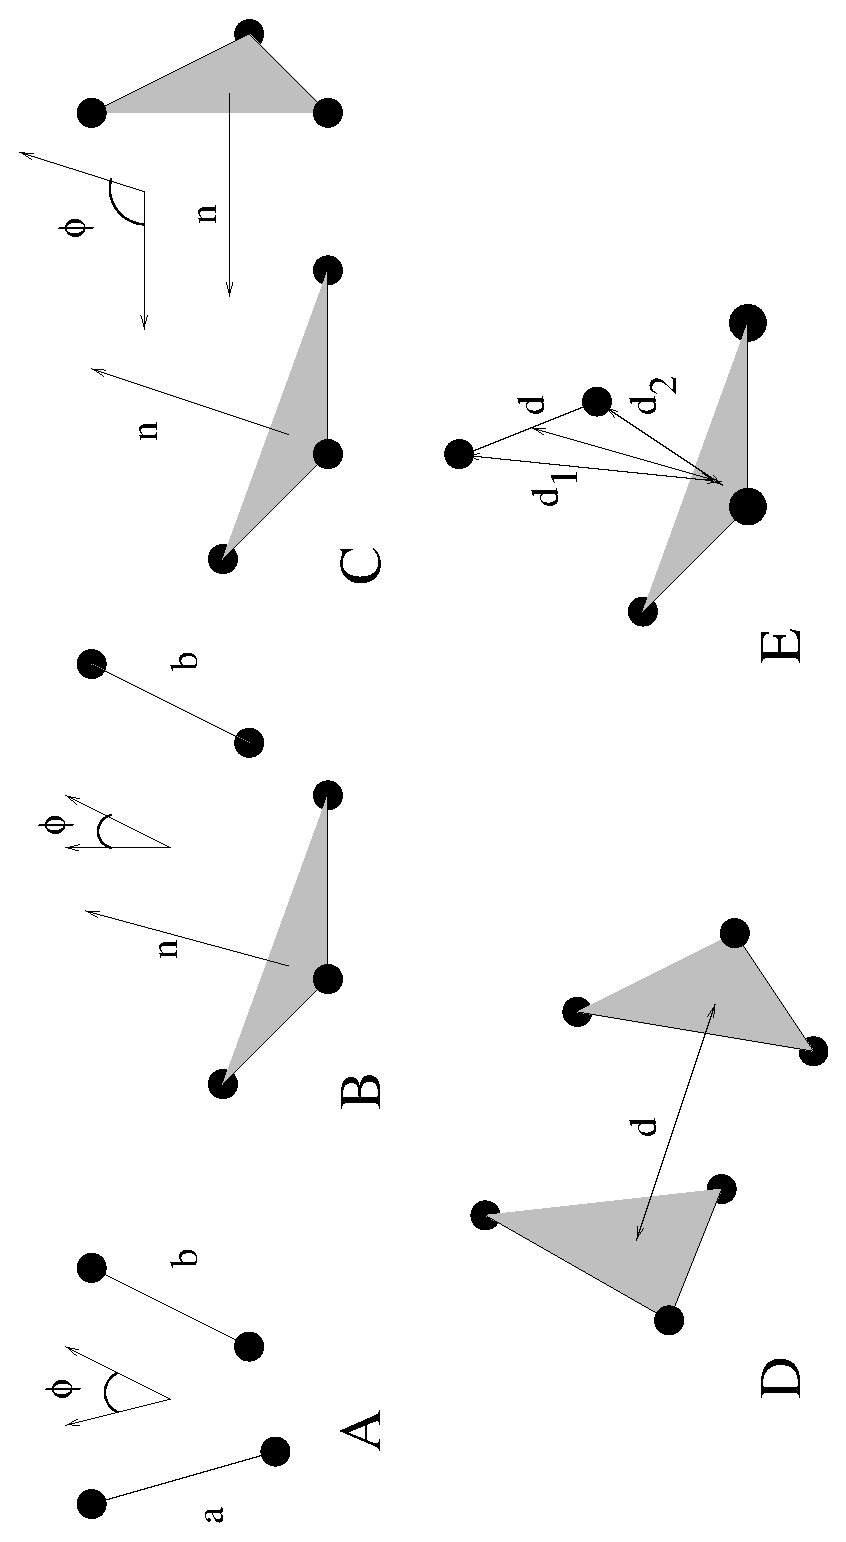
\includegraphics[width=6.5cm,angle=270]{plots/sgangle}}}
\caption[Options of {\tt g_sgangle}.]{Options of {\tt g_sgangle}: A. Angle between 2 vectors. B. Angle between a vector and the normal of a plane. C. Angle between two planes. D. Distance between the geometrical centers of 2 planes. E. Distances between a vector and the center of a plane.}
\label{fig:sgangle}
\end{figure}

For planes, {\tt \normindex{g_sgangle}} uses the normal vector perpendicular to the plane.  It
can also calculate the {\em distance} $d$ between the geometrical
center of two planes (see \figref{sgangle}D), and the distances
$d_1$ and $d_2$ between 2 atoms (of a vector) and the center of a
plane defined by 3 atoms (see \figref{sgangle}D). It further
calculates the distance $d$ between the center of the plane and the
middle of this vector.  Depending on the input groups ({\ie} groups of
2 or 3 atom numbers), the program decides what angles and distances to
calculate. For example, the index-file could look like this:

\begin{verbatim}
[ a_plane ]
 1     2     3

[ a_vector ]
 4     5
\end{verbatim}
%} % Brace matches ifthenelse test for gmxlite

%%%%%%%%%%%%%%%%%%%%%%%%%%%%%%%%%%%%%%% Radius of gyration and distances

\section{Radius of gyration and distances}
\label{sec:rg}
{\tt g_gyrate, g_sgangle, g_mindist, g_mdmat, xpm2ps}\\
To have a rough measure for the compactness of a structure, you can calculate 
the {\em radius of gyration} with the program {\tt \normindex{g_gyrate}} as follows:
\beq
R_g ~=~ \left({\frac{\sum_i \|{\bf r}_i\|^2 m_i}{\sum_i m_i}}\right)^{\half}
\label{eqn:rg}
\eeq
where $m_i$ is the mass of atom $i$ and ${\bf r}_i$ the position of 
atom $i$ with respect to the center of mass of the molecule. It is especially 
useful to characterize polymer solutions and proteins.

Sometimes it is interesting to plot the {\em distance} between two atoms,
or the {\em minimum} distance between two groups of atoms
({\eg}: protein side-chains in a salt bridge). 
To calculate these distances between certain groups there are several 
possibilities:
\begin{description}
\item[$\bullet$] 
The {\em distance between the geometrical centers} of two groups can be 
calculated with the program
%\ifthenelse{\equal{\gmxlite}{1}}{
%{\tt \normindex{g_sgangle}}.}
{{\tt \normindex{g_sgangle}}, as explained in \secref{bad}.}
\item[$\bullet$] 
The {\em minimum distance} between two groups of atoms during time 
can be calculated with the program {\tt \normindex{g_mindist}}. It also calculates the 
{\em number of contacts} between these groups 
within a certain radius $r_{max}$.
\item[$\bullet$] 
To monitor the {\em minimum distances between amino acid residues} 
within a (protein) molecule, you can use 
the program {\tt \normindex{g_mdmat}}. This minimum distance between two residues
A$_i$ and A$_j$ is defined as the smallest distance between any pair of 
atoms (i $\in$ A$_i$, j $\in$ A$_j$).
The output is a symmetrical matrix of smallest distances 
between all residues.
To visualize this matrix, you can use a program such as {\tt xv}.
If you want to view the axes and legend or if you want to print
the matrix, you can convert it with 
{\tt xpm2ps} into a Postscript picture, see \figref{mdmat}.
\begin{figure}
\centerline{
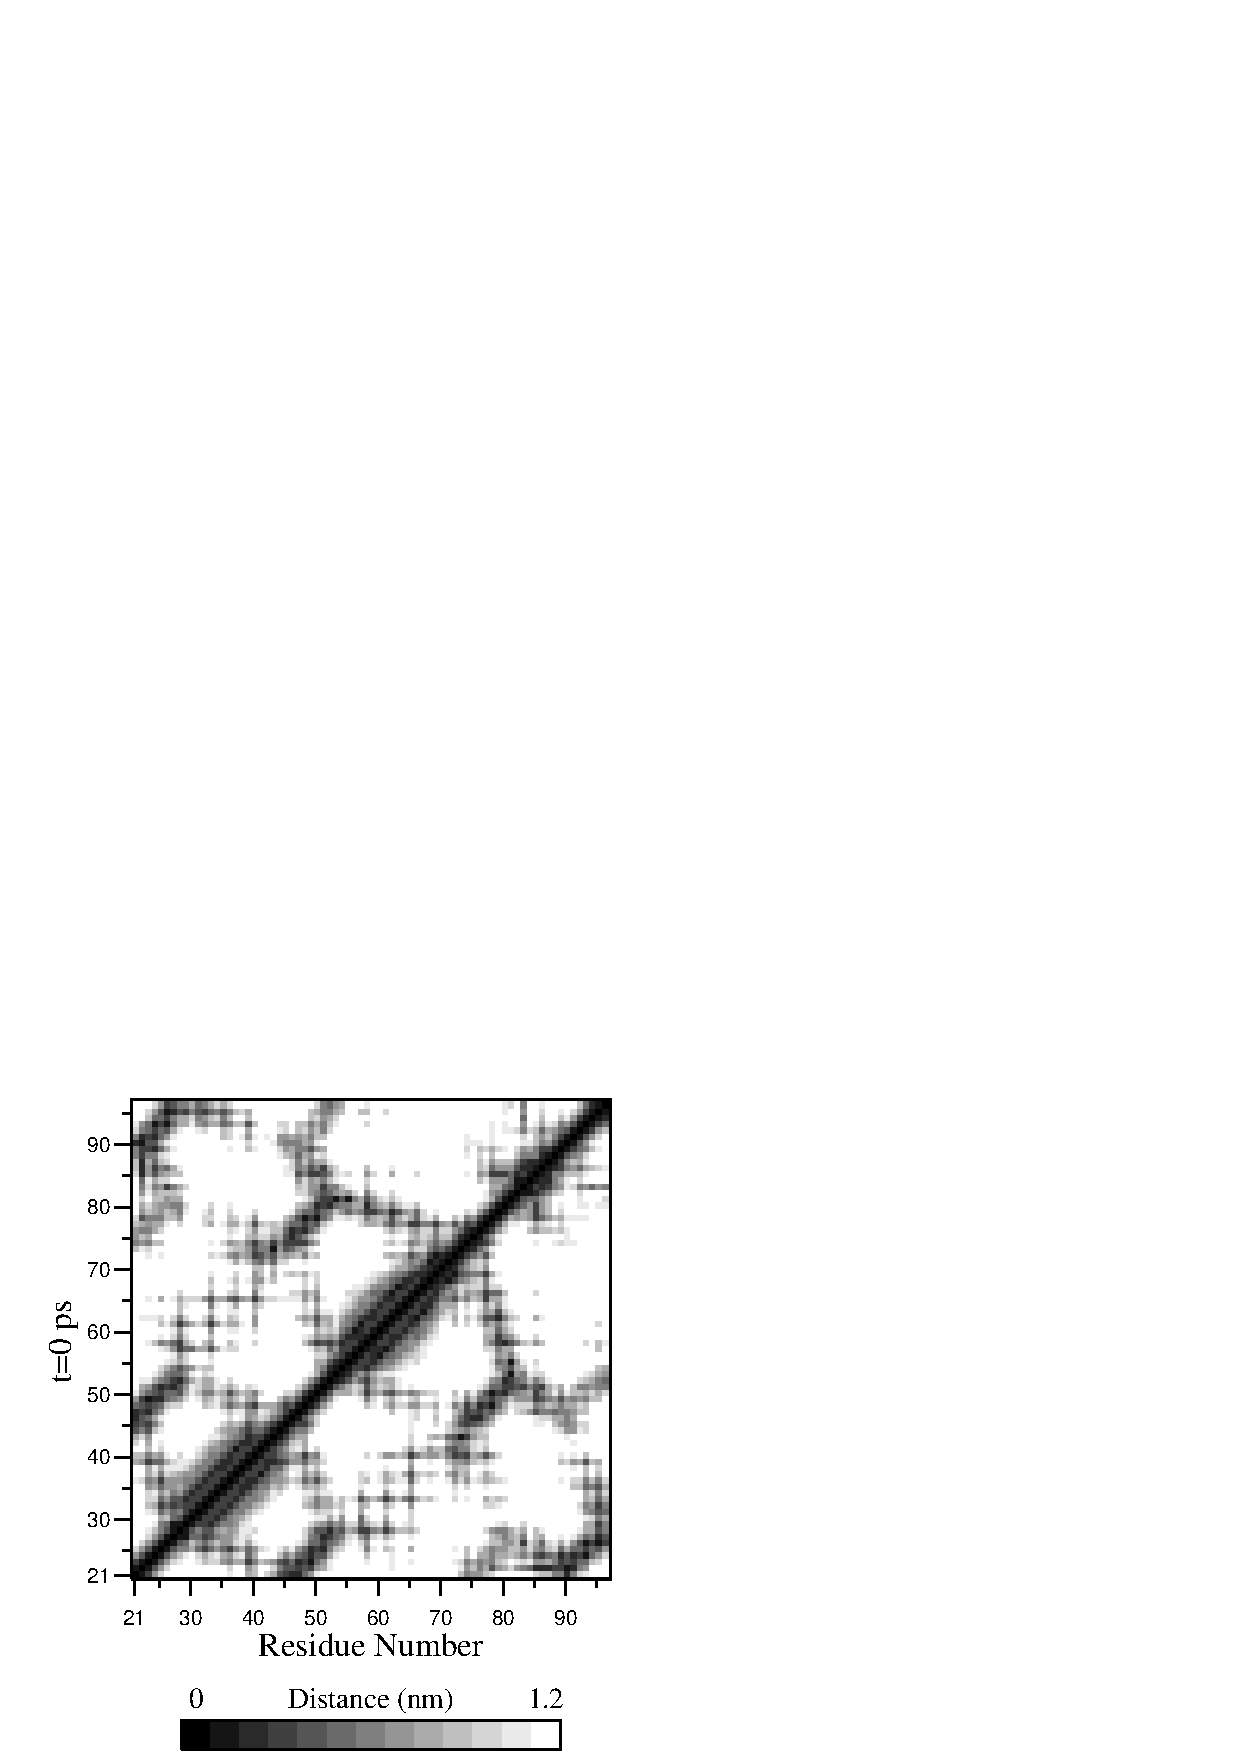
\includegraphics[width=6.5cm]{plots/distm}}
\caption{A minimum distance matrix for a peptide~\protect\cite{Spoel96b}.}
\label{fig:mdmat}
\end{figure}

Plotting these matrices for different time-frames, one can analyze changes 
in the structure, and {\eg} forming of salt bridges.
\end{description}

%%%%%%%%%%%%%%%%%%%%%%%%%%%%%%%%%%%%%%% Root mean square deviations 

\section{Root mean square deviations in structure}
\label{sec:rmsd}
{\tt g_rms, g_rmsdist}\\
The {\em root mean square deviation} ($RMSD$) of certain atoms in a molecule
with respect to a reference structure can be calculated with the program 
{\tt \normindex{g_rms}} by least-square fitting the structure to the reference structure
($t_2 = 0$) and subsequently calculating the $RMSD$ (\eqnref{rmsd}).
\beq
RMSD(t_1,t_2) ~=~ \left[\frac{1}{M} \sum_{i=1}^N m_i \|{\bf r}_i(t_1)-{\bf r}_i(t_2)\|^2 \right]^{\frac{1}{2}}
\label{eqn:rmsd}
\eeq
where $M = \sum_{i=1}^N m_i$ and ${\bf r}_i(t)$ is the position of atom $i$ at time $t$.
{\bf Note} that fitting does not have to use the same atoms as the calculation
of the $RMSD$; {\eg} a protein is usually fitted on the backbone atoms
(N,C$_{\alpha}$,C), but the $RMSD$ can be computed of the backbone
or of the whole protein.

Instead of comparing the structures to the initial structure at time $t=0$ 
(so for example a crystal structure), one can also calculate \eqnref{rmsd} 
with a structure at time $t_2=t_1-\tau$.
This gives some insight in the mobility as a function of $\tau$.
A matrix can also be made with the $RMSD$ as a function of $t_1$ and $t_2$,
which gives a nice graphical interpretation of a trajectory.
If there are transitions in a trajectory, they will clearly show up in
such a matrix.

Alternatively the $RMSD$ can be computed using a fit-free method with the 
program {\tt \normindex{g_rmsdist}}:
\beq
RMSD(t) ~=~     \left[\frac{1}{N^2}\sum_{i=1}^N \sum_{j=1}^N    \|{\bf r}_{ij}(t)-{\bf r}_{ij}(0)\|^2\right]^{\frac{1}{2}}
\label{eqn:rmsdff}
\eeq
where the {\em distance} {\bf r}$_{ij}$ between atoms at time $t$ 
is compared with the distance between the same atoms at time $0$.

%\ifthenelse{\equal{\gmxlite}{1}}{}{
\section{\normindex{Covariance analysis}}
\label{sec:covanal}
Covariance analysis, also called
\seeindex{principal component analysis}{covariance analysis}
or \seeindex{essential dynamics}{covariance analysis}
\cite{Amadei93}{,} can find correlated motions.
It uses the covariance matrix $C$ of the atomic coordinates:
\beq
C_{ij} = \left \langle 
M_{ii}^{\frac{1}{2}} (x_i - \langle x_i \rangle)
M_{jj}^{\frac{1}{2}}  (x_j - \langle x_j \rangle)
\right \rangle
\eeq
where $M$ is a diagonal matrix containing the masses of the atoms
(mass-weighted analysis) or the unit matrix (non-mass weighted analysis).
$C$ is a symmetric $3N \times 3N$ matrix, which can be diagonalized with
an orthonormal transformation matrix $R$:
\beq
R^T C R = \mbox{diag}(\lambda_1,\lambda_2,\ldots,\lambda_{3N})
~~~~\mbox{where}~~\lambda_1 \geq \lambda_2 \geq \ldots \geq \lambda_{3N}
\eeq
The columns of $R$ are the eigenvectors, also called principal or
essential modes.
$R$ defines a transformation to a new coordinate system. The trajectory
can be projected on the principal modes to give the principal components
$p_i(t)$:
\beq
{\bf p}(t) = R^T M^{\frac{1}{2}} ({\bf x}(t) - \langle {\bf x} \rangle)
\eeq
The eigenvalue $\lambda_i$ is the mean square fluctuation of principal
component $i$. The first few principal modes often describe 
collective, global motions in the system.
The trajectory can be filtered along one (or more) principal modes.
For one principal mode $i$ this goes as follows:
\beq
{\bf x}^f(t) =
\langle {\bf x} \rangle + M^{-\frac{1}{2}} R_{*i} \, p_i(t)
\eeq

When the analysis is performed on a macromolecule, one often wants to
remove the overall rotation and translation to look at the internal motion
only. This can be achieved by least square fitting to a reference structure.
Care has to be taken that the reference structure is representative for the
ensemble, since the choice of reference structure influences the covariance
matrix.

One should always check if the principal modes are well defined.
If the first principal component resembles a half cosine and
the second resembles a full cosine, you might be filtering noise (see below).
A good way to check the relevance of the first few principal
modes is to calculate the overlap of the sampling between
the first and second half of the simulation.
{\bf Note} that this can only be done when the same reference structure is
used for the two halves.

A good measure for the overlap has been defined in~\cite{Hess2002b}.
The elements of the covariance matrix are proportional to the square
of the displacement, so we need to take the square root of the matrix
to examine the extent of sampling. The square root can be
calculated from the eigenvalues $\lambda_i$ and the eigenvectors,
which are the columns of the rotation matrix $R$.
For a symmetric and diagonally-dominant matrix $A$ of size $3N \times 3N$
the square root can be calculated as:
\beq
A^\frac{1}{2} = 
R \, \mbox{diag}(\lambda_1^\frac{1}{2},\lambda_2^\frac{1}{2},\ldots,\lambda_{3N}^\frac{1}{2}) \, R^T
\eeq
It can be verified easily that the product of this matrix with itself gives
$A$.
Now we can define a difference $d$ between covariance matrices $A$ and $B$
as follows:
\begin{eqnarray}
d(A,B) & = & \sqrt{\mbox{tr}\left(\left(A^\frac{1}{2} - B^\frac{1}{2}\right)^2\right)
}
\\ & = &
\sqrt{\mbox{tr}\left(A + B - 2 A^\frac{1}{2} B^\frac{1}{2}\right)}
\\ & = &
\left( \sum_{i=1}^N \left( \lambda_i^A + \lambda_i^B \right)
- 2 \sum_{i=1}^N \sum_{j=1}^N \sqrt{\lambda_i^A \lambda_j^B}
\left(R_i^A \cdot R_j^B\right)^2 \right)^\frac{1}{2}
\end{eqnarray}
where tr is the trace of a matrix.
We can now define the overlap $s$ as:
\beq
s(A,B) = 1 - \frac{d(A,B)}{\sqrt{\mbox{tr}A + \mbox{tr} B}}
\eeq
The overlap is 1 if and only if matrices $A$ and $B$ are identical.
It is 0 when the sampled subspaces are completely orthogonal.

A commonly-used measure is the subspace overlap of the first few
eigenvectors of covariance matrices.
The overlap of the subspace spanned by $m$ orthonormal vectors 
${\bf w}_1,\ldots,{\bf w}_m$ with a reference subspace spanned by 
$n$ orthonormal vectors ${\bf v}_1,\ldots,{\bf v}_n$
can be quantified as follows:
\beq
\mbox{overlap}({\bf v},{\bf w}) =
\frac{1}{n} \sum_{i=1}^n \sum_{j=1}^m ({\bf v}_i \cdot {\bf w}_j)^2
\eeq
The overlap will increase with increasing $m$ and will be 1 when
set ${\bf v}$ is a subspace of set ${\bf w}$.
The disadvantage of this method is that it does not take the eigenvalues
into account. All eigenvectors are weighted equally, and when
degenerate subspaces are present (equal eigenvalues), the calculated overlap
will be too low.

Another useful check is the cosine content. It has been proven that the
the principal components of random diffusion are cosines with the number of
periods equal to half the principal component index~\cite{Hess2000,Hess2002b}.
The eigenvalues are proportional to the index to the power $-2$.
The cosine content is defined as:
\beq
\frac{2}{T}
\left( \int_0^T \cos\left(\frac{i \pi t}{T}\right) \, p_i(t) \mbox{d} t \right)^2
\left( \int_0^T p_i^2(t) \mbox{d} t \right)^{-1}
\eeq
When the cosine content of the first few principal components
is close to 1, the largest fluctuations are not connected with
the potential, but with random diffusion.

The covariance matrix is built and diagonalized by
{\tt \normindex{g_covar}}.
The principal components and overlap (and many more things)
can be plotted and analyzed with {\tt \normindex{g_anaeig}}.
The cosine content can be calculated with {\tt \normindex{g_analyze}}.
%} % Brace matches ifthenelse test for gmxlite

%\ifthenelse{\equal{\gmxlite}{1}}{}{
\section{Dihedral principal component analysis}
{\tt g_angle, g_covar, g_anaeig}\\
Principal component analysis can be performed in dihedral
space~\cite{Mu2005a} using {\gromacs}. You start by defining the
dihedral angles of interest in an index file, either using {\tt
  mk_angndx} or otherwise. Then you use the {\tt g_angle} program
with the {\tt -or} flag to produce a new {\tt .trr} file containing the cosine and
sine of each dihedral angle in two coordinates, respectively. That is,
in the {\tt .trr} file you will have a series of numbers corresponding to:
cos($\phi_1$), sin($\phi_1$), cos($\phi_2$), sin($\phi_2$), ...,
cos($\phi_n$), sin($\phi_n$), and the array is padded with zeros, if
necessary.  Then you can use this {\tt .trr} file as input for the {\tt
  g_covar} program and perform principal component analysis as usual.
For this to work you will need to generate a reference file ({\tt .tpr}, 
{\tt .gro}, {\tt .pdb} etc.) containing the same number of ``atoms'' 
as the new {\tt .trr} file, that is for $n$ dihedrals you need 2$n$/3 atoms 
(rounded up if not an integer number). 
You should use the {\tt -nofit} option for {\tt
  g_covar} since the coordinates in the dummy reference file do not
correspond in any way to the information in the {\tt .trr} file. Analysis of
the results is done using {\tt g_anaeig}.  
%} % Brace matches ifthenelse test for gmxlite
 
%%%%%%%%%%%%%%%%%%%%%%%%%%%%%%%%%%%%%%% Hydrogen bonds

\section{Hydrogen bonds}
{\tt g_hbond}\\
The program {\tt \normindex{g_hbond}} analyses the {\em hydrogen bonds} (H-bonds)
between all possible donors D and acceptors A. To determine if an
H-bond exists, a geometrical criterion is used, see also
\figref{hbond}:
\beq
\begin{array}{rclcl}
r       & \leq  & r_{HB}        & = & 0.35~\mbox{nm}    \\
\alpha  & \leq  & \alpha_{HB}   & = & 30^o              \\
\end{array}
\eeq

\begin{figure}
\centerline{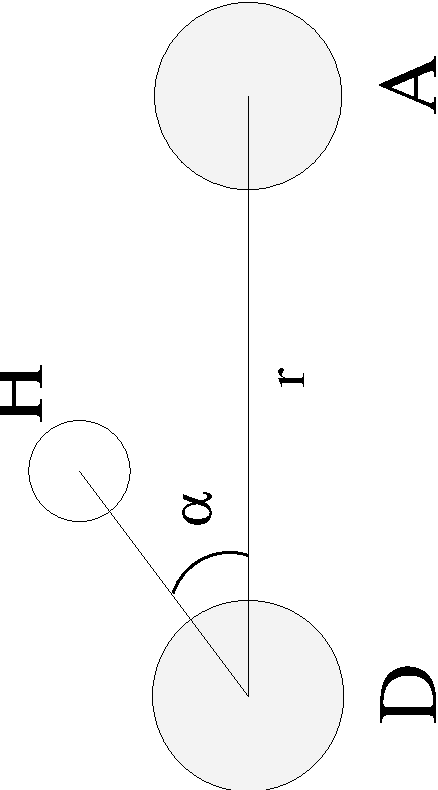
\includegraphics[width=2.5cm,angle=270]{plots/hbond}}
\caption{Geometrical Hydrogen bond criterion.}
\label{fig:hbond}
\end{figure}

The value of $r_{HB} = 0.35$~nm corresponds to the first minimum of the RDF of 
SPC water (see also \figref{rdf}).

The program {\tt g_hbond} analyses all hydrogen bonds existing
between two groups of atoms (which must be either identical or
non-overlapping) or in specified donor-hydrogen-acceptor triplets, in
the following ways:

\begin{figure}
\centerline{
{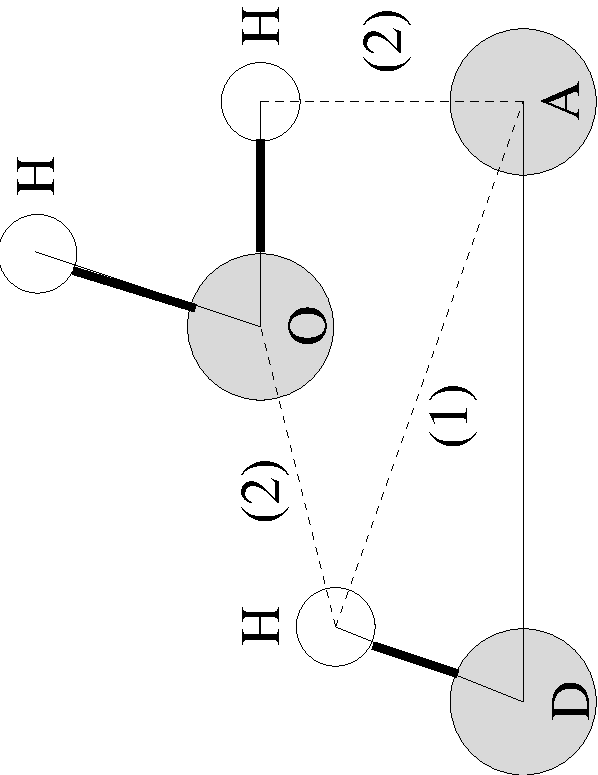
\includegraphics[width=5cm,angle=270]{plots/hbond-insert}}}
\caption[Insertion of water into an H-bond.]{Insertion of water into
an H-bond. (1) Normal H-bond between two residues. (2) H-bonding
bridge via a water molecule.}
\label{fig:insert}
\end{figure}

\begin{itemize}
\item
Donor-Acceptor distance ($r$) distribution of all H-bonds
\item
Hydrogen-Donor-Acceptor angle ($\alpha$) distribution of all H-bonds 
\item
The total number of H-bonds in each time frame
\item
\newcommand{\nn}[1]{$n$-$n$+$#1$}
The number of H-bonds in time between residues, divided into groups
\nn{i} where $n$ and $n$+$i$ stand for residue numbers and $i$ goes
from 0 to 6. The group for $i=6$ also includes all H-bonds for
$i>6$. These groups include the \nn{3}, \nn{4} and \nn{5} H-bonds,
which provide a measure for the formation of $\alpha$-helices or
$\beta$-turns or strands.
\item
The lifetime of the H-bonds is calculated from the average over all
autocorrelation functions of the existence functions (either 0 or 1)
of all H-bonds:
\beq
C(\tau) ~=~ \langle s_i(t)~s_i (t + \tau) \rangle
\label{eqn:hbcorr}
\eeq
with $s_i(t) = \{0,1\}$ for H-bond $i$ at time $t$. The integral of
$C(\tau)$ gives a rough estimate of the average H-bond lifetime
$\tau_{HB}$:
\beq
\tau_{HB} ~=~ \int_{0}^{\infty} C(\tau) d\tau
\label{eqn:hblife}
\eeq
Both the integral and the complete autocorrelation function $C(\tau)$
will be output, so that more sophisticated analysis ({\eg}\@ using
multi-exponential fits) can be used to get better estimates for
$\tau_{HB}$. A more complete analysis is given in ref.~\cite{Spoel2006b};
one of the more fancy option is the Luzar and Chandler analysis
of hydrogen bond kinetics~\cite{Luzar96b,Luzar2000a}. 
\item
An H-bond existence map can be generated of dimensions {\em
\#~H-bonds}$\times${\em \#~frames}. The ordering is identical to the index 
file (see below), but reversed, meaning that the last triplet in the index
file corresponds to the first row of the existence map.
\item
Index groups are output containing the analyzed groups, all
donor-hydrogen atom pairs and acceptor atoms in these groups,
donor-hydrogen-acceptor triplets involved in hydrogen bonds between
the analyzed groups and all solvent atoms involved in insertion.

% The {\tt -ins} option appears to have been removed during the course of version 4.5 development
% \item
% Solvent insertion into H-bonds can be analyzed, see
% \figref{insert}. In this case an additional group identifying
% the solvent must be selected. The occurrence of insertion will be
% indicated in the existence map. {\bf Note} that insertion into and existence
% of a specific H-bond can occur simultaneously and will also be
% indicated as such in the existence map.

\end{itemize}

%\ifthenelse{\equal{\gmxlite}{1}}{}{
%
%%%%%%%%%%%%%%%%%%%%%%%%%%%%%%%%%%%%%%% Protein related items 

\section{Protein-related items}
{\tt do_dssp, g_rama, g_xrama, g_wheel}\\
To analyze structural changes of a protein, you can calculate the radius of 
gyration or the minimum residue distances over time 
(see \secref{rg}), or calculate the RMSD (\secref{rmsd}).

You can also look at the changing of {\em secondary structure elements} 
during your run. For this, you can use the program {\tt \normindex{do_dssp}}, which is 
an interface for the commercial program {\tt DSSP}~\cite{Kabsch83}. For 
further information, see the {\tt DSSP} manual. A typical output plot of 
{\tt do_dssp} is given in \figref{dssp}.

\begin{figure}
\centerline{
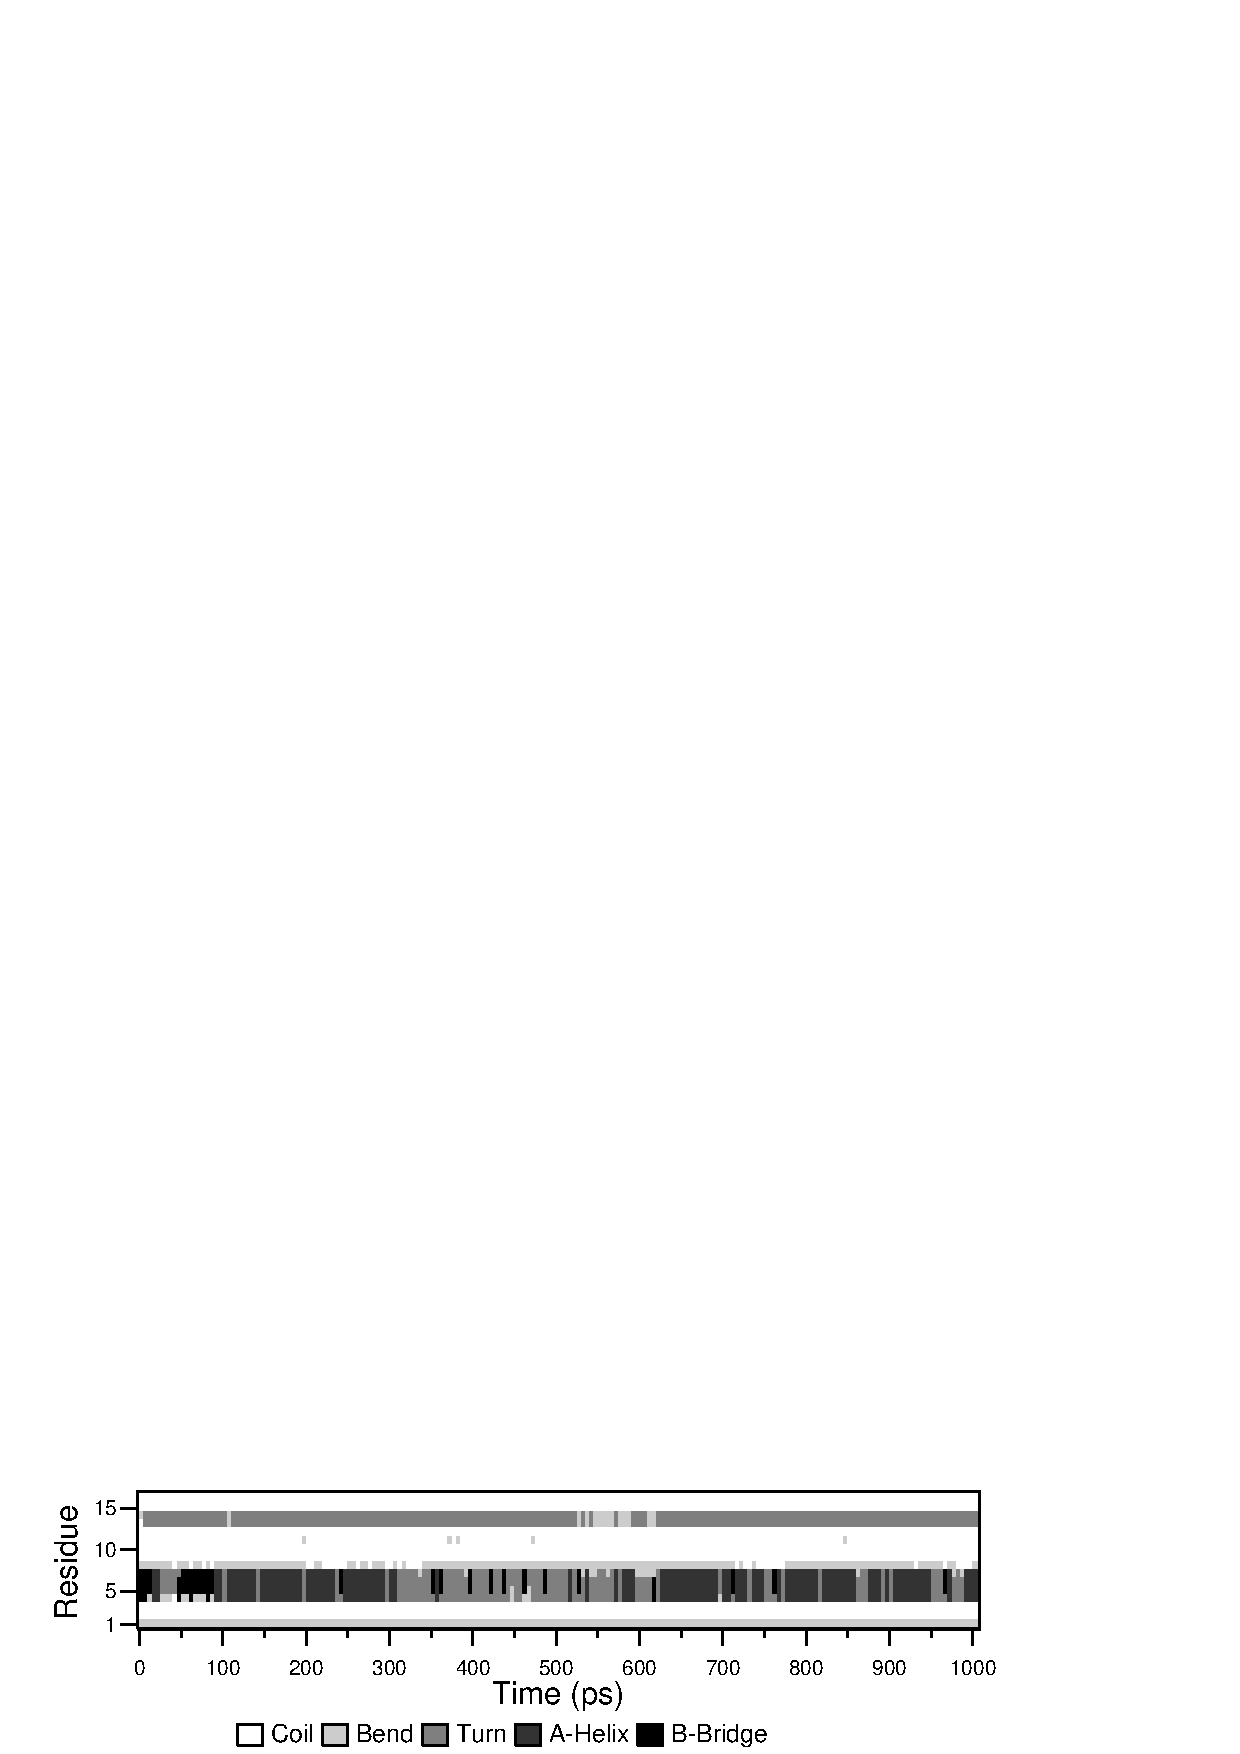
\includegraphics[width=12cm]{plots/dssp}}
\caption{Analysis of the secondary structure elements of a peptide in time.}
\label{fig:dssp}
\end{figure}

One other important analysis of proteins is the so-called 
{\em Ramachandran plot}. 
This is the projection of the structure on the two dihedral angles $\phi$ and 
$\psi$ of the protein backbone, see \figref{phipsi}.

\begin{figure}
\centerline{
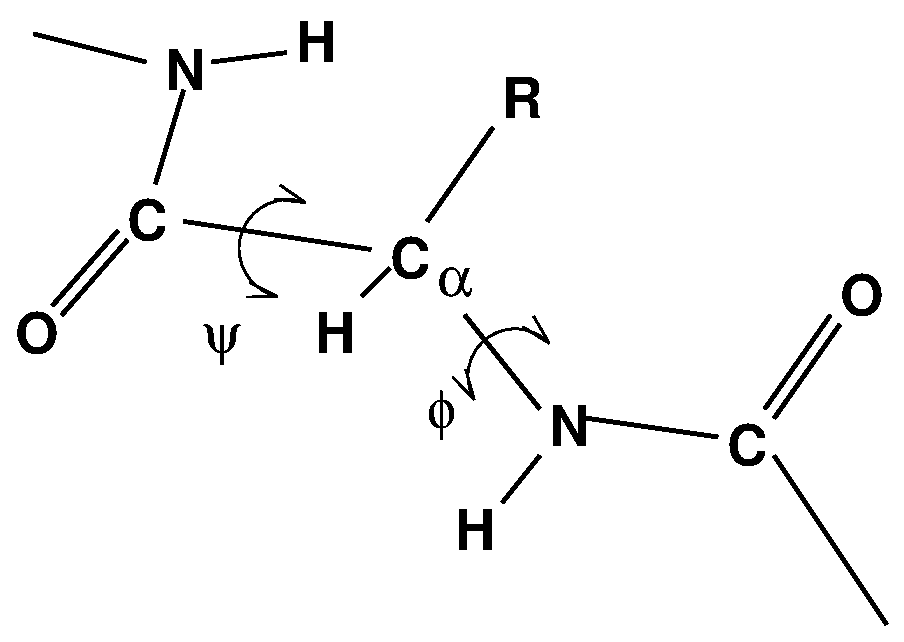
\includegraphics[width=5cm]{plots/phipsi}}
\caption{Definition of the dihedral angles $\phi$ and $\psi$ of the protein backbone.}
\label{fig:phipsi}
\end{figure}

To evaluate this Ramachandran plot you can use the program {\tt \normindex{g_rama}}. 
A typical output is given in \figref{rama}.

\begin{figure}
\centerline{
{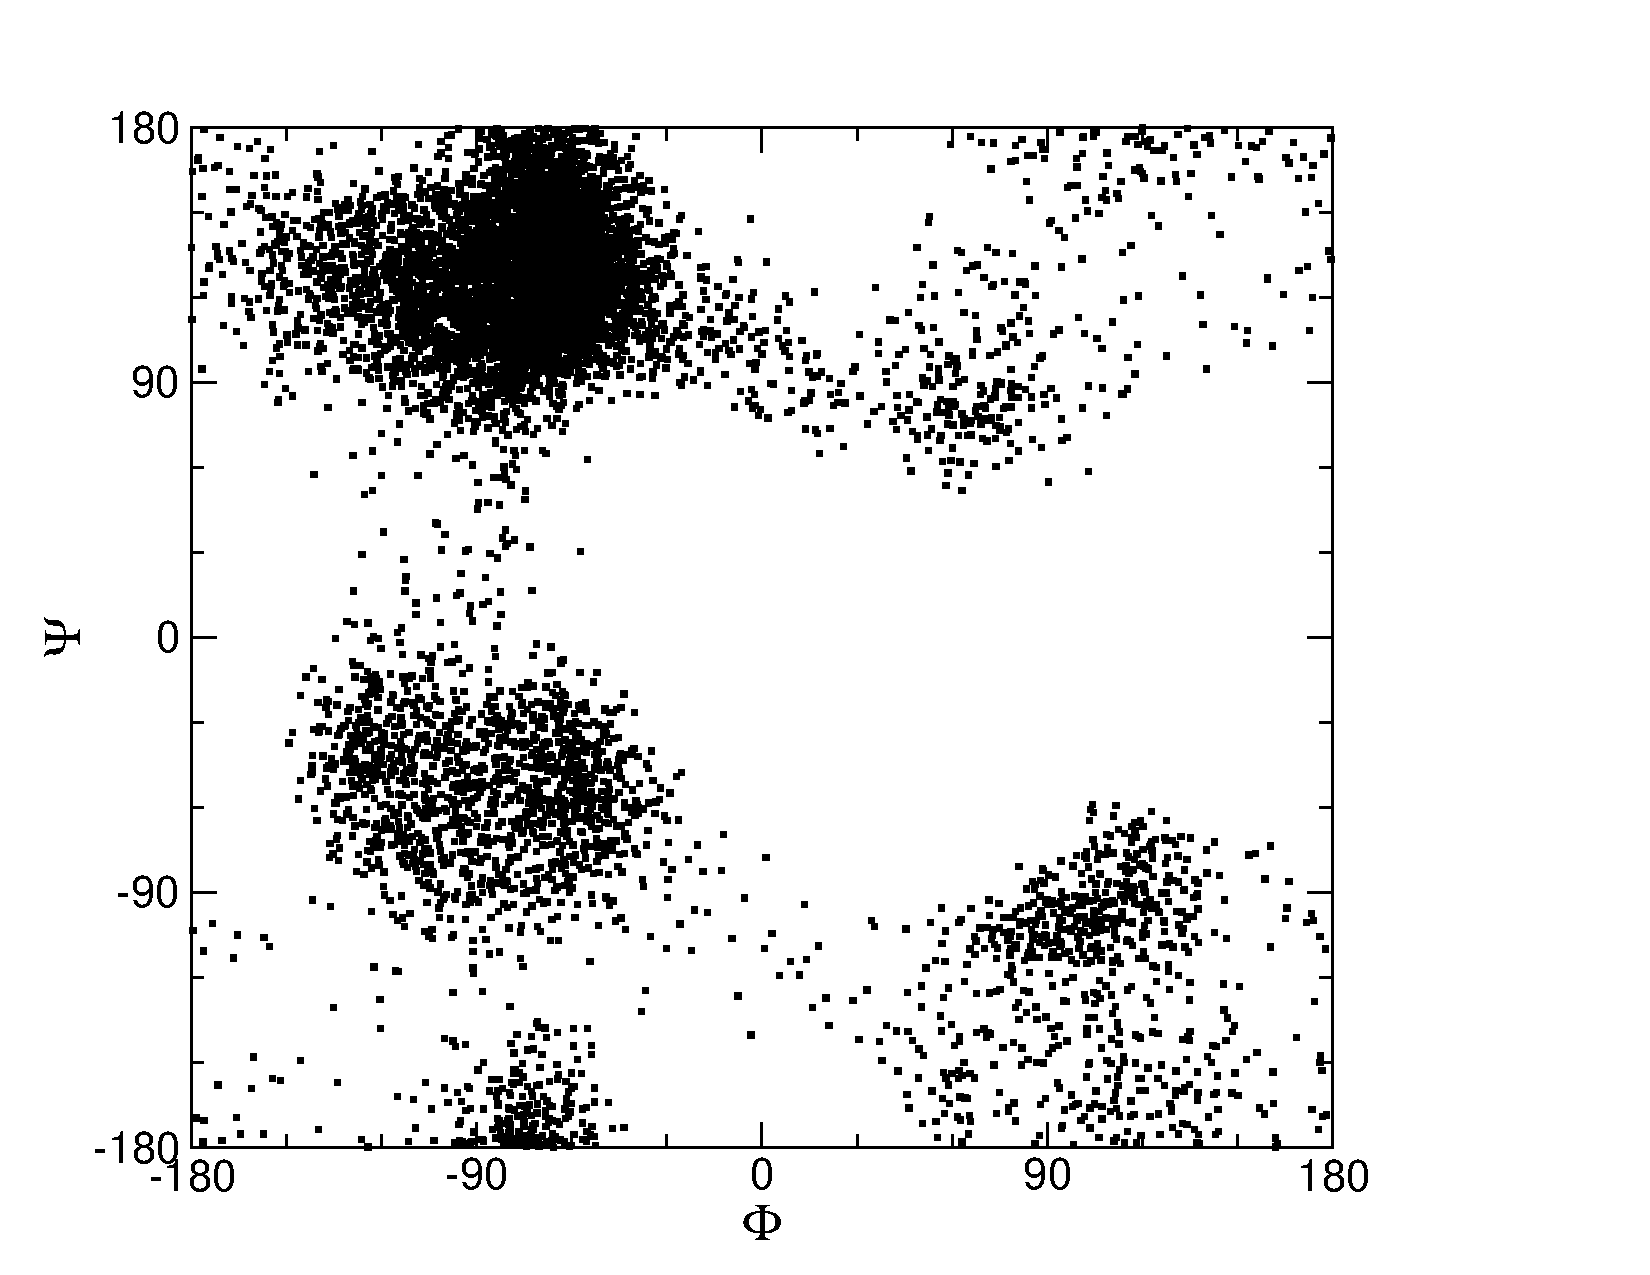
\includegraphics[width=8cm]{plots/rama}}}
\caption{Ramachandran plot of a small protein.}
\label{fig:rama}
\end{figure}

It is also possible to generate an animation of the Ramachandran plot
in time. This can be useful for analyzing certain dihedral transitions 
in your protein. You can use the program {\tt \normindex{g_xrama}} for this.

When studying $\alpha$-helices 
it is useful to have a {\em helical wheel} projection
of your peptide, to see whether a peptide is amphipathic. This can be done
using the {\tt \normindex{g_wheel}} program. Two examples are 
plotted in \figref{wheel}.

\begin{figure}
\centerline{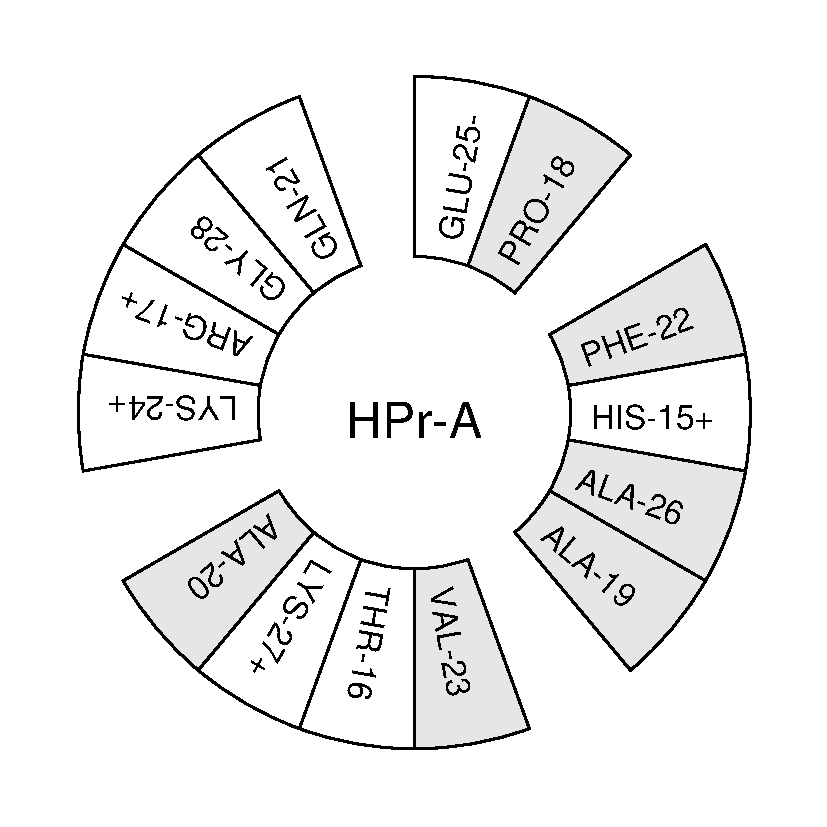
\includegraphics[width=\htw]{plots/hpr-wheel}}
\caption{Helical wheel projection of the N-terminal helix of HPr.}
\label{fig:wheel}
\end{figure}

%%%%%%%%%%%%%%%%%%%%%%%%%%%%%%%%%%%%%%% Membrane Related Items

\section{Interface-related items}
{\tt g_order, g_density, g_potential, g_traj}\\
When simulating molecules with long carbon tails, it can be
interesting to calculate their average orientation. There are several
flavors of order parameters, most of which are related. The program
{\tt \normindex{g_order}} can calculate order parameters using the equation:

\begin{equation}
S_{z} = \frac{3}{2}\langle {\cos^2{\theta_z}} \rangle - \frac{1}{2}
\label{eqn:Sgr}
\end{equation}
where $\theta_z$ is the angle between the $z$-axis of the simulation
box and the molecular axis under consideration. The latter is defined as the
vector from C$_{n-1}$ to C$_{n+1}$. The parameters $S_x$
and $S_y$ are defined in the same way. The brackets imply averaging over time
and molecules. Order parameters can vary between 1 (full order along
the interface normal) and $-1/2$ (full order perpendicular to the
normal), with a value of zero in the case of isotropic orientation.

The program can do two things for you. It can calculate the order
parameter for each CH$_2$ segment separately, for any of three axes,
or it can divide the box in slices and calculate the average value of
the order parameter per segment in one slice. The first method gives
an idea of the ordering of a molecule from head to tail, the second
method gives an idea of the ordering as function of the box length.

The electrostatic potential ($\psi$) across the interface can be
computed from a trajectory by evaluating the double integral of the
charge density ($\rho(z)$):
\beq
\psi(z) - \psi(-\infty) = - \int_{-\infty}^z dz' \int_{-\infty}^{z'} \rho(z'')dz''/ \epsilon_0 
\label{eqn:elpotgr}
\eeq
where the position $z=-\infty$ is far enough in the bulk phase such that
the field is zero.  With this method, it is possible to ``split'' the
total potential into separate contributions from lipid and water
molecules. The program {\tt \normindex{g_potential}} divides the box in slices and
sums all charges of the atoms in each slice. It then integrates this
charge density to give the electric field, which is in turn integrated to
give the potential. Charge density, electric field, and potential are written
to {\tt xvgr} input files.

The program {\tt \normindex{g_traj}} is a very simple analysis program. All it
does is print the coordinates, velocities, or forces of selected atoms.
It can also calculate the center of mass of one or more
molecules and print the coordinates of the center of mass to three
files. By itself, this is probably not a very useful analysis, but
having the coordinates of selected molecules or atoms can be very
handy for further analysis, not only in interfacial systems.

%
% Non-existent program
% The program {\tt \normindex{g_pvd}} calculates a lot of properties, among which
% the density of a group in particles per unit of volume, but not a
% density that takes the mass of the atoms into account. The program
%

The program {\tt \normindex{g_density}} also calculates the density of groups, 
but takes the masses into account and gives a plot of the density against a box
axis. This is useful for looking at the distribution of groups or
atoms across the interface.

%%%%%%%%%%%%%%%%%%%%%%%%%%%%%%%%%%%%%%% Chemical shifts

\section{Chemical shifts}
{\tt total, do_shift}\\
You can compute the NMR chemical shifts of protons with the program
{\tt \normindex{do_shift}}. This is just an {\gromacs} interface to
the public domain program {\tt total}~\cite{Williamson93a}. For
further information, read the article. Although there is limited
support for this in {\gromacs}, users are encouraged to use the
software provided by David Case's group at Scripps because it seems
to be more up-to-date.

%%%%%%%%%%%%%%%%%%%%%%%%%%%%%%%%%%%%%%%
%} % Brace matches ifthenelse test for gmxlite

% LocalWords:  Xmgr ndx mk angndx rdf dihedrals grompp hydrogens MainChain Prot
% LocalWords:  oxygens SideChain tryptophan vsitetop aminoacids dat ngmx dr SPC
% LocalWords:  OO ACF fg xmgr corrmd ACFs kM iM FFT th NMR nd corrleg rotacf dt
% LocalWords:  velacc Kubo msd Tildesley corrtime msdwater sgangle cis dih xpm
% LocalWords:  mindist mdmat rms rmsdist rmsd jj diag eigenvectors covar anaeig
% LocalWords:  macromolecule trr tpr gro pdb nofit hbond rclcl HB multi Luzar
% LocalWords:  dssp rama xrama rg Ramachandran phipsi amphipathic HPr xvgr pvd
% LocalWords:  Scripps RDF

\ifthenelse{\equal{\gmxlite}{1}}{}{
%
%       A P P E N D I C E S
%
\appendix
\chapter{Technical Details.}
\label{ch:install}
\section{Installation.}
The {\gromacs} code is distributed in SOURCE form by our WWW server at\\
{\wwwpage}\\
On this server you will find all the information you need to 
\normindex{install}
the software, as well as the \normindex{license form} that you have to submit
before you are allowed to download the code. When you have filled in this
license form, a username and password will be sent to you by e-mail
with which you can download the files. The e-mail address you specify
on your license sheet will also be used to send you information on
updates, bug-fixes etc.

For \normindex{commercial use} of the software, please contact us directly:
{\tt gromacs@chem.rug.nl}

\section{Porting {\gromacs}.}
The {\gromacs} system is designed with portability as one major design
goal. However there are a number of things we assume to be present on
the system {\gromacs} is being ported on. We assume the following
features:

\begin{enumerate}
\item 	the UNIX operating system (BSD 4.x or SYSTEM V rev.3 or higher) 
	or UNIX-like libraries
\item 	an ANSI C compiler 
\item	a Fortran-77 compiler or Fortran-90 compiler
	for faster (on some computers) innerloop routines
\item 	If you want to use the graphics, the X-window system version 
	11 Release 4 or higher and the X-lib graphics libraries
\end{enumerate}

These are the requirements of a single processor system. If you want
to compile {\gromacs} on a multi processor environment there is another
requirement:

\begin{enumerate}
\item Message-passing architecture
\item Ring structure.
\end{enumerate}

One can understand that a message passing architecture also can be
mapped onto a shared memory machine. This implementation is left to
the reader as an exercise in parallel programming. Also the ring
structure can be mapped onto eg. a hypercube.

\subsection{Multi-processor Porting}

In the case you want to run the {\gromacs} software on a
multi-processor machine, you have two options.
\begin{enumerate}
\item	Install \normindex{MPI} or \normindex{PVM}. The {\gromacs} WWW
	page has some pointers to relevant documents.
\item	Write communication routines yourself. 
\end{enumerate}

It may be clear that you will hardly ever need to write the routines
yourself, but if you can't avoid it, here are some clues.
The interface between these routines and the
rest of the {\gromacs} system is described in the file {\tt
\$GMXHOME/src/include/network.h} We will give a short description of the
different routines below.

{\bf extern void gmx\_tx(int pid,void *buf,int bufsize);}\\ 

This routine, when called with the destination processor number, a
pointer to a (byte oriented) transfer buffer, and the size of the
buffer will send the buffer to the indicated processor (in our case
always the neigbouring processor). The routine does {\bf not} wait
until the transfer is finished.

\smallskip

{\bf extern void gmx\_tx\_wait(int pid);}\\
This routine waits until the previous, or the ongoing transmission is finished.

\smallskip


{\bf extern void gmx\_txs(int pid,void *buf,int bufsize);}\\
This routine implements a synchonous send by calling the async routine and then
the wait. It might come in handy to code this differently.

\smallskip

{\bf extern void gmx\_rx(int pid,void *buf,int bufsize);}\\
{\bf extern void gmx\_rx\_wait(int pid);}\\
{\bf extern void gmx\_rxs(int pid,void *buf,int bufsize);}\\
The very same routines for receiving a buffer and waiting untill the reception is finished.

\smallskip

{\bf extern void gmx\_init(int pid,int nprocs);}\\
This routine initializes the different devices needed to do the communication. In general it sets up the communication hardware (if it is accessible) or does an initalize call to the lower level communication subsystem.

\smallskip

{\bf extern void gmx\_stat(FILE *fp,char *msg);}\\
With this routine we can diagnose the ongoing communication. In the current implementation it prints the various contents of the hardware communication  registers of the (\intel) multiprocessor boards to a file.


\section{Environment Variables}
{\gromacs} programs may be influenced by the use of \normindex{environment} 
variables. First of all, the variables set in the \normindex{GMXRC} file
are essential for running and compiling {\gromacs}. Other variables are:
\begin{enumerate}
\item	\normindex{DUMP\_NL}, dump \normindex{neighborlist}. 
	If set to a positive number the {\em entire}
	neighborlist is printed in the log file (may be many megabytes).
	Mainly for debugging purposes, but may allso be handy for
	\normindex{porting} to other platforms.
\item	\normindex{IAMCOOL}, when set prints \normindex{cool quotes}, otherwise
	your {\gromacs} life will be dull and boring.
\item	\normindex{WHERE}, when set print debugging info on line numbers.
\item	\normindex{LOG\_BUFS}. The size of the buffer for file I/O. When set
	to 0, all file I/O will be unbuffered and therefore very slow.
	This can be handy for debugging purposes, because it ensures
	that all files are always totally up-to-date.
\item   \normindex{GMXNPRI}, for SGI systems only. When set, gives the
	default non-degrading priority (npri) for {\tt
	\normindex{mdrun}}, {\tt \normindex{nmrun}}, {\tt
	\normindex{g\_covar}} and {\tt \normindex{g\_nmeig}},
	e.g.\@ setting \verb'setenv GMXNPRI 250' causes all
	runs to be performed at near-lowest priority by default.
\end{enumerate}

Some other environment variables are specific to one program, such as
\normindex{TOTAL} for the {\tt \normindex{do\_shift}} program, and
\normindex{DSPP} for the {\tt \normindex{do\_dssp}} program.

\section{File types.}
\label{sec:fileformats}
Table~\ref{Tab:form} lists the filetypes used by {\gromacs} along with
a short description.
\begin{table}
\begin{tabularx}{\linewidth}{|r@{\tt.}lccX|}
\dline
\mc{2}{|c}{Default} &      & Default &  \\[-0.1ex]
\mc{1}{|c}{Name} & \mc{1}{c}{Ext.} & Type &  Option & Description \\[-0.1ex]
\hline
\tt   atomtp & \tt atp & Asc & \tt    & Atomtype file used by pdb2gmx \\[-0.1ex]
\tt    eiwit & \tt brk & Asc & \tt -f & Brookhaven data bank file \\[-0.1ex]
\tt   nnnice & \tt dat & Asc & \tt    & Generic data file \\[-0.1ex]
\tt     user & \tt dlg & Asc & \tt    & Dialog Box data for ngmx \\[-0.1ex]
\tt      sam & \tt edi & Asc & \tt    & ED sampling input \\[-0.1ex]
\tt      sam & \tt edo & Asc & \tt    & ED sampling output \\[-0.1ex]
\tt     ener & \tt edr &     & \tt    & Generic energy: \tt edr ene \\[-0.1ex]
\tt     ener & \tt edr & xdr & \tt    & Energy file in portable xdr format \\[-0.1ex]
\tt     ener & \tt ene & Bin & \tt    & Energy file \\[-0.1ex]
\tt    eiwit & \tt ent & Asc & \tt -f & Entry in the protein date bank \\[-0.1ex]
\tt     plot & \tt eps & Asc & \tt    & Encapsulated PostScript (tm) file \\[-0.1ex]
\tt    gtraj & \tt g87 & Asc & \tt    & Gromos-87 ASCII trajectory format \\[-0.1ex]
\tt     conf & \tt g96 & Asc & \tt -c & Coordinate file in Gromos-96 format \\[-0.1ex]
\tt     conf & \tt gro &     & \tt -c & Generic structure: \tt gro g96 pdb tpr tpb tpa \\[-0.1ex]
\tt      out & \tt gro &     & \tt -o & Generic structure: \tt gro g96 pdb \\[-0.1ex]
\tt     conf & \tt gro & Asc & \tt -c & Coordinate file in Gromos-87 format \\[-0.1ex]
\tt    polar & \tt hdb & Asc & \tt    & Hydrogen data base \\[-0.1ex]
\tt   topinc & \tt itp & Asc & \tt    & Include file for topology \\[-0.1ex]
\tt      run & \tt log & Asc & \tt -l & Log file \\[-0.1ex]
\tt       ps & \tt m2p & Asc & \tt    & Input file for mat2ps \\[-0.1ex]
\tt       ss & \tt map & Asc & \tt    & File that maps matrix data to colors \\[-0.1ex]
\tt       ss & \tt mat & Asc & \tt    & Matrix Data file \\[-0.1ex]
\tt   grompp & \tt mdp & Asc & \tt -f & grompp input file with MD parameters \\[-0.1ex]
\tt  hessian & \tt mtx & Bin & \tt -m & Hessian matrix \\[-0.1ex]
\tt    index & \tt ndx & Asc & \tt -n & Index file \\[-0.1ex]
\tt    hello & \tt out & Asc & \tt -o & Generic output file \\[-0.1ex]
\tt    eiwit & \tt pdb & Asc & \tt -f & Protein data bank file \\[-0.1ex]
\tt     pull & \tt pdo & Asc & \tt    & Pull data output \\[-0.1ex]
\tt     pull & \tt ppa & Asc & \tt    & Pull parameters \\[-0.1ex]
\tt  residue & \tt rtp & Asc & \tt    & Residue Type file used by pdb2gmx \\[-0.1ex]
\tt      doc & \tt tex & Asc & \tt -o & LaTeX file \\[-0.1ex]
\tt    topol & \tt top & Asc & \tt -p & Topology file \\[-0.1ex]
\tt    topol & \tt tpa & Asc & \tt -s & Ascii run input file \\[-0.1ex]
\tt    topol & \tt tpb & Bin & \tt -s & Binary run input file \\[-0.1ex]
\tt    topol & \tt tpr &     & \tt -s & Generic run input: \tt tpr tpb tpa \\[-0.1ex]
\tt    topol & \tt tpr &     & \tt -s & Structure+mass(db): \tt tpr tpb tpa gro g96 pdb \\[-0.1ex]
\tt    topol & \tt tpr & xdr & \tt -s & Portable xdr run input file \\[-0.1ex]
\tt     traj & \tt trj & Bin & \tt    & Trajectory file (cpu specific) \\[-0.1ex]
\tt     traj & \tt trr &     & \tt    & Full precision trajectory: \tt trr trj \\[-0.1ex]
\tt     traj & \tt trr & xdr & \tt    & Trajectory in portable xdr format \\[-0.1ex]
\tt     root & \tt xpm & Asc & \tt    & X PixMap compatible matrix file \\[-0.1ex]
\tt     traj & \tt xtc &     & \tt -f & Generic trajectory: \tt xtc trr trj gro g96 pdb \\[-0.1ex]
\tt     traj & \tt xtc & xdr & \tt    & Compressed trajectory (portable xdr format) \\[-0.1ex]
\tt    graph & \tt xvg & Asc & \tt -o & xvgr/xmgr file \\[-0.1ex]
\dline
\end{tabularx}
\caption{The {\gromacs} file types.}
\label{tab:form}
\end{table}


\section{Data types}
Here some of the data types will be described that are necessary for writing
your own analysis programs.

\subsection{Block structure}
The block structure is a datatype that define {\em blocks} of items,
for example molecules can be described as blocks of atom numbers.
In Figure~\ref{fig:block} we have depicted the data structure graphically.
\begin{figure}
\centerline{\psfig{figure=plots/block.eps,width=10cm}}
\caption{Block data structure. Block 4 points to items 7 through 12.}
\label{fig:block}
\end{figure}

Here is, for completeness sake,
the type declaration for the block structure.
\begin{verbatim}
/*
 * Block data structure.
 * This structure is used for charge groups, exclusions
 * molecules and shake-blocks.
 */
typedef struct {
  int multinr[MAXPROC]; /* The indices for the multiprocessor 
                         * version. For n=0, the blocks run from 0
                         * upto multinr[index[0]]. The blocks for 
                         * processor n (n>0) run from 
                         * index[multinr[n-1]] to index[multinr[n]].
                         */
  int nr;               /* The number of blocks                     */
  atom_id *index;       /* Array of indices in a (dim: nr+1)        */
  int nra;              /* The number of atoms                      */
  atom_id *a;           /* Array of atom numbers in each group      */
                        /* (dim: nra)                               */
                        /* Block i (0<=i<nr) runs from              */
                        /* index[i] to index[i+1]-1. There will     */
                        /* allways be an extra entry in index       */
                        /* to terminate the table                   */
} t_block;
\end{verbatim}




%
% This file is part of the GROMACS molecular simulation package.
%
% Copyright (c) 2013,2014,2015, by the GROMACS development team, led by
% Mark Abraham, David van der Spoel, Berk Hess, and Erik Lindahl,
% and including many others, as listed in the AUTHORS file in the
% top-level source directory and at http://www.gromacs.org.
%
% GROMACS is free software; you can redistribute it and/or
% modify it under the terms of the GNU Lesser General Public License
% as published by the Free Software Foundation; either version 2.1
% of the License, or (at your option) any later version.
%
% GROMACS is distributed in the hope that it will be useful,
% but WITHOUT ANY WARRANTY; without even the implied warranty of
% MERCHANTABILITY or FITNESS FOR A PARTICULAR PURPOSE.  See the GNU
% Lesser General Public License for more details.
%
% You should have received a copy of the GNU Lesser General Public
% License along with GROMACS; if not, see
% http://www.gnu.org/licenses, or write to the Free Software Foundation,
% Inc., 51 Franklin Street, Fifth Floor, Boston, MA  02110-1301  USA.
%
% If you want to redistribute modifications to GROMACS, please
% consider that scientific software is very special. Version
% control is crucial - bugs must be traceable. We will be happy to
% consider code for inclusion in the official distribution, but
% derived work must not be called official GROMACS. Details are found
% in the README & COPYING files - if they are missing, get the
% official version at http://www.gromacs.org.
%
% To help us fund GROMACS development, we humbly ask that you cite
% the research papers on the package. Check out http://www.gromacs.org.

\chapter{Some implementation details}
In this chapter we will present some implementation details. This is
far from complete, but we deemed it necessary to clarify some things
that would otherwise be hard to understand.

\section{Single Sum Virial in {\gromacs}}
\label{sec:virial}
The \normindex{virial} $\Xi$ can be written in full tensor form as:
\beq
\Xi~=~-\half~\sum_{i < j}^N~\rvij\otimes\Fvij
\eeq
where $\otimes$ denotes the {\em direct product} of two vectors.\footnote
{$({\bf u}\otimes{\bf v})^{\ab}~=~{\bf u}_{\al}{\bf v}_{\be}$} When this is 
computed in the inner loop of an MD program 9 multiplications and 9
additions are needed.\footnote{The calculation of 
Lennard-Jones and Coulomb forces is about 50 floating point operations.}

Here it is shown how it is possible to extract the virial calculation
from the inner loop~\cite{Bekker93b}.

\subsection{Virial}
In a system with periodic boundary conditions\index{periodic boundary 
conditions}, the
periodicity must be taken into account for the virial:
\beq
\Xi~=~-\half~\sum_{i < j}^{N}~\rnij\otimes\Fvij
\eeq
where $\rnij$ denotes the distance vector of the
{\em nearest image} of atom $i$ from atom $j$. In this definition we add
a {\em shift vector} $\delta_i$ to the position vector $\rvi$ 
of atom $i$. The difference vector $\rnij$ is thus equal to:
\beq
\rnij~=~\rvi+\delta_i-\rvj
\eeq
or in shorthand:
\beq
\rnij~=~\rni-\rvj
\eeq
In a triclinic system, there are 27 possible images of $i$; when a truncated 
octahedron is used, there are 15 possible images.

\subsection{Virial from non-bonded forces}
Here the derivation for the single sum virial in the {\em non-bonded force} 
routine is given. $i \neq j$ in all formulae below.
\newcommand{\di}{\delta_{i}}
\newcommand{\qrt}{\frac{1}{4}}
\bea
\Xi	
&~=~&-\half~\sum_{i < j}^{N}~\rnij\otimes\Fvij				\\
&~=~&-\qrt\sum_{i=1}^N~\sum_{j=1}^N ~(\rvi+\di-\rvj)\otimes\Fvij	\\
&~=~&-\qrt\sum_{i=1}^N~\sum_{j=1}^N ~(\rvi+\di)\otimes\Fvij-\rvj\otimes\Fvij	\\
&~=~&-\qrt\left(\sum_{i=1}^N~\sum_{j=1}^N ~(\rvi+\di)\otimes\Fvij~-~\sum_{i=1}^N~\sum_{j=1}^N ~\rvj\otimes\Fvij\right)	\\
&~=~&-\qrt\left(\sum_{i=1}^N~(\rvi+\di)\otimes\sum_{j=1}^N~\Fvij~-~\sum_{j=1}^N ~\rvj\otimes\sum_{i=1}^N~\Fvij\right)	\\
&~=~&-\qrt\left(\sum_{i=1}^N~(\rvi+\di)\otimes\Fvi~+~\sum_{j=1}^N ~\rvj\otimes\Fvj\right)	\\
&~=~&-\qrt\left(2~\sum_{i=1}^N~\rvi\otimes\Fvi+\sum_{i=1}^N~\di\otimes\Fvi\right)
\eea
In these formulae we introduced:
\bea
\Fvi&~=~&\sum_{j=1}^N~\Fvij					\\
\Fvj&~=~&\sum_{i=1}^N~\Fvji
\eea
which is the total force on $i$ with respect to $j$. Because we use Newton's Third Law:
\beq
\Fvij~=~-\Fvji
\eeq
we must, in the implementation, double the term containing the shift $\delta_i$.

\subsection{The intra-molecular shift (mol-shift)}
For the bonded forces and SHAKE it is possible to make a {\em mol-shift}
list, in which the periodicity is stored. We simple have an array {\tt mshift}
in which for each atom an index in the {\tt shiftvec} array is stored.

The algorithm to generate such a list can be derived from graph theory,
considering each particle in a molecule as a bead in a graph, the bonds 
as edges.
\begin{enumerate}
\item[1]	Represent the bonds and atoms as bidirectional graph
\item[2]	Make all atoms white
\item[3]	Make one of the white atoms black (atom $i$) and put it in the
		central box
\item[4]	Make all of the neighbors of $i$ that are currently 
		white, gray 
\item[5]	Pick one of the gray atoms (atom $j$), give it the
		correct periodicity with respect to any of 
		its black neighbors
		and make it black
\item[6]	Make all of the neighbors of $j$ that are currently 
		white, gray
\item[7]	If any gray atom remains, go to [5]
\item[8]	If any white atom remains, go to [3]
\end{enumerate}
Using this algorithm we can 
\begin{itemize}
\item	optimize the bonded force calculation as well as SHAKE 
\item	calculate the virial from the bonded forces
	in the single sum method again
\end{itemize}

Find a representation of the bonds as a bidirectional graph.

\subsection{Virial from Covalent Bonds}
Since the covalent bond force gives a contribution to the virial, we have:
\bea
b	&~=~&	\|\rnij\|					\\
V_b	&~=~&	\half k_b(b-b_0)^2				\\
\Fvi	&~=~&	-\nabla V_b					\\
	&~=~&	k_b(b-b_0)\frac{\rnij}{b}			\\
\Fvj	&~=~&	-\Fvi
\eea
The virial contribution from the bonds then is:
\bea
\Xi_b	&~=~&	-\half(\rni\otimes\Fvi~+~\rvj\otimes\Fvj)	\\
	&~=~&	-\half\rnij\otimes\Fvi
\eea

\subsection{Virial from SHAKE}
An important contribution to the virial comes from shake. Satisfying 
the constraints a force {\bf G} that is exerted on the particles ``shaken.'' If this
force does not come out of the algorithm (as in standard SHAKE) it can be
calculated afterward (when using {\em leap-frog}) by:
\bea
\Delta\rvi&~=~&\rvi(t+\Dt)-
[\rvi(t)+{\bf v}_i(t-\frac{\Dt}{2})\Dt+\frac{\Fvi}{m_i}\Dt^2]	\\
{\bf G}_i&~=~&\frac{m_i\Delta\rvi}{\Dt^2}
\eea
This does not help us in the general case. Only when no periodicity
is needed (like in rigid water) this can be used, otherwise
we must add the virial calculation in the inner loop of SHAKE.

When it {\em is} applicable the virial can be calculated in the single sum way:
\beq
\Xi~=~-\half\sum_i^{N_c}~\rvi\otimes\Fvi
\eeq
where $N_c$ is the number of constrained atoms.

%Another method is the Non-Iterative shake as proposed (and implemented)
%by Yoneya. In this algorithm the Lagrangian multipliers are solved in a 
%matrix equation, and given these multipliers it is easy to get the periodicity
%in the virial afterwards. 

%More...


\section{Optimizations}
Here we describe some of the algorithmic optimizations used 
in {\gromacs}, apart from parallelism. 
One of these, the implementation of the 
1.0/sqrt(x) function is treated separately in \secref{sqrt}.
The most important other optimizations are described below.

\subsection{Inner Loops for Water}
\label{sec:waterloops}
{\gromacs} uses special inner loops to calculate non-bonded
interactions for water molecules with other atoms, and yet
another set of loops for interactions between pairs of
water molecules. There highly optimized loops for two types of water models.
For three site models similar to
SPC~\cite{Berendsen81}, {\ie}:
\begin{enumerate}
\item   There are three atoms in the molecule.
\item   The whole molecule is a single charge group.
\item   The first atom has Lennard-Jones (\secref{lj}) and 
        Coulomb (\secref{coul}) interactions.
\item   Atoms two and three have only Coulomb interactions, 
        and equal charges.
\end{enumerate}
These loops also works for the SPC/E~\cite{Berendsen87} and 
TIP3P~\cite{Jorgensen83} water models.
And for four site water models similar to TIP4P~\cite{Jorgensen83}:
\begin{enumerate}
\item   There are four atoms in the molecule.
\item   The whole molecule is a single charge group.
\item   The first atom has only Lennard-Jones (\secref{lj}) interactions.
\item   Atoms two and three have only Coulomb (\secref{coul}) interactions, 
        and equal charges.
\item   Atom four has only Coulomb interactions.
\end{enumerate}

The benefit of these implementations is that there are more floating-point
operations in a single loop, which implies that some compilers
can schedule the code better. However, it turns out that even
some of the most advanced compilers have problems with scheduling, 
implying that manual tweaking is necessary to get optimum 
\normindex{performance}.
This may include common-sub-expression elimination, or moving
code around. 

\subsection{Fortran Code}
Unfortunately, on a few platforms \normindex{Fortran} compilers are
still better than C-compilers. For some machines ({\eg} SGI
Power Challenge) the difference may be up to a factor of 3, in the
case of vector computers this may be even larger. Therefore, some of
the routines that take up a lot of computer time have been translated
into Fortran and even assembly code for Intel and AMD x86 processors.
In most cases, the Fortran or assembly loops should be selected 
automatically by the {\tt configure} script when appropriate, but you can
also tweak this by setting options to the {\tt configure} script.

\section{Computation of the 1.0/sqrt function}
\label{sec:sqrt}
\subsection{Introduction}
The {\gromacs} project started with the development of a $1/\sqrt{x}$
processor that calculates:
\begin{equation}
Y(x) = \frac{1}{ \sqrt{x} }
\end{equation}
As the project continued, the {\intel} processor was used to implement
{\gromacs}, which now turned into almost a full software project.  The
$1/\sqrt{x}$ processor was implemented using a Newton-Raphson
iteration scheme for one step. For this it needed look-up tables to
provide the initial approximation. The $1/\sqrt{x}$ function makes it
possible to use two almost independent tables for the exponent seed
and the fraction seed with the IEEE floating-point representation.

\subsection{General}
According to~\cite{Bekker87} the $1/\sqrt{x}$ function can be evaluated using
the Newton-Raphson iteration scheme. The inverse function is:
\begin{equation}
X(y) = \frac{1}{y^{2}}
\end{equation}
So instead of calculating:
\begin{equation}
Y(a) = q
\end{equation}
the equation:
\begin{equation}
X(q) - a = 0
\label{eqn:inversef}
\end{equation}
can now be solved using Newton-Raphson. An iteration is performed by
calculating:
\begin{equation}
y_{n+1} = y_{n} - \frac{f(y_{n})}{f'(y_{n})}
\label{eqn:nr}
\end{equation}
The absolute error $\varepsilon$, in this approximation is defined by:
\begin{equation}
\varepsilon \equiv y_{n} - q
\end{equation}
Using Taylor series expansion to estimate the error results in:
\begin{equation}
\varepsilon _{n+1} = - \frac{\varepsilon _{n}^{2}}{2}
                       \frac{ f''(y_{n})}{f'(y_{n})}
\label{eqn:taylor}
\end{equation}
according to~\cite{Bekker87} equation (3.2). This is an estimation of the
absolute error.

\subsection{Applied to floating-point numbers}
Floating-point numbers in IEEE 32 bit single-precision format have a nearly
constant relative error of $\Delta x / x = 2^{-24}$. As seen earlier in the
Taylor series expansion equation (\eqnref{taylor}), the error in every
iteration step is absolute and in general dependent of $y$. If the error is
expressed as a relative error $\varepsilon_{r}$ the following holds:
\begin{equation}
\varepsilon _{{r}_{n+1}} \equiv \frac{\varepsilon_{n+1}}{y}
\end{equation}
and so:
\begin{equation}
\varepsilon _{{r}_{n+1}} =
- ( \frac{\varepsilon _{n}}{y} )^{2} y \frac{ f''}{2f'}
\end{equation}
For the function $f(y) = y^{-2}$ the term $y f''/2f'$ is constant (equal
to $-3/2$) so the relative error $\varepsilon _{r_{n}}$ is independent of $y$.
\begin{equation}
\varepsilon _{{r}_{n+1}} =
\frac{3}{2} (\varepsilon_{r_{n}})^{2}
\label{eqn:epsr}
\end{equation}

The conclusion of this is that the function $1/\sqrt{x}$ can be
calculated with a specified accuracy.

\begin{figure}
\begin{center}
\newcommand{\twltt}{\tt}
\setlength{\unitlength}{0.0080in}
\begin{picture}(489,176)(40,390)
\thicklines
\put(180,505){$\underbrace{\hspace{2.68in}}$}
\put( 60,505){$\underbrace{\hspace{0.88in}}$}
\put( 40,510){\framebox(480,30){}}
\put( 45,505){\vector( 0,-1){ 15}}
\put( 40,540){\dashbox{4}(0,0){}}
\multiput(250,540)(0.00000,-8.57143){4}{\line( 0,-1){  4.286}}
\multiput(220,540)(0.00000,-8.57143){4}{\line( 0,-1){  4.286}}
\multiput(190,540)(0.00000,-8.57143){4}{\line( 0,-1){  4.286}}
\multiput(280,540)(0.00000,-8.57143){4}{\line( 0,-1){  4.286}}
\multiput(310,540)(0.00000,-8.57143){4}{\line( 0,-1){  4.286}}
\multiput(340,540)(0.00000,-8.57143){4}{\line( 0,-1){  4.286}}
\multiput(370,540)(0.00000,-8.57143){4}{\line( 0,-1){  4.286}}
\multiput(400,540)(0.00000,-8.57143){4}{\line( 0,-1){  4.286}}
\multiput(430,540)(0.00000,-8.57143){4}{\line( 0,-1){  4.286}}
\multiput(460,540)(0.00000,-8.57143){4}{\line( 0,-1){  4.286}}
\multiput(490,540)(0.00000,-8.57143){4}{\line( 0,-1){  4.286}}
\multiput(205,540)(0.00000,-8.57143){4}{\line( 0,-1){  4.286}}
\multiput(235,540)(0.00000,-8.57143){4}{\line( 0,-1){  4.286}}
\multiput(265,540)(0.00000,-8.57143){4}{\line( 0,-1){  4.286}}
\multiput(295,540)(0.00000,-8.57143){4}{\line( 0,-1){  4.286}}
\multiput(325,540)(0.00000,-8.57143){4}{\line( 0,-1){  4.286}}
\multiput(355,540)(0.00000,-8.57143){4}{\line( 0,-1){  4.286}}
\multiput(385,540)(0.00000,-8.57143){4}{\line( 0,-1){  4.286}}
\multiput(415,540)(0.00000,-8.57143){4}{\line( 0,-1){  4.286}}
\multiput(445,540)(0.00000,-8.57143){4}{\line( 0,-1){  4.286}}
\multiput(475,540)(0.00000,-8.57143){4}{\line( 0,-1){  4.286}}
\multiput(505,540)(0.00000,-8.57143){4}{\line( 0,-1){  4.286}}
\put( 40,510){\framebox(480,30){}}
\put( 40,540){\dashbox{4}(0,0){}}
\multiput(250,540)(0.00000,-8.57143){4}{\line( 0,-1){  4.286}}
\multiput(220,540)(0.00000,-8.57143){4}{\line( 0,-1){  4.286}}
\multiput(190,540)(0.00000,-8.57143){4}{\line( 0,-1){  4.286}}
\multiput(160,540)(0.00000,-8.57143){4}{\line( 0,-1){  4.286}}
\multiput(130,540)(0.00000,-8.57143){4}{\line( 0,-1){  4.286}}
\multiput(100,540)(0.00000,-8.57143){4}{\line( 0,-1){  4.286}}
\multiput(280,540)(0.00000,-8.57143){4}{\line( 0,-1){  4.286}}
\multiput(310,540)(0.00000,-8.57143){4}{\line( 0,-1){  4.286}}
\multiput(340,540)(0.00000,-8.57143){4}{\line( 0,-1){  4.286}}
\multiput(370,540)(0.00000,-8.57143){4}{\line( 0,-1){  4.286}}
\multiput(400,540)(0.00000,-8.57143){4}{\line( 0,-1){  4.286}}
\multiput(430,540)(0.00000,-8.57143){4}{\line( 0,-1){  4.286}}
\multiput(460,540)(0.00000,-8.57143){4}{\line( 0,-1){  4.286}}
\multiput(490,540)(0.00000,-8.57143){4}{\line( 0,-1){  4.286}}
\multiput( 70,540)(0.00000,-8.57143){4}{\line( 0,-1){  4.286}}
\put( 55,540){\line( 0,-1){ 30}}
\multiput( 85,540)(0.00000,-8.57143){4}{\line( 0,-1){  4.286}}
\multiput(115,540)(0.00000,-8.57143){4}{\line( 0,-1){  4.286}}
\multiput(145,540)(0.00000,-8.57143){4}{\line( 0,-1){  4.286}}
\multiput(205,540)(0.00000,-8.57143){4}{\line( 0,-1){  4.286}}
\multiput(235,540)(0.00000,-8.57143){4}{\line( 0,-1){  4.286}}
\multiput(265,540)(0.00000,-8.57143){4}{\line( 0,-1){  4.286}}
\multiput(295,540)(0.00000,-8.57143){4}{\line( 0,-1){  4.286}}
\multiput(325,540)(0.00000,-8.57143){4}{\line( 0,-1){  4.286}}
\multiput(355,540)(0.00000,-8.57143){4}{\line( 0,-1){  4.286}}
\multiput(385,540)(0.00000,-8.57143){4}{\line( 0,-1){  4.286}}
\multiput(415,540)(0.00000,-8.57143){4}{\line( 0,-1){  4.286}}
\multiput(445,540)(0.00000,-8.57143){4}{\line( 0,-1){  4.286}}
\multiput(475,540)(0.00000,-8.57143){4}{\line( 0,-1){  4.286}}
\multiput(505,540)(0.00000,-8.57143){4}{\line( 0,-1){  4.286}}
\put(175,540){\line( 0,-1){ 30}}
\put(175,540){\line( 0,-1){ 30}}
\multiput(145,540)(0.00000,-8.57143){4}{\line( 0,-1){  4.286}}
\multiput(115,540)(0.00000,-8.57143){4}{\line( 0,-1){  4.286}}
\multiput( 85,540)(0.00000,-8.57143){4}{\line( 0,-1){  4.286}}
\put( 55,540){\line( 0,-1){ 30}}
\multiput( 70,540)(0.00000,-8.57143){4}{\line( 0,-1){  4.286}}
\multiput(100,540)(0.00000,-8.57143){4}{\line( 0,-1){  4.286}}
\multiput(130,540)(0.00000,-8.57143){4}{\line( 0,-1){  4.286}}
\multiput(160,540)(0.00000,-8.57143){4}{\line( 0,-1){  4.286}}
\put(345,470){\makebox(0,0)[lb]{\raisebox{0pt}[0pt][0pt]{\twltt $F$}}}
\put(110,470){\makebox(0,0)[lb]{\raisebox{0pt}[0pt][0pt]{\twltt $E$}}}
\put( 40,470){\makebox(0,0)[lb]{\raisebox{0pt}[0pt][0pt]{\twltt $S$}}}
\put(505,545){\makebox(0,0)[lb]{\raisebox{0pt}[0pt][0pt]{\twltt $0$}}}
\put(160,545){\makebox(0,0)[lb]{\raisebox{0pt}[0pt][0pt]{\twltt $23$}}}
\put( 40,545){\makebox(0,0)[lb]{\raisebox{0pt}[0pt][0pt]{\twltt $31$}}}
\put(140,400){\makebox(0,0)[lb]{\raisebox{0pt}[0pt][0pt]{\twltt $Value=(-1)^{S}(2^{E-127})(1.F)$}}}
\put(505,545){\makebox(0,0)[lb]{\raisebox{0pt}[0pt][0pt]{\twltt $0$}}}
\put(160,545){\makebox(0,0)[lb]{\raisebox{0pt}[0pt][0pt]{\twltt $23$}}}
\put( 40,545){\makebox(0,0)[lb]{\raisebox{0pt}[0pt][0pt]{\twltt $31$}}}
\put(140,400){\makebox(0,0)[lb]{\raisebox{0pt}[0pt][0pt]{\twltt $Value=(-1)^{S}(2^{E-127})(1.F)$}}}
\end{picture}
\end{center}
\caption{IEEE single-precision floating-point format}
\label{fig:ieee}
\end{figure}

\subsection{Specification of the look-up table}
To calculate the function $1/\sqrt{x}$ using the previously mentioned
iteration scheme, it is clear that the first estimation of the solution must
be accurate enough to get precise results. The requirements for the
calculation are
\begin{itemize}
\item Maximum possible accuracy with the used IEEE format
\item Use only one iteration step for maximum speed
\end{itemize}

The first requirement states that the result of $1/\sqrt{x}$ may have a
relative error $\varepsilon_{r}$ equal to the $\varepsilon_{r}$ of a IEEE 32
bit single-precision floating-point number. From this, the $1/\sqrt{x}$
of the initial approximation can be derived, rewriting the definition of
the relative error for succeeding steps (\eqnref{epsr}):
\begin{equation}
\frac{\varepsilon_{n}}{y} =
\sqrt{\varepsilon_ {r_{n+1}} \frac{2f'}{yf''}}
\end{equation}
So for the look-up table the needed accuracy is:
\begin{equation}
\frac{\Delta Y}{Y} = \sqrt{\frac{2}{3} 2^{-24}}
\label{eqn:accy}
\end{equation}
which defines the width of the table that must be $\geq 13$ bit.

At this point the relative error, $\varepsilon_{r_{n}}$, of the look-up table
is known. From this the maximum relative error in the argument can be 
calculated as follows. The absolute error $\Delta x$ is defined as:
\begin{equation}
\Delta x \equiv \frac{\Delta Y}{Y'}
\end{equation}
and thus:
\begin{equation}
\frac{\Delta x}{Y} = \frac{\Delta Y}{Y} (Y')^{-1}
\end{equation}
and thus:
\begin{equation}
\Delta x = constant \frac{Y}{Y'}
\end{equation}
For the $1/\sqrt{x}$ function, $Y / Y' \sim x$ holds, so
$\Delta x / x = constant$. This is a property of the used floating-point
representation as earlier mentioned. The needed accuracy of the argument of the
look-up table follows from:
\begin{equation}
\frac{\Delta x}{x} = -2 \frac{\Delta Y}{Y}
\end{equation}
So, using the floating-point accuracy (\eqnref{accy}):
\begin{equation}
\frac{\Delta x}{x} = -2 \sqrt{\frac{2}{3} 2^{-24}}
\end{equation}
This defines the length of the look-up table which should be $\geq 12$ bit.

\subsection{Separate exponent and fraction computation}
The used IEEE 32 bit single-precision floating-point format specifies
that a number is represented by a exponent and a fraction. The previous 
section specifies for every possible floating-point number the look-up table 
length and width. Only the size of the fraction of a floating-point number 
defines the accuracy. The conclusion from this can be that the size of the 
look-up table is length of look-up table, earlier specified, times the size of 
the exponent ($2^{12}2^{8}, 1Mb$). The $1/\sqrt{x}$  function has the 
property that the exponent is independent of the fraction. This becomes clear 
if the floating-point representation is used. Define:
\begin{equation}
x \equiv (-1)^{S}(2^{E-127})(1.F)
\label{eqn:fpdef}
\end{equation}
See \figref{ieee}, where $0 \leq S \leq 1$, $0 \leq E \leq 255$,
$1 \leq 1.F < 2$ and $S$, $E$, $F$ integer (normalization conditions). 
The sign bit ($S$) can be omitted because $1/\sqrt{x}$ is only defined 
for $x > 0$. The $1/\sqrt{x}$ function applied to $x$ results in:
\begin{equation}
y(x) = \frac{1}{\sqrt{x}}
\end{equation}
or:
\begin{equation}
y(x) = \frac{1}{\sqrt{(2^{E-127})(1.F)}}
\end{equation}
This can be rewritten as:
\begin{equation}
y(x) = (2^{E-127})^{-1/2}(1.F)^{-1/2}
\label{eqn:yx}
\end{equation}
Define:
\begin{equation}
(2^{E'-127}) \equiv (2^{E-127})^{-1/2}
\end{equation}
\begin{equation}
1.F'\equiv (1.F)^{-1/2}
\end{equation}
Then $\frac{1}{\sqrt{2}} < 1.F' \leq 1$ holds, so the condition
$1 \leq 1.F' < 2$, which is essential for normalized real representation, is
not valid anymore. By introducing an extra term, this can be corrected.
Rewrite the $1/\sqrt{x}$ function applied to floating-point numbers (\eqnref{yx}) as:
\begin{equation}
y(x) = (2^{\frac{127-E}{2}-1}) (2(1.F)^{-1/2})
\end{equation}
and:
\begin{equation}
(2^{E'-127}) \equiv (2^{\frac{127-E}{2}-1})
\label{eqn:exp}
\end{equation}
\begin{equation}
1.F'\equiv 2(1.F)^{-1/2}
\label{eqn:frac}
\end{equation}
Then $\sqrt{2} < 1.F \leq 2$ holds. This is not the exact valid range as
defined for normalized floating-point numbers in \eqnref{fpdef}. 
The value $2$  causes the problem. By mapping this value on the nearest
representation $< 2$, this can be solved. The small error that is introduced
by this approximation is within the allowable range. 

The integer representation of the exponent is the next problem. Calculating
$(2^{\frac{127-E}{2}-1})$ introduces a fractional result if $(127-E) = odd$.
This is again easily accounted for by splitting up the calculation into an
odd and an even part. For $(127-E) = even$ $E'$ in equation (\eqnref{exp})
can be exactly calculated in integer arithmetic as a function of $E$.
\begin{equation}
E' = \frac{127-E}{2} + 126
\end{equation}

For $(127-E) = odd$ equation (\eqnref{yx}) can be rewritten as:
\begin{equation}
y(x) = (2^{\frac{127-E-1}{2}})(\frac{1.F}{2})^{-1/2}
\end{equation}
Thus:
\begin{equation}
E' = \frac{126-E}{2} + 127
\end{equation}
which also can be calculated exactly in integer arithmetic.
{\bf Note} that the fraction is automatically corrected for its range earlier
mentioned, so the exponent does not need an extra correction.

The conclusions from this are:
\begin{itemize}
\item The fraction and exponent look-up table are independent. The fraction
look-up table exists of two tables (odd and even exponent) so the odd/even
information of the exponent (lsb bit) has to be used to select the right
table.
\item The exponent table is an 256 x 8 bit table, initialized for $odd$
and $even$.% as specified before
\end{itemize}

\subsection{Implementation}
The look-up tables can be generated by a small C program, which uses
floating-point numbers and operations with IEEE 32 bit single-precision format.
Note that because of the $odd$/$even$ information that is needed, the
fraction table is twice the size earlier specified (13 bit i.s.o. 12 bit).
%\figref{expgen} in the appendix shows how to fill the exponent table,
%\figref{fractgen} shows how to fill the fraction table.

The function according to~\eqnref{nr} has to be implemented. 
Applied to the $1/\sqrt{x}$ function, equation~\eqnref{inversef} leads to:
\begin{equation}
f = a - \frac{1}{y^{2}}
\end{equation}
and so:
\begin{equation}
f' = \frac{2}{y^{3}}
\end{equation}
so:
\begin{equation}
y_{n+1} = y_{n} - \frac{ a - \frac{1}{y^{2}_{n}} }{ \frac{2}{y^{3}_{n}} }
\end{equation}
or:
\begin{equation}
y_{n+1} = \frac{y_{n}}{2} (3 - a y^{2}_{n})
\end{equation}
Where $y_{0}$ can be found in the look-up tables, and $y_{1}$ gives the result
to the maximum accuracy. 
%In \figref{as_implementation}) the assembler implementation is given. 
It is clear that only one iteration extra (in double 
precision) is needed for a double-precision result.

% LocalWords:  Virial virial triclinic intra mol mshift shiftvec sqrt SPC lj yf
% LocalWords:  coul Fortran SGI AMD Raphson IEEE taylor epsr accy ieee yx fpdef
% LocalWords:  lsb nr inversef src formulae GROMACS

%
% This file is part of the GROMACS molecular simulation package.
%
% Copyright (c) 2013,2014, by the GROMACS development team, led by
% Mark Abraham, David van der Spoel, Berk Hess, and Erik Lindahl,
% and including many others, as listed in the AUTHORS file in the
% top-level source directory and at http://www.gromacs.org.
%
% GROMACS is free software; you can redistribute it and/or
% modify it under the terms of the GNU Lesser General Public License
% as published by the Free Software Foundation; either version 2.1
% of the License, or (at your option) any later version.
%
% GROMACS is distributed in the hope that it will be useful,
% but WITHOUT ANY WARRANTY; without even the implied warranty of
% MERCHANTABILITY or FITNESS FOR A PARTICULAR PURPOSE.  See the GNU
% Lesser General Public License for more details.
%
% You should have received a copy of the GNU Lesser General Public
% License along with GROMACS; if not, see
% http://www.gnu.org/licenses, or write to the Free Software Foundation,
% Inc., 51 Franklin Street, Fifth Floor, Boston, MA  02110-1301  USA.
%
% If you want to redistribute modifications to GROMACS, please
% consider that scientific software is very special. Version
% control is crucial - bugs must be traceable. We will be happy to
% consider code for inclusion in the official distribution, but
% derived work must not be called official GROMACS. Details are found
% in the README & COPYING files - if they are missing, get the
% official version at http://www.gromacs.org.
%
% To help us fund GROMACS development, we humbly ask that you cite
% the research papers on the package. Check out http://www.gromacs.org.

%%%%%%%%%%%%%%%%%%%%%%%%%%%%%%%%%%%%%%%%%%%%%%%%%%%%%%%%%%%%%%%%%%%%%%%%%
%
%       AVERAGES AND FLUCTUATIONS
%
%%%%%%%%%%%%%%%%%%%%%%%%%%%%%%%%%%%%%%%%%%%%%%%%%%%%%%%%%%%%%%%%%%%%%%%%%
\chapter{Averages and fluctuations}
\section{Formulae for averaging}
{\bf Note:} this section was taken from ref~\cite{Gunsteren94a}.

When analyzing a MD trajectory averages $\left<x\right>$ and fluctuations
\beq
 \left<(\Delta x)^2\right>^{\half} ~=~ \left<[x-\left<x\right>]^2\right>^{\half}
\label{eqn:var0}
\eeq
of a quantity $x$ are to be computed.
The variance $\sigma_x$ of a series of N$_x$ values, 
\{x$_i$\}, can be computed from
\beq
\sigma_x~=~ \sum_{i=1}^{N_x} x_i^2 ~-~  \frac{1}{N_x}\left(\sum_{i=1}^{N_x}x_i\right)^2
\label{eqn:var1}
\eeq
Unfortunately this formula is numerically not very accurate, 
especially when $\sigma_x^{\half}$ is small compared to the values of $x_i$. 
The following (equivalent) expression is numerically more accurate
\beq
\sigma_x ~=~ \sum_{i=1}^{N_x} [x_i  - \left<x\right>]^2
\eeq
with
\beq
  \left<x\right> ~=~ \frac{1}{N_x} \sum_{i=1}^{N_x} x_i
\label{eqn:var2}
\eeq
Using ~\eqnsref{var1}{var2} one has to go 
through the series of $x_i$ values twice, once to determine 
$\left<x\right>$ and again to 
compute $\sigma_x$, 
whereas \eqnref{var0} requires only one sequential scan of
the series \{x$_i$\}. However, one may cast \eqnref{var1} in
another form, containing partial sums, which allows for a sequential 
update algorithm. Define the partial sum
\beq
          X_{n,m} ~=~ \sum_{i=n}^{m} x_i                      
\eeq
and the partial variance
\beq
    \sigma_{n,m} ~=~ \sum_{i=n}^{m}  \left[x_i - \frac{X_{n,m}}{m-n+1}\right]^2  
\label{eqn:sigma}
\eeq
It can be shown that
\beq
          X_{n,m+k} ~=~  X_{n,m} + X_{m+1,m+k}         
\label{eqn:Xpartial}
\eeq
and
\bea
\sigma_{n,m+k} &=& \sigma_{n,m} + \sigma_{m+1,m+k} + \left[~\frac {X_{n,m}}{m-n+1} - \frac{X_{n,m+k}}{m+k-n+1}~\right]^2~* \nonumber\\
   && ~\frac{(m-n+1)(m+k-n+1)}{k}
\label{eqn:varpartial}
\eea
For $n=1$ one finds
\beq
\sigma_{1,m+k} ~=~ \sigma_{1,m} + \sigma_{m+1,m+k}~+~
  \left[~\frac{X_{1,m}}{m} - \frac{X_{1,m+k}}{m+k}~\right]^2~ \frac{m(m+k)}{k}
\label{eqn:sig1}
\eeq
and for $n=1$ and $k=1$ ~(\eqnref{varpartial}) becomes
\bea
\sigma_{1,m+1}  &=& \sigma_{1,m} + 
                        \left[\frac{X_{1,m}}{m} - \frac{X_{1,m+1}}{m+1}\right]^2 m(m+1)\\
                &=& \sigma_{1,m} + 
                        \frac {[~X_{1,m} - m x_{m+1}~]^2}{m(m+1)}
\label{eqn:simplevar0}
\eea
where we have used the relation
\beq
     X_{1,m+1} ~=~  X_{1,m} + x_{m+1}                       
\label{eqn:simplevar1}
\eeq
Using formulae~(\eqnref{simplevar0}) and ~(\eqnref{simplevar1}) the average 
\beq
\left<x\right> ~=~ \frac{X_{1,N_x}}{N_x}
\eeq
and the fluctuation 
\beq
\left<(\Delta x)^2\right>^{\half} = \left[\frac {\sigma_{1,N_x}}{N_x}\right]^{\half}
\eeq
can be obtained by one sweep through the data. 

\section{Implementation}
In {\gromacs} the instantaneous
energies $E(m)$ are stored in the \swapindex{energy}{file}, along with the 
values of $\sigma_{1,m}$ and $X_{1,m}$. Although the steps are counted from 0,
for the energy and fluctuations steps are counted from 1. This means that the
equations presented here are the ones that are implemented.
We give somewhat lengthy derivations in this section
to simplify checking of code and equations later on.

\subsection{Part of a Simulation}
It is not uncommon to perform a simulation where the first part,
{\eg} 100 ps, is taken as \normindex{equilibration}. However, the
averages and fluctuations as printed in the \swapindex{log}{file}
are computed over the whole simulation. The equilibration time,
which is now part of the simulation, may in such a case invalidate the
averages and fluctuations, because these numbers are now dominated
by the initial drift towards equilibrium.

Using~\eqnsref{Xpartial}{varpartial} the average and 
standard deviation over part of the trajectory can be computed as:
\bea
X_{m+1,m+k}     &=& X_{1,m+k} - X_{1,m}                 \\
\sigma_{m+1,m+k} &=& \sigma_{1,m+k}-\sigma_{1,m} - \left[~\frac{X_{1,m}}{m} - \frac{X_{1,m+k}}{m+k}~\right]^{2}~ \frac{m(m+k)}{k}
\eea

or, more generally (with $p \geq 1$ and $q \geq p$):
\bea
X_{p,q}         &=&     X_{1,q} - X_{1,p-1}     \\
\sigma_{p,q}    &=&     \sigma_{1,q}-\sigma_{1,p-1} - \left[~\frac{X_{1,p-1}}{p-1} - \frac{X_{1,q}}{q}~\right]^{2}~ \frac{(p-1)q}{q-p+1}
\eea
{\bf Note} that implementation of this is not entirely trivial, since energies
are not stored every time step of the simulation. We therefore have to construct
$X_{1,p-1}$ and $\sigma_{1,p-1}$ from the information at time $p$ using
\eqnsref{simplevar0}{simplevar1}:
\bea
X_{1,p-1}       &=&     X_{1,p} - x_p   \\
\sigma_{1,p-1}  &=&     \sigma_{1,p} -  \frac {[~X_{1,p-1} - (p-1) x_{p}~]^2}{(p-1)p}
\eea

\subsection{Combining two simulations}
Another frequently occurring problem is, that the fluctuations of two simulations
must be combined. Consider the following example: we have two simulations
(A) of $n$ and (B) of $m$ steps, in which the second simulation is a 
continuation of the first. However, the second simulation starts numbering from 1
instead of from $n+1$. For the partial sum
this is no problem, we have to add $X_{1,n}^A$ from run A:
\beq
X_{1,n+m}^{AB} ~=~ X_{1,n}^A + X_{1,m}^B
\label{eqn:pscomb}
\eeq
When we want to compute the partial variance from the two components we have to 
make a correction $\Delta\sigma$:
\beq
\sigma_{1,n+m}^{AB} ~=~ \sigma_{1,n}^A + \sigma_{1,m}^B +\Delta\sigma
\eeq
if we define $x_i^{AB}$ as the combined and renumbered set of data points we can 
write:
\beq
\sigma_{1,n+m}^{AB} ~=~ \sum_{i=1}^{n+m}  \left[x_i^{AB} - \frac{X_{1,n+m}^{AB}}{n+m}\right]^2  
\eeq
and thus
\beq
\sum_{i=1}^{n+m}  \left[x_i^{AB} - \frac{X_{1,n+m}^{AB}}{n+m}\right]^2  ~=~
\sum_{i=1}^{n}  \left[x_i^{A} - \frac{X_{1,n}^{A}}{n}\right]^2  +
\sum_{i=1}^{m}  \left[x_i^{B} - \frac{X_{1,m}^{B}}{m}\right]^2  +\Delta\sigma
\eeq
or
\bea
\sum_{i=1}^{n+m}  \left[(x_i^{AB})^2 - 2 x_i^{AB}\frac{X^{AB}_{1,n+m}}{n+m} + \left(\frac{X^{AB}_{1,n+m}}{n+m}\right)^2  \right] &-& \nonumber \\
\sum_{i=1}^{n}  \left[(x_i^{A})^2 - 2 x_i^{A}\frac{X^A_{1,n}}{n} + \left(\frac{X^A_{1,n}}{n}\right)^2  \right] &-& \nonumber \\
\sum_{i=1}^{m}  \left[(x_i^{B})^2 - 2 x_i^{B}\frac{X^B_{1,m}}{m} + \left(\frac{X^B_{1,m}}{m}\right)^2  \right] &=& \Delta\sigma
\eea
all the $x_i^2$ terms drop out, and the terms independent of the summation
counter $i$ can be simplified:
\bea
\frac{\left(X^{AB}_{1,n+m}\right)^2}{n+m} \,-\, 
\frac{\left(X^A_{1,n}\right)^2}{n} \,-\, 
\frac{\left(X^B_{1,m}\right)^2}{m} &-& \nonumber \\
2\,\frac{X^{AB}_{1,n+m}}{n+m}\sum_{i=1}^{n+m}x_i^{AB} \,+\,
2\,\frac{X^{A}_{1,n}}{n}\sum_{i=1}^{n}x_i^{A} \,+\,
2\,\frac{X^{B}_{1,m}}{m}\sum_{i=1}^{m}x_i^{B} &=& \Delta\sigma
\eea
we recognize the three partial sums on the second line and use \eqnref{pscomb}
to obtain:
\beq
\Delta\sigma ~=~ \frac{\left(mX^A_{1,n} - nX^B_{1,m}\right)^2}{nm(n+m)}
\eeq
if we check this by inserting $m=1$ we get back \eqnref{simplevar0}

\subsection{Summing energy terms}
The {\tt \normindex{g_energy}} program can also sum energy terms into one, {\eg} 
potential + kinetic = total. For the partial averages this is again easy
if we have $S$ energy components $s$:
\beq
X_{m,n}^S ~=~ \sum_{i=m}^n \sum_{s=1}^S x_i^s ~=~ \sum_{s=1}^S \sum_{i=m}^n x_i^s ~=~ \sum_{s=1}^S X_{m,n}^s
\label{eqn:sumterms}
\eeq
For the fluctuations it is less trivial again, considering for example 
that the fluctuation in potential and kinetic energy should cancel. 
Nevertheless we can try the same approach as before by writing:
\beq
\sigma_{m,n}^S ~=~ \sum_{s=1}^S \sigma_{m,n}^s + \Delta\sigma
\eeq
if we fill in \eqnref{sigma}:
\beq
\sum_{i=m}^n \left[\left(\sum_{s=1}^S x_i^s\right) - \frac{X_{m,n}^S}{m-n+1}\right]^2 ~=~
\sum_{s=1}^S \sum_{i=m}^n \left[\left(x_i^s\right) - \frac{X_{m,n}^s}{m-n+1}\right]^2 + \Delta\sigma
\label{eqn:sigmaterms}
\eeq
which we can expand to:
\bea
&~&\sum_{i=m}^n \left[\sum_{s=1}^S (x_i^s)^2 + \left(\frac{X_{m,n}^S}{m-n+1}\right)^2 -2\left(\frac{X_{m,n}^S}{m-n+1}\sum_{s=1}^S x_i^s + \sum_{s=1}^S \sum_{s'=s+1}^S x_i^s x_i^{s'} \right)\right]    \nonumber \\
&-&\sum_{s=1}^S \sum_{i=m}^n \left[(x_i^s)^2 - 2\,\frac{X_{m,n}^s}{m-n+1}\,x_i^s + \left(\frac{X_{m,n}^s}{m-n+1}\right)^2\right] ~=~\Delta\sigma 
\eea
the terms with $(x_i^s)^2$ cancel, so that we can simplify to:
\bea
&~&\frac{\left(X_{m,n}^S\right)^2}{m-n+1} -2 \frac{X_{m,n}^S}{m-n+1}\sum_{i=m}^n\sum_{s=1}^S x_i^s -2\sum_{i=m}^n\sum_{s=1}^S \sum_{s'=s+1}^S x_i^s x_i^{s'}\, -        \nonumber \\
&~&\sum_{s=1}^S \sum_{i=m}^n \left[- 2\,\frac{X_{m,n}^s}{m-n+1}\,x_i^s + \left(\frac{X_{m,n}^s}{m-n+1}\right)^2\right] ~=~\Delta\sigma 
\eea
or
\beq
-\frac{\left(X_{m,n}^S\right)^2}{m-n+1}  -2\sum_{i=m}^n\sum_{s=1}^S \sum_{s'=s+1}^S x_i^s x_i^{s'}\, +  \sum_{s=1}^S \frac{\left(X_{m,n}^s\right)^2}{m-n+1}  ~=~\Delta\sigma 
\eeq
If we now expand the first term using \eqnref{sumterms} we obtain:
\beq
-\frac{\left(\sum_{s=1}^SX_{m,n}^s\right)^2}{m-n+1}  -2\sum_{i=m}^n\sum_{s=1}^S \sum_{s'=s+1}^S x_i^s x_i^{s'}\, +      \sum_{s=1}^S \frac{\left(X_{m,n}^s\right)^2}{m-n+1}  ~=~\Delta\sigma 
\eeq
which we can reformulate to:
\beq
-2\left[\sum_{s=1}^S \sum_{s'=s+1}^S X_{m,n}^s X_{m,n}^{s'}\,+\sum_{i=m}^n\sum_{s=1}^S \sum_{s'=s+1}^S x_i^s x_i^{s'}\right] ~=~\Delta\sigma 
\eeq
or
\beq
-2\left[\sum_{s=1}^S X_{m,n}^s \sum_{s'=s+1}^S X_{m,n}^{s'}\,+\,\sum_{s=1}^S \sum_{i=m}^nx_i^s \sum_{s'=s+1}^S x_i^{s'}\right] ~=~\Delta\sigma 
\eeq
which gives
\beq
-2\sum_{s=1}^S \left[X_{m,n}^s \sum_{s'=s+1}^S \sum_{i=m}^n x_i^{s'}\,+\,\sum_{i=m}^n x_i^s \sum_{s'=s+1}^S x_i^{s'}\right] ~=~\Delta\sigma 
\eeq
Since we need all data points $i$ to evaluate this, in general this is not possible.
We can then make an estimate of $\sigma_{m,n}^S$ using only the data points that 
are available using the left hand side of \eqnref{sigmaterms}. While the average can
be computed using all time steps in the simulation, the accuracy of the
fluctuations is thus limited by the frequency with which energies are saved.
Since this can be easily done with a program such as \normindex{xmgr} this is not 
built-in in {\gromacs}.

% LocalWords:  Formulae varpartial formulae simplevar Xpartial pscomb mX nX SX
% LocalWords:  sumterms nx sigmaterms xmgr ps nm

} % Brace matches ifthenelse test for gmxlite
%
% The pdfdummy counter is a workaround to get correct
% bookmarks for the index & bibliography in pdf files

\newcounter{pdfdummy}

%
%       B I B L I O G R A P H Y
%
\cleardoublepage
\refstepcounter{pdfdummy}

\addcontentsline{toc}{chapter}{Bibliography}

\bibliographystyle{proteins}
\bibliography{monster,unpubl}

%
%       I N D E X
%
\cleardoublepage
\refstepcounter{pdfdummy}

\ifthenelse{\equal{\gmxlite}{1}}{}{
\addcontentsline{toc}{chapter}{Index}

\renewcommand{\see}[2]{\mbox{} \mbox{\textit{see} #1}}
\printindex
} % Brace matches ifthenelse test for gmxlite

\end{document}

% LocalWords:  Groningen der Spoel Lindahl Nijenborgh Carsten Kutzner Aldert
% LocalWords:  Buuren Apol Meulenhoff Tieleman Sijbers Feenstra Rudi Drunen Sij
% LocalWords:  Berendsen pretention bers ser anual Uppsala Mainz unpubl
% LocalWords:  Bioinformatics GROMACS Rossen Apostolov ar Bjelkmar
% LocalWords:  Fritsch Gerrit Groenhof Junghans Kasson Larsson Peiter
% LocalWords:  Teemu Murtola Szil ard Pronk Jochen Lambeth Lemkul
% LocalWords:  Marklund Maarten
